\documentclass[twoside]{book}

% Packages required by doxygen
\usepackage{calc}
\usepackage{doxygen}
\usepackage{graphicx}
\usepackage[utf8]{inputenc}
\usepackage{makeidx}
\usepackage{multicol}
\usepackage{multirow}
\usepackage{textcomp}
\usepackage[table]{xcolor}

% Font selection
\usepackage[T1]{fontenc}
\usepackage{mathptmx}
\usepackage[scaled=.90]{helvet}
\usepackage{courier}
\usepackage{amssymb}
\usepackage{sectsty}
\renewcommand{\familydefault}{\sfdefault}
\allsectionsfont{%
  \fontseries{bc}\selectfont%
  \color{darkgray}%
}
\renewcommand{\DoxyLabelFont}{%
  \fontseries{bc}\selectfont%
  \color{darkgray}%
}

% Page & text layout
\usepackage{geometry}
\geometry{%
  a4paper,%
  top=2.5cm,%
  bottom=2.5cm,%
  left=2.5cm,%
  right=2.5cm%
}
\tolerance=750
\hfuzz=15pt
\hbadness=750
\setlength{\emergencystretch}{15pt}
\setlength{\parindent}{0cm}
\setlength{\parskip}{0.2cm}
\makeatletter
\renewcommand{\paragraph}{%
  \@startsection{paragraph}{4}{0ex}{-1.0ex}{1.0ex}{%
    \normalfont\normalsize\bfseries\SS@parafont%
  }%
}
\renewcommand{\subparagraph}{%
  \@startsection{subparagraph}{5}{0ex}{-1.0ex}{1.0ex}{%
    \normalfont\normalsize\bfseries\SS@subparafont%
  }%
}
\makeatother

% Headers & footers
\usepackage{fancyhdr}
\pagestyle{fancyplain}
\fancyhead[LE]{\fancyplain{}{\bfseries\thepage}}
\fancyhead[CE]{\fancyplain{}{}}
\fancyhead[RE]{\fancyplain{}{\bfseries\leftmark}}
\fancyhead[LO]{\fancyplain{}{\bfseries\rightmark}}
\fancyhead[CO]{\fancyplain{}{}}
\fancyhead[RO]{\fancyplain{}{\bfseries\thepage}}
\fancyfoot[LE]{\fancyplain{}{}}
\fancyfoot[CE]{\fancyplain{}{}}
\fancyfoot[RE]{\fancyplain{}{\bfseries\scriptsize Generated on Thu Sep 12 2013 11:27:07 for Mage Rage by Doxygen }}
\fancyfoot[LO]{\fancyplain{}{\bfseries\scriptsize Generated on Thu Sep 12 2013 11:27:07 for Mage Rage by Doxygen }}
\fancyfoot[CO]{\fancyplain{}{}}
\fancyfoot[RO]{\fancyplain{}{}}
\renewcommand{\footrulewidth}{0.4pt}
\renewcommand{\chaptermark}[1]{%
  \markboth{#1}{}%
}
\renewcommand{\sectionmark}[1]{%
  \markright{\thesection\ #1}%
}

% Indices & bibliography
\usepackage{natbib}
\usepackage[titles]{tocloft}
\setcounter{tocdepth}{3}
\setcounter{secnumdepth}{5}
\makeindex

% Hyperlinks (required, but should be loaded last)
\usepackage{ifpdf}
\ifpdf
  \usepackage[pdftex,pagebackref=true]{hyperref}
\else
  \usepackage[ps2pdf,pagebackref=true]{hyperref}
\fi
\hypersetup{%
  colorlinks=true,%
  linkcolor=blue,%
  citecolor=blue,%
  unicode%
}

% Custom commands
\newcommand{\clearemptydoublepage}{%
  \newpage{\pagestyle{empty}\cleardoublepage}%
}


%===== C O N T E N T S =====

\begin{document}

% Titlepage & ToC
\hypersetup{pageanchor=false}
\pagenumbering{roman}
\begin{titlepage}
\vspace*{7cm}
\begin{center}%
{\Large Mage Rage }\\
\vspace*{1cm}
{\large Generated by Doxygen 1.8.4}\\
\vspace*{0.5cm}
{\small Thu Sep 12 2013 11:27:07}\\
\end{center}
\end{titlepage}
\clearemptydoublepage
\tableofcontents
\clearemptydoublepage
\pagenumbering{arabic}
\hypersetup{pageanchor=true}

%--- Begin generated contents ---
\chapter{Hierarchical Index}
\section{Class Hierarchy}
This inheritance list is sorted roughly, but not completely, alphabetically\-:\begin{DoxyCompactList}
\item \contentsline{section}{c\-\_\-associative\-\_\-array}{\pageref{classc__associative__array}}{}
\item \contentsline{section}{c\-\_\-game}{\pageref{classc__game}}{}
\item \contentsline{section}{c\-\_\-graphic\-\_\-object}{\pageref{classc__graphic__object}}{}
\begin{DoxyCompactList}
\item \contentsline{section}{c\-\_\-animation}{\pageref{classc__animation}}{}
\item \contentsline{section}{c\-\_\-character}{\pageref{classc__character}}{}
\begin{DoxyCompactList}
\item \contentsline{section}{c\-\_\-monster\-\_\-character}{\pageref{classc__monster__character}}{}
\item \contentsline{section}{c\-\_\-player\-\_\-character}{\pageref{classc__player__character}}{}
\end{DoxyCompactList}
\item \contentsline{section}{c\-\_\-map}{\pageref{classc__map}}{}
\item \contentsline{section}{c\-\_\-map\-\_\-object}{\pageref{classc__map__object}}{}
\end{DoxyCompactList}
\item \contentsline{section}{c\-\_\-menu}{\pageref{classc__menu}}{}
\item \contentsline{section}{t\-\_\-game\-\_\-settings}{\pageref{structt__game__settings}}{}
\item \contentsline{section}{t\-\_\-input\-\_\-output\-\_\-state}{\pageref{structt__input__output__state}}{}
\item \contentsline{section}{t\-\_\-map\-\_\-square}{\pageref{structt__map__square}}{}
\item \contentsline{section}{t\-\_\-missile}{\pageref{structt__missile}}{}
\end{DoxyCompactList}

\chapter{Class Index}
\section{Class List}
Here are the classes, structs, unions and interfaces with brief descriptions\-:\begin{DoxyCompactList}
\item\contentsline{section}{\hyperlink{classc__animation}{c\-\_\-animation} }{\pageref{classc__animation}}{}
\item\contentsline{section}{\hyperlink{classc__associative__array}{c\-\_\-associative\-\_\-array} }{\pageref{classc__associative__array}}{}
\item\contentsline{section}{\hyperlink{classc__character}{c\-\_\-character} }{\pageref{classc__character}}{}
\item\contentsline{section}{\hyperlink{classc__game}{c\-\_\-game} }{\pageref{classc__game}}{}
\item\contentsline{section}{\hyperlink{classc__graphic__object}{c\-\_\-graphic\-\_\-object} }{\pageref{classc__graphic__object}}{}
\item\contentsline{section}{\hyperlink{classc__map}{c\-\_\-map} }{\pageref{classc__map}}{}
\item\contentsline{section}{\hyperlink{classc__map__object}{c\-\_\-map\-\_\-object} }{\pageref{classc__map__object}}{}
\item\contentsline{section}{\hyperlink{classc__menu}{c\-\_\-menu} }{\pageref{classc__menu}}{}
\item\contentsline{section}{\hyperlink{classc__monster__character}{c\-\_\-monster\-\_\-character} }{\pageref{classc__monster__character}}{}
\item\contentsline{section}{\hyperlink{classc__player__character}{c\-\_\-player\-\_\-character} }{\pageref{classc__player__character}}{}
\item\contentsline{section}{\hyperlink{structt__game__settings}{t\-\_\-game\-\_\-settings} }{\pageref{structt__game__settings}}{}
\item\contentsline{section}{\hyperlink{structt__input__output__state}{t\-\_\-input\-\_\-output\-\_\-state} }{\pageref{structt__input__output__state}}{}
\item\contentsline{section}{\hyperlink{structt__map__square}{t\-\_\-map\-\_\-square} }{\pageref{structt__map__square}}{}
\item\contentsline{section}{\hyperlink{structt__missile}{t\-\_\-missile} }{\pageref{structt__missile}}{}
\end{DoxyCompactList}

\chapter{Class Documentation}
\hypertarget{classc__animation}{\section{c\-\_\-animation Class Reference}
\label{classc__animation}\index{c\-\_\-animation@{c\-\_\-animation}}
}
Inheritance diagram for c\-\_\-animation\-:\begin{figure}[H]
\begin{center}
\leavevmode
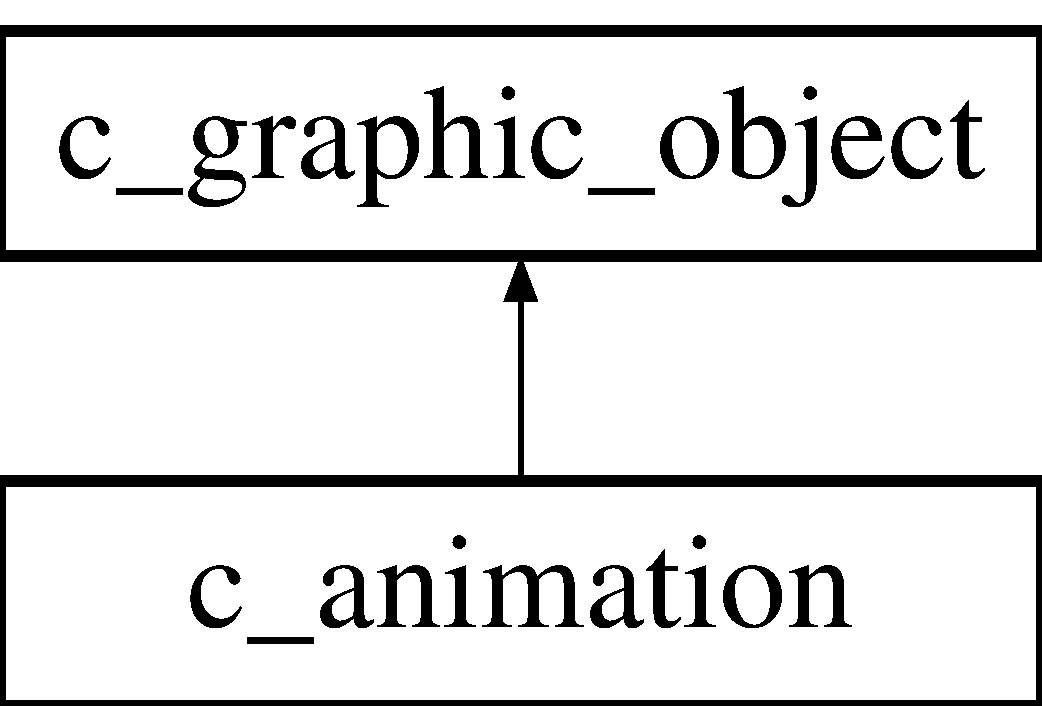
\includegraphics[height=2.000000cm]{classc__animation}
\end{center}
\end{figure}
\subsection*{Public Member Functions}
\begin{DoxyCompactItemize}
\item 
\hyperlink{classc__animation_af98386490424ee6265da7edd9bf6436f}{c\-\_\-animation} (long int $\ast$\hyperlink{classc__graphic__object_a9ff91aa7a60272a8f713ff011a0cc0bb}{global\-\_\-time}, string file\-\_\-prefix, int number\-\_\-of\-\_\-frames, int \hyperlink{classc__animation_a94a4d0e669cf48082e293c8d811e5ca4}{offset\-\_\-x}, int \hyperlink{classc__animation_acb05e62189bcbac633c9290016c25415}{offset\-\_\-y}, int \hyperlink{classc__animation_acbb0e4a3a678ecf74b91e23c22eaa29a}{speed}, bool has\-\_\-sound, string sound\-\_\-path, double \hyperlink{classc__graphic__object_a8274f6e9f1221b91be61ca923e1dc03c}{sound\-\_\-gain})
\item 
\hyperlink{classc__animation_a1b4c0a7b17edb2ac92daa6fbd8afcd93}{$\sim$c\-\_\-animation} ()
\item 
virtual void \hyperlink{classc__animation_a36d69237de6781450680a38717385721}{draw} (int x, int y)
\end{DoxyCompactItemize}
\subsection*{Protected Attributes}
\begin{DoxyCompactItemize}
\item 
int \hyperlink{classc__animation_acbb0e4a3a678ecf74b91e23c22eaa29a}{speed}
\item 
int \hyperlink{classc__animation_a94a4d0e669cf48082e293c8d811e5ca4}{offset\-\_\-x}
\item 
int \hyperlink{classc__animation_acb05e62189bcbac633c9290016c25415}{offset\-\_\-y}
\item 
A\-L\-L\-E\-G\-R\-O\-\_\-\-B\-I\-T\-M\-A\-P $\ast$ \hyperlink{classc__animation_ad881d6653de035e33a8b0ad3e0c178a5}{frames} \mbox{[}M\-A\-X\-\_\-\-A\-N\-I\-M\-A\-T\-I\-O\-N\-\_\-\-F\-R\-A\-M\-E\-S\mbox{]}
\end{DoxyCompactItemize}


\subsection{Constructor \& Destructor Documentation}
\hypertarget{classc__animation_af98386490424ee6265da7edd9bf6436f}{\index{c\-\_\-animation@{c\-\_\-animation}!c\-\_\-animation@{c\-\_\-animation}}
\index{c\-\_\-animation@{c\-\_\-animation}!c_animation@{c\-\_\-animation}}
\subsubsection[{c\-\_\-animation}]{\setlength{\rightskip}{0pt plus 5cm}c\-\_\-animation\-::c\-\_\-animation (
\begin{DoxyParamCaption}
\item[{long int $\ast$}]{global\-\_\-time, }
\item[{string}]{file\-\_\-prefix, }
\item[{int}]{number\-\_\-of\-\_\-frames, }
\item[{int}]{offset\-\_\-x, }
\item[{int}]{offset\-\_\-y, }
\item[{int}]{speed, }
\item[{bool}]{has\-\_\-sound, }
\item[{string}]{sound\-\_\-path, }
\item[{double}]{sound\-\_\-gain}
\end{DoxyParamCaption}
)}}\label{classc__animation_af98386490424ee6265da7edd9bf6436f}
bitmaps-\/ animation frames

Animation object class implementation.

authors\-: Miloslav Číž year\-: 2013 \hypertarget{classc__animation_a1b4c0a7b17edb2ac92daa6fbd8afcd93}{\index{c\-\_\-animation@{c\-\_\-animation}!$\sim$c\-\_\-animation@{$\sim$c\-\_\-animation}}
\index{$\sim$c\-\_\-animation@{$\sim$c\-\_\-animation}!c_animation@{c\-\_\-animation}}
\subsubsection[{$\sim$c\-\_\-animation}]{\setlength{\rightskip}{0pt plus 5cm}c\-\_\-animation\-::$\sim$c\-\_\-animation (
\begin{DoxyParamCaption}
{}
\end{DoxyParamCaption}
)}}\label{classc__animation_a1b4c0a7b17edb2ac92daa6fbd8afcd93}
Class constructor, initialises a new object.


\begin{DoxyParams}{Parameters}
{\em global\-\_\-time} & reference to a global time counter \\
\hline
{\em file\-\_\-prefix} & string prefix of file names, that contain the animation frames -\/ for example if \char`\"{}a\char`\"{} is specified and number of frames is 3, then this method will search for files \char`\"{}a\-\_\-1.\-png\char`\"{}, \char`\"{}a\-\_\-2.\-png\char`\"{} and \char`\"{}a\-\_\-3.\-png\char`\"{} \\
\hline
{\em number\-\_\-of\-\_\-frames} & number of animation frames (there must be corresponding number of png files) \\
\hline
{\em offset\-\_\-x} & x offset for drawing in pixels (can be negative) \\
\hline
{\em offset\-\_\-y} & y offset for drawing in pixels (can be negative) \\
\hline
{\em speed} & speed of the animation, 1 is normal, 2 is twice as slow and so on \\
\hline
{\em has\-\_\-sound} & set this to true if sound should be loaded for this animation, otherwise false \\
\hline
{\em sound\-\_\-path} & if the previous parameter is true, this specifies the path to the sound file \\
\hline
{\em sound\-\_\-gain} & sound gain (volume), 1.\-0 is normal \\
\hline
\end{DoxyParams}


\subsection{Member Function Documentation}
\hypertarget{classc__animation_a36d69237de6781450680a38717385721}{\index{c\-\_\-animation@{c\-\_\-animation}!draw@{draw}}
\index{draw@{draw}!c_animation@{c\-\_\-animation}}
\subsubsection[{draw}]{\setlength{\rightskip}{0pt plus 5cm}void c\-\_\-animation\-::draw (
\begin{DoxyParamCaption}
\item[{int}]{x, }
\item[{int}]{y}
\end{DoxyParamCaption}
)\hspace{0.3cm}{\ttfamily [virtual]}}}\label{classc__animation_a36d69237de6781450680a38717385721}
Class destructor, frees all it's memory. 

Reimplemented from \hyperlink{classc__graphic__object_a94ef8137eed9ce1ae7adf366fefb51cf}{c\-\_\-graphic\-\_\-object}.



\subsection{Member Data Documentation}
\hypertarget{classc__animation_ad881d6653de035e33a8b0ad3e0c178a5}{\index{c\-\_\-animation@{c\-\_\-animation}!frames@{frames}}
\index{frames@{frames}!c_animation@{c\-\_\-animation}}
\subsubsection[{frames}]{\setlength{\rightskip}{0pt plus 5cm}A\-L\-L\-E\-G\-R\-O\-\_\-\-B\-I\-T\-M\-A\-P$\ast$ c\-\_\-animation\-::frames\mbox{[}M\-A\-X\-\_\-\-A\-N\-I\-M\-A\-T\-I\-O\-N\-\_\-\-F\-R\-A\-M\-E\-S\mbox{]}\hspace{0.3cm}{\ttfamily [protected]}}}\label{classc__animation_ad881d6653de035e33a8b0ad3e0c178a5}
y offset for drawing in pixels \hypertarget{classc__animation_a94a4d0e669cf48082e293c8d811e5ca4}{\index{c\-\_\-animation@{c\-\_\-animation}!offset\-\_\-x@{offset\-\_\-x}}
\index{offset\-\_\-x@{offset\-\_\-x}!c_animation@{c\-\_\-animation}}
\subsubsection[{offset\-\_\-x}]{\setlength{\rightskip}{0pt plus 5cm}int c\-\_\-animation\-::offset\-\_\-x\hspace{0.3cm}{\ttfamily [protected]}}}\label{classc__animation_a94a4d0e669cf48082e293c8d811e5ca4}
animation speed, 1 is normal, 2 is twice as slow and so on \hypertarget{classc__animation_acb05e62189bcbac633c9290016c25415}{\index{c\-\_\-animation@{c\-\_\-animation}!offset\-\_\-y@{offset\-\_\-y}}
\index{offset\-\_\-y@{offset\-\_\-y}!c_animation@{c\-\_\-animation}}
\subsubsection[{offset\-\_\-y}]{\setlength{\rightskip}{0pt plus 5cm}int c\-\_\-animation\-::offset\-\_\-y\hspace{0.3cm}{\ttfamily [protected]}}}\label{classc__animation_acb05e62189bcbac633c9290016c25415}
x offset for drawing in pixels \hypertarget{classc__animation_acbb0e4a3a678ecf74b91e23c22eaa29a}{\index{c\-\_\-animation@{c\-\_\-animation}!speed@{speed}}
\index{speed@{speed}!c_animation@{c\-\_\-animation}}
\subsubsection[{speed}]{\setlength{\rightskip}{0pt plus 5cm}int c\-\_\-animation\-::speed\hspace{0.3cm}{\ttfamily [protected]}}}\label{classc__animation_acbb0e4a3a678ecf74b91e23c22eaa29a}
This class represents an animation object. It contains one animation, that can be played on the screen. It does not affect the game itself, only makes it look nicer. 

The documentation for this class was generated from the following files\-:\begin{DoxyCompactItemize}
\item 
magerage/animation.\-h\item 
magerage/animation.\-cpp\end{DoxyCompactItemize}

\hypertarget{classc__associative__array}{\section{c\-\_\-associative\-\_\-array Class Reference}
\label{classc__associative__array}\index{c\-\_\-associative\-\_\-array@{c\-\_\-associative\-\_\-array}}
}


{\ttfamily \#include $<$associative\-\_\-array.\-h$>$}

\subsection*{Public Member Functions}
\begin{DoxyCompactItemize}
\item 
\hyperlink{classc__associative__array_a81ad1750fa1d2c1f48ca77a9c335435f}{c\-\_\-associative\-\_\-array} ()
\item 
\hyperlink{classc__associative__array_a44db0ff9cf78c954d5d8e6645bc3f432}{$\sim$c\-\_\-associative\-\_\-array} ()
\item 
bool \hyperlink{classc__associative__array_a62c94b9c3b92e52885027d77d10d4f0f}{load\-\_\-from\-\_\-file} (string file\-\_\-name)
\item 
bool \hyperlink{classc__associative__array_af01617371af63735362b2a5d2c376ea6}{save\-\_\-to\-\_\-file} (string file\-\_\-name)
\item 
string \hyperlink{classc__associative__array_abc77748614083307465a001ec789ea16}{get\-\_\-text} (string identifier)
\item 
void \hyperlink{classc__associative__array_ab23eae554f876688eead4f6608baa33d}{set\-\_\-text} (string identifier, string value)
\item 
void \hyperlink{classc__associative__array_a32415722135f5d204d77ed739d51f23b}{delete\-\_\-text} (string identifier)
\end{DoxyCompactItemize}
\subsection*{Protected Attributes}
\begin{DoxyCompactItemize}
\item 
\hypertarget{classc__associative__array_a954d95789ca9af971d05509b2c679527}{vector$<$ string $>$ $\ast$ {\bfseries keys}}\label{classc__associative__array_a954d95789ca9af971d05509b2c679527}

\item 
vector$<$ string $>$ $\ast$ \hyperlink{classc__associative__array_a16874608ab16ecb8ef8c9a577c86aa52}{values}
\end{DoxyCompactItemize}


\subsection{Detailed Description}
Associative array class header file.

authors\-: Miloslav Číž, Martin Gabriel year\-: 2013 

\subsection{Constructor \& Destructor Documentation}
\hypertarget{classc__associative__array_a81ad1750fa1d2c1f48ca77a9c335435f}{\index{c\-\_\-associative\-\_\-array@{c\-\_\-associative\-\_\-array}!c\-\_\-associative\-\_\-array@{c\-\_\-associative\-\_\-array}}
\index{c\-\_\-associative\-\_\-array@{c\-\_\-associative\-\_\-array}!c_associative_array@{c\-\_\-associative\-\_\-array}}
\subsubsection[{c\-\_\-associative\-\_\-array}]{\setlength{\rightskip}{0pt plus 5cm}c\-\_\-associative\-\_\-array\-::c\-\_\-associative\-\_\-array (
\begin{DoxyParamCaption}
{}
\end{DoxyParamCaption}
)}}\label{classc__associative__array_a81ad1750fa1d2c1f48ca77a9c335435f}
list of values

Associative array class implementation.

authors\-: Miloslav Číž, Martin Gabriel year\-: 2013 \hypertarget{classc__associative__array_a44db0ff9cf78c954d5d8e6645bc3f432}{\index{c\-\_\-associative\-\_\-array@{c\-\_\-associative\-\_\-array}!$\sim$c\-\_\-associative\-\_\-array@{$\sim$c\-\_\-associative\-\_\-array}}
\index{$\sim$c\-\_\-associative\-\_\-array@{$\sim$c\-\_\-associative\-\_\-array}!c_associative_array@{c\-\_\-associative\-\_\-array}}
\subsubsection[{$\sim$c\-\_\-associative\-\_\-array}]{\setlength{\rightskip}{0pt plus 5cm}c\-\_\-associative\-\_\-array\-::$\sim$c\-\_\-associative\-\_\-array (
\begin{DoxyParamCaption}
{}
\end{DoxyParamCaption}
)}}\label{classc__associative__array_a44db0ff9cf78c954d5d8e6645bc3f432}
Class constructor, initialises a new object. 

\subsection{Member Function Documentation}
\hypertarget{classc__associative__array_a32415722135f5d204d77ed739d51f23b}{\index{c\-\_\-associative\-\_\-array@{c\-\_\-associative\-\_\-array}!delete\-\_\-text@{delete\-\_\-text}}
\index{delete\-\_\-text@{delete\-\_\-text}!c_associative_array@{c\-\_\-associative\-\_\-array}}
\subsubsection[{delete\-\_\-text}]{\setlength{\rightskip}{0pt plus 5cm}void c\-\_\-associative\-\_\-array\-::delete\-\_\-text (
\begin{DoxyParamCaption}
\item[{string}]{identifier}
\end{DoxyParamCaption}
)}}\label{classc__associative__array_a32415722135f5d204d77ed739d51f23b}
Sets the value for given identifier. If the identifier already exists, it's current value will be overwritten, otherwise a new key is created with this value.


\begin{DoxyParams}{Parameters}
{\em identifier} & identifier of the text to be returned \\
\hline
{\em value} & value for the identifier \\
\hline
\end{DoxyParams}
\hypertarget{classc__associative__array_abc77748614083307465a001ec789ea16}{\index{c\-\_\-associative\-\_\-array@{c\-\_\-associative\-\_\-array}!get\-\_\-text@{get\-\_\-text}}
\index{get\-\_\-text@{get\-\_\-text}!c_associative_array@{c\-\_\-associative\-\_\-array}}
\subsubsection[{get\-\_\-text}]{\setlength{\rightskip}{0pt plus 5cm}string c\-\_\-associative\-\_\-array\-::get\-\_\-text (
\begin{DoxyParamCaption}
\item[{string}]{identifier}
\end{DoxyParamCaption}
)}}\label{classc__associative__array_abc77748614083307465a001ec789ea16}
Saves the array to given file.


\begin{DoxyParams}{Parameters}
{\em file\-\_\-name} & path to the file \\
\hline
\end{DoxyParams}
\begin{DoxyReturn}{Returns}
true if the file was saved succesfully, false otherwise 
\end{DoxyReturn}
\hypertarget{classc__associative__array_a62c94b9c3b92e52885027d77d10d4f0f}{\index{c\-\_\-associative\-\_\-array@{c\-\_\-associative\-\_\-array}!load\-\_\-from\-\_\-file@{load\-\_\-from\-\_\-file}}
\index{load\-\_\-from\-\_\-file@{load\-\_\-from\-\_\-file}!c_associative_array@{c\-\_\-associative\-\_\-array}}
\subsubsection[{load\-\_\-from\-\_\-file}]{\setlength{\rightskip}{0pt plus 5cm}bool c\-\_\-associative\-\_\-array\-::load\-\_\-from\-\_\-file (
\begin{DoxyParamCaption}
\item[{string}]{file\-\_\-name}
\end{DoxyParamCaption}
)}}\label{classc__associative__array_a62c94b9c3b92e52885027d77d10d4f0f}
Class destructor, frees all it's memory. \hypertarget{classc__associative__array_af01617371af63735362b2a5d2c376ea6}{\index{c\-\_\-associative\-\_\-array@{c\-\_\-associative\-\_\-array}!save\-\_\-to\-\_\-file@{save\-\_\-to\-\_\-file}}
\index{save\-\_\-to\-\_\-file@{save\-\_\-to\-\_\-file}!c_associative_array@{c\-\_\-associative\-\_\-array}}
\subsubsection[{save\-\_\-to\-\_\-file}]{\setlength{\rightskip}{0pt plus 5cm}bool c\-\_\-associative\-\_\-array\-::save\-\_\-to\-\_\-file (
\begin{DoxyParamCaption}
\item[{string}]{file\-\_\-name}
\end{DoxyParamCaption}
)}}\label{classc__associative__array_af01617371af63735362b2a5d2c376ea6}
Loads the array from given file. The file contains texts separated by newlines, each line in format\-: identifier\-:text


\begin{DoxyParams}{Parameters}
{\em file\-\_\-name} & path to the file \\
\hline
\end{DoxyParams}
\begin{DoxyReturn}{Returns}
true if the file was loaded succesfully, false otherwise 
\end{DoxyReturn}
\hypertarget{classc__associative__array_ab23eae554f876688eead4f6608baa33d}{\index{c\-\_\-associative\-\_\-array@{c\-\_\-associative\-\_\-array}!set\-\_\-text@{set\-\_\-text}}
\index{set\-\_\-text@{set\-\_\-text}!c_associative_array@{c\-\_\-associative\-\_\-array}}
\subsubsection[{set\-\_\-text}]{\setlength{\rightskip}{0pt plus 5cm}void c\-\_\-associative\-\_\-array\-::set\-\_\-text (
\begin{DoxyParamCaption}
\item[{string}]{identifier, }
\item[{string}]{value}
\end{DoxyParamCaption}
)}}\label{classc__associative__array_ab23eae554f876688eead4f6608baa33d}
Returns text with given identifier.


\begin{DoxyParams}{Parameters}
{\em identifier} & identifier of the text to be returned \\
\hline
\end{DoxyParams}
\begin{DoxyReturn}{Returns}
text with given identifier, or (if the text was not found) returns an empty string 
\end{DoxyReturn}


\subsection{Member Data Documentation}
\hypertarget{classc__associative__array_a16874608ab16ecb8ef8c9a577c86aa52}{\index{c\-\_\-associative\-\_\-array@{c\-\_\-associative\-\_\-array}!values@{values}}
\index{values@{values}!c_associative_array@{c\-\_\-associative\-\_\-array}}
\subsubsection[{values}]{\setlength{\rightskip}{0pt plus 5cm}vector$<$string$>$$\ast$ c\-\_\-associative\-\_\-array\-::values\hspace{0.3cm}{\ttfamily [protected]}}}\label{classc__associative__array_a16874608ab16ecb8ef8c9a577c86aa52}
list of keys 

The documentation for this class was generated from the following files\-:\begin{DoxyCompactItemize}
\item 
magerage/associative\-\_\-array.\-h\item 
magerage/associative\-\_\-array.\-cpp\end{DoxyCompactItemize}

\hypertarget{classc__character}{\section{c\-\_\-character Class Reference}
\label{classc__character}\index{c\-\_\-character@{c\-\_\-character}}
}


{\ttfamily \#include $<$character.\-h$>$}

Inheritance diagram for c\-\_\-character\-:\begin{figure}[H]
\begin{center}
\leavevmode
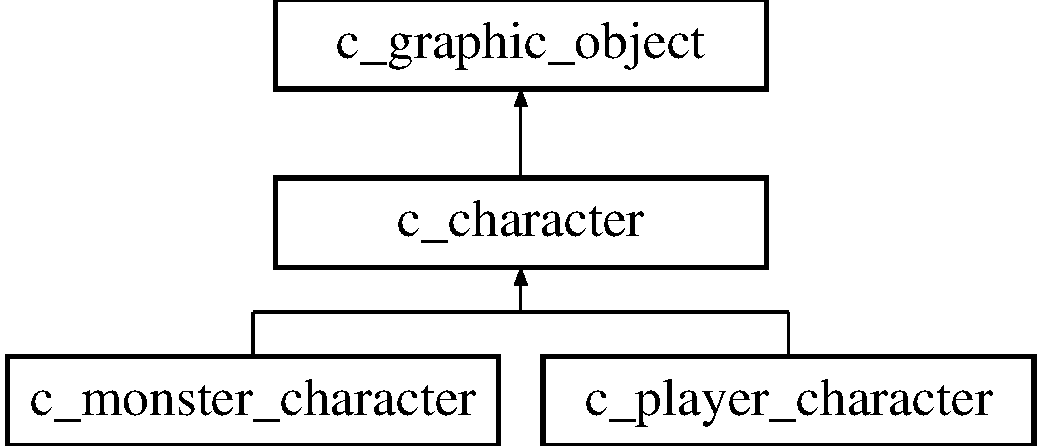
\includegraphics[height=3.000000cm]{classc__character}
\end{center}
\end{figure}
\subsection*{Public Member Functions}
\begin{DoxyCompactItemize}
\item 
void \hyperlink{classc__character_a75c54e9c7283064a4064c6f369d4f45e}{set\-\_\-position} (double x, double y)
\item 
void \hyperlink{classc__character_ace2ad2a0175d52648347a01446d7cc75}{set\-\_\-square\-\_\-position} (int x, int y)
\item 
void \hyperlink{classc__character_a21828380cb11fded91a99dbbc9df9848}{set\-\_\-direction} (t\-\_\-direction \hyperlink{classc__character_a571f1ae6115d7e9fee3159c41fcf27e8}{direction})
\item 
void \hyperlink{classc__character_a4379e618f98e6be9cdf74c4cb723cd4e}{move\-\_\-by} (double x, double y)
\item 
double \hyperlink{classc__character_a74dead1895f81f7e40dc854edcf66ea7}{get\-\_\-position\-\_\-x} ()
\item 
double \hyperlink{classc__character_a1998f04f49c42ca29acb2decdcdcab31}{get\-\_\-position\-\_\-y} ()
\item 
int \hyperlink{classc__character_a00780360179b7b58334bbae046c0a6e6}{get\-\_\-square\-\_\-x} ()
\item 
int \hyperlink{classc__character_ac99f93abd4f6a9dc436ca96a4ff3f856}{get\-\_\-square\-\_\-y} ()
\item 
double \hyperlink{classc__character_a5ffab5363aa4f8661d6c59ccc4e82038}{get\-\_\-fraction\-\_\-x} ()
\item 
double \hyperlink{classc__character_aa2efb20e603bfe0a5b3e63c3ffc86719}{get\-\_\-fraction\-\_\-y} ()
\item 
virtual void \hyperlink{classc__character_a323dd6b7cf6635a0b61e4351178d7518}{loop\-\_\-animation} (t\-\_\-animation\-\_\-type animation)
\item 
t\-\_\-direction \hyperlink{classc__character_af5421aaa7b9ddb2b17e7994419f93c42}{get\-\_\-direction} ()
\end{DoxyCompactItemize}
\subsection*{Static Public Member Functions}
\begin{DoxyCompactItemize}
\item 
static int \hyperlink{classc__character_ae5c54984450cd668f8caff08bab773b9}{position\-\_\-to\-\_\-square} (double position, bool take\-\_\-x)
\item 
static double \hyperlink{classc__character_aef52e1c8a40484d9441867d10aa05b5f}{square\-\_\-to\-\_\-position} (int square\-\_\-position, bool take\-\_\-x)
\end{DoxyCompactItemize}
\subsection*{Protected Attributes}
\begin{DoxyCompactItemize}
\item 
double \hyperlink{classc__character_a09bb0a2dd9eb4a0c7e791706fe51bddc}{position\-\_\-x}
\item 
double \hyperlink{classc__character_a9d37196174588bc6ee1593a2f6c98244}{position\-\_\-y}
\item 
t\-\_\-direction \hyperlink{classc__character_a571f1ae6115d7e9fee3159c41fcf27e8}{direction}
\item 
double \hyperlink{classc__character_a4b50e02f88351baf6dc1542ef97fd413}{footsteps\-\_\-gain}
\item 
double \hyperlink{classc__character_addf8133a5a8cf4ce83405e5a1335fdfd}{skate\-\_\-gain}
\item 
A\-L\-L\-E\-G\-R\-O\-\_\-\-B\-I\-T\-M\-A\-P $\ast$ \hyperlink{classc__character_a7bddca76d4c38008b127fa0d3ea36738}{shadow}
\item 
A\-L\-L\-E\-G\-R\-O\-\_\-\-B\-I\-T\-M\-A\-P $\ast$ \hyperlink{classc__character_a97b679f81ebff4c53933a278a05a11c6}{sprite\-\_\-north}
\item 
A\-L\-L\-E\-G\-R\-O\-\_\-\-B\-I\-T\-M\-A\-P $\ast$ \hyperlink{classc__character_adb3cfdb7715791d21a0ac917b4443b47}{sprite\-\_\-north\-\_\-running\-\_\-1}
\item 
A\-L\-L\-E\-G\-R\-O\-\_\-\-B\-I\-T\-M\-A\-P $\ast$ \hyperlink{classc__character_a009fa720b3902c4517edea6e1195daf5}{sprite\-\_\-north\-\_\-running\-\_\-2}
\item 
A\-L\-L\-E\-G\-R\-O\-\_\-\-B\-I\-T\-M\-A\-P $\ast$ \hyperlink{classc__character_afabf5a5d776707387be05162e7389aa1}{sprite\-\_\-east}
\item 
A\-L\-L\-E\-G\-R\-O\-\_\-\-B\-I\-T\-M\-A\-P $\ast$ \hyperlink{classc__character_ae6f68b43b39ceac377631aa406b43a0b}{sprite\-\_\-east\-\_\-running\-\_\-1}
\item 
A\-L\-L\-E\-G\-R\-O\-\_\-\-B\-I\-T\-M\-A\-P $\ast$ \hyperlink{classc__character_a563e59c84f1cf673bcd1d4b5179727c1}{sprite\-\_\-east\-\_\-running\-\_\-2}
\item 
A\-L\-L\-E\-G\-R\-O\-\_\-\-B\-I\-T\-M\-A\-P $\ast$ \hyperlink{classc__character_a3ca4db7645eb80c31738f5c5dae337a9}{sprite\-\_\-south}
\item 
A\-L\-L\-E\-G\-R\-O\-\_\-\-B\-I\-T\-M\-A\-P $\ast$ \hyperlink{classc__character_af5df98de273f4561fcdc2a51f209ffec}{sprite\-\_\-south\-\_\-running\-\_\-1}
\item 
A\-L\-L\-E\-G\-R\-O\-\_\-\-B\-I\-T\-M\-A\-P $\ast$ \hyperlink{classc__character_a5d3bd19c0e6ebe9e6bf656c33ace7577}{sprite\-\_\-south\-\_\-running\-\_\-2}
\item 
A\-L\-L\-E\-G\-R\-O\-\_\-\-B\-I\-T\-M\-A\-P $\ast$ \hyperlink{classc__character_a2f6f83ee5580e3d89e2170072353001e}{sprite\-\_\-west}
\item 
A\-L\-L\-E\-G\-R\-O\-\_\-\-B\-I\-T\-M\-A\-P $\ast$ \hyperlink{classc__character_a3429225d2f84f44e9f3af4236e6dd731}{sprite\-\_\-west\-\_\-running\-\_\-1}
\item 
A\-L\-L\-E\-G\-R\-O\-\_\-\-B\-I\-T\-M\-A\-P $\ast$ \hyperlink{classc__character_aef269ee1bc3fb08b89a8b254c20e8262}{sprite\-\_\-west\-\_\-running\-\_\-2}
\item 
A\-L\-L\-E\-G\-R\-O\-\_\-\-S\-A\-M\-P\-L\-E $\ast$ \hyperlink{classc__character_af944a0456aa0fdb9720b1dd2b9b4e235}{sound\-\_\-footsteps}
\item 
A\-L\-L\-E\-G\-R\-O\-\_\-\-S\-A\-M\-P\-L\-E $\ast$ \hyperlink{classc__character_a728e0633d8f62df9f08bcce7bea03cee}{sound\-\_\-skate}
\end{DoxyCompactItemize}


\subsection{Detailed Description}
Character class header file.

authors\-: Miloslav Číž year\-: 2013 

\subsection{Member Function Documentation}
\hypertarget{classc__character_af5421aaa7b9ddb2b17e7994419f93c42}{\index{c\-\_\-character@{c\-\_\-character}!get\-\_\-direction@{get\-\_\-direction}}
\index{get\-\_\-direction@{get\-\_\-direction}!c_character@{c\-\_\-character}}
\subsubsection[{get\-\_\-direction}]{\setlength{\rightskip}{0pt plus 5cm}t\-\_\-direction c\-\_\-character\-::get\-\_\-direction (
\begin{DoxyParamCaption}
{}
\end{DoxyParamCaption}
)}}\label{classc__character_af5421aaa7b9ddb2b17e7994419f93c42}
Loops the given animation untill it's stopped by \hyperlink{classc__graphic__object_a32cdba2150d09d903f6e95f2509b9283}{stop\-\_\-animation()}.


\begin{DoxyParams}{Parameters}
{\em animation} & animation to be looped \\
\hline
\end{DoxyParams}
\hypertarget{classc__character_a5ffab5363aa4f8661d6c59ccc4e82038}{\index{c\-\_\-character@{c\-\_\-character}!get\-\_\-fraction\-\_\-x@{get\-\_\-fraction\-\_\-x}}
\index{get\-\_\-fraction\-\_\-x@{get\-\_\-fraction\-\_\-x}!c_character@{c\-\_\-character}}
\subsubsection[{get\-\_\-fraction\-\_\-x}]{\setlength{\rightskip}{0pt plus 5cm}double c\-\_\-character\-::get\-\_\-fraction\-\_\-x (
\begin{DoxyParamCaption}
{}
\end{DoxyParamCaption}
)}}\label{classc__character_a5ffab5363aa4f8661d6c59ccc4e82038}
Returns y coordination of the square at which the character is standing.

\begin{DoxyReturn}{Returns}
y coordination of the character's square 
\end{DoxyReturn}
\hypertarget{classc__character_aa2efb20e603bfe0a5b3e63c3ffc86719}{\index{c\-\_\-character@{c\-\_\-character}!get\-\_\-fraction\-\_\-y@{get\-\_\-fraction\-\_\-y}}
\index{get\-\_\-fraction\-\_\-y@{get\-\_\-fraction\-\_\-y}!c_character@{c\-\_\-character}}
\subsubsection[{get\-\_\-fraction\-\_\-y}]{\setlength{\rightskip}{0pt plus 5cm}double c\-\_\-character\-::get\-\_\-fraction\-\_\-y (
\begin{DoxyParamCaption}
{}
\end{DoxyParamCaption}
)}}\label{classc__character_aa2efb20e603bfe0a5b3e63c3ffc86719}
Returns fraction part of the position, which is position within current square.

\begin{DoxyReturn}{Returns}
x position within current square (value in range $<$0;1$>$) 
\end{DoxyReturn}
\hypertarget{classc__character_a74dead1895f81f7e40dc854edcf66ea7}{\index{c\-\_\-character@{c\-\_\-character}!get\-\_\-position\-\_\-x@{get\-\_\-position\-\_\-x}}
\index{get\-\_\-position\-\_\-x@{get\-\_\-position\-\_\-x}!c_character@{c\-\_\-character}}
\subsubsection[{get\-\_\-position\-\_\-x}]{\setlength{\rightskip}{0pt plus 5cm}double c\-\_\-character\-::get\-\_\-position\-\_\-x (
\begin{DoxyParamCaption}
{}
\end{DoxyParamCaption}
)}}\label{classc__character_a74dead1895f81f7e40dc854edcf66ea7}
Sets the character's position relatively to current position.


\begin{DoxyParams}{Parameters}
{\em x} & value to be added to x position \\
\hline
{\em y} & value to be added to y position \\
\hline
\end{DoxyParams}
\hypertarget{classc__character_a1998f04f49c42ca29acb2decdcdcab31}{\index{c\-\_\-character@{c\-\_\-character}!get\-\_\-position\-\_\-y@{get\-\_\-position\-\_\-y}}
\index{get\-\_\-position\-\_\-y@{get\-\_\-position\-\_\-y}!c_character@{c\-\_\-character}}
\subsubsection[{get\-\_\-position\-\_\-y}]{\setlength{\rightskip}{0pt plus 5cm}double c\-\_\-character\-::get\-\_\-position\-\_\-y (
\begin{DoxyParamCaption}
{}
\end{DoxyParamCaption}
)}}\label{classc__character_a1998f04f49c42ca29acb2decdcdcab31}
Returns x position of the character.

\begin{DoxyReturn}{Returns}
x position 
\end{DoxyReturn}
\hypertarget{classc__character_a00780360179b7b58334bbae046c0a6e6}{\index{c\-\_\-character@{c\-\_\-character}!get\-\_\-square\-\_\-x@{get\-\_\-square\-\_\-x}}
\index{get\-\_\-square\-\_\-x@{get\-\_\-square\-\_\-x}!c_character@{c\-\_\-character}}
\subsubsection[{get\-\_\-square\-\_\-x}]{\setlength{\rightskip}{0pt plus 5cm}int c\-\_\-character\-::get\-\_\-square\-\_\-x (
\begin{DoxyParamCaption}
{}
\end{DoxyParamCaption}
)}}\label{classc__character_a00780360179b7b58334bbae046c0a6e6}
Returns y position of the character.

\begin{DoxyReturn}{Returns}
y position 
\end{DoxyReturn}
\hypertarget{classc__character_ac99f93abd4f6a9dc436ca96a4ff3f856}{\index{c\-\_\-character@{c\-\_\-character}!get\-\_\-square\-\_\-y@{get\-\_\-square\-\_\-y}}
\index{get\-\_\-square\-\_\-y@{get\-\_\-square\-\_\-y}!c_character@{c\-\_\-character}}
\subsubsection[{get\-\_\-square\-\_\-y}]{\setlength{\rightskip}{0pt plus 5cm}int c\-\_\-character\-::get\-\_\-square\-\_\-y (
\begin{DoxyParamCaption}
{}
\end{DoxyParamCaption}
)}}\label{classc__character_ac99f93abd4f6a9dc436ca96a4ff3f856}
Returns x coordination of the square at which the character is standing.

\begin{DoxyReturn}{Returns}
x coordination of the character's square 
\end{DoxyReturn}
\hypertarget{classc__character_a323dd6b7cf6635a0b61e4351178d7518}{\index{c\-\_\-character@{c\-\_\-character}!loop\-\_\-animation@{loop\-\_\-animation}}
\index{loop\-\_\-animation@{loop\-\_\-animation}!c_character@{c\-\_\-character}}
\subsubsection[{loop\-\_\-animation}]{\setlength{\rightskip}{0pt plus 5cm}void c\-\_\-character\-::loop\-\_\-animation (
\begin{DoxyParamCaption}
\item[{t\-\_\-animation\-\_\-type}]{animation}
\end{DoxyParamCaption}
)\hspace{0.3cm}{\ttfamily [virtual]}}}\label{classc__character_a323dd6b7cf6635a0b61e4351178d7518}
Returns fraction part of the position, which is position within current square.

\begin{DoxyReturn}{Returns}
y position within current square (value in range $<$0;1$>$) 
\end{DoxyReturn}


Reimplemented from \hyperlink{classc__graphic__object_ac60b00df5a7edefe4c61e6a59802473f}{c\-\_\-graphic\-\_\-object}.

\hypertarget{classc__character_a4379e618f98e6be9cdf74c4cb723cd4e}{\index{c\-\_\-character@{c\-\_\-character}!move\-\_\-by@{move\-\_\-by}}
\index{move\-\_\-by@{move\-\_\-by}!c_character@{c\-\_\-character}}
\subsubsection[{move\-\_\-by}]{\setlength{\rightskip}{0pt plus 5cm}void c\-\_\-character\-::move\-\_\-by (
\begin{DoxyParamCaption}
\item[{double}]{x, }
\item[{double}]{y}
\end{DoxyParamCaption}
)}}\label{classc__character_a4379e618f98e6be9cdf74c4cb723cd4e}
Sets the character's facing direction.


\begin{DoxyParams}{Parameters}
{\em direction} & new direction\\
\hline
\end{DoxyParams}
Character class implementation file.

authors\-: Miloslav Číž year\-: 2013 \hypertarget{classc__character_ae5c54984450cd668f8caff08bab773b9}{\index{c\-\_\-character@{c\-\_\-character}!position\-\_\-to\-\_\-square@{position\-\_\-to\-\_\-square}}
\index{position\-\_\-to\-\_\-square@{position\-\_\-to\-\_\-square}!c_character@{c\-\_\-character}}
\subsubsection[{position\-\_\-to\-\_\-square}]{\setlength{\rightskip}{0pt plus 5cm}int c\-\_\-character\-::position\-\_\-to\-\_\-square (
\begin{DoxyParamCaption}
\item[{double}]{position, }
\item[{bool}]{take\-\_\-x}
\end{DoxyParamCaption}
)\hspace{0.3cm}{\ttfamily [static]}}}\label{classc__character_ae5c54984450cd668f8caff08bab773b9}
sound -\/ skate \hypertarget{classc__character_a21828380cb11fded91a99dbbc9df9848}{\index{c\-\_\-character@{c\-\_\-character}!set\-\_\-direction@{set\-\_\-direction}}
\index{set\-\_\-direction@{set\-\_\-direction}!c_character@{c\-\_\-character}}
\subsubsection[{set\-\_\-direction}]{\setlength{\rightskip}{0pt plus 5cm}void c\-\_\-character\-::set\-\_\-direction (
\begin{DoxyParamCaption}
\item[{t\-\_\-direction}]{direction}
\end{DoxyParamCaption}
)}}\label{classc__character_a21828380cb11fded91a99dbbc9df9848}
Sets the player's position given in map squares.


\begin{DoxyParams}{Parameters}
{\em x} & \\
\hline
{\em y} & \\
\hline
\end{DoxyParams}
\hypertarget{classc__character_a75c54e9c7283064a4064c6f369d4f45e}{\index{c\-\_\-character@{c\-\_\-character}!set\-\_\-position@{set\-\_\-position}}
\index{set\-\_\-position@{set\-\_\-position}!c_character@{c\-\_\-character}}
\subsubsection[{set\-\_\-position}]{\setlength{\rightskip}{0pt plus 5cm}void c\-\_\-character\-::set\-\_\-position (
\begin{DoxyParamCaption}
\item[{double}]{x, }
\item[{double}]{y}
\end{DoxyParamCaption}
)}}\label{classc__character_a75c54e9c7283064a4064c6f369d4f45e}
Converts position in map squares to double position.


\begin{DoxyParams}{Parameters}
{\em square\-\_\-position} & position in map squares to be converted \\
\hline
{\em take\-\_\-x} & if true, the position is considered as x position, otherwise y position \\
\hline
\end{DoxyParams}
\begin{DoxyReturn}{Returns}
double position 
\end{DoxyReturn}
\hypertarget{classc__character_ace2ad2a0175d52648347a01446d7cc75}{\index{c\-\_\-character@{c\-\_\-character}!set\-\_\-square\-\_\-position@{set\-\_\-square\-\_\-position}}
\index{set\-\_\-square\-\_\-position@{set\-\_\-square\-\_\-position}!c_character@{c\-\_\-character}}
\subsubsection[{set\-\_\-square\-\_\-position}]{\setlength{\rightskip}{0pt plus 5cm}void c\-\_\-character\-::set\-\_\-square\-\_\-position (
\begin{DoxyParamCaption}
\item[{int}]{x, }
\item[{int}]{y}
\end{DoxyParamCaption}
)}}\label{classc__character_ace2ad2a0175d52648347a01446d7cc75}
Sets the character's new position.


\begin{DoxyParams}{Parameters}
{\em x} & new position x \\
\hline
{\em y} & new position y \\
\hline
\end{DoxyParams}
\hypertarget{classc__character_aef52e1c8a40484d9441867d10aa05b5f}{\index{c\-\_\-character@{c\-\_\-character}!square\-\_\-to\-\_\-position@{square\-\_\-to\-\_\-position}}
\index{square\-\_\-to\-\_\-position@{square\-\_\-to\-\_\-position}!c_character@{c\-\_\-character}}
\subsubsection[{square\-\_\-to\-\_\-position}]{\setlength{\rightskip}{0pt plus 5cm}double c\-\_\-character\-::square\-\_\-to\-\_\-position (
\begin{DoxyParamCaption}
\item[{int}]{square\-\_\-position, }
\item[{bool}]{take\-\_\-x}
\end{DoxyParamCaption}
)\hspace{0.3cm}{\ttfamily [static]}}}\label{classc__character_aef52e1c8a40484d9441867d10aa05b5f}
Converts either x or y double position to integer position in map squares.


\begin{DoxyParams}{Parameters}
{\em position} & position to be converted \\
\hline
{\em take\-\_\-x} & if true, the position is considered as x position, otherwise y position \\
\hline
\end{DoxyParams}
\begin{DoxyReturn}{Returns}
position in map squares 
\end{DoxyReturn}


\subsection{Member Data Documentation}
\hypertarget{classc__character_a571f1ae6115d7e9fee3159c41fcf27e8}{\index{c\-\_\-character@{c\-\_\-character}!direction@{direction}}
\index{direction@{direction}!c_character@{c\-\_\-character}}
\subsubsection[{direction}]{\setlength{\rightskip}{0pt plus 5cm}t\-\_\-direction c\-\_\-character\-::direction\hspace{0.3cm}{\ttfamily [protected]}}}\label{classc__character_a571f1ae6115d7e9fee3159c41fcf27e8}
y position on the map \hypertarget{classc__character_a4b50e02f88351baf6dc1542ef97fd413}{\index{c\-\_\-character@{c\-\_\-character}!footsteps\-\_\-gain@{footsteps\-\_\-gain}}
\index{footsteps\-\_\-gain@{footsteps\-\_\-gain}!c_character@{c\-\_\-character}}
\subsubsection[{footsteps\-\_\-gain}]{\setlength{\rightskip}{0pt plus 5cm}double c\-\_\-character\-::footsteps\-\_\-gain\hspace{0.3cm}{\ttfamily [protected]}}}\label{classc__character_a4b50e02f88351baf6dc1542ef97fd413}
direction, in which the character is facing \hypertarget{classc__character_a09bb0a2dd9eb4a0c7e791706fe51bddc}{\index{c\-\_\-character@{c\-\_\-character}!position\-\_\-x@{position\-\_\-x}}
\index{position\-\_\-x@{position\-\_\-x}!c_character@{c\-\_\-character}}
\subsubsection[{position\-\_\-x}]{\setlength{\rightskip}{0pt plus 5cm}double c\-\_\-character\-::position\-\_\-x\hspace{0.3cm}{\ttfamily [protected]}}}\label{classc__character_a09bb0a2dd9eb4a0c7e791706fe51bddc}
This abstract class represents an ingame character. \hypertarget{classc__character_a9d37196174588bc6ee1593a2f6c98244}{\index{c\-\_\-character@{c\-\_\-character}!position\-\_\-y@{position\-\_\-y}}
\index{position\-\_\-y@{position\-\_\-y}!c_character@{c\-\_\-character}}
\subsubsection[{position\-\_\-y}]{\setlength{\rightskip}{0pt plus 5cm}double c\-\_\-character\-::position\-\_\-y\hspace{0.3cm}{\ttfamily [protected]}}}\label{classc__character_a9d37196174588bc6ee1593a2f6c98244}
x position on the map \hypertarget{classc__character_a7bddca76d4c38008b127fa0d3ea36738}{\index{c\-\_\-character@{c\-\_\-character}!shadow@{shadow}}
\index{shadow@{shadow}!c_character@{c\-\_\-character}}
\subsubsection[{shadow}]{\setlength{\rightskip}{0pt plus 5cm}A\-L\-L\-E\-G\-R\-O\-\_\-\-B\-I\-T\-M\-A\-P$\ast$ c\-\_\-character\-::shadow\hspace{0.3cm}{\ttfamily [protected]}}}\label{classc__character_a7bddca76d4c38008b127fa0d3ea36738}
skate sound gain \hypertarget{classc__character_addf8133a5a8cf4ce83405e5a1335fdfd}{\index{c\-\_\-character@{c\-\_\-character}!skate\-\_\-gain@{skate\-\_\-gain}}
\index{skate\-\_\-gain@{skate\-\_\-gain}!c_character@{c\-\_\-character}}
\subsubsection[{skate\-\_\-gain}]{\setlength{\rightskip}{0pt plus 5cm}double c\-\_\-character\-::skate\-\_\-gain\hspace{0.3cm}{\ttfamily [protected]}}}\label{classc__character_addf8133a5a8cf4ce83405e5a1335fdfd}
footstep sound gain \hypertarget{classc__character_af944a0456aa0fdb9720b1dd2b9b4e235}{\index{c\-\_\-character@{c\-\_\-character}!sound\-\_\-footsteps@{sound\-\_\-footsteps}}
\index{sound\-\_\-footsteps@{sound\-\_\-footsteps}!c_character@{c\-\_\-character}}
\subsubsection[{sound\-\_\-footsteps}]{\setlength{\rightskip}{0pt plus 5cm}A\-L\-L\-E\-G\-R\-O\-\_\-\-S\-A\-M\-P\-L\-E$\ast$ c\-\_\-character\-::sound\-\_\-footsteps\hspace{0.3cm}{\ttfamily [protected]}}}\label{classc__character_af944a0456aa0fdb9720b1dd2b9b4e235}
character running west, frame 2 \hypertarget{classc__character_a728e0633d8f62df9f08bcce7bea03cee}{\index{c\-\_\-character@{c\-\_\-character}!sound\-\_\-skate@{sound\-\_\-skate}}
\index{sound\-\_\-skate@{sound\-\_\-skate}!c_character@{c\-\_\-character}}
\subsubsection[{sound\-\_\-skate}]{\setlength{\rightskip}{0pt plus 5cm}A\-L\-L\-E\-G\-R\-O\-\_\-\-S\-A\-M\-P\-L\-E$\ast$ c\-\_\-character\-::sound\-\_\-skate\hspace{0.3cm}{\ttfamily [protected]}}}\label{classc__character_a728e0633d8f62df9f08bcce7bea03cee}
sound -\/ footsteps \hypertarget{classc__character_afabf5a5d776707387be05162e7389aa1}{\index{c\-\_\-character@{c\-\_\-character}!sprite\-\_\-east@{sprite\-\_\-east}}
\index{sprite\-\_\-east@{sprite\-\_\-east}!c_character@{c\-\_\-character}}
\subsubsection[{sprite\-\_\-east}]{\setlength{\rightskip}{0pt plus 5cm}A\-L\-L\-E\-G\-R\-O\-\_\-\-B\-I\-T\-M\-A\-P$\ast$ c\-\_\-character\-::sprite\-\_\-east\hspace{0.3cm}{\ttfamily [protected]}}}\label{classc__character_afabf5a5d776707387be05162e7389aa1}
character running north, frame 2 \hypertarget{classc__character_ae6f68b43b39ceac377631aa406b43a0b}{\index{c\-\_\-character@{c\-\_\-character}!sprite\-\_\-east\-\_\-running\-\_\-1@{sprite\-\_\-east\-\_\-running\-\_\-1}}
\index{sprite\-\_\-east\-\_\-running\-\_\-1@{sprite\-\_\-east\-\_\-running\-\_\-1}!c_character@{c\-\_\-character}}
\subsubsection[{sprite\-\_\-east\-\_\-running\-\_\-1}]{\setlength{\rightskip}{0pt plus 5cm}A\-L\-L\-E\-G\-R\-O\-\_\-\-B\-I\-T\-M\-A\-P$\ast$ c\-\_\-character\-::sprite\-\_\-east\-\_\-running\-\_\-1\hspace{0.3cm}{\ttfamily [protected]}}}\label{classc__character_ae6f68b43b39ceac377631aa406b43a0b}
character facing east \hypertarget{classc__character_a563e59c84f1cf673bcd1d4b5179727c1}{\index{c\-\_\-character@{c\-\_\-character}!sprite\-\_\-east\-\_\-running\-\_\-2@{sprite\-\_\-east\-\_\-running\-\_\-2}}
\index{sprite\-\_\-east\-\_\-running\-\_\-2@{sprite\-\_\-east\-\_\-running\-\_\-2}!c_character@{c\-\_\-character}}
\subsubsection[{sprite\-\_\-east\-\_\-running\-\_\-2}]{\setlength{\rightskip}{0pt plus 5cm}A\-L\-L\-E\-G\-R\-O\-\_\-\-B\-I\-T\-M\-A\-P$\ast$ c\-\_\-character\-::sprite\-\_\-east\-\_\-running\-\_\-2\hspace{0.3cm}{\ttfamily [protected]}}}\label{classc__character_a563e59c84f1cf673bcd1d4b5179727c1}
character running east, frame 1 \hypertarget{classc__character_a97b679f81ebff4c53933a278a05a11c6}{\index{c\-\_\-character@{c\-\_\-character}!sprite\-\_\-north@{sprite\-\_\-north}}
\index{sprite\-\_\-north@{sprite\-\_\-north}!c_character@{c\-\_\-character}}
\subsubsection[{sprite\-\_\-north}]{\setlength{\rightskip}{0pt plus 5cm}A\-L\-L\-E\-G\-R\-O\-\_\-\-B\-I\-T\-M\-A\-P$\ast$ c\-\_\-character\-::sprite\-\_\-north\hspace{0.3cm}{\ttfamily [protected]}}}\label{classc__character_a97b679f81ebff4c53933a278a05a11c6}
shadow bitmap \hypertarget{classc__character_adb3cfdb7715791d21a0ac917b4443b47}{\index{c\-\_\-character@{c\-\_\-character}!sprite\-\_\-north\-\_\-running\-\_\-1@{sprite\-\_\-north\-\_\-running\-\_\-1}}
\index{sprite\-\_\-north\-\_\-running\-\_\-1@{sprite\-\_\-north\-\_\-running\-\_\-1}!c_character@{c\-\_\-character}}
\subsubsection[{sprite\-\_\-north\-\_\-running\-\_\-1}]{\setlength{\rightskip}{0pt plus 5cm}A\-L\-L\-E\-G\-R\-O\-\_\-\-B\-I\-T\-M\-A\-P$\ast$ c\-\_\-character\-::sprite\-\_\-north\-\_\-running\-\_\-1\hspace{0.3cm}{\ttfamily [protected]}}}\label{classc__character_adb3cfdb7715791d21a0ac917b4443b47}
character facing north \hypertarget{classc__character_a009fa720b3902c4517edea6e1195daf5}{\index{c\-\_\-character@{c\-\_\-character}!sprite\-\_\-north\-\_\-running\-\_\-2@{sprite\-\_\-north\-\_\-running\-\_\-2}}
\index{sprite\-\_\-north\-\_\-running\-\_\-2@{sprite\-\_\-north\-\_\-running\-\_\-2}!c_character@{c\-\_\-character}}
\subsubsection[{sprite\-\_\-north\-\_\-running\-\_\-2}]{\setlength{\rightskip}{0pt plus 5cm}A\-L\-L\-E\-G\-R\-O\-\_\-\-B\-I\-T\-M\-A\-P$\ast$ c\-\_\-character\-::sprite\-\_\-north\-\_\-running\-\_\-2\hspace{0.3cm}{\ttfamily [protected]}}}\label{classc__character_a009fa720b3902c4517edea6e1195daf5}
character running north, frame 1 \hypertarget{classc__character_a3ca4db7645eb80c31738f5c5dae337a9}{\index{c\-\_\-character@{c\-\_\-character}!sprite\-\_\-south@{sprite\-\_\-south}}
\index{sprite\-\_\-south@{sprite\-\_\-south}!c_character@{c\-\_\-character}}
\subsubsection[{sprite\-\_\-south}]{\setlength{\rightskip}{0pt plus 5cm}A\-L\-L\-E\-G\-R\-O\-\_\-\-B\-I\-T\-M\-A\-P$\ast$ c\-\_\-character\-::sprite\-\_\-south\hspace{0.3cm}{\ttfamily [protected]}}}\label{classc__character_a3ca4db7645eb80c31738f5c5dae337a9}
character running east, frame 2 \hypertarget{classc__character_af5df98de273f4561fcdc2a51f209ffec}{\index{c\-\_\-character@{c\-\_\-character}!sprite\-\_\-south\-\_\-running\-\_\-1@{sprite\-\_\-south\-\_\-running\-\_\-1}}
\index{sprite\-\_\-south\-\_\-running\-\_\-1@{sprite\-\_\-south\-\_\-running\-\_\-1}!c_character@{c\-\_\-character}}
\subsubsection[{sprite\-\_\-south\-\_\-running\-\_\-1}]{\setlength{\rightskip}{0pt plus 5cm}A\-L\-L\-E\-G\-R\-O\-\_\-\-B\-I\-T\-M\-A\-P$\ast$ c\-\_\-character\-::sprite\-\_\-south\-\_\-running\-\_\-1\hspace{0.3cm}{\ttfamily [protected]}}}\label{classc__character_af5df98de273f4561fcdc2a51f209ffec}
character facing south \hypertarget{classc__character_a5d3bd19c0e6ebe9e6bf656c33ace7577}{\index{c\-\_\-character@{c\-\_\-character}!sprite\-\_\-south\-\_\-running\-\_\-2@{sprite\-\_\-south\-\_\-running\-\_\-2}}
\index{sprite\-\_\-south\-\_\-running\-\_\-2@{sprite\-\_\-south\-\_\-running\-\_\-2}!c_character@{c\-\_\-character}}
\subsubsection[{sprite\-\_\-south\-\_\-running\-\_\-2}]{\setlength{\rightskip}{0pt plus 5cm}A\-L\-L\-E\-G\-R\-O\-\_\-\-B\-I\-T\-M\-A\-P$\ast$ c\-\_\-character\-::sprite\-\_\-south\-\_\-running\-\_\-2\hspace{0.3cm}{\ttfamily [protected]}}}\label{classc__character_a5d3bd19c0e6ebe9e6bf656c33ace7577}
character running south. frame 1 \hypertarget{classc__character_a2f6f83ee5580e3d89e2170072353001e}{\index{c\-\_\-character@{c\-\_\-character}!sprite\-\_\-west@{sprite\-\_\-west}}
\index{sprite\-\_\-west@{sprite\-\_\-west}!c_character@{c\-\_\-character}}
\subsubsection[{sprite\-\_\-west}]{\setlength{\rightskip}{0pt plus 5cm}A\-L\-L\-E\-G\-R\-O\-\_\-\-B\-I\-T\-M\-A\-P$\ast$ c\-\_\-character\-::sprite\-\_\-west\hspace{0.3cm}{\ttfamily [protected]}}}\label{classc__character_a2f6f83ee5580e3d89e2170072353001e}
character running south, frame 2 \hypertarget{classc__character_a3429225d2f84f44e9f3af4236e6dd731}{\index{c\-\_\-character@{c\-\_\-character}!sprite\-\_\-west\-\_\-running\-\_\-1@{sprite\-\_\-west\-\_\-running\-\_\-1}}
\index{sprite\-\_\-west\-\_\-running\-\_\-1@{sprite\-\_\-west\-\_\-running\-\_\-1}!c_character@{c\-\_\-character}}
\subsubsection[{sprite\-\_\-west\-\_\-running\-\_\-1}]{\setlength{\rightskip}{0pt plus 5cm}A\-L\-L\-E\-G\-R\-O\-\_\-\-B\-I\-T\-M\-A\-P$\ast$ c\-\_\-character\-::sprite\-\_\-west\-\_\-running\-\_\-1\hspace{0.3cm}{\ttfamily [protected]}}}\label{classc__character_a3429225d2f84f44e9f3af4236e6dd731}
character facing west \hypertarget{classc__character_aef269ee1bc3fb08b89a8b254c20e8262}{\index{c\-\_\-character@{c\-\_\-character}!sprite\-\_\-west\-\_\-running\-\_\-2@{sprite\-\_\-west\-\_\-running\-\_\-2}}
\index{sprite\-\_\-west\-\_\-running\-\_\-2@{sprite\-\_\-west\-\_\-running\-\_\-2}!c_character@{c\-\_\-character}}
\subsubsection[{sprite\-\_\-west\-\_\-running\-\_\-2}]{\setlength{\rightskip}{0pt plus 5cm}A\-L\-L\-E\-G\-R\-O\-\_\-\-B\-I\-T\-M\-A\-P$\ast$ c\-\_\-character\-::sprite\-\_\-west\-\_\-running\-\_\-2\hspace{0.3cm}{\ttfamily [protected]}}}\label{classc__character_aef269ee1bc3fb08b89a8b254c20e8262}
character running west, frame 1 

The documentation for this class was generated from the following files\-:\begin{DoxyCompactItemize}
\item 
magerage/character.\-h\item 
magerage/character.\-cpp\end{DoxyCompactItemize}

\hypertarget{classc__game}{\section{c\-\_\-game Class Reference}
\label{classc__game}\index{c\-\_\-game@{c\-\_\-game}}
}
\subsection*{Public Member Functions}
\begin{DoxyCompactItemize}
\item 
\hyperlink{classc__game_a80ba0af58ad4a8b007ef4439a0b50202}{c\-\_\-game} ()
\item 
\hyperlink{classc__game_a43a65b188a13d1a8fcc5f4d9c2a6b4a2}{$\sim$c\-\_\-game} ()
\item 
void \hyperlink{classc__game_ab7af3afd73ab340a3619a889acab04f6}{save} ()
\item 
void \hyperlink{classc__game_ab57f43f89cdbed48784ede8b94d26583}{load} ()
\item 
void \hyperlink{classc__game_a6a385eb93282f5729e49c1c1e4c79741}{run} ()
\end{DoxyCompactItemize}
\subsection*{Protected Member Functions}
\begin{DoxyCompactItemize}
\item 
void \hyperlink{classc__game_a57105293613765eeb0830fe571e4b80e}{update\-\_\-settings\-\_\-menu\-\_\-items} ()
\item 
void \hyperlink{classc__game_ada5dc37b2335e825c6e4a6dc7fb81d98}{set\-\_\-language} (string language)
\item 
void \hyperlink{classc__game_af7b07bd82ee6a33a22043df2edad5c8d}{set\-\_\-keys} ()
\item 
void \hyperlink{classc__game_a2a93ba7b30db3d2f7b67b4bebc4490b3}{update\-\_\-volume} ()
\item 
void \hyperlink{classc__game_a3093e9488bace77055836984efbc68f7}{initialise\-\_\-new\-\_\-game} (int level\-\_\-number)
\item 
void \hyperlink{classc__game_ae09498c8ed7418d8292d539cf847d39f}{play\-\_\-music} (string name)
\item 
void \hyperlink{classc__game_a234499776f426ddd238a374faded61ee}{stop\-\_\-music} ()
\end{DoxyCompactItemize}
\subsection*{Protected Attributes}
\begin{DoxyCompactItemize}
\item 
\hyperlink{classc__map}{c\-\_\-map} $\ast$ \hyperlink{classc__game_a64da959df63b76ac18b0f25ad707db9f}{map}
\item 
\hyperlink{classc__menu}{c\-\_\-menu} $\ast$ \hyperlink{classc__game_ad4535e427b20e3fe386a0add7fa68afa}{menu}
\item 
A\-L\-L\-E\-G\-R\-O\-\_\-\-D\-I\-S\-P\-L\-A\-Y $\ast$ \hyperlink{classc__game_aa9c205a51cef10ec977e732c750e64b8}{display}
\item 
A\-L\-L\-E\-G\-R\-O\-\_\-\-E\-V\-E\-N\-T\-\_\-\-Q\-U\-E\-U\-E $\ast$ \hyperlink{classc__game_ab0ea00eb13e7bda75d2e217d98f4a289}{event\-\_\-queue}
\item 
A\-L\-L\-E\-G\-R\-O\-\_\-\-T\-I\-M\-E\-R $\ast$ \hyperlink{classc__game_ae2ac3ae12fba38e6626979b941406dbe}{global\-\_\-timer}
\item 
long int \hyperlink{classc__game_afd3e4b96f2e16848b1a81a8349ef9c85}{global\-\_\-time}
\item 
\hyperlink{structt__input__output__state}{t\-\_\-input\-\_\-output\-\_\-state} \hyperlink{classc__game_ad2ad5aa7d756f89bb53359d4c74db8da}{input\-\_\-output\-\_\-state}
\item 
\hyperlink{structt__game__settings}{t\-\_\-game\-\_\-settings} \hyperlink{classc__game_aa52e67cd5e61fd952434abd0b761136c}{settings}
\item 
t\-\_\-menu\-\_\-state \hyperlink{classc__game_a2d4311ca959ebad56e79e0162cf7a9c0}{menu\-\_\-state}
\item 
\hyperlink{classc__associative__array}{c\-\_\-associative\-\_\-array} $\ast$ \hyperlink{classc__game_ae4e944fab107e1aa58676c40684ef634}{local\-\_\-texts}
\item 
int \hyperlink{classc__game_a6279909358cd7d29a187ffcee9d621d8}{current\-\_\-level}
\item 
bool \hyperlink{classc__game_acb143b7fb56f8be0caf0826f4865aee8}{letter\-\_\-pressed}
\item 
char \hyperlink{classc__game_ab13d9ba9025a290671b663f4163ada9c}{cheat\-\_\-buffer} \mbox{[}7\mbox{]}
\item 
bool \hyperlink{classc__game_a818510abc8ca17bab74a2e9e02897015}{cheat\-\_\-used}
\item 
int \hyperlink{classc__game_afe75cb5007878208a9ba456438b1cd3e}{key\-\_\-up}
\item 
int \hyperlink{classc__game_a9b2d48164985c5c78b508d0aa8ef1c52}{key\-\_\-down}
\item 
int \hyperlink{classc__game_af6dab00f73f4853063cc4bab0f57d14d}{key\-\_\-right}
\item 
int \hyperlink{classc__game_ac7ad8ac5a68b60145bb9cddf323a5874}{key\-\_\-left}
\item 
int \hyperlink{classc__game_a40689f9da4ca424a96497ff916ea0c99}{key\-\_\-cast1}
\item 
int \hyperlink{classc__game_a2ccfddc860efc26f11a582780d5054b3}{key\-\_\-cast2}
\item 
int \hyperlink{classc__game_a425ae68160c7fa7447c5d4b1106e4260}{key\-\_\-cast3}
\item 
int \hyperlink{classc__game_ab9067838b721c66b6f85405c42d97819}{key\-\_\-switch1}
\item 
int \hyperlink{classc__game_a27d7c0789c4908c411476b0613a3077e}{key\-\_\-switch2}
\item 
int \hyperlink{classc__game_ab639463186d28277b420814ffed910e6}{key\-\_\-switch3}
\item 
int \hyperlink{classc__game_a43bdbd6b68af28861616fc6170be737d}{key\-\_\-use}
\item 
int \hyperlink{classc__game_a21fa6c7c14ef10dc9a02cc9d37142861}{key\-\_\-use\-\_\-alt}
\item 
int \hyperlink{classc__game_a2c57b2e7fd7e695208282a8cac2b2070}{key\-\_\-back}
\item 
int \hyperlink{classc__game_a8e13ca424701fcc322d110dd77a32387}{key\-\_\-map}
\item 
string \hyperlink{classc__game_a8cc35efdfce547a98732d6a3b56fcc92}{main\-\_\-menu\-\_\-items} \mbox{[}5\mbox{]}
\item 
string \hyperlink{classc__game_a5e32341c8fcd20ce470ff11765717e8d}{main\-\_\-menu\-\_\-title}
\item 
string \hyperlink{classc__game_ab8e77c697dcb6affc55ad8263f59afe7}{game\-\_\-menu\-\_\-items} \mbox{[}3\mbox{]}
\item 
string \hyperlink{classc__game_a7a1be955cd73845fcb5efd067959982e}{game\-\_\-menu\-\_\-title}
\item 
string \hyperlink{classc__game_a5d210224b8d881f8aa2d01d8adf981fd}{settings\-\_\-menu\-\_\-items} \mbox{[}5\mbox{]}
\item 
string \hyperlink{classc__game_aaa69654c55f2de1d29c769fa7045726f}{settings\-\_\-menu\-\_\-title}
\item 
string \hyperlink{classc__game_afc77c56ed33f68e53f9fec7ed2c17c14}{settings\-\_\-menu\-\_\-items\-\_\-done} \mbox{[}5\mbox{]}
\item 
string \hyperlink{classc__game_a115ab11c275a3e00df3a7c0a247f61e9}{about\-\_\-lines} \mbox{[}3\mbox{]}
\item 
string \hyperlink{classc__game_ab8e5b3f28029051073317880b91af20d}{intro\-\_\-lines\-\_\-1} \mbox{[}10\mbox{]}
\item 
string \hyperlink{classc__game_ac61cbd1ddd12e3481780d016b7fc689e}{intro\-\_\-lines\-\_\-2} \mbox{[}10\mbox{]}
\item 
string \hyperlink{classc__game_ab1a47c45fe34e4a5f6287d4c91d1740b}{outro\-\_\-lines} \mbox{[}10\mbox{]}
\item 
string \hyperlink{classc__game_a16ac36db4e4853c532bd471193a39838}{how\-\_\-to\-\_\-play\-\_\-lines} \mbox{[}10\mbox{]}
\item 
A\-L\-L\-E\-G\-R\-O\-\_\-\-S\-A\-M\-P\-L\-E $\ast$ \hyperlink{classc__game_a3c80191dc85a3820526afb0f97355204}{win\-\_\-sound}
\item 
A\-L\-L\-E\-G\-R\-O\-\_\-\-S\-A\-M\-P\-L\-E $\ast$ \hyperlink{classc__game_afcd2c8c94a4adf5ff06df97cbe7ddaea}{lose\-\_\-sound}
\item 
A\-L\-L\-E\-G\-R\-O\-\_\-\-S\-A\-M\-P\-L\-E $\ast$ \hyperlink{classc__game_aa242357f3a3062813163d6e088958760}{music}
\item 
A\-L\-L\-E\-G\-R\-O\-\_\-\-S\-A\-M\-P\-L\-E\-\_\-\-I\-D \hyperlink{classc__game_af5caa082e80f20d7def128c6f7c9469d}{music\-\_\-id}
\end{DoxyCompactItemize}


\subsection{Constructor \& Destructor Documentation}
\hypertarget{classc__game_a80ba0af58ad4a8b007ef4439a0b50202}{\index{c\-\_\-game@{c\-\_\-game}!c\-\_\-game@{c\-\_\-game}}
\index{c\-\_\-game@{c\-\_\-game}!c_game@{c\-\_\-game}}
\subsubsection[{c\-\_\-game}]{\setlength{\rightskip}{0pt plus 5cm}c\-\_\-game\-::c\-\_\-game (
\begin{DoxyParamCaption}
{}
\end{DoxyParamCaption}
)}}\label{classc__game_a80ba0af58ad4a8b007ef4439a0b50202}
Stops the currently playing music.

Game class implementation file.

authors\-: Miloslav Číž year\-: 2013 \hypertarget{classc__game_a43a65b188a13d1a8fcc5f4d9c2a6b4a2}{\index{c\-\_\-game@{c\-\_\-game}!$\sim$c\-\_\-game@{$\sim$c\-\_\-game}}
\index{$\sim$c\-\_\-game@{$\sim$c\-\_\-game}!c_game@{c\-\_\-game}}
\subsubsection[{$\sim$c\-\_\-game}]{\setlength{\rightskip}{0pt plus 5cm}c\-\_\-game\-::$\sim$c\-\_\-game (
\begin{DoxyParamCaption}
{}
\end{DoxyParamCaption}
)}}\label{classc__game_a43a65b188a13d1a8fcc5f4d9c2a6b4a2}
Class constructor, initialises new game object. 

\subsection{Member Function Documentation}
\hypertarget{classc__game_a3093e9488bace77055836984efbc68f7}{\index{c\-\_\-game@{c\-\_\-game}!initialise\-\_\-new\-\_\-game@{initialise\-\_\-new\-\_\-game}}
\index{initialise\-\_\-new\-\_\-game@{initialise\-\_\-new\-\_\-game}!c_game@{c\-\_\-game}}
\subsubsection[{initialise\-\_\-new\-\_\-game}]{\setlength{\rightskip}{0pt plus 5cm}void c\-\_\-game\-::initialise\-\_\-new\-\_\-game (
\begin{DoxyParamCaption}
\item[{int}]{level\-\_\-number}
\end{DoxyParamCaption}
)\hspace{0.3cm}{\ttfamily [protected]}}}\label{classc__game_a3093e9488bace77055836984efbc68f7}
Sets the master volume of the game to current value of volume value in game settings structure. \hypertarget{classc__game_ab57f43f89cdbed48784ede8b94d26583}{\index{c\-\_\-game@{c\-\_\-game}!load@{load}}
\index{load@{load}!c_game@{c\-\_\-game}}
\subsubsection[{load}]{\setlength{\rightskip}{0pt plus 5cm}void c\-\_\-game\-::load (
\begin{DoxyParamCaption}
{}
\end{DoxyParamCaption}
)}}\label{classc__game_ab57f43f89cdbed48784ede8b94d26583}
Saves the game settings (including player's progress) in the configuration file. \hypertarget{classc__game_ae09498c8ed7418d8292d539cf847d39f}{\index{c\-\_\-game@{c\-\_\-game}!play\-\_\-music@{play\-\_\-music}}
\index{play\-\_\-music@{play\-\_\-music}!c_game@{c\-\_\-game}}
\subsubsection[{play\-\_\-music}]{\setlength{\rightskip}{0pt plus 5cm}void c\-\_\-game\-::play\-\_\-music (
\begin{DoxyParamCaption}
\item[{string}]{name}
\end{DoxyParamCaption}
)\hspace{0.3cm}{\ttfamily [protected]}}}\label{classc__game_ae09498c8ed7418d8292d539cf847d39f}
Initialises a new game, which means that the classes map object will be possibly deleted and newly loaded from file depending on given level number.


\begin{DoxyParams}{Parameters}
{\em level\-\_\-number} & level number \\
\hline
\end{DoxyParams}
\hypertarget{classc__game_a6a385eb93282f5729e49c1c1e4c79741}{\index{c\-\_\-game@{c\-\_\-game}!run@{run}}
\index{run@{run}!c_game@{c\-\_\-game}}
\subsubsection[{run}]{\setlength{\rightskip}{0pt plus 5cm}void c\-\_\-game\-::run (
\begin{DoxyParamCaption}
{}
\end{DoxyParamCaption}
)}}\label{classc__game_a6a385eb93282f5729e49c1c1e4c79741}
Loads the game settings (including player's progress) from the configuration file. \hypertarget{classc__game_ab7af3afd73ab340a3619a889acab04f6}{\index{c\-\_\-game@{c\-\_\-game}!save@{save}}
\index{save@{save}!c_game@{c\-\_\-game}}
\subsubsection[{save}]{\setlength{\rightskip}{0pt plus 5cm}void c\-\_\-game\-::save (
\begin{DoxyParamCaption}
{}
\end{DoxyParamCaption}
)}}\label{classc__game_ab7af3afd73ab340a3619a889acab04f6}
Class destructor, frees the object's memory. \hypertarget{classc__game_af7b07bd82ee6a33a22043df2edad5c8d}{\index{c\-\_\-game@{c\-\_\-game}!set\-\_\-keys@{set\-\_\-keys}}
\index{set\-\_\-keys@{set\-\_\-keys}!c_game@{c\-\_\-game}}
\subsubsection[{set\-\_\-keys}]{\setlength{\rightskip}{0pt plus 5cm}void c\-\_\-game\-::set\-\_\-keys (
\begin{DoxyParamCaption}
{}
\end{DoxyParamCaption}
)\hspace{0.3cm}{\ttfamily [protected]}}}\label{classc__game_af7b07bd82ee6a33a22043df2edad5c8d}
Sets the game texts to given language.


\begin{DoxyParams}{Parameters}
{\em language} & language name like \char`\"{}english\char`\"{} or \char`\"{}czech\char`\"{} which will be loaded from the corresponding file in game resources \\
\hline
\end{DoxyParams}
\hypertarget{classc__game_ada5dc37b2335e825c6e4a6dc7fb81d98}{\index{c\-\_\-game@{c\-\_\-game}!set\-\_\-language@{set\-\_\-language}}
\index{set\-\_\-language@{set\-\_\-language}!c_game@{c\-\_\-game}}
\subsubsection[{set\-\_\-language}]{\setlength{\rightskip}{0pt plus 5cm}void c\-\_\-game\-::set\-\_\-language (
\begin{DoxyParamCaption}
\item[{string}]{language}
\end{DoxyParamCaption}
)\hspace{0.3cm}{\ttfamily [protected]}}}\label{classc__game_ada5dc37b2335e825c6e4a6dc7fb81d98}
Updates the settings\-\_\-menu\-\_\-items\-\_\-done array so that it contains valid items depending on current game settings. \hypertarget{classc__game_a234499776f426ddd238a374faded61ee}{\index{c\-\_\-game@{c\-\_\-game}!stop\-\_\-music@{stop\-\_\-music}}
\index{stop\-\_\-music@{stop\-\_\-music}!c_game@{c\-\_\-game}}
\subsubsection[{stop\-\_\-music}]{\setlength{\rightskip}{0pt plus 5cm}void c\-\_\-game\-::stop\-\_\-music (
\begin{DoxyParamCaption}
{}
\end{DoxyParamCaption}
)\hspace{0.3cm}{\ttfamily [protected]}}}\label{classc__game_a234499776f426ddd238a374faded61ee}
Plays music with given name. If the music is turned off in the game settings, nothing happens.


\begin{DoxyParams}{Parameters}
{\em name} & name of the music file without path and extension (the resource folder is searched and .ogg is considered) \\
\hline
\end{DoxyParams}
\hypertarget{classc__game_a57105293613765eeb0830fe571e4b80e}{\index{c\-\_\-game@{c\-\_\-game}!update\-\_\-settings\-\_\-menu\-\_\-items@{update\-\_\-settings\-\_\-menu\-\_\-items}}
\index{update\-\_\-settings\-\_\-menu\-\_\-items@{update\-\_\-settings\-\_\-menu\-\_\-items}!c_game@{c\-\_\-game}}
\subsubsection[{update\-\_\-settings\-\_\-menu\-\_\-items}]{\setlength{\rightskip}{0pt plus 5cm}void c\-\_\-game\-::update\-\_\-settings\-\_\-menu\-\_\-items (
\begin{DoxyParamCaption}
{}
\end{DoxyParamCaption}
)\hspace{0.3cm}{\ttfamily [protected]}}}\label{classc__game_a57105293613765eeb0830fe571e4b80e}
id of music sample playing \hypertarget{classc__game_a2a93ba7b30db3d2f7b67b4bebc4490b3}{\index{c\-\_\-game@{c\-\_\-game}!update\-\_\-volume@{update\-\_\-volume}}
\index{update\-\_\-volume@{update\-\_\-volume}!c_game@{c\-\_\-game}}
\subsubsection[{update\-\_\-volume}]{\setlength{\rightskip}{0pt plus 5cm}void c\-\_\-game\-::update\-\_\-volume (
\begin{DoxyParamCaption}
{}
\end{DoxyParamCaption}
)\hspace{0.3cm}{\ttfamily [protected]}}}\label{classc__game_a2a93ba7b30db3d2f7b67b4bebc4490b3}
Loads the keyboard layout from file and sets the classes variables for the key codes. 

\subsection{Member Data Documentation}
\hypertarget{classc__game_a115ab11c275a3e00df3a7c0a247f61e9}{\index{c\-\_\-game@{c\-\_\-game}!about\-\_\-lines@{about\-\_\-lines}}
\index{about\-\_\-lines@{about\-\_\-lines}!c_game@{c\-\_\-game}}
\subsubsection[{about\-\_\-lines}]{\setlength{\rightskip}{0pt plus 5cm}string c\-\_\-game\-::about\-\_\-lines\mbox{[}3\mbox{]}\hspace{0.3cm}{\ttfamily [protected]}}}\label{classc__game_a115ab11c275a3e00df3a7c0a247f61e9}
settings menu items with values added (on/off etc.) \hypertarget{classc__game_ab13d9ba9025a290671b663f4163ada9c}{\index{c\-\_\-game@{c\-\_\-game}!cheat\-\_\-buffer@{cheat\-\_\-buffer}}
\index{cheat\-\_\-buffer@{cheat\-\_\-buffer}!c_game@{c\-\_\-game}}
\subsubsection[{cheat\-\_\-buffer}]{\setlength{\rightskip}{0pt plus 5cm}char c\-\_\-game\-::cheat\-\_\-buffer\mbox{[}7\mbox{]}\hspace{0.3cm}{\ttfamily [protected]}}}\label{classc__game_ab13d9ba9025a290671b663f4163ada9c}
to catch only one keydown when writing cheat letters \hypertarget{classc__game_a818510abc8ca17bab74a2e9e02897015}{\index{c\-\_\-game@{c\-\_\-game}!cheat\-\_\-used@{cheat\-\_\-used}}
\index{cheat\-\_\-used@{cheat\-\_\-used}!c_game@{c\-\_\-game}}
\subsubsection[{cheat\-\_\-used}]{\setlength{\rightskip}{0pt plus 5cm}bool c\-\_\-game\-::cheat\-\_\-used\hspace{0.3cm}{\ttfamily [protected]}}}\label{classc__game_a818510abc8ca17bab74a2e9e02897015}
holds letters typed to recognize the cheat code (\char`\"{}iamnoob\char`\"{}) \hypertarget{classc__game_a6279909358cd7d29a187ffcee9d621d8}{\index{c\-\_\-game@{c\-\_\-game}!current\-\_\-level@{current\-\_\-level}}
\index{current\-\_\-level@{current\-\_\-level}!c_game@{c\-\_\-game}}
\subsubsection[{current\-\_\-level}]{\setlength{\rightskip}{0pt plus 5cm}int c\-\_\-game\-::current\-\_\-level\hspace{0.3cm}{\ttfamily [protected]}}}\label{classc__game_a6279909358cd7d29a187ffcee9d621d8}
stores game texts in local language \hypertarget{classc__game_aa9c205a51cef10ec977e732c750e64b8}{\index{c\-\_\-game@{c\-\_\-game}!display@{display}}
\index{display@{display}!c_game@{c\-\_\-game}}
\subsubsection[{display}]{\setlength{\rightskip}{0pt plus 5cm}A\-L\-L\-E\-G\-R\-O\-\_\-\-D\-I\-S\-P\-L\-A\-Y$\ast$ c\-\_\-game\-::display\hspace{0.3cm}{\ttfamily [protected]}}}\label{classc__game_aa9c205a51cef10ec977e732c750e64b8}
handles menus and info screens \hypertarget{classc__game_ab0ea00eb13e7bda75d2e217d98f4a289}{\index{c\-\_\-game@{c\-\_\-game}!event\-\_\-queue@{event\-\_\-queue}}
\index{event\-\_\-queue@{event\-\_\-queue}!c_game@{c\-\_\-game}}
\subsubsection[{event\-\_\-queue}]{\setlength{\rightskip}{0pt plus 5cm}A\-L\-L\-E\-G\-R\-O\-\_\-\-E\-V\-E\-N\-T\-\_\-\-Q\-U\-E\-U\-E$\ast$ c\-\_\-game\-::event\-\_\-queue\hspace{0.3cm}{\ttfamily [protected]}}}\label{classc__game_ab0ea00eb13e7bda75d2e217d98f4a289}
the game screen \hypertarget{classc__game_ab8e77c697dcb6affc55ad8263f59afe7}{\index{c\-\_\-game@{c\-\_\-game}!game\-\_\-menu\-\_\-items@{game\-\_\-menu\-\_\-items}}
\index{game\-\_\-menu\-\_\-items@{game\-\_\-menu\-\_\-items}!c_game@{c\-\_\-game}}
\subsubsection[{game\-\_\-menu\-\_\-items}]{\setlength{\rightskip}{0pt plus 5cm}string c\-\_\-game\-::game\-\_\-menu\-\_\-items\mbox{[}3\mbox{]}\hspace{0.3cm}{\ttfamily [protected]}}}\label{classc__game_ab8e77c697dcb6affc55ad8263f59afe7}
main menu title \hypertarget{classc__game_a7a1be955cd73845fcb5efd067959982e}{\index{c\-\_\-game@{c\-\_\-game}!game\-\_\-menu\-\_\-title@{game\-\_\-menu\-\_\-title}}
\index{game\-\_\-menu\-\_\-title@{game\-\_\-menu\-\_\-title}!c_game@{c\-\_\-game}}
\subsubsection[{game\-\_\-menu\-\_\-title}]{\setlength{\rightskip}{0pt plus 5cm}string c\-\_\-game\-::game\-\_\-menu\-\_\-title\hspace{0.3cm}{\ttfamily [protected]}}}\label{classc__game_a7a1be955cd73845fcb5efd067959982e}
game menu items \hypertarget{classc__game_afd3e4b96f2e16848b1a81a8349ef9c85}{\index{c\-\_\-game@{c\-\_\-game}!global\-\_\-time@{global\-\_\-time}}
\index{global\-\_\-time@{global\-\_\-time}!c_game@{c\-\_\-game}}
\subsubsection[{global\-\_\-time}]{\setlength{\rightskip}{0pt plus 5cm}long int c\-\_\-game\-::global\-\_\-time\hspace{0.3cm}{\ttfamily [protected]}}}\label{classc__game_afd3e4b96f2e16848b1a81a8349ef9c85}
global clock \hypertarget{classc__game_ae2ac3ae12fba38e6626979b941406dbe}{\index{c\-\_\-game@{c\-\_\-game}!global\-\_\-timer@{global\-\_\-timer}}
\index{global\-\_\-timer@{global\-\_\-timer}!c_game@{c\-\_\-game}}
\subsubsection[{global\-\_\-timer}]{\setlength{\rightskip}{0pt plus 5cm}A\-L\-L\-E\-G\-R\-O\-\_\-\-T\-I\-M\-E\-R$\ast$ c\-\_\-game\-::global\-\_\-timer\hspace{0.3cm}{\ttfamily [protected]}}}\label{classc__game_ae2ac3ae12fba38e6626979b941406dbe}
event queue \hypertarget{classc__game_a16ac36db4e4853c532bd471193a39838}{\index{c\-\_\-game@{c\-\_\-game}!how\-\_\-to\-\_\-play\-\_\-lines@{how\-\_\-to\-\_\-play\-\_\-lines}}
\index{how\-\_\-to\-\_\-play\-\_\-lines@{how\-\_\-to\-\_\-play\-\_\-lines}!c_game@{c\-\_\-game}}
\subsubsection[{how\-\_\-to\-\_\-play\-\_\-lines}]{\setlength{\rightskip}{0pt plus 5cm}string c\-\_\-game\-::how\-\_\-to\-\_\-play\-\_\-lines\mbox{[}10\mbox{]}\hspace{0.3cm}{\ttfamily [protected]}}}\label{classc__game_a16ac36db4e4853c532bd471193a39838}
outro text \hypertarget{classc__game_ad2ad5aa7d756f89bb53359d4c74db8da}{\index{c\-\_\-game@{c\-\_\-game}!input\-\_\-output\-\_\-state@{input\-\_\-output\-\_\-state}}
\index{input\-\_\-output\-\_\-state@{input\-\_\-output\-\_\-state}!c_game@{c\-\_\-game}}
\subsubsection[{input\-\_\-output\-\_\-state}]{\setlength{\rightskip}{0pt plus 5cm}{\bf t\-\_\-input\-\_\-output\-\_\-state} c\-\_\-game\-::input\-\_\-output\-\_\-state\hspace{0.3cm}{\ttfamily [protected]}}}\label{classc__game_ad2ad5aa7d756f89bb53359d4c74db8da}
global time counter \hypertarget{classc__game_ab8e5b3f28029051073317880b91af20d}{\index{c\-\_\-game@{c\-\_\-game}!intro\-\_\-lines\-\_\-1@{intro\-\_\-lines\-\_\-1}}
\index{intro\-\_\-lines\-\_\-1@{intro\-\_\-lines\-\_\-1}!c_game@{c\-\_\-game}}
\subsubsection[{intro\-\_\-lines\-\_\-1}]{\setlength{\rightskip}{0pt plus 5cm}string c\-\_\-game\-::intro\-\_\-lines\-\_\-1\mbox{[}10\mbox{]}\hspace{0.3cm}{\ttfamily [protected]}}}\label{classc__game_ab8e5b3f28029051073317880b91af20d}
information about the program for the about screen \hypertarget{classc__game_ac61cbd1ddd12e3481780d016b7fc689e}{\index{c\-\_\-game@{c\-\_\-game}!intro\-\_\-lines\-\_\-2@{intro\-\_\-lines\-\_\-2}}
\index{intro\-\_\-lines\-\_\-2@{intro\-\_\-lines\-\_\-2}!c_game@{c\-\_\-game}}
\subsubsection[{intro\-\_\-lines\-\_\-2}]{\setlength{\rightskip}{0pt plus 5cm}string c\-\_\-game\-::intro\-\_\-lines\-\_\-2\mbox{[}10\mbox{]}\hspace{0.3cm}{\ttfamily [protected]}}}\label{classc__game_ac61cbd1ddd12e3481780d016b7fc689e}
intro text, page one \hypertarget{classc__game_a2c57b2e7fd7e695208282a8cac2b2070}{\index{c\-\_\-game@{c\-\_\-game}!key\-\_\-back@{key\-\_\-back}}
\index{key\-\_\-back@{key\-\_\-back}!c_game@{c\-\_\-game}}
\subsubsection[{key\-\_\-back}]{\setlength{\rightskip}{0pt plus 5cm}int c\-\_\-game\-::key\-\_\-back\hspace{0.3cm}{\ttfamily [protected]}}}\label{classc__game_a2c57b2e7fd7e695208282a8cac2b2070}
alternative keykode for using items \hypertarget{classc__game_a40689f9da4ca424a96497ff916ea0c99}{\index{c\-\_\-game@{c\-\_\-game}!key\-\_\-cast1@{key\-\_\-cast1}}
\index{key\-\_\-cast1@{key\-\_\-cast1}!c_game@{c\-\_\-game}}
\subsubsection[{key\-\_\-cast1}]{\setlength{\rightskip}{0pt plus 5cm}int c\-\_\-game\-::key\-\_\-cast1\hspace{0.3cm}{\ttfamily [protected]}}}\label{classc__game_a40689f9da4ca424a96497ff916ea0c99}
keycode for key left \hypertarget{classc__game_a2ccfddc860efc26f11a582780d5054b3}{\index{c\-\_\-game@{c\-\_\-game}!key\-\_\-cast2@{key\-\_\-cast2}}
\index{key\-\_\-cast2@{key\-\_\-cast2}!c_game@{c\-\_\-game}}
\subsubsection[{key\-\_\-cast2}]{\setlength{\rightskip}{0pt plus 5cm}int c\-\_\-game\-::key\-\_\-cast2\hspace{0.3cm}{\ttfamily [protected]}}}\label{classc__game_a2ccfddc860efc26f11a582780d5054b3}
keycode for key cast spell 1 \hypertarget{classc__game_a425ae68160c7fa7447c5d4b1106e4260}{\index{c\-\_\-game@{c\-\_\-game}!key\-\_\-cast3@{key\-\_\-cast3}}
\index{key\-\_\-cast3@{key\-\_\-cast3}!c_game@{c\-\_\-game}}
\subsubsection[{key\-\_\-cast3}]{\setlength{\rightskip}{0pt plus 5cm}int c\-\_\-game\-::key\-\_\-cast3\hspace{0.3cm}{\ttfamily [protected]}}}\label{classc__game_a425ae68160c7fa7447c5d4b1106e4260}
keycode for key cast spell 2 \hypertarget{classc__game_a9b2d48164985c5c78b508d0aa8ef1c52}{\index{c\-\_\-game@{c\-\_\-game}!key\-\_\-down@{key\-\_\-down}}
\index{key\-\_\-down@{key\-\_\-down}!c_game@{c\-\_\-game}}
\subsubsection[{key\-\_\-down}]{\setlength{\rightskip}{0pt plus 5cm}int c\-\_\-game\-::key\-\_\-down\hspace{0.3cm}{\ttfamily [protected]}}}\label{classc__game_a9b2d48164985c5c78b508d0aa8ef1c52}
keycode for key up \hypertarget{classc__game_ac7ad8ac5a68b60145bb9cddf323a5874}{\index{c\-\_\-game@{c\-\_\-game}!key\-\_\-left@{key\-\_\-left}}
\index{key\-\_\-left@{key\-\_\-left}!c_game@{c\-\_\-game}}
\subsubsection[{key\-\_\-left}]{\setlength{\rightskip}{0pt plus 5cm}int c\-\_\-game\-::key\-\_\-left\hspace{0.3cm}{\ttfamily [protected]}}}\label{classc__game_ac7ad8ac5a68b60145bb9cddf323a5874}
keycode for key right \hypertarget{classc__game_a8e13ca424701fcc322d110dd77a32387}{\index{c\-\_\-game@{c\-\_\-game}!key\-\_\-map@{key\-\_\-map}}
\index{key\-\_\-map@{key\-\_\-map}!c_game@{c\-\_\-game}}
\subsubsection[{key\-\_\-map}]{\setlength{\rightskip}{0pt plus 5cm}int c\-\_\-game\-::key\-\_\-map\hspace{0.3cm}{\ttfamily [protected]}}}\label{classc__game_a8e13ca424701fcc322d110dd77a32387}
keycode for key back \hypertarget{classc__game_af6dab00f73f4853063cc4bab0f57d14d}{\index{c\-\_\-game@{c\-\_\-game}!key\-\_\-right@{key\-\_\-right}}
\index{key\-\_\-right@{key\-\_\-right}!c_game@{c\-\_\-game}}
\subsubsection[{key\-\_\-right}]{\setlength{\rightskip}{0pt plus 5cm}int c\-\_\-game\-::key\-\_\-right\hspace{0.3cm}{\ttfamily [protected]}}}\label{classc__game_af6dab00f73f4853063cc4bab0f57d14d}
keycode for key down \hypertarget{classc__game_ab9067838b721c66b6f85405c42d97819}{\index{c\-\_\-game@{c\-\_\-game}!key\-\_\-switch1@{key\-\_\-switch1}}
\index{key\-\_\-switch1@{key\-\_\-switch1}!c_game@{c\-\_\-game}}
\subsubsection[{key\-\_\-switch1}]{\setlength{\rightskip}{0pt plus 5cm}int c\-\_\-game\-::key\-\_\-switch1\hspace{0.3cm}{\ttfamily [protected]}}}\label{classc__game_ab9067838b721c66b6f85405c42d97819}
keycode for key cast spell 3 \hypertarget{classc__game_a27d7c0789c4908c411476b0613a3077e}{\index{c\-\_\-game@{c\-\_\-game}!key\-\_\-switch2@{key\-\_\-switch2}}
\index{key\-\_\-switch2@{key\-\_\-switch2}!c_game@{c\-\_\-game}}
\subsubsection[{key\-\_\-switch2}]{\setlength{\rightskip}{0pt plus 5cm}int c\-\_\-game\-::key\-\_\-switch2\hspace{0.3cm}{\ttfamily [protected]}}}\label{classc__game_a27d7c0789c4908c411476b0613a3077e}
keycode for key switch to player 1 \hypertarget{classc__game_ab639463186d28277b420814ffed910e6}{\index{c\-\_\-game@{c\-\_\-game}!key\-\_\-switch3@{key\-\_\-switch3}}
\index{key\-\_\-switch3@{key\-\_\-switch3}!c_game@{c\-\_\-game}}
\subsubsection[{key\-\_\-switch3}]{\setlength{\rightskip}{0pt plus 5cm}int c\-\_\-game\-::key\-\_\-switch3\hspace{0.3cm}{\ttfamily [protected]}}}\label{classc__game_ab639463186d28277b420814ffed910e6}
keycode for key switch to player 2 \hypertarget{classc__game_afe75cb5007878208a9ba456438b1cd3e}{\index{c\-\_\-game@{c\-\_\-game}!key\-\_\-up@{key\-\_\-up}}
\index{key\-\_\-up@{key\-\_\-up}!c_game@{c\-\_\-game}}
\subsubsection[{key\-\_\-up}]{\setlength{\rightskip}{0pt plus 5cm}int c\-\_\-game\-::key\-\_\-up\hspace{0.3cm}{\ttfamily [protected]}}}\label{classc__game_afe75cb5007878208a9ba456438b1cd3e}
a flag that turns true if the cheat has been used \hypertarget{classc__game_a43bdbd6b68af28861616fc6170be737d}{\index{c\-\_\-game@{c\-\_\-game}!key\-\_\-use@{key\-\_\-use}}
\index{key\-\_\-use@{key\-\_\-use}!c_game@{c\-\_\-game}}
\subsubsection[{key\-\_\-use}]{\setlength{\rightskip}{0pt plus 5cm}int c\-\_\-game\-::key\-\_\-use\hspace{0.3cm}{\ttfamily [protected]}}}\label{classc__game_a43bdbd6b68af28861616fc6170be737d}
keycode for key switch to player 3 \hypertarget{classc__game_a21fa6c7c14ef10dc9a02cc9d37142861}{\index{c\-\_\-game@{c\-\_\-game}!key\-\_\-use\-\_\-alt@{key\-\_\-use\-\_\-alt}}
\index{key\-\_\-use\-\_\-alt@{key\-\_\-use\-\_\-alt}!c_game@{c\-\_\-game}}
\subsubsection[{key\-\_\-use\-\_\-alt}]{\setlength{\rightskip}{0pt plus 5cm}int c\-\_\-game\-::key\-\_\-use\-\_\-alt\hspace{0.3cm}{\ttfamily [protected]}}}\label{classc__game_a21fa6c7c14ef10dc9a02cc9d37142861}
keycode for key used to use items and confirm things \hypertarget{classc__game_acb143b7fb56f8be0caf0826f4865aee8}{\index{c\-\_\-game@{c\-\_\-game}!letter\-\_\-pressed@{letter\-\_\-pressed}}
\index{letter\-\_\-pressed@{letter\-\_\-pressed}!c_game@{c\-\_\-game}}
\subsubsection[{letter\-\_\-pressed}]{\setlength{\rightskip}{0pt plus 5cm}bool c\-\_\-game\-::letter\-\_\-pressed\hspace{0.3cm}{\ttfamily [protected]}}}\label{classc__game_acb143b7fb56f8be0caf0826f4865aee8}
current level being played \hypertarget{classc__game_ae4e944fab107e1aa58676c40684ef634}{\index{c\-\_\-game@{c\-\_\-game}!local\-\_\-texts@{local\-\_\-texts}}
\index{local\-\_\-texts@{local\-\_\-texts}!c_game@{c\-\_\-game}}
\subsubsection[{local\-\_\-texts}]{\setlength{\rightskip}{0pt plus 5cm}{\bf c\-\_\-associative\-\_\-array}$\ast$ c\-\_\-game\-::local\-\_\-texts\hspace{0.3cm}{\ttfamily [protected]}}}\label{classc__game_ae4e944fab107e1aa58676c40684ef634}
stores the state of the menu system \hypertarget{classc__game_afcd2c8c94a4adf5ff06df97cbe7ddaea}{\index{c\-\_\-game@{c\-\_\-game}!lose\-\_\-sound@{lose\-\_\-sound}}
\index{lose\-\_\-sound@{lose\-\_\-sound}!c_game@{c\-\_\-game}}
\subsubsection[{lose\-\_\-sound}]{\setlength{\rightskip}{0pt plus 5cm}A\-L\-L\-E\-G\-R\-O\-\_\-\-S\-A\-M\-P\-L\-E$\ast$ c\-\_\-game\-::lose\-\_\-sound\hspace{0.3cm}{\ttfamily [protected]}}}\label{classc__game_afcd2c8c94a4adf5ff06df97cbe7ddaea}
sound played when the map is won \hypertarget{classc__game_a8cc35efdfce547a98732d6a3b56fcc92}{\index{c\-\_\-game@{c\-\_\-game}!main\-\_\-menu\-\_\-items@{main\-\_\-menu\-\_\-items}}
\index{main\-\_\-menu\-\_\-items@{main\-\_\-menu\-\_\-items}!c_game@{c\-\_\-game}}
\subsubsection[{main\-\_\-menu\-\_\-items}]{\setlength{\rightskip}{0pt plus 5cm}string c\-\_\-game\-::main\-\_\-menu\-\_\-items\mbox{[}5\mbox{]}\hspace{0.3cm}{\ttfamily [protected]}}}\label{classc__game_a8cc35efdfce547a98732d6a3b56fcc92}
keycode for key that manipulates the camera \hypertarget{classc__game_a5e32341c8fcd20ce470ff11765717e8d}{\index{c\-\_\-game@{c\-\_\-game}!main\-\_\-menu\-\_\-title@{main\-\_\-menu\-\_\-title}}
\index{main\-\_\-menu\-\_\-title@{main\-\_\-menu\-\_\-title}!c_game@{c\-\_\-game}}
\subsubsection[{main\-\_\-menu\-\_\-title}]{\setlength{\rightskip}{0pt plus 5cm}string c\-\_\-game\-::main\-\_\-menu\-\_\-title\hspace{0.3cm}{\ttfamily [protected]}}}\label{classc__game_a5e32341c8fcd20ce470ff11765717e8d}
main menu items \hypertarget{classc__game_a64da959df63b76ac18b0f25ad707db9f}{\index{c\-\_\-game@{c\-\_\-game}!map@{map}}
\index{map@{map}!c_game@{c\-\_\-game}}
\subsubsection[{map}]{\setlength{\rightskip}{0pt plus 5cm}{\bf c\-\_\-map}$\ast$ c\-\_\-game\-::map\hspace{0.3cm}{\ttfamily [protected]}}}\label{classc__game_a64da959df63b76ac18b0f25ad707db9f}
This class holds and manipulates the data of the whole game. \hypertarget{classc__game_ad4535e427b20e3fe386a0add7fa68afa}{\index{c\-\_\-game@{c\-\_\-game}!menu@{menu}}
\index{menu@{menu}!c_game@{c\-\_\-game}}
\subsubsection[{menu}]{\setlength{\rightskip}{0pt plus 5cm}{\bf c\-\_\-menu}$\ast$ c\-\_\-game\-::menu\hspace{0.3cm}{\ttfamily [protected]}}}\label{classc__game_ad4535e427b20e3fe386a0add7fa68afa}
handles the map \hypertarget{classc__game_a2d4311ca959ebad56e79e0162cf7a9c0}{\index{c\-\_\-game@{c\-\_\-game}!menu\-\_\-state@{menu\-\_\-state}}
\index{menu\-\_\-state@{menu\-\_\-state}!c_game@{c\-\_\-game}}
\subsubsection[{menu\-\_\-state}]{\setlength{\rightskip}{0pt plus 5cm}t\-\_\-menu\-\_\-state c\-\_\-game\-::menu\-\_\-state\hspace{0.3cm}{\ttfamily [protected]}}}\label{classc__game_a2d4311ca959ebad56e79e0162cf7a9c0}
game settings and the player's progress \hypertarget{classc__game_aa242357f3a3062813163d6e088958760}{\index{c\-\_\-game@{c\-\_\-game}!music@{music}}
\index{music@{music}!c_game@{c\-\_\-game}}
\subsubsection[{music}]{\setlength{\rightskip}{0pt plus 5cm}A\-L\-L\-E\-G\-R\-O\-\_\-\-S\-A\-M\-P\-L\-E$\ast$ c\-\_\-game\-::music\hspace{0.3cm}{\ttfamily [protected]}}}\label{classc__game_aa242357f3a3062813163d6e088958760}
sound played when the game is lost \hypertarget{classc__game_af5caa082e80f20d7def128c6f7c9469d}{\index{c\-\_\-game@{c\-\_\-game}!music\-\_\-id@{music\-\_\-id}}
\index{music\-\_\-id@{music\-\_\-id}!c_game@{c\-\_\-game}}
\subsubsection[{music\-\_\-id}]{\setlength{\rightskip}{0pt plus 5cm}A\-L\-L\-E\-G\-R\-O\-\_\-\-S\-A\-M\-P\-L\-E\-\_\-\-I\-D c\-\_\-game\-::music\-\_\-id\hspace{0.3cm}{\ttfamily [protected]}}}\label{classc__game_af5caa082e80f20d7def128c6f7c9469d}
currently played music sample \hypertarget{classc__game_ab1a47c45fe34e4a5f6287d4c91d1740b}{\index{c\-\_\-game@{c\-\_\-game}!outro\-\_\-lines@{outro\-\_\-lines}}
\index{outro\-\_\-lines@{outro\-\_\-lines}!c_game@{c\-\_\-game}}
\subsubsection[{outro\-\_\-lines}]{\setlength{\rightskip}{0pt plus 5cm}string c\-\_\-game\-::outro\-\_\-lines\mbox{[}10\mbox{]}\hspace{0.3cm}{\ttfamily [protected]}}}\label{classc__game_ab1a47c45fe34e4a5f6287d4c91d1740b}
intro text, page two \hypertarget{classc__game_aa52e67cd5e61fd952434abd0b761136c}{\index{c\-\_\-game@{c\-\_\-game}!settings@{settings}}
\index{settings@{settings}!c_game@{c\-\_\-game}}
\subsubsection[{settings}]{\setlength{\rightskip}{0pt plus 5cm}{\bf t\-\_\-game\-\_\-settings} c\-\_\-game\-::settings\hspace{0.3cm}{\ttfamily [protected]}}}\label{classc__game_aa52e67cd5e61fd952434abd0b761136c}
keyboard and mouse state \hypertarget{classc__game_a5d210224b8d881f8aa2d01d8adf981fd}{\index{c\-\_\-game@{c\-\_\-game}!settings\-\_\-menu\-\_\-items@{settings\-\_\-menu\-\_\-items}}
\index{settings\-\_\-menu\-\_\-items@{settings\-\_\-menu\-\_\-items}!c_game@{c\-\_\-game}}
\subsubsection[{settings\-\_\-menu\-\_\-items}]{\setlength{\rightskip}{0pt plus 5cm}string c\-\_\-game\-::settings\-\_\-menu\-\_\-items\mbox{[}5\mbox{]}\hspace{0.3cm}{\ttfamily [protected]}}}\label{classc__game_a5d210224b8d881f8aa2d01d8adf981fd}
game menu title \hypertarget{classc__game_afc77c56ed33f68e53f9fec7ed2c17c14}{\index{c\-\_\-game@{c\-\_\-game}!settings\-\_\-menu\-\_\-items\-\_\-done@{settings\-\_\-menu\-\_\-items\-\_\-done}}
\index{settings\-\_\-menu\-\_\-items\-\_\-done@{settings\-\_\-menu\-\_\-items\-\_\-done}!c_game@{c\-\_\-game}}
\subsubsection[{settings\-\_\-menu\-\_\-items\-\_\-done}]{\setlength{\rightskip}{0pt plus 5cm}string c\-\_\-game\-::settings\-\_\-menu\-\_\-items\-\_\-done\mbox{[}5\mbox{]}\hspace{0.3cm}{\ttfamily [protected]}}}\label{classc__game_afc77c56ed33f68e53f9fec7ed2c17c14}
settings menu title \hypertarget{classc__game_aaa69654c55f2de1d29c769fa7045726f}{\index{c\-\_\-game@{c\-\_\-game}!settings\-\_\-menu\-\_\-title@{settings\-\_\-menu\-\_\-title}}
\index{settings\-\_\-menu\-\_\-title@{settings\-\_\-menu\-\_\-title}!c_game@{c\-\_\-game}}
\subsubsection[{settings\-\_\-menu\-\_\-title}]{\setlength{\rightskip}{0pt plus 5cm}string c\-\_\-game\-::settings\-\_\-menu\-\_\-title\hspace{0.3cm}{\ttfamily [protected]}}}\label{classc__game_aaa69654c55f2de1d29c769fa7045726f}
settings menu items \hypertarget{classc__game_a3c80191dc85a3820526afb0f97355204}{\index{c\-\_\-game@{c\-\_\-game}!win\-\_\-sound@{win\-\_\-sound}}
\index{win\-\_\-sound@{win\-\_\-sound}!c_game@{c\-\_\-game}}
\subsubsection[{win\-\_\-sound}]{\setlength{\rightskip}{0pt plus 5cm}A\-L\-L\-E\-G\-R\-O\-\_\-\-S\-A\-M\-P\-L\-E$\ast$ c\-\_\-game\-::win\-\_\-sound\hspace{0.3cm}{\ttfamily [protected]}}}\label{classc__game_a3c80191dc85a3820526afb0f97355204}
text of how to play the game 

The documentation for this class was generated from the following files\-:\begin{DoxyCompactItemize}
\item 
magerage/game.\-h\item 
magerage/game.\-cpp\end{DoxyCompactItemize}

\hypertarget{classc__graphic__object}{\section{c\-\_\-graphic\-\_\-object Class Reference}
\label{classc__graphic__object}\index{c\-\_\-graphic\-\_\-object@{c\-\_\-graphic\-\_\-object}}
}
Inheritance diagram for c\-\_\-graphic\-\_\-object\-:\begin{figure}[H]
\begin{center}
\leavevmode
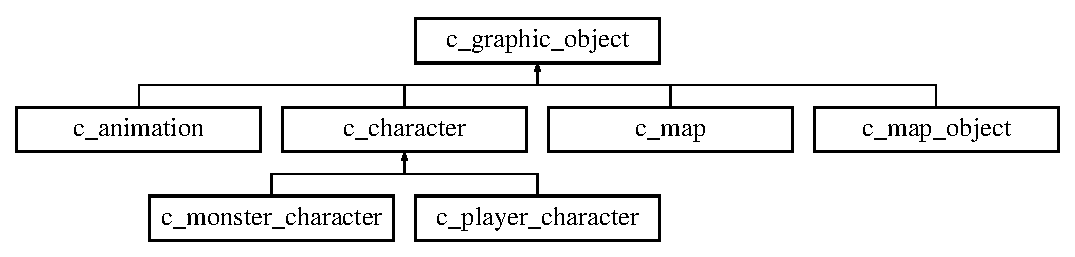
\includegraphics[height=3.000000cm]{classc__graphic__object}
\end{center}
\end{figure}
\subsection*{Public Member Functions}
\begin{DoxyCompactItemize}
\item 
virtual void \hyperlink{classc__graphic__object_a94ef8137eed9ce1ae7adf366fefb51cf}{draw} (int x, int y)
\item 
virtual void \hyperlink{classc__graphic__object_aa87323c0df1b2e79cef78573b6096512}{play\-\_\-animation} (t\-\_\-animation\-\_\-type animation)
\item 
virtual void \hyperlink{classc__graphic__object_ac60b00df5a7edefe4c61e6a59802473f}{loop\-\_\-animation} (t\-\_\-animation\-\_\-type animation)
\item 
virtual void \hyperlink{classc__graphic__object_a32cdba2150d09d903f6e95f2509b9283}{stop\-\_\-animation} ()
\item 
bool \hyperlink{classc__graphic__object_af5f3b289e5f0f4501ee5b5a36fb4aad8}{is\-\_\-animating} ()
\item 
virtual void \hyperlink{classc__graphic__object_a20fa3f61532b73f64f3307fd14b7dba6}{update\-\_\-animation\-\_\-period} ()
\item 
t\-\_\-animation\-\_\-type \hyperlink{classc__graphic__object_a3028097b164e7d88fbde871af2bcc679}{get\-\_\-playing\-\_\-animation} ()
\item 
bool \hyperlink{classc__graphic__object_aef3311c6cff7e455867882eba8b34e84}{is\-\_\-succesfully\-\_\-loaded} ()
\item 
int \hyperlink{classc__graphic__object_a8e692d099d44b9d367d197bc2a582d16}{get\-\_\-animation\-\_\-frame} ()
\end{DoxyCompactItemize}
\subsection*{Protected Attributes}
\begin{DoxyCompactItemize}
\item 
t\-\_\-animation\-\_\-type \hyperlink{classc__graphic__object_a3633db416c2709f2f65a858de7a2d9ae}{playing\-\_\-animation}
\item 
long int \hyperlink{classc__graphic__object_a48b5ab1a193f296ead7119461a4e425e}{started\-\_\-playing}
\item 
long int $\ast$ \hyperlink{classc__graphic__object_a9ff91aa7a60272a8f713ff011a0cc0bb}{global\-\_\-time}
\item 
long int \hyperlink{classc__graphic__object_a327008d33c50fe3665514770eaaaeb11}{animation\-\_\-frame}
\item 
bool \hyperlink{classc__graphic__object_a9b4e51cd726799f6d6902e1759719bbc}{looping\-\_\-animation}
\item 
int \hyperlink{classc__graphic__object_a20a3a703402913137adead51faa53e79}{animation\-\_\-period}
\item 
bool \hyperlink{classc__graphic__object_ad1d6ffa4b597a667995ec1e8c930a9f9}{succesfully\-\_\-loaded}
\item 
bool \hyperlink{classc__graphic__object_a3994cab2b5b4fe62ca0c5b1bc2e03460}{playing\-\_\-sound}
\item 
double \hyperlink{classc__graphic__object_a8274f6e9f1221b91be61ca923e1dc03c}{sound\-\_\-gain}
\item 
A\-L\-L\-E\-G\-R\-O\-\_\-\-S\-A\-M\-P\-L\-E\-\_\-\-I\-D \hyperlink{classc__graphic__object_abf8bc08bd583d2fd1209eba2ae0fdebf}{playing\-\_\-sound\-\_\-id}
\item 
A\-L\-L\-E\-G\-R\-O\-\_\-\-S\-A\-M\-P\-L\-E $\ast$ \hyperlink{classc__graphic__object_a4076fe5b3cd2e8bcb249f54fb86d662f}{sound}
\end{DoxyCompactItemize}


\subsection{Member Function Documentation}
\hypertarget{classc__graphic__object_a94ef8137eed9ce1ae7adf366fefb51cf}{\index{c\-\_\-graphic\-\_\-object@{c\-\_\-graphic\-\_\-object}!draw@{draw}}
\index{draw@{draw}!c_graphic_object@{c\-\_\-graphic\-\_\-object}}
\subsubsection[{draw}]{\setlength{\rightskip}{0pt plus 5cm}void c\-\_\-graphic\-\_\-object\-::draw (
\begin{DoxyParamCaption}
\item[{int}]{x, }
\item[{int}]{y}
\end{DoxyParamCaption}
)\hspace{0.3cm}{\ttfamily [virtual]}}}\label{classc__graphic__object_a94ef8137eed9ce1ae7adf366fefb51cf}
sound played during animation

Graphic object class implementation.

authors\-: Miloslav Číž year\-: 2013 

Reimplemented in \hyperlink{classc__map_a46afcfac9b83f37a28a5cf3e1da91ef6}{c\-\_\-map}, \hyperlink{classc__map__object_add8a45bcf4f77ba65716095c05483f4f}{c\-\_\-map\-\_\-object}, \hyperlink{classc__monster__character_ac400987c335adde2454cab352a63d3d2}{c\-\_\-monster\-\_\-character}, \hyperlink{classc__animation_a36d69237de6781450680a38717385721}{c\-\_\-animation}, and \hyperlink{classc__player__character_a75d0ecbf8d1892422766f4f46ace576e}{c\-\_\-player\-\_\-character}.

\hypertarget{classc__graphic__object_a8e692d099d44b9d367d197bc2a582d16}{\index{c\-\_\-graphic\-\_\-object@{c\-\_\-graphic\-\_\-object}!get\-\_\-animation\-\_\-frame@{get\-\_\-animation\-\_\-frame}}
\index{get\-\_\-animation\-\_\-frame@{get\-\_\-animation\-\_\-frame}!c_graphic_object@{c\-\_\-graphic\-\_\-object}}
\subsubsection[{get\-\_\-animation\-\_\-frame}]{\setlength{\rightskip}{0pt plus 5cm}int c\-\_\-graphic\-\_\-object\-::get\-\_\-animation\-\_\-frame (
\begin{DoxyParamCaption}
{}
\end{DoxyParamCaption}
)}}\label{classc__graphic__object_a8e692d099d44b9d367d197bc2a582d16}
Checks if the map has been loaded succesfully.

\begin{DoxyReturn}{Returns}
true if the map is loaded succesfully, false otherwise 
\end{DoxyReturn}
\hypertarget{classc__graphic__object_a3028097b164e7d88fbde871af2bcc679}{\index{c\-\_\-graphic\-\_\-object@{c\-\_\-graphic\-\_\-object}!get\-\_\-playing\-\_\-animation@{get\-\_\-playing\-\_\-animation}}
\index{get\-\_\-playing\-\_\-animation@{get\-\_\-playing\-\_\-animation}!c_graphic_object@{c\-\_\-graphic\-\_\-object}}
\subsubsection[{get\-\_\-playing\-\_\-animation}]{\setlength{\rightskip}{0pt plus 5cm}t\-\_\-animation\-\_\-type c\-\_\-graphic\-\_\-object\-::get\-\_\-playing\-\_\-animation (
\begin{DoxyParamCaption}
{}
\end{DoxyParamCaption}
)}}\label{classc__graphic__object_a3028097b164e7d88fbde871af2bcc679}
Depending on current animation sets the animation period attribute. \hypertarget{classc__graphic__object_af5f3b289e5f0f4501ee5b5a36fb4aad8}{\index{c\-\_\-graphic\-\_\-object@{c\-\_\-graphic\-\_\-object}!is\-\_\-animating@{is\-\_\-animating}}
\index{is\-\_\-animating@{is\-\_\-animating}!c_graphic_object@{c\-\_\-graphic\-\_\-object}}
\subsubsection[{is\-\_\-animating}]{\setlength{\rightskip}{0pt plus 5cm}bool c\-\_\-graphic\-\_\-object\-::is\-\_\-animating (
\begin{DoxyParamCaption}
{}
\end{DoxyParamCaption}
)}}\label{classc__graphic__object_af5f3b289e5f0f4501ee5b5a36fb4aad8}
Stops playing the current animation. \hypertarget{classc__graphic__object_aef3311c6cff7e455867882eba8b34e84}{\index{c\-\_\-graphic\-\_\-object@{c\-\_\-graphic\-\_\-object}!is\-\_\-succesfully\-\_\-loaded@{is\-\_\-succesfully\-\_\-loaded}}
\index{is\-\_\-succesfully\-\_\-loaded@{is\-\_\-succesfully\-\_\-loaded}!c_graphic_object@{c\-\_\-graphic\-\_\-object}}
\subsubsection[{is\-\_\-succesfully\-\_\-loaded}]{\setlength{\rightskip}{0pt plus 5cm}bool c\-\_\-graphic\-\_\-object\-::is\-\_\-succesfully\-\_\-loaded (
\begin{DoxyParamCaption}
{}
\end{DoxyParamCaption}
)}}\label{classc__graphic__object_aef3311c6cff7e455867882eba8b34e84}
Returns a type of animation being played or looped.

\begin{DoxyReturn}{Returns}
type of animation 
\end{DoxyReturn}
\hypertarget{classc__graphic__object_ac60b00df5a7edefe4c61e6a59802473f}{\index{c\-\_\-graphic\-\_\-object@{c\-\_\-graphic\-\_\-object}!loop\-\_\-animation@{loop\-\_\-animation}}
\index{loop\-\_\-animation@{loop\-\_\-animation}!c_graphic_object@{c\-\_\-graphic\-\_\-object}}
\subsubsection[{loop\-\_\-animation}]{\setlength{\rightskip}{0pt plus 5cm}void c\-\_\-graphic\-\_\-object\-::loop\-\_\-animation (
\begin{DoxyParamCaption}
\item[{t\-\_\-animation\-\_\-type}]{animation}
\end{DoxyParamCaption}
)\hspace{0.3cm}{\ttfamily [virtual]}}}\label{classc__graphic__object_ac60b00df5a7edefe4c61e6a59802473f}
Plays given animation.


\begin{DoxyParams}{Parameters}
{\em animation} & animation to be played \\
\hline
\end{DoxyParams}


Reimplemented in \hyperlink{classc__character_a323dd6b7cf6635a0b61e4351178d7518}{c\-\_\-character}.

\hypertarget{classc__graphic__object_aa87323c0df1b2e79cef78573b6096512}{\index{c\-\_\-graphic\-\_\-object@{c\-\_\-graphic\-\_\-object}!play\-\_\-animation@{play\-\_\-animation}}
\index{play\-\_\-animation@{play\-\_\-animation}!c_graphic_object@{c\-\_\-graphic\-\_\-object}}
\subsubsection[{play\-\_\-animation}]{\setlength{\rightskip}{0pt plus 5cm}void c\-\_\-graphic\-\_\-object\-::play\-\_\-animation (
\begin{DoxyParamCaption}
\item[{t\-\_\-animation\-\_\-type}]{animation}
\end{DoxyParamCaption}
)\hspace{0.3cm}{\ttfamily [virtual]}}}\label{classc__graphic__object_aa87323c0df1b2e79cef78573b6096512}
Tells the object to draw itself at given coordinations on the screen.


\begin{DoxyParams}{Parameters}
{\em x} & x coordination of the screen \\
\hline
{\em y} & y coordination of the screen \\
\hline
\end{DoxyParams}


Reimplemented in \hyperlink{classc__player__character_a6fd0d6503cd56998a4e2c8eb8695767b}{c\-\_\-player\-\_\-character}.

\hypertarget{classc__graphic__object_a32cdba2150d09d903f6e95f2509b9283}{\index{c\-\_\-graphic\-\_\-object@{c\-\_\-graphic\-\_\-object}!stop\-\_\-animation@{stop\-\_\-animation}}
\index{stop\-\_\-animation@{stop\-\_\-animation}!c_graphic_object@{c\-\_\-graphic\-\_\-object}}
\subsubsection[{stop\-\_\-animation}]{\setlength{\rightskip}{0pt plus 5cm}void c\-\_\-graphic\-\_\-object\-::stop\-\_\-animation (
\begin{DoxyParamCaption}
{}
\end{DoxyParamCaption}
)\hspace{0.3cm}{\ttfamily [virtual]}}}\label{classc__graphic__object_a32cdba2150d09d903f6e95f2509b9283}
Loops the given animation untill it's stopped by \hyperlink{classc__graphic__object_a32cdba2150d09d903f6e95f2509b9283}{stop\-\_\-animation()}.


\begin{DoxyParams}{Parameters}
{\em animation} & animation to be looped \\
\hline
\end{DoxyParams}
\hypertarget{classc__graphic__object_a20fa3f61532b73f64f3307fd14b7dba6}{\index{c\-\_\-graphic\-\_\-object@{c\-\_\-graphic\-\_\-object}!update\-\_\-animation\-\_\-period@{update\-\_\-animation\-\_\-period}}
\index{update\-\_\-animation\-\_\-period@{update\-\_\-animation\-\_\-period}!c_graphic_object@{c\-\_\-graphic\-\_\-object}}
\subsubsection[{update\-\_\-animation\-\_\-period}]{\setlength{\rightskip}{0pt plus 5cm}void c\-\_\-graphic\-\_\-object\-::update\-\_\-animation\-\_\-period (
\begin{DoxyParamCaption}
{}
\end{DoxyParamCaption}
)\hspace{0.3cm}{\ttfamily [virtual]}}}\label{classc__graphic__object_a20fa3f61532b73f64f3307fd14b7dba6}
Checks if any animation is playing.

\begin{DoxyReturn}{Returns}
true if any animation is playing or looping, false otherwise 
\end{DoxyReturn}


Reimplemented in \hyperlink{classc__map__object_a2df801781fdad9a4b42a78ff5b9c8558}{c\-\_\-map\-\_\-object}, and \hyperlink{classc__player__character_aa5d59edcb370d29b83ac0b2659ab0385}{c\-\_\-player\-\_\-character}.



\subsection{Member Data Documentation}
\hypertarget{classc__graphic__object_a327008d33c50fe3665514770eaaaeb11}{\index{c\-\_\-graphic\-\_\-object@{c\-\_\-graphic\-\_\-object}!animation\-\_\-frame@{animation\-\_\-frame}}
\index{animation\-\_\-frame@{animation\-\_\-frame}!c_graphic_object@{c\-\_\-graphic\-\_\-object}}
\subsubsection[{animation\-\_\-frame}]{\setlength{\rightskip}{0pt plus 5cm}long int c\-\_\-graphic\-\_\-object\-::animation\-\_\-frame\hspace{0.3cm}{\ttfamily [protected]}}}\label{classc__graphic__object_a327008d33c50fe3665514770eaaaeb11}
reference to a global time counter variable (for animations) \hypertarget{classc__graphic__object_a20a3a703402913137adead51faa53e79}{\index{c\-\_\-graphic\-\_\-object@{c\-\_\-graphic\-\_\-object}!animation\-\_\-period@{animation\-\_\-period}}
\index{animation\-\_\-period@{animation\-\_\-period}!c_graphic_object@{c\-\_\-graphic\-\_\-object}}
\subsubsection[{animation\-\_\-period}]{\setlength{\rightskip}{0pt plus 5cm}int c\-\_\-graphic\-\_\-object\-::animation\-\_\-period\hspace{0.3cm}{\ttfamily [protected]}}}\label{classc__graphic__object_a20a3a703402913137adead51faa53e79}
true if the animation is looping, false otherwise \hypertarget{classc__graphic__object_a9ff91aa7a60272a8f713ff011a0cc0bb}{\index{c\-\_\-graphic\-\_\-object@{c\-\_\-graphic\-\_\-object}!global\-\_\-time@{global\-\_\-time}}
\index{global\-\_\-time@{global\-\_\-time}!c_graphic_object@{c\-\_\-graphic\-\_\-object}}
\subsubsection[{global\-\_\-time}]{\setlength{\rightskip}{0pt plus 5cm}long int$\ast$ c\-\_\-graphic\-\_\-object\-::global\-\_\-time\hspace{0.3cm}{\ttfamily [protected]}}}\label{classc__graphic__object_a9ff91aa7a60272a8f713ff011a0cc0bb}
time when the animation started playing to count the animation frame \hypertarget{classc__graphic__object_a9b4e51cd726799f6d6902e1759719bbc}{\index{c\-\_\-graphic\-\_\-object@{c\-\_\-graphic\-\_\-object}!looping\-\_\-animation@{looping\-\_\-animation}}
\index{looping\-\_\-animation@{looping\-\_\-animation}!c_graphic_object@{c\-\_\-graphic\-\_\-object}}
\subsubsection[{looping\-\_\-animation}]{\setlength{\rightskip}{0pt plus 5cm}bool c\-\_\-graphic\-\_\-object\-::looping\-\_\-animation\hspace{0.3cm}{\ttfamily [protected]}}}\label{classc__graphic__object_a9b4e51cd726799f6d6902e1759719bbc}
current animation frame \hypertarget{classc__graphic__object_a3633db416c2709f2f65a858de7a2d9ae}{\index{c\-\_\-graphic\-\_\-object@{c\-\_\-graphic\-\_\-object}!playing\-\_\-animation@{playing\-\_\-animation}}
\index{playing\-\_\-animation@{playing\-\_\-animation}!c_graphic_object@{c\-\_\-graphic\-\_\-object}}
\subsubsection[{playing\-\_\-animation}]{\setlength{\rightskip}{0pt plus 5cm}t\-\_\-animation\-\_\-type c\-\_\-graphic\-\_\-object\-::playing\-\_\-animation\hspace{0.3cm}{\ttfamily [protected]}}}\label{classc__graphic__object_a3633db416c2709f2f65a858de7a2d9ae}
This class represents an object that is able to draw itself on the screen. It can also play animations. \hypertarget{classc__graphic__object_a3994cab2b5b4fe62ca0c5b1bc2e03460}{\index{c\-\_\-graphic\-\_\-object@{c\-\_\-graphic\-\_\-object}!playing\-\_\-sound@{playing\-\_\-sound}}
\index{playing\-\_\-sound@{playing\-\_\-sound}!c_graphic_object@{c\-\_\-graphic\-\_\-object}}
\subsubsection[{playing\-\_\-sound}]{\setlength{\rightskip}{0pt plus 5cm}bool c\-\_\-graphic\-\_\-object\-::playing\-\_\-sound\hspace{0.3cm}{\ttfamily [protected]}}}\label{classc__graphic__object_a3994cab2b5b4fe62ca0c5b1bc2e03460}
stores information about errors \hypertarget{classc__graphic__object_abf8bc08bd583d2fd1209eba2ae0fdebf}{\index{c\-\_\-graphic\-\_\-object@{c\-\_\-graphic\-\_\-object}!playing\-\_\-sound\-\_\-id@{playing\-\_\-sound\-\_\-id}}
\index{playing\-\_\-sound\-\_\-id@{playing\-\_\-sound\-\_\-id}!c_graphic_object@{c\-\_\-graphic\-\_\-object}}
\subsubsection[{playing\-\_\-sound\-\_\-id}]{\setlength{\rightskip}{0pt plus 5cm}A\-L\-L\-E\-G\-R\-O\-\_\-\-S\-A\-M\-P\-L\-E\-\_\-\-I\-D c\-\_\-graphic\-\_\-object\-::playing\-\_\-sound\-\_\-id\hspace{0.3cm}{\ttfamily [protected]}}}\label{classc__graphic__object_abf8bc08bd583d2fd1209eba2ae0fdebf}
sound gain \hypertarget{classc__graphic__object_a4076fe5b3cd2e8bcb249f54fb86d662f}{\index{c\-\_\-graphic\-\_\-object@{c\-\_\-graphic\-\_\-object}!sound@{sound}}
\index{sound@{sound}!c_graphic_object@{c\-\_\-graphic\-\_\-object}}
\subsubsection[{sound}]{\setlength{\rightskip}{0pt plus 5cm}A\-L\-L\-E\-G\-R\-O\-\_\-\-S\-A\-M\-P\-L\-E$\ast$ c\-\_\-graphic\-\_\-object\-::sound\hspace{0.3cm}{\ttfamily [protected]}}}\label{classc__graphic__object_a4076fe5b3cd2e8bcb249f54fb86d662f}
an I\-D of the sound being played \hypertarget{classc__graphic__object_a8274f6e9f1221b91be61ca923e1dc03c}{\index{c\-\_\-graphic\-\_\-object@{c\-\_\-graphic\-\_\-object}!sound\-\_\-gain@{sound\-\_\-gain}}
\index{sound\-\_\-gain@{sound\-\_\-gain}!c_graphic_object@{c\-\_\-graphic\-\_\-object}}
\subsubsection[{sound\-\_\-gain}]{\setlength{\rightskip}{0pt plus 5cm}double c\-\_\-graphic\-\_\-object\-::sound\-\_\-gain\hspace{0.3cm}{\ttfamily [protected]}}}\label{classc__graphic__object_a8274f6e9f1221b91be61ca923e1dc03c}
whether a sound is playing for this object \hypertarget{classc__graphic__object_a48b5ab1a193f296ead7119461a4e425e}{\index{c\-\_\-graphic\-\_\-object@{c\-\_\-graphic\-\_\-object}!started\-\_\-playing@{started\-\_\-playing}}
\index{started\-\_\-playing@{started\-\_\-playing}!c_graphic_object@{c\-\_\-graphic\-\_\-object}}
\subsubsection[{started\-\_\-playing}]{\setlength{\rightskip}{0pt plus 5cm}long int c\-\_\-graphic\-\_\-object\-::started\-\_\-playing\hspace{0.3cm}{\ttfamily [protected]}}}\label{classc__graphic__object_a48b5ab1a193f296ead7119461a4e425e}
type of animation being played or looped \hypertarget{classc__graphic__object_ad1d6ffa4b597a667995ec1e8c930a9f9}{\index{c\-\_\-graphic\-\_\-object@{c\-\_\-graphic\-\_\-object}!succesfully\-\_\-loaded@{succesfully\-\_\-loaded}}
\index{succesfully\-\_\-loaded@{succesfully\-\_\-loaded}!c_graphic_object@{c\-\_\-graphic\-\_\-object}}
\subsubsection[{succesfully\-\_\-loaded}]{\setlength{\rightskip}{0pt plus 5cm}bool c\-\_\-graphic\-\_\-object\-::succesfully\-\_\-loaded\hspace{0.3cm}{\ttfamily [protected]}}}\label{classc__graphic__object_ad1d6ffa4b597a667995ec1e8c930a9f9}
number of frames of the current animation 

The documentation for this class was generated from the following files\-:\begin{DoxyCompactItemize}
\item 
magerage/graphic\-\_\-object.\-h\item 
magerage/graphic\-\_\-object.\-cpp\end{DoxyCompactItemize}

\hypertarget{classc__map}{\section{c\-\_\-map Class Reference}
\label{classc__map}\index{c\-\_\-map@{c\-\_\-map}}
}
Inheritance diagram for c\-\_\-map\-:\begin{figure}[H]
\begin{center}
\leavevmode
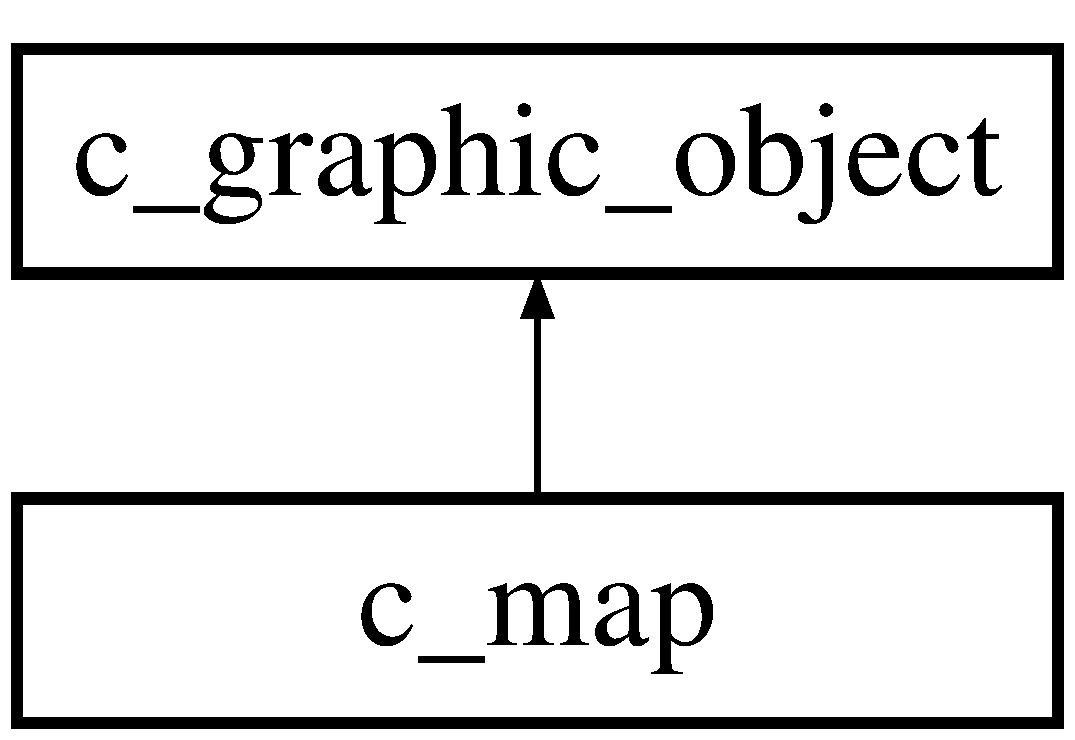
\includegraphics[height=2.000000cm]{classc__map}
\end{center}
\end{figure}
\subsection*{Public Member Functions}
\begin{DoxyCompactItemize}
\item 
\hyperlink{classc__map_a93f9dfae5ef4afdb1b37ee4d31dab1ce}{c\-\_\-map} (string filename, \hyperlink{structt__input__output__state}{t\-\_\-input\-\_\-output\-\_\-state} $\ast$\hyperlink{classc__map_a548cfcecd3a9981dc3c4dd950ceaeab4}{input\-\_\-output\-\_\-state}, long int $\ast$\hyperlink{classc__graphic__object_a9ff91aa7a60272a8f713ff011a0cc0bb}{global\-\_\-time}, int \hyperlink{classc__map_af60c23046dcafb3b9c4a3e097f9e586e}{language})
\item 
\hyperlink{classc__map_a44b7baccc0fafd64c0ff922d127dfb7a}{$\sim$c\-\_\-map} ()
\item 
t\-\_\-game\-\_\-state \hyperlink{classc__map_afcdeaf89863b1c4c758dbb32d2020a25}{update} ()
\item 
virtual void \hyperlink{classc__map_a46afcfac9b83f37a28a5cf3e1da91ef6}{draw} (int x, int y)
\item 
string \hyperlink{classc__map_add3edd9d671e1e62e66baaed5e98a9e9}{get\-\_\-description} ()
\item 
string \hyperlink{classc__map_a2e4546cf04d6149b7d55664f62779f71}{get\-\_\-music\-\_\-name} ()
\end{DoxyCompactItemize}
\subsection*{Protected Member Functions}
\begin{DoxyCompactItemize}
\item 
void \hyperlink{classc__map_a56abddfd11fc1bc9fd9067ad449f21af}{move\-\_\-character} (\hyperlink{classc__character}{c\-\_\-character} $\ast$character, t\-\_\-direction direction)
\item 
void \hyperlink{classc__map_a405354857d0db95dcaf5d4f7371148cb}{add\-\_\-map\-\_\-object} (\hyperlink{classc__map__object}{c\-\_\-map\-\_\-object} $\ast$map\-\_\-object, int x, int y)
\item 
void \hyperlink{classc__map_aeff67cce172a9d464917ccccd03eab47}{use\-\_\-key\-\_\-press} ()
\item 
void \hyperlink{classc__map_a3ea565ef763bd3aaa610d1ab21f72068}{cast\-\_\-key\-\_\-press} (int spell\-\_\-number)
\item 
bool \hyperlink{classc__map_a97ea01c33b55d2e3d1d706f39aa24588}{load\-\_\-from\-\_\-file} (string filename)
\item 
bool \hyperlink{classc__map_a37968729cca9219336b7f31265f3fc40}{character\-\_\-can\-\_\-move\-\_\-to\-\_\-square} (\hyperlink{classc__character}{c\-\_\-character} $\ast$character, t\-\_\-direction direction)
\item 
bool \hyperlink{classc__map_aab9ab7a3336fd65506e5c842a2d217f1}{square\-\_\-has\-\_\-object} (int x, int y, t\-\_\-object\-\_\-type object\-\_\-type)
\item 
bool \hyperlink{classc__map_af4970a07daeff76db0cc32b6b69a93c9}{square\-\_\-is\-\_\-stepable} (int x, int y)
\item 
int \hyperlink{classc__map_a790027eaa0b60bcd2a11801e961a5232}{get\-\_\-elevation\-\_\-for\-\_\-character} (\hyperlink{classc__character}{c\-\_\-character} $\ast$character)
\item 
bool \hyperlink{classc__map_a24ac92070725adc1c295246887df88a1}{set\-\_\-environment} (t\-\_\-environment new\-\_\-environment)
\item 
int \hyperlink{classc__map_a250c11079b911dc753bc5dcb9521813e}{get\-\_\-height} (int x, int y)
\item 
int \hyperlink{classc__map_a273cb97d6d816e839a42460af56152f6}{get\-\_\-terrain\-\_\-height} (int x, int y)
\item 
void \hyperlink{classc__map_af929a9ab4f0d6cd50e58ac8956afa846}{shift\-\_\-crate} (int x, int y, t\-\_\-direction direction)
\item 
bool \hyperlink{classc__map_a7ed031ff3dbd23f042273180f5f0abfb}{crate\-\_\-can\-\_\-be\-\_\-shifted} (int x, int y, int \hyperlink{classc__map_af30ddc07f94cbc2e9c91cbdfd3f68cc5}{height}, t\-\_\-direction direction)
\item 
t\-\_\-square\-\_\-type \hyperlink{classc__map_a876a3d275b3d88e3106d7af62c823774}{get\-\_\-square\-\_\-type} (int x, int y)
\item 
void \hyperlink{classc__map_a2d6baf17ed853fc872da4adafe956426}{set\-\_\-square\-\_\-type} (int x, int y, t\-\_\-square\-\_\-type type)
\item 
void \hyperlink{classc__map_a3c30d1f9254e0aeb71e2859d7e879e72}{update\-\_\-map\-\_\-object\-\_\-states} ()
\item 
void \hyperlink{classc__map_a4033258ab06d0867efb3cf534cf8b93f}{remove\-\_\-object} (int x, int y, int index)
\item 
void \hyperlink{classc__map_ae840e8935d33f10baf479a4ff7f10c27}{link\-\_\-objects} ()
\item 
void \hyperlink{classc__map_ad0732462db74b1bc531196b2d1247809}{check\-\_\-buttons} ()
\item 
void \hyperlink{classc__map_a64d2a8dd8dd79eb92c6ff2d087907369}{draw\-\_\-borders} (int x, int y, int plus\-\_\-x, int plus\-\_\-y)
\item 
bool \hyperlink{classc__map_a798709905b72d00d95940b78e5c7cabc}{must\-\_\-have\-\_\-border} (t\-\_\-square\-\_\-type type1, t\-\_\-square\-\_\-type type2)
\item 
bool \hyperlink{classc__map_a0a382a09197490bc1557bf64745db261}{square\-\_\-has\-\_\-character} (int x, int y)
\item 
void \hyperlink{classc__map_a1a60a7de987db9e2dd88672f19890cb3}{display\-\_\-animation} (t\-\_\-display\-\_\-animation animation, int x, int y)
\item 
void \hyperlink{classc__map_a706ea8f6dffb4881bee80f97e12d611b}{update\-\_\-screen\-\_\-position} ()
\item 
void \hyperlink{classc__map_ac589863287ad3ab09d3766f39da6fd09}{fire\-\_\-missile} (int spell\-\_\-number)
\item 
void \hyperlink{classc__map_a0a72be4c098a468e7c3737230027eb4d}{update\-\_\-missiles} ()
\item 
void \hyperlink{classc__map_afd7f4e6c58a622b83580d236397530a3}{switch\-\_\-player} (int player\-\_\-number)
\item 
void \hyperlink{classc__map_a0f0fdbcf0a83552527eae22a098b6fd4}{update\-\_\-flames} ()
\item 
bool \hyperlink{classc__map_a0ed756d1637812842f65138042333d50}{object\-\_\-can\-\_\-be\-\_\-used} (\hyperlink{classc__map__object}{c\-\_\-map\-\_\-object} $\ast$what)
\item 
void \hyperlink{classc__map_a1f90f7d0ebe3228203f68bb3af4be5f0}{get\-\_\-object\-\_\-position} (\hyperlink{classc__map__object}{c\-\_\-map\-\_\-object} $\ast$what, int $\ast$x, int $\ast$y)
\item 
void \hyperlink{classc__map_a4abaca91d31f0eb0fea80c48533f578e}{display\-\_\-text} (string text, double duration)
\item 
void \hyperlink{classc__map_a3a2279cfc3ee5a721073b5b29fcf8e56}{check\-\_\-teleport} ()
\item 
bool \hyperlink{classc__map_ac53831c7f1f8fe285f6dbbc3968ede9c}{door\-\_\-can\-\_\-be\-\_\-passed} (int x, int y, t\-\_\-direction direction)
\item 
void \hyperlink{classc__map_a8cec3eb1eb4d72536aa2c1d9209ca23b}{update\-\_\-monsters} ()
\item 
void \hyperlink{classc__map_aae5774997458b6cd01bebf5ba7578716}{shift\-\_\-screen} (int x, int y)
\item 
void \hyperlink{classc__map_a42f4ffc135ca44bf92e93d3915bee769}{check\-\_\-ice} ()
\item 
void \hyperlink{classc__map_ad1f16a723dfbc854557827b207f7f44a}{set\-\_\-map\-\_\-objects} (string object\-\_\-string)
\item 
void \hyperlink{classc__map_afbef00c25eed696050c8e0fc11c770d5}{set\-\_\-monsters} (string monster\-\_\-string)
\item 
void \hyperlink{classc__map_a1caec6390a6a85a5d98bbb0c89e3ff31}{record\-\_\-buttons} ()
\item 
t\-\_\-game\-\_\-state \hyperlink{classc__map_a6fe5b03607efeac17bca71a27f1767c3}{check\-\_\-game\-\_\-state} ()
\end{DoxyCompactItemize}
\subsection*{Static Protected Member Functions}
\begin{DoxyCompactItemize}
\item 
static void \hyperlink{classc__map_a882c99e5b3a1ce62f68b65dc74be5c62}{next\-\_\-square} (int x, int y, t\-\_\-direction direction, int $\ast$next\-\_\-x, int $\ast$next\-\_\-y)
\item 
static string \hyperlink{classc__map_a1cae0c68558c2830c8775528d7cb0425}{get\-\_\-nth\-\_\-substring} (string from\-\_\-what, int n)
\end{DoxyCompactItemize}
\subsection*{Protected Attributes}
\begin{DoxyCompactItemize}
\item 
int \hyperlink{classc__map_a24f23160d66e61d5f6943cd4f51aa06f}{width}
\item 
int \hyperlink{classc__map_af30ddc07f94cbc2e9c91cbdfd3f68cc5}{height}
\item 
int $\ast$ \hyperlink{classc__map_a4d9edbbf1f0e9465f7e04307af02afab}{button\-\_\-positions\-\_\-x}
\item 
int $\ast$ \hyperlink{classc__map_a6be0ac983d8dfd2aa801face76908dff}{button\-\_\-positions\-\_\-y}
\item 
int \hyperlink{classc__map_af36d349e1b651e72551f361b88cb9a76}{number\-\_\-of\-\_\-buttons}
\item 
int \hyperlink{classc__map_aee9ff4ca6cc941590f843b7c88b50067}{current\-\_\-player}
\item 
int \hyperlink{classc__map_a1fb9429d0318c721540dbe6337615cff}{screen\-\_\-center\-\_\-x}
\item 
int \hyperlink{classc__map_a060e812813124210995493d10bc873d0}{screen\-\_\-center\-\_\-y}
\item 
t\-\_\-environment \hyperlink{classc__map_a7717281184aa1c3eca2d1b2377a16d9d}{environment}
\item 
\hyperlink{structt__map__square}{t\-\_\-map\-\_\-square} \hyperlink{classc__map_ad2884dc5a43ee568bad98b47f8eebef5}{squares} \mbox{[}M\-A\-P\-\_\-\-M\-A\-X\-\_\-\-W\-I\-D\-T\-H\mbox{]}\mbox{[}M\-A\-P\-\_\-\-M\-A\-X\-\_\-\-H\-E\-I\-G\-H\-T\mbox{]}
\item 
\hyperlink{classc__player__character}{c\-\_\-player\-\_\-character} $\ast$ \hyperlink{classc__map_a54131ed05249666c5ba32558a1df7d3e}{player\-\_\-characters} \mbox{[}3\mbox{]}
\item 
\hyperlink{classc__monster__character}{c\-\_\-monster\-\_\-character} $\ast$ \hyperlink{classc__map_af0168711e28d3671a9ef69003f3f0dc6}{monster\-\_\-characters} \mbox{[}M\-A\-X\-\_\-\-M\-O\-N\-S\-T\-E\-R\-S\-\_\-\-O\-N\-\_\-\-M\-A\-P\mbox{]}
\item 
int \hyperlink{classc__map_aab102e2ce55754d739b6679740f97a7c}{number\-\_\-of\-\_\-monsters}
\item 
\hyperlink{structt__input__output__state}{t\-\_\-input\-\_\-output\-\_\-state} $\ast$ \hyperlink{classc__map_a548cfcecd3a9981dc3c4dd950ceaeab4}{input\-\_\-output\-\_\-state}
\item 
double \hyperlink{classc__map_ab59ec9afe1f17edc59308fe5392b99bd}{time\-\_\-before}
\item 
double \hyperlink{classc__map_a7a1d7aaf2dafa841ec84f9b6aa256b5b}{time\-\_\-difference}
\item 
int \hyperlink{classc__map_aeb595cd9e54fd327225d36119f128496}{portrait\-\_\-x\-\_\-positions} \mbox{[}3\mbox{]}
\item 
int \hyperlink{classc__map_abd86f152d66885aa67f8ec22ac4b3bca}{portrait\-\_\-y\-\_\-position}
\item 
bool \hyperlink{classc__map_a05a4919684f8a4d6c10342f4e8231124}{pressed\-\_\-1}
\item 
bool \hyperlink{classc__map_a0d69618264aff3f1b167d4fc3bb5ceb3}{pressed\-\_\-2}
\item 
\hypertarget{classc__map_abdf89ab0f7c6595c01f70276dbaefc32}{bool {\bfseries pressed\-\_\-3}}\label{classc__map_abdf89ab0f7c6595c01f70276dbaefc32}

\item 
\hypertarget{classc__map_af7479a56bab6a7b49c8c89bae2871605}{bool {\bfseries mouse\-\_\-pressed}}\label{classc__map_af7479a56bab6a7b49c8c89bae2871605}

\item 
\hypertarget{classc__map_ae3e456c5c75e2a280eb56d9a473b82b0}{bool {\bfseries check\-\_\-firecloak}}\label{classc__map_ae3e456c5c75e2a280eb56d9a473b82b0}

\item 
double \hyperlink{classc__map_a38c8548138806d350a13fc6ace496d14}{fire\-\_\-cloak\-\_\-end\-\_\-time}
\item 
int \hyperlink{classc__map_af60c23046dcafb3b9c4a3e097f9e586e}{language}
\item 
int \hyperlink{classc__map_a2c290e7b1d47f8c846fc77aa4464c8e7}{textbox\-\_\-size} \mbox{[}2\mbox{]}
\item 
string \hyperlink{classc__map_ad1b2ee98d03858d529bf35854473ecc6}{description}
\item 
bool \hyperlink{classc__map_af471bb004fc765a15293604a0830bca2}{oren\-\_\-destroyed}
\item 
double \hyperlink{classc__map_af7ac20f46aab8dde2b4459642fd5d3de}{change\-\_\-flame\-\_\-state}
\item 
string \hyperlink{classc__map_aeab133fe9c418a16af900492f8bf49a4}{music\-\_\-name}
\item 
char \hyperlink{classc__map_a97c58015fb3e1e4764d6a522880c5ccf}{text\-\_\-lines} \mbox{[}M\-A\-X\-\_\-\-T\-E\-X\-T\-\_\-\-L\-I\-N\-E\-S\mbox{]}\mbox{[}M\-A\-X\-\_\-\-T\-E\-X\-T\-\_\-\-C\-H\-A\-R\-A\-C\-T\-E\-R\-S\-\_\-\-P\-E\-R\-\_\-\-L\-I\-N\-E\mbox{]}
\item 
bool \hyperlink{classc__map_a6273cd823e9d08f0b277e6407b468ff3}{text\-\_\-is\-\_\-displayed}
\item 
double \hyperlink{classc__map_ad911699c6d1ad83868e75551d138b4e7}{text\-\_\-end\-\_\-time}
\item 
bool \hyperlink{classc__map_a42c18f1bd057c4dcd88ec2de95c854fe}{flames\-\_\-on}
\item 
int \hyperlink{classc__map_ae7f6ee0b7e9f43cf0344d55480595803}{frame\-\_\-count}
\item 
\hyperlink{structt__missile}{t\-\_\-missile} \hyperlink{classc__map_a7a421fc457cc901876cc7e8d0fbc13e8}{missiles} \mbox{[}M\-A\-X\-\_\-\-M\-I\-S\-S\-I\-L\-E\-S\-\_\-\-O\-N\-\_\-\-M\-A\-P\mbox{]}
\item 
int \hyperlink{classc__map_a83302b5feea5bc2e3e9bc10efa23396f}{number\-\_\-of\-\_\-missiles}
\item 
int \hyperlink{classc__map_af760f25a8a9a58ce904ac0f0b3ee6887}{screen\-\_\-square\-\_\-resolution} \mbox{[}2\mbox{]}
\item 
int \hyperlink{classc__map_a2b6fac3ee312a52883ab9ff692dbaf0b}{screen\-\_\-square\-\_\-position} \mbox{[}2\mbox{]}
\item 
int \hyperlink{classc__map_afa78589723b061e99ecfe9f7ae9a5fdd}{screen\-\_\-pixel\-\_\-position} \mbox{[}2\mbox{]}
\item 
int \hyperlink{classc__map_a4fd1b68220337cb514fed398fe79b7ab}{screen\-\_\-square\-\_\-end} \mbox{[}2\mbox{]}
\item 
\hyperlink{classc__animation}{c\-\_\-animation} $\ast$ \hyperlink{classc__map_a777d0b0ec7a0a14c1ccae809cb09f4b1}{animation\-\_\-water\-\_\-splash}
\item 
\hyperlink{classc__animation}{c\-\_\-animation} $\ast$ \hyperlink{classc__map_a27650c86dc14f11dff3d582f3ffd540e}{animation\-\_\-refresh}
\item 
\hyperlink{classc__animation}{c\-\_\-animation} $\ast$ \hyperlink{classc__map_ab18a6618eae74007423595aaa606b15c}{animation\-\_\-crate\-\_\-shift\-\_\-north}
\item 
\hyperlink{classc__animation}{c\-\_\-animation} $\ast$ \hyperlink{classc__map_af34abe429db8bba11ccc582a5c2b0b29}{animation\-\_\-collapse}
\item 
\hyperlink{classc__animation}{c\-\_\-animation} $\ast$ \hyperlink{classc__map_a23a9d2c692bc90f9b78f1274f24378e7}{animation\-\_\-melt}
\item 
\hyperlink{classc__animation}{c\-\_\-animation} $\ast$ \hyperlink{classc__map_a812ca3ddb1f4ff364861a4a4f3318caf}{animation\-\_\-teleport}
\item 
\hyperlink{classc__animation}{c\-\_\-animation} $\ast$ \hyperlink{classc__map_a1be7994a019936dccdf711ca8bfcaba3}{animation\-\_\-explosion}
\item 
\hyperlink{classc__animation}{c\-\_\-animation} $\ast$ \hyperlink{classc__map_ad52da3cd4cd1e0c88ce8170314b09f78}{animation\-\_\-shadow\-\_\-explosion}
\item 
A\-L\-L\-E\-G\-R\-O\-\_\-\-B\-I\-T\-M\-A\-P $\ast$ \hyperlink{classc__map_a297d97b704636559a28596af02cf9f79}{portrait\-\_\-selection}
\item 
A\-L\-L\-E\-G\-R\-O\-\_\-\-B\-I\-T\-M\-A\-P $\ast$ \hyperlink{classc__map_a9816fa208514e89a87693508fa5606ae}{portrait\-\_\-mia}
\item 
A\-L\-L\-E\-G\-R\-O\-\_\-\-B\-I\-T\-M\-A\-P $\ast$ \hyperlink{classc__map_af599cccfc6f1260aa5c1b0a236dca397}{portrait\-\_\-metodej}
\item 
A\-L\-L\-E\-G\-R\-O\-\_\-\-B\-I\-T\-M\-A\-P $\ast$ \hyperlink{classc__map_a9801a871513ce172735eb4afe070f184}{portrait\-\_\-starovous}
\item 
A\-L\-L\-E\-G\-R\-O\-\_\-\-B\-I\-T\-M\-A\-P $\ast$ \hyperlink{classc__map_a928e809cafb17cee55193944f6aafe24}{tile}
\item 
A\-L\-L\-E\-G\-R\-O\-\_\-\-B\-I\-T\-M\-A\-P $\ast$ \hyperlink{classc__map_ab84679456c3df51222049c4fb80d66a9}{tile\-\_\-cliff\-\_\-south\-\_\-1}
\item 
A\-L\-L\-E\-G\-R\-O\-\_\-\-B\-I\-T\-M\-A\-P $\ast$ \hyperlink{classc__map_ae725ccf9eb9daefefdb9b58b00388913}{tile\-\_\-cliff\-\_\-south\-\_\-2}
\item 
A\-L\-L\-E\-G\-R\-O\-\_\-\-B\-I\-T\-M\-A\-P $\ast$ \hyperlink{classc__map_abecd9b0a1aab4c4e02cbe698ddb487ee}{tile\-\_\-cliff\-\_\-southwest\-\_\-1}
\item 
A\-L\-L\-E\-G\-R\-O\-\_\-\-B\-I\-T\-M\-A\-P $\ast$ \hyperlink{classc__map_ae1b595833e6967f8d27fd5a2252d12b3}{tile\-\_\-cliff\-\_\-southwest\-\_\-2}
\item 
A\-L\-L\-E\-G\-R\-O\-\_\-\-B\-I\-T\-M\-A\-P $\ast$ \hyperlink{classc__map_a9d5707e014681a6d16044d483688c081}{tile\-\_\-cliff\-\_\-southeast\-\_\-1}
\item 
A\-L\-L\-E\-G\-R\-O\-\_\-\-B\-I\-T\-M\-A\-P $\ast$ \hyperlink{classc__map_a1aefdb38df373482aff57b9243ec9d67}{tile\-\_\-cliff\-\_\-southeast\-\_\-2}
\item 
A\-L\-L\-E\-G\-R\-O\-\_\-\-B\-I\-T\-M\-A\-P $\ast$ \hyperlink{classc__map_aa40008668fa55a28089cd20c03563926}{tile\-\_\-cliff\-\_\-west}
\item 
A\-L\-L\-E\-G\-R\-O\-\_\-\-B\-I\-T\-M\-A\-P $\ast$ \hyperlink{classc__map_a105d6f1355ca490246a8a5bf56bbe844}{tile\-\_\-cliff\-\_\-east}
\item 
A\-L\-L\-E\-G\-R\-O\-\_\-\-B\-I\-T\-M\-A\-P $\ast$ \hyperlink{classc__map_aa8892af60c621c949f8f46485bd6f8b8}{tile\-\_\-cliff\-\_\-north}
\item 
A\-L\-L\-E\-G\-R\-O\-\_\-\-B\-I\-T\-M\-A\-P $\ast$ \hyperlink{classc__map_aec73bf9c12354078037cc6d1b4de6025}{tile\-\_\-cliff\-\_\-northwest}
\item 
A\-L\-L\-E\-G\-R\-O\-\_\-\-B\-I\-T\-M\-A\-P $\ast$ \hyperlink{classc__map_a1dd3e087030dad02e1329416daaf58bc}{tile\-\_\-cliff\-\_\-northeast}
\item 
A\-L\-L\-E\-G\-R\-O\-\_\-\-B\-I\-T\-M\-A\-P $\ast$ \hyperlink{classc__map_a0ba260cfc9fd354f0b05900b90367cfa}{tile\-\_\-edge}
\item 
A\-L\-L\-E\-G\-R\-O\-\_\-\-B\-I\-T\-M\-A\-P $\ast$ \hyperlink{classc__map_a1d7fc093a6e24ba1ea66b66505ad8581}{tile\-\_\-water} \mbox{[}5\mbox{]}
\item 
A\-L\-L\-E\-G\-R\-O\-\_\-\-B\-I\-T\-M\-A\-P $\ast$ \hyperlink{classc__map_a12e5d9ac851eba093b98998593b7f3a9}{tile\-\_\-ice}
\item 
A\-L\-L\-E\-G\-R\-O\-\_\-\-B\-I\-T\-M\-A\-P $\ast$ \hyperlink{classc__map_ae13539d062f5a9eb89ebf72d7e3890be}{tile\-\_\-collapse}
\item 
A\-L\-L\-E\-G\-R\-O\-\_\-\-B\-I\-T\-M\-A\-P $\ast$ \hyperlink{classc__map_a539c61c09b1a762ef657139f22ebd7c1}{tile\-\_\-hole}
\item 
A\-L\-L\-E\-G\-R\-O\-\_\-\-B\-I\-T\-M\-A\-P $\ast$ \hyperlink{classc__map_a9b6b2ac643bd82db8acf37753e86482b}{bitmap\-\_\-crate\-\_\-water}
\item 
A\-L\-L\-E\-G\-R\-O\-\_\-\-B\-I\-T\-M\-A\-P $\ast$ \hyperlink{classc__map_a6191d8333fa50a672d1cb02957182b7e}{spell\-\_\-mia\-\_\-1} \mbox{[}3\mbox{]}
\item 
A\-L\-L\-E\-G\-R\-O\-\_\-\-B\-I\-T\-M\-A\-P $\ast$ \hyperlink{classc__map_abea93f3e180070e80bb0dc7f061969cb}{spell\-\_\-mia\-\_\-2} \mbox{[}3\mbox{]}
\item 
A\-L\-L\-E\-G\-R\-O\-\_\-\-B\-I\-T\-M\-A\-P $\ast$ \hyperlink{classc__map_a7299ee552482b6917b4aae7f24263392}{spell\-\_\-metodej\-\_\-1} \mbox{[}3\mbox{]}
\item 
A\-L\-L\-E\-G\-R\-O\-\_\-\-B\-I\-T\-M\-A\-P $\ast$ \hyperlink{classc__map_aaa728703ee5b40637e354f26dcb4f136}{spell\-\_\-starovous\-\_\-1} \mbox{[}3\mbox{]}
\item 
A\-L\-L\-E\-G\-R\-O\-\_\-\-B\-I\-T\-M\-A\-P $\ast$ \hyperlink{classc__map_af8e66f5af3e07acfbcf780e21669b1e0}{spell\-\_\-starovous\-\_\-2} \mbox{[}3\mbox{]}
\item 
A\-L\-L\-E\-G\-R\-O\-\_\-\-B\-I\-T\-M\-A\-P $\ast$ \hyperlink{classc__map_afe0fe7415fc6ab78e753dbb95901dee7}{spell\-\_\-icons} \mbox{[}7\mbox{]}
\item 
A\-L\-L\-E\-G\-R\-O\-\_\-\-B\-I\-T\-M\-A\-P $\ast$ \hyperlink{classc__map_a5bf782d167ce72e2a115c4817954b3db}{map\-\_\-shadow\-\_\-north}
\item 
A\-L\-L\-E\-G\-R\-O\-\_\-\-B\-I\-T\-M\-A\-P $\ast$ \hyperlink{classc__map_a0309d1046d20db4eb0bb065d0d4a6201}{map\-\_\-shadow\-\_\-south}
\item 
A\-L\-L\-E\-G\-R\-O\-\_\-\-B\-I\-T\-M\-A\-P $\ast$ \hyperlink{classc__map_aa388806f4a767a2b6732b0ea3cf12e0d}{map\-\_\-shadow\-\_\-east}
\item 
A\-L\-L\-E\-G\-R\-O\-\_\-\-B\-I\-T\-M\-A\-P $\ast$ \hyperlink{classc__map_ad49b7ca28467f986d4b8a2e69ed1e15e}{map\-\_\-shadow\-\_\-west}
\item 
A\-L\-L\-E\-G\-R\-O\-\_\-\-S\-A\-M\-P\-L\-E $\ast$ \hyperlink{classc__map_abb19c6e3c47f8d1182fe746f1e6ccc40}{spell\-\_\-sounds\-\_\-mia} \mbox{[}2\mbox{]}
\item 
A\-L\-L\-E\-G\-R\-O\-\_\-\-S\-A\-M\-P\-L\-E $\ast$ \hyperlink{classc__map_aec438098bd5ded52ab9c831cd19eb629}{spell\-\_\-sounds\-\_\-metodej} \mbox{[}2\mbox{]}
\item 
A\-L\-L\-E\-G\-R\-O\-\_\-\-S\-A\-M\-P\-L\-E $\ast$ \hyperlink{classc__map_ae7b220711fb2815dc1ac925b39fa81ca}{spell\-\_\-sounds\-\_\-starovous} \mbox{[}2\mbox{]}
\item 
A\-L\-L\-E\-G\-R\-O\-\_\-\-S\-A\-M\-P\-L\-E $\ast$ \hyperlink{classc__map_a046d71e73934bf557644cd207facccdf}{change\-\_\-player\-\_\-sound}
\item 
A\-L\-L\-E\-G\-R\-O\-\_\-\-F\-O\-N\-T $\ast$ \hyperlink{classc__map_ada9b97f91338614f93a9a95fdfd7157b}{text\-\_\-font}
\end{DoxyCompactItemize}


\subsection{Constructor \& Destructor Documentation}
\hypertarget{classc__map_a93f9dfae5ef4afdb1b37ee4d31dab1ce}{\index{c\-\_\-map@{c\-\_\-map}!c\-\_\-map@{c\-\_\-map}}
\index{c\-\_\-map@{c\-\_\-map}!c_map@{c\-\_\-map}}
\subsubsection[{c\-\_\-map}]{\setlength{\rightskip}{0pt plus 5cm}c\-\_\-map\-::c\-\_\-map (
\begin{DoxyParamCaption}
\item[{string}]{filename, }
\item[{{\bf t\-\_\-input\-\_\-output\-\_\-state} $\ast$}]{input\-\_\-output\-\_\-state, }
\item[{long int $\ast$}]{global\-\_\-time, }
\item[{int}]{language}
\end{DoxyParamCaption}
)}}\label{classc__map_a93f9dfae5ef4afdb1b37ee4d31dab1ce}
Checks the game state. That means if nothing happens or if the player lost because he's encountered a monster etc.

\begin{DoxyReturn}{Returns}
current game state 
\end{DoxyReturn}
\hypertarget{classc__map_a44b7baccc0fafd64c0ff922d127dfb7a}{\index{c\-\_\-map@{c\-\_\-map}!$\sim$c\-\_\-map@{$\sim$c\-\_\-map}}
\index{$\sim$c\-\_\-map@{$\sim$c\-\_\-map}!c_map@{c\-\_\-map}}
\subsubsection[{$\sim$c\-\_\-map}]{\setlength{\rightskip}{0pt plus 5cm}c\-\_\-map\-::$\sim$c\-\_\-map (
\begin{DoxyParamCaption}
{}
\end{DoxyParamCaption}
)}}\label{classc__map_a44b7baccc0fafd64c0ff922d127dfb7a}
Class constructor, loads new map from given file.


\begin{DoxyParams}{Parameters}
{\em filename} & path to the map file \\
\hline
{\em input\-\_\-output\-\_\-state} & pointer to structure, which will be used to pass information about keyboard and mouse to this object. \\
\hline
{\em global\-\_\-time} & reference to a global time counter variable which is needed for animations \\
\hline
{\em language} & language number, 0 = english, 1 = czech \\
\hline
\end{DoxyParams}


\subsection{Member Function Documentation}
\hypertarget{classc__map_a405354857d0db95dcaf5d4f7371148cb}{\index{c\-\_\-map@{c\-\_\-map}!add\-\_\-map\-\_\-object@{add\-\_\-map\-\_\-object}}
\index{add\-\_\-map\-\_\-object@{add\-\_\-map\-\_\-object}!c_map@{c\-\_\-map}}
\subsubsection[{add\-\_\-map\-\_\-object}]{\setlength{\rightskip}{0pt plus 5cm}void c\-\_\-map\-::add\-\_\-map\-\_\-object (
\begin{DoxyParamCaption}
\item[{{\bf c\-\_\-map\-\_\-object} $\ast$}]{map\-\_\-object, }
\item[{int}]{x, }
\item[{int}]{y}
\end{DoxyParamCaption}
)\hspace{0.3cm}{\ttfamily [protected]}}}\label{classc__map_a405354857d0db95dcaf5d4f7371148cb}
Updates character's movement in given direction and handles colisions and interaction with map objects.


\begin{DoxyParams}{Parameters}
{\em character} & character to be moved \\
\hline
{\em direction} & direction in which the player is moving \\
\hline
\end{DoxyParams}
\hypertarget{classc__map_a3ea565ef763bd3aaa610d1ab21f72068}{\index{c\-\_\-map@{c\-\_\-map}!cast\-\_\-key\-\_\-press@{cast\-\_\-key\-\_\-press}}
\index{cast\-\_\-key\-\_\-press@{cast\-\_\-key\-\_\-press}!c_map@{c\-\_\-map}}
\subsubsection[{cast\-\_\-key\-\_\-press}]{\setlength{\rightskip}{0pt plus 5cm}void c\-\_\-map\-::cast\-\_\-key\-\_\-press (
\begin{DoxyParamCaption}
\item[{int}]{spell\-\_\-number}
\end{DoxyParamCaption}
)\hspace{0.3cm}{\ttfamily [protected]}}}\label{classc__map_a3ea565ef763bd3aaa610d1ab21f72068}
Handles use key press. \hypertarget{classc__map_a37968729cca9219336b7f31265f3fc40}{\index{c\-\_\-map@{c\-\_\-map}!character\-\_\-can\-\_\-move\-\_\-to\-\_\-square@{character\-\_\-can\-\_\-move\-\_\-to\-\_\-square}}
\index{character\-\_\-can\-\_\-move\-\_\-to\-\_\-square@{character\-\_\-can\-\_\-move\-\_\-to\-\_\-square}!c_map@{c\-\_\-map}}
\subsubsection[{character\-\_\-can\-\_\-move\-\_\-to\-\_\-square}]{\setlength{\rightskip}{0pt plus 5cm}bool c\-\_\-map\-::character\-\_\-can\-\_\-move\-\_\-to\-\_\-square (
\begin{DoxyParamCaption}
\item[{{\bf c\-\_\-character} $\ast$}]{character, }
\item[{t\-\_\-direction}]{direction}
\end{DoxyParamCaption}
)\hspace{0.3cm}{\ttfamily [protected]}}}\label{classc__map_a37968729cca9219336b7f31265f3fc40}
Loads the map from given file. Also loads all other things from files like fonts, sounds etc.


\begin{DoxyParams}{Parameters}
{\em filename} & path to the file \\
\hline
\end{DoxyParams}
\begin{DoxyReturn}{Returns}
true if the map was loaded succesfully, otherwise false 
\end{DoxyReturn}
\hypertarget{classc__map_ad0732462db74b1bc531196b2d1247809}{\index{c\-\_\-map@{c\-\_\-map}!check\-\_\-buttons@{check\-\_\-buttons}}
\index{check\-\_\-buttons@{check\-\_\-buttons}!c_map@{c\-\_\-map}}
\subsubsection[{check\-\_\-buttons}]{\setlength{\rightskip}{0pt plus 5cm}void c\-\_\-map\-::check\-\_\-buttons (
\begin{DoxyParamCaption}
{}
\end{DoxyParamCaption}
)\hspace{0.3cm}{\ttfamily [protected]}}}\label{classc__map_ad0732462db74b1bc531196b2d1247809}
Establishes pointer connections between map objects depending on their link ids. \hypertarget{classc__map_a6fe5b03607efeac17bca71a27f1767c3}{\index{c\-\_\-map@{c\-\_\-map}!check\-\_\-game\-\_\-state@{check\-\_\-game\-\_\-state}}
\index{check\-\_\-game\-\_\-state@{check\-\_\-game\-\_\-state}!c_map@{c\-\_\-map}}
\subsubsection[{check\-\_\-game\-\_\-state}]{\setlength{\rightskip}{0pt plus 5cm}t\-\_\-game\-\_\-state c\-\_\-map\-::check\-\_\-game\-\_\-state (
\begin{DoxyParamCaption}
{}
\end{DoxyParamCaption}
)\hspace{0.3cm}{\ttfamily [protected]}}}\label{classc__map_a6fe5b03607efeac17bca71a27f1767c3}
Records all buttons on the map into special data structure so that the checking of them will be faster. This must be called in order for buttons to work. \hypertarget{classc__map_a42f4ffc135ca44bf92e93d3915bee769}{\index{c\-\_\-map@{c\-\_\-map}!check\-\_\-ice@{check\-\_\-ice}}
\index{check\-\_\-ice@{check\-\_\-ice}!c_map@{c\-\_\-map}}
\subsubsection[{check\-\_\-ice}]{\setlength{\rightskip}{0pt plus 5cm}void c\-\_\-map\-::check\-\_\-ice (
\begin{DoxyParamCaption}
{}
\end{DoxyParamCaption}
)\hspace{0.3cm}{\ttfamily [protected]}}}\label{classc__map_a42f4ffc135ca44bf92e93d3915bee769}
Shifts the screen by given values. Checks borders and doesn't allow the screen to be shifted too far.


\begin{DoxyParams}{Parameters}
{\em x} & possibly negative x offset in pixels \\
\hline
{\em y} & possibly negative y offset in pixels \\
\hline
\end{DoxyParams}
\hypertarget{classc__map_a3a2279cfc3ee5a721073b5b29fcf8e56}{\index{c\-\_\-map@{c\-\_\-map}!check\-\_\-teleport@{check\-\_\-teleport}}
\index{check\-\_\-teleport@{check\-\_\-teleport}!c_map@{c\-\_\-map}}
\subsubsection[{check\-\_\-teleport}]{\setlength{\rightskip}{0pt plus 5cm}void c\-\_\-map\-::check\-\_\-teleport (
\begin{DoxyParamCaption}
{}
\end{DoxyParamCaption}
)\hspace{0.3cm}{\ttfamily [protected]}}}\label{classc__map_a3a2279cfc3ee5a721073b5b29fcf8e56}
Displays given text on the screen for given time.


\begin{DoxyParams}{Parameters}
{\em text} & text to be displayed \\
\hline
{\em duration} & duration in seconds \\
\hline
\end{DoxyParams}
\hypertarget{classc__map_a7ed031ff3dbd23f042273180f5f0abfb}{\index{c\-\_\-map@{c\-\_\-map}!crate\-\_\-can\-\_\-be\-\_\-shifted@{crate\-\_\-can\-\_\-be\-\_\-shifted}}
\index{crate\-\_\-can\-\_\-be\-\_\-shifted@{crate\-\_\-can\-\_\-be\-\_\-shifted}!c_map@{c\-\_\-map}}
\subsubsection[{crate\-\_\-can\-\_\-be\-\_\-shifted}]{\setlength{\rightskip}{0pt plus 5cm}bool c\-\_\-map\-::crate\-\_\-can\-\_\-be\-\_\-shifted (
\begin{DoxyParamCaption}
\item[{int}]{x, }
\item[{int}]{y, }
\item[{int}]{height, }
\item[{t\-\_\-direction}]{direction}
\end{DoxyParamCaption}
)\hspace{0.3cm}{\ttfamily [protected]}}}\label{classc__map_a7ed031ff3dbd23f042273180f5f0abfb}
Shift a crate at given square in given direction. It must be checked that it is possible to shift the crate.


\begin{DoxyParams}{Parameters}
{\em x} & x coordination of the square \\
\hline
{\em y} & y coordination of the square \\
\hline
{\em direction} & direction in which to shift the crate \\
\hline
\end{DoxyParams}
\hypertarget{classc__map_a1a60a7de987db9e2dd88672f19890cb3}{\index{c\-\_\-map@{c\-\_\-map}!display\-\_\-animation@{display\-\_\-animation}}
\index{display\-\_\-animation@{display\-\_\-animation}!c_map@{c\-\_\-map}}
\subsubsection[{display\-\_\-animation}]{\setlength{\rightskip}{0pt plus 5cm}void c\-\_\-map\-::display\-\_\-animation (
\begin{DoxyParamCaption}
\item[{t\-\_\-display\-\_\-animation}]{animation, }
\item[{int}]{x, }
\item[{int}]{y}
\end{DoxyParamCaption}
)\hspace{0.3cm}{\ttfamily [protected]}}}\label{classc__map_a1a60a7de987db9e2dd88672f19890cb3}
Checks if there is a character on given square.


\begin{DoxyParams}{Parameters}
{\em x} & x coordination of the square \\
\hline
{\em y} & y coordination of the square \\
\hline
\end{DoxyParams}
\begin{DoxyReturn}{Returns}
true if there is at least one character on the square, otherwise false 
\end{DoxyReturn}
\hypertarget{classc__map_a4abaca91d31f0eb0fea80c48533f578e}{\index{c\-\_\-map@{c\-\_\-map}!display\-\_\-text@{display\-\_\-text}}
\index{display\-\_\-text@{display\-\_\-text}!c_map@{c\-\_\-map}}
\subsubsection[{display\-\_\-text}]{\setlength{\rightskip}{0pt plus 5cm}void c\-\_\-map\-::display\-\_\-text (
\begin{DoxyParamCaption}
\item[{string}]{text, }
\item[{double}]{duration}
\end{DoxyParamCaption}
)\hspace{0.3cm}{\ttfamily [protected]}}}\label{classc__map_a4abaca91d31f0eb0fea80c48533f578e}
Returns object's position on the map.


\begin{DoxyParams}{Parameters}
{\em what} & object of which the position will be found out \\
\hline
{\em x} & in this variable the x coordination will be returned \\
\hline
{\em y} & in this variable the y coordination will be returned \\
\hline
\end{DoxyParams}
\hypertarget{classc__map_ac53831c7f1f8fe285f6dbbc3968ede9c}{\index{c\-\_\-map@{c\-\_\-map}!door\-\_\-can\-\_\-be\-\_\-passed@{door\-\_\-can\-\_\-be\-\_\-passed}}
\index{door\-\_\-can\-\_\-be\-\_\-passed@{door\-\_\-can\-\_\-be\-\_\-passed}!c_map@{c\-\_\-map}}
\subsubsection[{door\-\_\-can\-\_\-be\-\_\-passed}]{\setlength{\rightskip}{0pt plus 5cm}bool c\-\_\-map\-::door\-\_\-can\-\_\-be\-\_\-passed (
\begin{DoxyParamCaption}
\item[{int}]{x, }
\item[{int}]{y, }
\item[{t\-\_\-direction}]{direction}
\end{DoxyParamCaption}
)\hspace{0.3cm}{\ttfamily [protected]}}}\label{classc__map_ac53831c7f1f8fe285f6dbbc3968ede9c}
Checks if the current player is standing on a teleport and if so, teleports him in matching output teleport. \hypertarget{classc__map_a46afcfac9b83f37a28a5cf3e1da91ef6}{\index{c\-\_\-map@{c\-\_\-map}!draw@{draw}}
\index{draw@{draw}!c_map@{c\-\_\-map}}
\subsubsection[{draw}]{\setlength{\rightskip}{0pt plus 5cm}void c\-\_\-map\-::draw (
\begin{DoxyParamCaption}
\item[{int}]{x, }
\item[{int}]{y}
\end{DoxyParamCaption}
)\hspace{0.3cm}{\ttfamily [virtual]}}}\label{classc__map_a46afcfac9b83f37a28a5cf3e1da91ef6}
Updates the map, which means it handles it's another frame, including drawing it and handling events.

\begin{DoxyReturn}{Returns}
current game state (i.\-e playing, lost, ...) 
\end{DoxyReturn}


Reimplemented from \hyperlink{classc__graphic__object_a94ef8137eed9ce1ae7adf366fefb51cf}{c\-\_\-graphic\-\_\-object}.

\hypertarget{classc__map_a64d2a8dd8dd79eb92c6ff2d087907369}{\index{c\-\_\-map@{c\-\_\-map}!draw\-\_\-borders@{draw\-\_\-borders}}
\index{draw\-\_\-borders@{draw\-\_\-borders}!c_map@{c\-\_\-map}}
\subsubsection[{draw\-\_\-borders}]{\setlength{\rightskip}{0pt plus 5cm}void c\-\_\-map\-::draw\-\_\-borders (
\begin{DoxyParamCaption}
\item[{int}]{x, }
\item[{int}]{y, }
\item[{int}]{plus\-\_\-x, }
\item[{int}]{plus\-\_\-y}
\end{DoxyParamCaption}
)\hspace{0.3cm}{\ttfamily [protected]}}}\label{classc__map_a64d2a8dd8dd79eb92c6ff2d087907369}
Tests all the button objects on the map and performs appropriate actions. \hypertarget{classc__map_ac589863287ad3ab09d3766f39da6fd09}{\index{c\-\_\-map@{c\-\_\-map}!fire\-\_\-missile@{fire\-\_\-missile}}
\index{fire\-\_\-missile@{fire\-\_\-missile}!c_map@{c\-\_\-map}}
\subsubsection[{fire\-\_\-missile}]{\setlength{\rightskip}{0pt plus 5cm}void c\-\_\-map\-::fire\-\_\-missile (
\begin{DoxyParamCaption}
\item[{int}]{spell\-\_\-number}
\end{DoxyParamCaption}
)\hspace{0.3cm}{\ttfamily [protected]}}}\label{classc__map_ac589863287ad3ab09d3766f39da6fd09}
Updates the screen position depending on current player's position on the map and the screen resolution. \hypertarget{classc__map_add3edd9d671e1e62e66baaed5e98a9e9}{\index{c\-\_\-map@{c\-\_\-map}!get\-\_\-description@{get\-\_\-description}}
\index{get\-\_\-description@{get\-\_\-description}!c_map@{c\-\_\-map}}
\subsubsection[{get\-\_\-description}]{\setlength{\rightskip}{0pt plus 5cm}string c\-\_\-map\-::get\-\_\-description (
\begin{DoxyParamCaption}
{}
\end{DoxyParamCaption}
)}}\label{classc__map_add3edd9d671e1e62e66baaed5e98a9e9}
Draws the map at given position on the screen.


\begin{DoxyParams}{Parameters}
{\em x} & x position of the screen \\
\hline
{\em y} & y position of the screen \\
\hline
\end{DoxyParams}
\hypertarget{classc__map_a790027eaa0b60bcd2a11801e961a5232}{\index{c\-\_\-map@{c\-\_\-map}!get\-\_\-elevation\-\_\-for\-\_\-character@{get\-\_\-elevation\-\_\-for\-\_\-character}}
\index{get\-\_\-elevation\-\_\-for\-\_\-character@{get\-\_\-elevation\-\_\-for\-\_\-character}!c_map@{c\-\_\-map}}
\subsubsection[{get\-\_\-elevation\-\_\-for\-\_\-character}]{\setlength{\rightskip}{0pt plus 5cm}int c\-\_\-map\-::get\-\_\-elevation\-\_\-for\-\_\-character (
\begin{DoxyParamCaption}
\item[{{\bf c\-\_\-character} $\ast$}]{character}
\end{DoxyParamCaption}
)\hspace{0.3cm}{\ttfamily [protected]}}}\label{classc__map_a790027eaa0b60bcd2a11801e961a5232}
Checks whether given position can be moved to by a character.


\begin{DoxyParams}{Parameters}
{\em x} & x coordination of the square \\
\hline
{\em y} & y coordination of the square \\
\hline
\end{DoxyParams}
\begin{DoxyReturn}{Returns}
true if the square at given position is stepable, otherwise false, for coordinations outside the map false is returned 
\end{DoxyReturn}
\hypertarget{classc__map_a250c11079b911dc753bc5dcb9521813e}{\index{c\-\_\-map@{c\-\_\-map}!get\-\_\-height@{get\-\_\-height}}
\index{get\-\_\-height@{get\-\_\-height}!c_map@{c\-\_\-map}}
\subsubsection[{get\-\_\-height}]{\setlength{\rightskip}{0pt plus 5cm}int c\-\_\-map\-::get\-\_\-height (
\begin{DoxyParamCaption}
\item[{int}]{x, }
\item[{int}]{y}
\end{DoxyParamCaption}
)\hspace{0.3cm}{\ttfamily [protected]}}}\label{classc__map_a250c11079b911dc753bc5dcb9521813e}
Sets the map environment, which affects it's tileset (it's look). This should only be called once for the object because the method doesn't free any previously allocated memory.


\begin{DoxyParams}{Parameters}
{\em new\-\_\-environment} & new environment to be set \\
\hline
\end{DoxyParams}
\begin{DoxyReturn}{Returns}
true, if the environment was succesfully set, otherwise false 
\end{DoxyReturn}
\hypertarget{classc__map_a2e4546cf04d6149b7d55664f62779f71}{\index{c\-\_\-map@{c\-\_\-map}!get\-\_\-music\-\_\-name@{get\-\_\-music\-\_\-name}}
\index{get\-\_\-music\-\_\-name@{get\-\_\-music\-\_\-name}!c_map@{c\-\_\-map}}
\subsubsection[{get\-\_\-music\-\_\-name}]{\setlength{\rightskip}{0pt plus 5cm}string c\-\_\-map\-::get\-\_\-music\-\_\-name (
\begin{DoxyParamCaption}
{}
\end{DoxyParamCaption}
)}}\label{classc__map_a2e4546cf04d6149b7d55664f62779f71}
Returns the map text description.

\begin{DoxyReturn}{Returns}
the text description 
\end{DoxyReturn}
\hypertarget{classc__map_a1cae0c68558c2830c8775528d7cb0425}{\index{c\-\_\-map@{c\-\_\-map}!get\-\_\-nth\-\_\-substring@{get\-\_\-nth\-\_\-substring}}
\index{get\-\_\-nth\-\_\-substring@{get\-\_\-nth\-\_\-substring}!c_map@{c\-\_\-map}}
\subsubsection[{get\-\_\-nth\-\_\-substring}]{\setlength{\rightskip}{0pt plus 5cm}string c\-\_\-map\-::get\-\_\-nth\-\_\-substring (
\begin{DoxyParamCaption}
\item[{string}]{from\-\_\-what, }
\item[{int}]{n}
\end{DoxyParamCaption}
)\hspace{0.3cm}{\ttfamily [static]}, {\ttfamily [protected]}}}\label{classc__map_a1cae0c68558c2830c8775528d7cb0425}
Computes the next square coordination depending on a position and direction.


\begin{DoxyParams}{Parameters}
{\em x} & x coordination of the square \\
\hline
{\em y} & y coordination of the square \\
\hline
{\em direction} & direction of the next square \\
\hline
{\em next\-\_\-x} & in this variable will be the x coordination of the next square returned \\
\hline
{\em next\-\_\-y} & in this variable will be the y coordination of the next square returned \\
\hline
\end{DoxyParams}
\hypertarget{classc__map_a1f90f7d0ebe3228203f68bb3af4be5f0}{\index{c\-\_\-map@{c\-\_\-map}!get\-\_\-object\-\_\-position@{get\-\_\-object\-\_\-position}}
\index{get\-\_\-object\-\_\-position@{get\-\_\-object\-\_\-position}!c_map@{c\-\_\-map}}
\subsubsection[{get\-\_\-object\-\_\-position}]{\setlength{\rightskip}{0pt plus 5cm}void c\-\_\-map\-::get\-\_\-object\-\_\-position (
\begin{DoxyParamCaption}
\item[{{\bf c\-\_\-map\-\_\-object} $\ast$}]{what, }
\item[{int $\ast$}]{x, }
\item[{int $\ast$}]{y}
\end{DoxyParamCaption}
)\hspace{0.3cm}{\ttfamily [protected]}}}\label{classc__map_a1f90f7d0ebe3228203f68bb3af4be5f0}
Checks if given object can be used (i.\-e. nothing prevents using it, like player standing in a door etc.)


\begin{DoxyParams}{Parameters}
{\em what} & object to be tested \\
\hline
\end{DoxyParams}
\begin{DoxyReturn}{Returns}
true if the object can be used, false otherwise 
\end{DoxyReturn}
\hypertarget{classc__map_a876a3d275b3d88e3106d7af62c823774}{\index{c\-\_\-map@{c\-\_\-map}!get\-\_\-square\-\_\-type@{get\-\_\-square\-\_\-type}}
\index{get\-\_\-square\-\_\-type@{get\-\_\-square\-\_\-type}!c_map@{c\-\_\-map}}
\subsubsection[{get\-\_\-square\-\_\-type}]{\setlength{\rightskip}{0pt plus 5cm}t\-\_\-square\-\_\-type c\-\_\-map\-::get\-\_\-square\-\_\-type (
\begin{DoxyParamCaption}
\item[{int}]{x, }
\item[{int}]{y}
\end{DoxyParamCaption}
)\hspace{0.3cm}{\ttfamily [protected]}}}\label{classc__map_a876a3d275b3d88e3106d7af62c823774}
Checks if a crate at given square can be shifted in given direction. It is assumed that the square given really holds a crate object.


\begin{DoxyParams}{Parameters}
{\em x} & x coordination of the square \\
\hline
{\em y} & y coordination of the square \\
\hline
{\em height} & height from which the crate is being pushed \\
\hline
{\em direction} & direction in which the crate is to be shifted \\
\hline
\end{DoxyParams}
\begin{DoxyReturn}{Returns}
true if the crate can be shifted, otherwise false 
\end{DoxyReturn}
\hypertarget{classc__map_a273cb97d6d816e839a42460af56152f6}{\index{c\-\_\-map@{c\-\_\-map}!get\-\_\-terrain\-\_\-height@{get\-\_\-terrain\-\_\-height}}
\index{get\-\_\-terrain\-\_\-height@{get\-\_\-terrain\-\_\-height}!c_map@{c\-\_\-map}}
\subsubsection[{get\-\_\-terrain\-\_\-height}]{\setlength{\rightskip}{0pt plus 5cm}int c\-\_\-map\-::get\-\_\-terrain\-\_\-height (
\begin{DoxyParamCaption}
\item[{int}]{x, }
\item[{int}]{y}
\end{DoxyParamCaption}
)\hspace{0.3cm}{\ttfamily [protected]}}}\label{classc__map_a273cb97d6d816e839a42460af56152f6}
Returns map height at given position. If the position is outside the map, 0 is returned. The height is calculated as terrain height + height of objects (crates, elevators etc.).


\begin{DoxyParams}{Parameters}
{\em x} & x position \\
\hline
{\em y} & y position \\
\hline
\end{DoxyParams}
\begin{DoxyReturn}{Returns}
map height at given position including object heights 
\end{DoxyReturn}
\hypertarget{classc__map_ae840e8935d33f10baf479a4ff7f10c27}{\index{c\-\_\-map@{c\-\_\-map}!link\-\_\-objects@{link\-\_\-objects}}
\index{link\-\_\-objects@{link\-\_\-objects}!c_map@{c\-\_\-map}}
\subsubsection[{link\-\_\-objects}]{\setlength{\rightskip}{0pt plus 5cm}void c\-\_\-map\-::link\-\_\-objects (
\begin{DoxyParamCaption}
{}
\end{DoxyParamCaption}
)\hspace{0.3cm}{\ttfamily [protected]}}}\label{classc__map_ae840e8935d33f10baf479a4ff7f10c27}
Removes nth object from given square and shifts all remaining to the left so the object array stays consistent. The object's memory is not freed.


\begin{DoxyParams}{Parameters}
{\em x} & x coordination of the square \\
\hline
{\em y} & y coordination of the square \\
\hline
{\em n} & index of the object to be removed \\
\hline
\end{DoxyParams}
\hypertarget{classc__map_a97ea01c33b55d2e3d1d706f39aa24588}{\index{c\-\_\-map@{c\-\_\-map}!load\-\_\-from\-\_\-file@{load\-\_\-from\-\_\-file}}
\index{load\-\_\-from\-\_\-file@{load\-\_\-from\-\_\-file}!c_map@{c\-\_\-map}}
\subsubsection[{load\-\_\-from\-\_\-file}]{\setlength{\rightskip}{0pt plus 5cm}bool c\-\_\-map\-::load\-\_\-from\-\_\-file (
\begin{DoxyParamCaption}
\item[{string}]{filename}
\end{DoxyParamCaption}
)\hspace{0.3cm}{\ttfamily [protected]}}}\label{classc__map_a97ea01c33b55d2e3d1d706f39aa24588}
Handles cast keys press.


\begin{DoxyParams}{Parameters}
{\em spell\-\_\-number} & number of spell cast (0, 1 or 2) \\
\hline
\end{DoxyParams}
\hypertarget{classc__map_a56abddfd11fc1bc9fd9067ad449f21af}{\index{c\-\_\-map@{c\-\_\-map}!move\-\_\-character@{move\-\_\-character}}
\index{move\-\_\-character@{move\-\_\-character}!c_map@{c\-\_\-map}}
\subsubsection[{move\-\_\-character}]{\setlength{\rightskip}{0pt plus 5cm}void c\-\_\-map\-::move\-\_\-character (
\begin{DoxyParamCaption}
\item[{{\bf c\-\_\-character} $\ast$}]{character, }
\item[{t\-\_\-direction}]{direction}
\end{DoxyParamCaption}
)\hspace{0.3cm}{\ttfamily [protected]}}}\label{classc__map_a56abddfd11fc1bc9fd9067ad449f21af}
Returns nth substring from string in format \char`\"{}part1$|$part2$|$...\char`\"{} If for example n equals 0, then \char`\"{}part1\char`\"{} is returned.


\begin{DoxyParams}{Parameters}
{\em from\-\_\-what} & string to be parsed \\
\hline
{\em n} & number of substring to return \\
\hline
\end{DoxyParams}
\begin{DoxyReturn}{Returns}
nth substring of from\-\_\-what string, without the '$|$' separators 
\end{DoxyReturn}
\hypertarget{classc__map_a798709905b72d00d95940b78e5c7cabc}{\index{c\-\_\-map@{c\-\_\-map}!must\-\_\-have\-\_\-border@{must\-\_\-have\-\_\-border}}
\index{must\-\_\-have\-\_\-border@{must\-\_\-have\-\_\-border}!c_map@{c\-\_\-map}}
\subsubsection[{must\-\_\-have\-\_\-border}]{\setlength{\rightskip}{0pt plus 5cm}bool c\-\_\-map\-::must\-\_\-have\-\_\-border (
\begin{DoxyParamCaption}
\item[{t\-\_\-square\-\_\-type}]{type1, }
\item[{t\-\_\-square\-\_\-type}]{type2}
\end{DoxyParamCaption}
)\hspace{0.3cm}{\ttfamily [protected]}}}\label{classc__map_a798709905b72d00d95940b78e5c7cabc}
Draws borders for given square depending on neighbour squares (for example if there is water-\/grass, there must be a border drawn between them). This can't be used for cliffs.


\begin{DoxyParams}{Parameters}
{\em x} & x coordination of the square \\
\hline
{\em y} & y coordination of the square \\
\hline
{\em plus\-\_\-x} & x offset in pixels \\
\hline
{\em plus\-\_\-y} & y offset in pixels \\
\hline
\end{DoxyParams}
\hypertarget{classc__map_a882c99e5b3a1ce62f68b65dc74be5c62}{\index{c\-\_\-map@{c\-\_\-map}!next\-\_\-square@{next\-\_\-square}}
\index{next\-\_\-square@{next\-\_\-square}!c_map@{c\-\_\-map}}
\subsubsection[{next\-\_\-square}]{\setlength{\rightskip}{0pt plus 5cm}void c\-\_\-map\-::next\-\_\-square (
\begin{DoxyParamCaption}
\item[{int}]{x, }
\item[{int}]{y, }
\item[{t\-\_\-direction}]{direction, }
\item[{int $\ast$}]{next\-\_\-x, }
\item[{int $\ast$}]{next\-\_\-y}
\end{DoxyParamCaption}
)\hspace{0.3cm}{\ttfamily [static]}, {\ttfamily [protected]}}}\label{classc__map_a882c99e5b3a1ce62f68b65dc74be5c62}
font for displaying texts

Map class implementation.

authors\-: Miloslav Číž year\-: 2013 \hypertarget{classc__map_a0ed756d1637812842f65138042333d50}{\index{c\-\_\-map@{c\-\_\-map}!object\-\_\-can\-\_\-be\-\_\-used@{object\-\_\-can\-\_\-be\-\_\-used}}
\index{object\-\_\-can\-\_\-be\-\_\-used@{object\-\_\-can\-\_\-be\-\_\-used}!c_map@{c\-\_\-map}}
\subsubsection[{object\-\_\-can\-\_\-be\-\_\-used}]{\setlength{\rightskip}{0pt plus 5cm}bool c\-\_\-map\-::object\-\_\-can\-\_\-be\-\_\-used (
\begin{DoxyParamCaption}
\item[{{\bf c\-\_\-map\-\_\-object} $\ast$}]{what}
\end{DoxyParamCaption}
)\hspace{0.3cm}{\ttfamily [protected]}}}\label{classc__map_a0ed756d1637812842f65138042333d50}
Switches all flames that are set on to opposite state (i.\-e. bursting flames or not). Flames set to off are not affected by this. \hypertarget{classc__map_a1caec6390a6a85a5d98bbb0c89e3ff31}{\index{c\-\_\-map@{c\-\_\-map}!record\-\_\-buttons@{record\-\_\-buttons}}
\index{record\-\_\-buttons@{record\-\_\-buttons}!c_map@{c\-\_\-map}}
\subsubsection[{record\-\_\-buttons}]{\setlength{\rightskip}{0pt plus 5cm}void c\-\_\-map\-::record\-\_\-buttons (
\begin{DoxyParamCaption}
{}
\end{DoxyParamCaption}
)\hspace{0.3cm}{\ttfamily [protected]}}}\label{classc__map_a1caec6390a6a85a5d98bbb0c89e3ff31}
Accoording to given special monster string sets the monsters specified by it at the map.


\begin{DoxyParams}{Parameters}
{\em monster\-\_\-string} & string describing monsters to be put on the map, for the string format see the documentation \\
\hline
\end{DoxyParams}
\hypertarget{classc__map_a4033258ab06d0867efb3cf534cf8b93f}{\index{c\-\_\-map@{c\-\_\-map}!remove\-\_\-object@{remove\-\_\-object}}
\index{remove\-\_\-object@{remove\-\_\-object}!c_map@{c\-\_\-map}}
\subsubsection[{remove\-\_\-object}]{\setlength{\rightskip}{0pt plus 5cm}void c\-\_\-map\-::remove\-\_\-object (
\begin{DoxyParamCaption}
\item[{int}]{x, }
\item[{int}]{y, }
\item[{int}]{index}
\end{DoxyParamCaption}
)\hspace{0.3cm}{\ttfamily [protected]}}}\label{classc__map_a4033258ab06d0867efb3cf534cf8b93f}
Updates object states depending on links between them. \hypertarget{classc__map_a24ac92070725adc1c295246887df88a1}{\index{c\-\_\-map@{c\-\_\-map}!set\-\_\-environment@{set\-\_\-environment}}
\index{set\-\_\-environment@{set\-\_\-environment}!c_map@{c\-\_\-map}}
\subsubsection[{set\-\_\-environment}]{\setlength{\rightskip}{0pt plus 5cm}bool c\-\_\-map\-::set\-\_\-environment (
\begin{DoxyParamCaption}
\item[{t\-\_\-environment}]{new\-\_\-environment}
\end{DoxyParamCaption}
)\hspace{0.3cm}{\ttfamily [protected]}}}\label{classc__map_a24ac92070725adc1c295246887df88a1}
Gets elevation in pixels for given character depending on their position on the map, objects they're standing on etc.


\begin{DoxyParams}{Parameters}
{\em character} & character to be checked \\
\hline
\end{DoxyParams}
\begin{DoxyReturn}{Returns}
height offset in pixels 
\end{DoxyReturn}
\hypertarget{classc__map_ad1f16a723dfbc854557827b207f7f44a}{\index{c\-\_\-map@{c\-\_\-map}!set\-\_\-map\-\_\-objects@{set\-\_\-map\-\_\-objects}}
\index{set\-\_\-map\-\_\-objects@{set\-\_\-map\-\_\-objects}!c_map@{c\-\_\-map}}
\subsubsection[{set\-\_\-map\-\_\-objects}]{\setlength{\rightskip}{0pt plus 5cm}void c\-\_\-map\-::set\-\_\-map\-\_\-objects (
\begin{DoxyParamCaption}
\item[{string}]{object\-\_\-string}
\end{DoxyParamCaption}
)\hspace{0.3cm}{\ttfamily [protected]}}}\label{classc__map_ad1f16a723dfbc854557827b207f7f44a}
Checks all player characters if they are on ice and moving and keeps them in movement. \hypertarget{classc__map_afbef00c25eed696050c8e0fc11c770d5}{\index{c\-\_\-map@{c\-\_\-map}!set\-\_\-monsters@{set\-\_\-monsters}}
\index{set\-\_\-monsters@{set\-\_\-monsters}!c_map@{c\-\_\-map}}
\subsubsection[{set\-\_\-monsters}]{\setlength{\rightskip}{0pt plus 5cm}void c\-\_\-map\-::set\-\_\-monsters (
\begin{DoxyParamCaption}
\item[{string}]{monster\-\_\-string}
\end{DoxyParamCaption}
)\hspace{0.3cm}{\ttfamily [protected]}}}\label{classc__map_afbef00c25eed696050c8e0fc11c770d5}
Accoording to given special object string sets the objects specified by it at the map.


\begin{DoxyParams}{Parameters}
{\em object\-\_\-string} & string describing objects to be put on the map, for the string format see the documentation \\
\hline
\end{DoxyParams}
\hypertarget{classc__map_a2d6baf17ed853fc872da4adafe956426}{\index{c\-\_\-map@{c\-\_\-map}!set\-\_\-square\-\_\-type@{set\-\_\-square\-\_\-type}}
\index{set\-\_\-square\-\_\-type@{set\-\_\-square\-\_\-type}!c_map@{c\-\_\-map}}
\subsubsection[{set\-\_\-square\-\_\-type}]{\setlength{\rightskip}{0pt plus 5cm}void c\-\_\-map\-::set\-\_\-square\-\_\-type (
\begin{DoxyParamCaption}
\item[{int}]{x, }
\item[{int}]{y, }
\item[{t\-\_\-square\-\_\-type}]{type}
\end{DoxyParamCaption}
)\hspace{0.3cm}{\ttfamily [protected]}}}\label{classc__map_a2d6baf17ed853fc872da4adafe956426}
Returns type of square at given position of the map. If the position is outside the map, S\-Q\-U\-A\-R\-E\-\_\-\-N\-O\-R\-M\-A\-L is returned.


\begin{DoxyParams}{Parameters}
{\em x} & x position \\
\hline
{\em y} & y position \\
\hline
\end{DoxyParams}
\begin{DoxyReturn}{Returns}
square type at given position 
\end{DoxyReturn}
\hypertarget{classc__map_af929a9ab4f0d6cd50e58ac8956afa846}{\index{c\-\_\-map@{c\-\_\-map}!shift\-\_\-crate@{shift\-\_\-crate}}
\index{shift\-\_\-crate@{shift\-\_\-crate}!c_map@{c\-\_\-map}}
\subsubsection[{shift\-\_\-crate}]{\setlength{\rightskip}{0pt plus 5cm}void c\-\_\-map\-::shift\-\_\-crate (
\begin{DoxyParamCaption}
\item[{int}]{x, }
\item[{int}]{y, }
\item[{t\-\_\-direction}]{direction}
\end{DoxyParamCaption}
)\hspace{0.3cm}{\ttfamily [protected]}}}\label{classc__map_af929a9ab4f0d6cd50e58ac8956afa846}
Returns map height at given position. If the position is outside the map, 0 is returned. Only the height of the terrain is returned.


\begin{DoxyParams}{Parameters}
{\em x} & x position \\
\hline
{\em y} & y position \\
\hline
\end{DoxyParams}
\begin{DoxyReturn}{Returns}
map height at given position 
\end{DoxyReturn}
\hypertarget{classc__map_aae5774997458b6cd01bebf5ba7578716}{\index{c\-\_\-map@{c\-\_\-map}!shift\-\_\-screen@{shift\-\_\-screen}}
\index{shift\-\_\-screen@{shift\-\_\-screen}!c_map@{c\-\_\-map}}
\subsubsection[{shift\-\_\-screen}]{\setlength{\rightskip}{0pt plus 5cm}void c\-\_\-map\-::shift\-\_\-screen (
\begin{DoxyParamCaption}
\item[{int}]{x, }
\item[{int}]{y}
\end{DoxyParamCaption}
)\hspace{0.3cm}{\ttfamily [protected]}}}\label{classc__map_aae5774997458b6cd01bebf5ba7578716}
Updates all monsters on the map (their positions etc.) \hypertarget{classc__map_a0a382a09197490bc1557bf64745db261}{\index{c\-\_\-map@{c\-\_\-map}!square\-\_\-has\-\_\-character@{square\-\_\-has\-\_\-character}}
\index{square\-\_\-has\-\_\-character@{square\-\_\-has\-\_\-character}!c_map@{c\-\_\-map}}
\subsubsection[{square\-\_\-has\-\_\-character}]{\setlength{\rightskip}{0pt plus 5cm}bool c\-\_\-map\-::square\-\_\-has\-\_\-character (
\begin{DoxyParamCaption}
\item[{int}]{x, }
\item[{int}]{y}
\end{DoxyParamCaption}
)\hspace{0.3cm}{\ttfamily [protected]}}}\label{classc__map_a0a382a09197490bc1557bf64745db261}
Checks if two given square types must have border drawn between them.


\begin{DoxyParams}{Parameters}
{\em type1} & type of the first square \\
\hline
{\em type2} & type of the seconf square \\
\hline
\end{DoxyParams}
\begin{DoxyReturn}{Returns}
true if the border should be drawn, otherwise false 
\end{DoxyReturn}
\hypertarget{classc__map_aab9ab7a3336fd65506e5c842a2d217f1}{\index{c\-\_\-map@{c\-\_\-map}!square\-\_\-has\-\_\-object@{square\-\_\-has\-\_\-object}}
\index{square\-\_\-has\-\_\-object@{square\-\_\-has\-\_\-object}!c_map@{c\-\_\-map}}
\subsubsection[{square\-\_\-has\-\_\-object}]{\setlength{\rightskip}{0pt plus 5cm}bool c\-\_\-map\-::square\-\_\-has\-\_\-object (
\begin{DoxyParamCaption}
\item[{int}]{x, }
\item[{int}]{y, }
\item[{t\-\_\-object\-\_\-type}]{object\-\_\-type}
\end{DoxyParamCaption}
)\hspace{0.3cm}{\ttfamily [protected]}}}\label{classc__map_aab9ab7a3336fd65506e5c842a2d217f1}
Checks if given character can move to the next square in given direction.


\begin{DoxyParams}{Parameters}
{\em character} & character to be checked \\
\hline
{\em direction} & direction of the next square relative to character's current square \\
\hline
\end{DoxyParams}
\begin{DoxyReturn}{Returns}
true if the character can move to the next square in that direction, otherwise false 
\end{DoxyReturn}
\hypertarget{classc__map_af4970a07daeff76db0cc32b6b69a93c9}{\index{c\-\_\-map@{c\-\_\-map}!square\-\_\-is\-\_\-stepable@{square\-\_\-is\-\_\-stepable}}
\index{square\-\_\-is\-\_\-stepable@{square\-\_\-is\-\_\-stepable}!c_map@{c\-\_\-map}}
\subsubsection[{square\-\_\-is\-\_\-stepable}]{\setlength{\rightskip}{0pt plus 5cm}bool c\-\_\-map\-::square\-\_\-is\-\_\-stepable (
\begin{DoxyParamCaption}
\item[{int}]{x, }
\item[{int}]{y}
\end{DoxyParamCaption}
)\hspace{0.3cm}{\ttfamily [protected]}}}\label{classc__map_af4970a07daeff76db0cc32b6b69a93c9}
Checks if there is object of given type at given square.


\begin{DoxyParams}{Parameters}
{\em x} & x coordination of the square \\
\hline
{\em y} & y coordination of the square \\
\hline
{\em object\-\_\-type} & type of object to check \\
\hline
\end{DoxyParams}
\begin{DoxyReturn}{Returns}
true if there is object of given type on given square, otherwise false 
\end{DoxyReturn}
\hypertarget{classc__map_afd7f4e6c58a622b83580d236397530a3}{\index{c\-\_\-map@{c\-\_\-map}!switch\-\_\-player@{switch\-\_\-player}}
\index{switch\-\_\-player@{switch\-\_\-player}!c_map@{c\-\_\-map}}
\subsubsection[{switch\-\_\-player}]{\setlength{\rightskip}{0pt plus 5cm}void c\-\_\-map\-::switch\-\_\-player (
\begin{DoxyParamCaption}
\item[{int}]{player\-\_\-number}
\end{DoxyParamCaption}
)\hspace{0.3cm}{\ttfamily [protected]}}}\label{classc__map_afd7f4e6c58a622b83580d236397530a3}
This should be called every update frame to update missile movement and events associated with them. \hypertarget{classc__map_afcdeaf89863b1c4c758dbb32d2020a25}{\index{c\-\_\-map@{c\-\_\-map}!update@{update}}
\index{update@{update}!c_map@{c\-\_\-map}}
\subsubsection[{update}]{\setlength{\rightskip}{0pt plus 5cm}t\-\_\-game\-\_\-state c\-\_\-map\-::update (
\begin{DoxyParamCaption}
{}
\end{DoxyParamCaption}
)}}\label{classc__map_afcdeaf89863b1c4c758dbb32d2020a25}
Class destructor, frees all it's memory. \hypertarget{classc__map_a0f0fdbcf0a83552527eae22a098b6fd4}{\index{c\-\_\-map@{c\-\_\-map}!update\-\_\-flames@{update\-\_\-flames}}
\index{update\-\_\-flames@{update\-\_\-flames}!c_map@{c\-\_\-map}}
\subsubsection[{update\-\_\-flames}]{\setlength{\rightskip}{0pt plus 5cm}void c\-\_\-map\-::update\-\_\-flames (
\begin{DoxyParamCaption}
{}
\end{DoxyParamCaption}
)\hspace{0.3cm}{\ttfamily [protected]}}}\label{classc__map_a0f0fdbcf0a83552527eae22a098b6fd4}
Sqitches active player.


\begin{DoxyParams}{Parameters}
{\em player\-\_\-number} & number of player to be made active, if the player is not available on the map, nothing happens \\
\hline
\end{DoxyParams}
\hypertarget{classc__map_a3c30d1f9254e0aeb71e2859d7e879e72}{\index{c\-\_\-map@{c\-\_\-map}!update\-\_\-map\-\_\-object\-\_\-states@{update\-\_\-map\-\_\-object\-\_\-states}}
\index{update\-\_\-map\-\_\-object\-\_\-states@{update\-\_\-map\-\_\-object\-\_\-states}!c_map@{c\-\_\-map}}
\subsubsection[{update\-\_\-map\-\_\-object\-\_\-states}]{\setlength{\rightskip}{0pt plus 5cm}void c\-\_\-map\-::update\-\_\-map\-\_\-object\-\_\-states (
\begin{DoxyParamCaption}
{}
\end{DoxyParamCaption}
)\hspace{0.3cm}{\ttfamily [protected]}}}\label{classc__map_a3c30d1f9254e0aeb71e2859d7e879e72}
Sets the square type. If the coordinations are outside the map, nothing happens.


\begin{DoxyParams}{Parameters}
{\em x} & x position \\
\hline
{\em y} & y position \\
\hline
{\em type} & square typ to be set \\
\hline
\end{DoxyParams}
\hypertarget{classc__map_a0a72be4c098a468e7c3737230027eb4d}{\index{c\-\_\-map@{c\-\_\-map}!update\-\_\-missiles@{update\-\_\-missiles}}
\index{update\-\_\-missiles@{update\-\_\-missiles}!c_map@{c\-\_\-map}}
\subsubsection[{update\-\_\-missiles}]{\setlength{\rightskip}{0pt plus 5cm}void c\-\_\-map\-::update\-\_\-missiles (
\begin{DoxyParamCaption}
{}
\end{DoxyParamCaption}
)\hspace{0.3cm}{\ttfamily [protected]}}}\label{classc__map_a0a72be4c098a468e7c3737230027eb4d}
Creates a spell missile depending on player type selected and given spell number.


\begin{DoxyParams}{Parameters}
{\em spell\-\_\-number} & number of spell cast (0 or 1) \\
\hline
\end{DoxyParams}
\hypertarget{classc__map_a8cec3eb1eb4d72536aa2c1d9209ca23b}{\index{c\-\_\-map@{c\-\_\-map}!update\-\_\-monsters@{update\-\_\-monsters}}
\index{update\-\_\-monsters@{update\-\_\-monsters}!c_map@{c\-\_\-map}}
\subsubsection[{update\-\_\-monsters}]{\setlength{\rightskip}{0pt plus 5cm}void c\-\_\-map\-::update\-\_\-monsters (
\begin{DoxyParamCaption}
{}
\end{DoxyParamCaption}
)\hspace{0.3cm}{\ttfamily [protected]}}}\label{classc__map_a8cec3eb1eb4d72536aa2c1d9209ca23b}
Checks if a door at given position can be passed in given direction. If there is no door at the square, true is returned.


\begin{DoxyParams}{Parameters}
{\em x} & x coordination of the square \\
\hline
{\em y} & y coordination of the square \\
\hline
{\em direction} & direction to be tested \\
\hline
\end{DoxyParams}
\begin{DoxyReturn}{Returns}
true if the door at given square can be passed in given direction 
\end{DoxyReturn}
\hypertarget{classc__map_a706ea8f6dffb4881bee80f97e12d611b}{\index{c\-\_\-map@{c\-\_\-map}!update\-\_\-screen\-\_\-position@{update\-\_\-screen\-\_\-position}}
\index{update\-\_\-screen\-\_\-position@{update\-\_\-screen\-\_\-position}!c_map@{c\-\_\-map}}
\subsubsection[{update\-\_\-screen\-\_\-position}]{\setlength{\rightskip}{0pt plus 5cm}void c\-\_\-map\-::update\-\_\-screen\-\_\-position (
\begin{DoxyParamCaption}
{}
\end{DoxyParamCaption}
)\hspace{0.3cm}{\ttfamily [protected]}}}\label{classc__map_a706ea8f6dffb4881bee80f97e12d611b}
Displays animation on the map square.


\begin{DoxyParams}{Parameters}
{\em animation} & the animation to be displayed \\
\hline
{\em x} & x coordination of the square \\
\hline
{\em y} & y coordination of the square \\
\hline
\end{DoxyParams}
\hypertarget{classc__map_aeff67cce172a9d464917ccccd03eab47}{\index{c\-\_\-map@{c\-\_\-map}!use\-\_\-key\-\_\-press@{use\-\_\-key\-\_\-press}}
\index{use\-\_\-key\-\_\-press@{use\-\_\-key\-\_\-press}!c_map@{c\-\_\-map}}
\subsubsection[{use\-\_\-key\-\_\-press}]{\setlength{\rightskip}{0pt plus 5cm}void c\-\_\-map\-::use\-\_\-key\-\_\-press (
\begin{DoxyParamCaption}
{}
\end{DoxyParamCaption}
)\hspace{0.3cm}{\ttfamily [protected]}}}\label{classc__map_aeff67cce172a9d464917ccccd03eab47}
Places an object on the map square. The map must be loaded.


\begin{DoxyParams}{Parameters}
{\em map\-\_\-object} & map object to be put onto map \\
\hline
{\em x} & x coordination of the square \\
\hline
{\em y} & y coordination of the square \\
\hline
\end{DoxyParams}


\subsection{Member Data Documentation}
\hypertarget{classc__map_af34abe429db8bba11ccc582a5c2b0b29}{\index{c\-\_\-map@{c\-\_\-map}!animation\-\_\-collapse@{animation\-\_\-collapse}}
\index{animation\-\_\-collapse@{animation\-\_\-collapse}!c_map@{c\-\_\-map}}
\subsubsection[{animation\-\_\-collapse}]{\setlength{\rightskip}{0pt plus 5cm}{\bf c\-\_\-animation}$\ast$ c\-\_\-map\-::animation\-\_\-collapse\hspace{0.3cm}{\ttfamily [protected]}}}\label{classc__map_af34abe429db8bba11ccc582a5c2b0b29}
animation of crate shifting north (other directions are done animating the crate itself) \hypertarget{classc__map_ab18a6618eae74007423595aaa606b15c}{\index{c\-\_\-map@{c\-\_\-map}!animation\-\_\-crate\-\_\-shift\-\_\-north@{animation\-\_\-crate\-\_\-shift\-\_\-north}}
\index{animation\-\_\-crate\-\_\-shift\-\_\-north@{animation\-\_\-crate\-\_\-shift\-\_\-north}!c_map@{c\-\_\-map}}
\subsubsection[{animation\-\_\-crate\-\_\-shift\-\_\-north}]{\setlength{\rightskip}{0pt plus 5cm}{\bf c\-\_\-animation}$\ast$ c\-\_\-map\-::animation\-\_\-crate\-\_\-shift\-\_\-north\hspace{0.3cm}{\ttfamily [protected]}}}\label{classc__map_ab18a6618eae74007423595aaa606b15c}
animation for refresh \hypertarget{classc__map_a1be7994a019936dccdf711ca8bfcaba3}{\index{c\-\_\-map@{c\-\_\-map}!animation\-\_\-explosion@{animation\-\_\-explosion}}
\index{animation\-\_\-explosion@{animation\-\_\-explosion}!c_map@{c\-\_\-map}}
\subsubsection[{animation\-\_\-explosion}]{\setlength{\rightskip}{0pt plus 5cm}{\bf c\-\_\-animation}$\ast$ c\-\_\-map\-::animation\-\_\-explosion\hspace{0.3cm}{\ttfamily [protected]}}}\label{classc__map_a1be7994a019936dccdf711ca8bfcaba3}
teleport animation \hypertarget{classc__map_a23a9d2c692bc90f9b78f1274f24378e7}{\index{c\-\_\-map@{c\-\_\-map}!animation\-\_\-melt@{animation\-\_\-melt}}
\index{animation\-\_\-melt@{animation\-\_\-melt}!c_map@{c\-\_\-map}}
\subsubsection[{animation\-\_\-melt}]{\setlength{\rightskip}{0pt plus 5cm}{\bf c\-\_\-animation}$\ast$ c\-\_\-map\-::animation\-\_\-melt\hspace{0.3cm}{\ttfamily [protected]}}}\label{classc__map_a23a9d2c692bc90f9b78f1274f24378e7}
animation for collapsing square \hypertarget{classc__map_a27650c86dc14f11dff3d582f3ffd540e}{\index{c\-\_\-map@{c\-\_\-map}!animation\-\_\-refresh@{animation\-\_\-refresh}}
\index{animation\-\_\-refresh@{animation\-\_\-refresh}!c_map@{c\-\_\-map}}
\subsubsection[{animation\-\_\-refresh}]{\setlength{\rightskip}{0pt plus 5cm}{\bf c\-\_\-animation}$\ast$ c\-\_\-map\-::animation\-\_\-refresh\hspace{0.3cm}{\ttfamily [protected]}}}\label{classc__map_a27650c86dc14f11dff3d582f3ffd540e}
animation for water splash \hypertarget{classc__map_ad52da3cd4cd1e0c88ce8170314b09f78}{\index{c\-\_\-map@{c\-\_\-map}!animation\-\_\-shadow\-\_\-explosion@{animation\-\_\-shadow\-\_\-explosion}}
\index{animation\-\_\-shadow\-\_\-explosion@{animation\-\_\-shadow\-\_\-explosion}!c_map@{c\-\_\-map}}
\subsubsection[{animation\-\_\-shadow\-\_\-explosion}]{\setlength{\rightskip}{0pt plus 5cm}{\bf c\-\_\-animation}$\ast$ c\-\_\-map\-::animation\-\_\-shadow\-\_\-explosion\hspace{0.3cm}{\ttfamily [protected]}}}\label{classc__map_ad52da3cd4cd1e0c88ce8170314b09f78}
explosion animation \hypertarget{classc__map_a812ca3ddb1f4ff364861a4a4f3318caf}{\index{c\-\_\-map@{c\-\_\-map}!animation\-\_\-teleport@{animation\-\_\-teleport}}
\index{animation\-\_\-teleport@{animation\-\_\-teleport}!c_map@{c\-\_\-map}}
\subsubsection[{animation\-\_\-teleport}]{\setlength{\rightskip}{0pt plus 5cm}{\bf c\-\_\-animation}$\ast$ c\-\_\-map\-::animation\-\_\-teleport\hspace{0.3cm}{\ttfamily [protected]}}}\label{classc__map_a812ca3ddb1f4ff364861a4a4f3318caf}
animation of melting ice \hypertarget{classc__map_a777d0b0ec7a0a14c1ccae809cb09f4b1}{\index{c\-\_\-map@{c\-\_\-map}!animation\-\_\-water\-\_\-splash@{animation\-\_\-water\-\_\-splash}}
\index{animation\-\_\-water\-\_\-splash@{animation\-\_\-water\-\_\-splash}!c_map@{c\-\_\-map}}
\subsubsection[{animation\-\_\-water\-\_\-splash}]{\setlength{\rightskip}{0pt plus 5cm}{\bf c\-\_\-animation}$\ast$ c\-\_\-map\-::animation\-\_\-water\-\_\-splash\hspace{0.3cm}{\ttfamily [protected]}}}\label{classc__map_a777d0b0ec7a0a14c1ccae809cb09f4b1}
position of the lower right corner of the screen in game squares \hypertarget{classc__map_a9b6b2ac643bd82db8acf37753e86482b}{\index{c\-\_\-map@{c\-\_\-map}!bitmap\-\_\-crate\-\_\-water@{bitmap\-\_\-crate\-\_\-water}}
\index{bitmap\-\_\-crate\-\_\-water@{bitmap\-\_\-crate\-\_\-water}!c_map@{c\-\_\-map}}
\subsubsection[{bitmap\-\_\-crate\-\_\-water}]{\setlength{\rightskip}{0pt plus 5cm}A\-L\-L\-E\-G\-R\-O\-\_\-\-B\-I\-T\-M\-A\-P$\ast$ c\-\_\-map\-::bitmap\-\_\-crate\-\_\-water\hspace{0.3cm}{\ttfamily [protected]}}}\label{classc__map_a9b6b2ac643bd82db8acf37753e86482b}
bitmap -\/ hole square \hypertarget{classc__map_a4d9edbbf1f0e9465f7e04307af02afab}{\index{c\-\_\-map@{c\-\_\-map}!button\-\_\-positions\-\_\-x@{button\-\_\-positions\-\_\-x}}
\index{button\-\_\-positions\-\_\-x@{button\-\_\-positions\-\_\-x}!c_map@{c\-\_\-map}}
\subsubsection[{button\-\_\-positions\-\_\-x}]{\setlength{\rightskip}{0pt plus 5cm}int$\ast$ c\-\_\-map\-::button\-\_\-positions\-\_\-x\hspace{0.3cm}{\ttfamily [protected]}}}\label{classc__map_a4d9edbbf1f0e9465f7e04307af02afab}
map height in squares \hypertarget{classc__map_a6be0ac983d8dfd2aa801face76908dff}{\index{c\-\_\-map@{c\-\_\-map}!button\-\_\-positions\-\_\-y@{button\-\_\-positions\-\_\-y}}
\index{button\-\_\-positions\-\_\-y@{button\-\_\-positions\-\_\-y}!c_map@{c\-\_\-map}}
\subsubsection[{button\-\_\-positions\-\_\-y}]{\setlength{\rightskip}{0pt plus 5cm}int$\ast$ c\-\_\-map\-::button\-\_\-positions\-\_\-y\hspace{0.3cm}{\ttfamily [protected]}}}\label{classc__map_a6be0ac983d8dfd2aa801face76908dff}
an array containing x coordinations of all button objects on the map for faster browsing \hypertarget{classc__map_af7ac20f46aab8dde2b4459642fd5d3de}{\index{c\-\_\-map@{c\-\_\-map}!change\-\_\-flame\-\_\-state@{change\-\_\-flame\-\_\-state}}
\index{change\-\_\-flame\-\_\-state@{change\-\_\-flame\-\_\-state}!c_map@{c\-\_\-map}}
\subsubsection[{change\-\_\-flame\-\_\-state}]{\setlength{\rightskip}{0pt plus 5cm}double c\-\_\-map\-::change\-\_\-flame\-\_\-state\hspace{0.3cm}{\ttfamily [protected]}}}\label{classc__map_af7ac20f46aab8dde2b4459642fd5d3de}
keeps information about whether the oren was destroyed \hypertarget{classc__map_a046d71e73934bf557644cd207facccdf}{\index{c\-\_\-map@{c\-\_\-map}!change\-\_\-player\-\_\-sound@{change\-\_\-player\-\_\-sound}}
\index{change\-\_\-player\-\_\-sound@{change\-\_\-player\-\_\-sound}!c_map@{c\-\_\-map}}
\subsubsection[{change\-\_\-player\-\_\-sound}]{\setlength{\rightskip}{0pt plus 5cm}A\-L\-L\-E\-G\-R\-O\-\_\-\-S\-A\-M\-P\-L\-E$\ast$ c\-\_\-map\-::change\-\_\-player\-\_\-sound\hspace{0.3cm}{\ttfamily [protected]}}}\label{classc__map_a046d71e73934bf557644cd207facccdf}
Starovous' cast sounds \hypertarget{classc__map_aee9ff4ca6cc941590f843b7c88b50067}{\index{c\-\_\-map@{c\-\_\-map}!current\-\_\-player@{current\-\_\-player}}
\index{current\-\_\-player@{current\-\_\-player}!c_map@{c\-\_\-map}}
\subsubsection[{current\-\_\-player}]{\setlength{\rightskip}{0pt plus 5cm}int c\-\_\-map\-::current\-\_\-player\hspace{0.3cm}{\ttfamily [protected]}}}\label{classc__map_aee9ff4ca6cc941590f843b7c88b50067}
number of buttons on the map \hypertarget{classc__map_ad1b2ee98d03858d529bf35854473ecc6}{\index{c\-\_\-map@{c\-\_\-map}!description@{description}}
\index{description@{description}!c_map@{c\-\_\-map}}
\subsubsection[{description}]{\setlength{\rightskip}{0pt plus 5cm}string c\-\_\-map\-::description\hspace{0.3cm}{\ttfamily [protected]}}}\label{classc__map_ad1b2ee98d03858d529bf35854473ecc6}
width and height of the textbox for displayed message \hypertarget{classc__map_a7717281184aa1c3eca2d1b2377a16d9d}{\index{c\-\_\-map@{c\-\_\-map}!environment@{environment}}
\index{environment@{environment}!c_map@{c\-\_\-map}}
\subsubsection[{environment}]{\setlength{\rightskip}{0pt plus 5cm}t\-\_\-environment c\-\_\-map\-::environment\hspace{0.3cm}{\ttfamily [protected]}}}\label{classc__map_a7717281184aa1c3eca2d1b2377a16d9d}
center point of the screen (y) \hypertarget{classc__map_a38c8548138806d350a13fc6ace496d14}{\index{c\-\_\-map@{c\-\_\-map}!fire\-\_\-cloak\-\_\-end\-\_\-time@{fire\-\_\-cloak\-\_\-end\-\_\-time}}
\index{fire\-\_\-cloak\-\_\-end\-\_\-time@{fire\-\_\-cloak\-\_\-end\-\_\-time}!c_map@{c\-\_\-map}}
\subsubsection[{fire\-\_\-cloak\-\_\-end\-\_\-time}]{\setlength{\rightskip}{0pt plus 5cm}double c\-\_\-map\-::fire\-\_\-cloak\-\_\-end\-\_\-time\hspace{0.3cm}{\ttfamily [protected]}}}\label{classc__map_a38c8548138806d350a13fc6ace496d14}
says if fire cloak spell time should be being checked \hypertarget{classc__map_a42c18f1bd057c4dcd88ec2de95c854fe}{\index{c\-\_\-map@{c\-\_\-map}!flames\-\_\-on@{flames\-\_\-on}}
\index{flames\-\_\-on@{flames\-\_\-on}!c_map@{c\-\_\-map}}
\subsubsection[{flames\-\_\-on}]{\setlength{\rightskip}{0pt plus 5cm}bool c\-\_\-map\-::flames\-\_\-on\hspace{0.3cm}{\ttfamily [protected]}}}\label{classc__map_a42c18f1bd057c4dcd88ec2de95c854fe}
time when the text will stop being displayed \hypertarget{classc__map_ae7f6ee0b7e9f43cf0344d55480595803}{\index{c\-\_\-map@{c\-\_\-map}!frame\-\_\-count@{frame\-\_\-count}}
\index{frame\-\_\-count@{frame\-\_\-count}!c_map@{c\-\_\-map}}
\subsubsection[{frame\-\_\-count}]{\setlength{\rightskip}{0pt plus 5cm}int c\-\_\-map\-::frame\-\_\-count\hspace{0.3cm}{\ttfamily [protected]}}}\label{classc__map_ae7f6ee0b7e9f43cf0344d55480595803}
turns on or off bursting flames of flame objects switched on \hypertarget{classc__map_af30ddc07f94cbc2e9c91cbdfd3f68cc5}{\index{c\-\_\-map@{c\-\_\-map}!height@{height}}
\index{height@{height}!c_map@{c\-\_\-map}}
\subsubsection[{height}]{\setlength{\rightskip}{0pt plus 5cm}int c\-\_\-map\-::height\hspace{0.3cm}{\ttfamily [protected]}}}\label{classc__map_af30ddc07f94cbc2e9c91cbdfd3f68cc5}
map width in squares \hypertarget{classc__map_a548cfcecd3a9981dc3c4dd950ceaeab4}{\index{c\-\_\-map@{c\-\_\-map}!input\-\_\-output\-\_\-state@{input\-\_\-output\-\_\-state}}
\index{input\-\_\-output\-\_\-state@{input\-\_\-output\-\_\-state}!c_map@{c\-\_\-map}}
\subsubsection[{input\-\_\-output\-\_\-state}]{\setlength{\rightskip}{0pt plus 5cm}{\bf t\-\_\-input\-\_\-output\-\_\-state}$\ast$ c\-\_\-map\-::input\-\_\-output\-\_\-state\hspace{0.3cm}{\ttfamily [protected]}}}\label{classc__map_a548cfcecd3a9981dc3c4dd950ceaeab4}
number of monsters on the map \hypertarget{classc__map_af60c23046dcafb3b9c4a3e097f9e586e}{\index{c\-\_\-map@{c\-\_\-map}!language@{language}}
\index{language@{language}!c_map@{c\-\_\-map}}
\subsubsection[{language}]{\setlength{\rightskip}{0pt plus 5cm}int c\-\_\-map\-::language\hspace{0.3cm}{\ttfamily [protected]}}}\label{classc__map_af60c23046dcafb3b9c4a3e097f9e586e}
stores the end time for the fire cloak spell \hypertarget{classc__map_aa388806f4a767a2b6732b0ea3cf12e0d}{\index{c\-\_\-map@{c\-\_\-map}!map\-\_\-shadow\-\_\-east@{map\-\_\-shadow\-\_\-east}}
\index{map\-\_\-shadow\-\_\-east@{map\-\_\-shadow\-\_\-east}!c_map@{c\-\_\-map}}
\subsubsection[{map\-\_\-shadow\-\_\-east}]{\setlength{\rightskip}{0pt plus 5cm}A\-L\-L\-E\-G\-R\-O\-\_\-\-B\-I\-T\-M\-A\-P$\ast$ c\-\_\-map\-::map\-\_\-shadow\-\_\-east\hspace{0.3cm}{\ttfamily [protected]}}}\label{classc__map_aa388806f4a767a2b6732b0ea3cf12e0d}
bitmap -\/ map transition to dark background on south edge \hypertarget{classc__map_a5bf782d167ce72e2a115c4817954b3db}{\index{c\-\_\-map@{c\-\_\-map}!map\-\_\-shadow\-\_\-north@{map\-\_\-shadow\-\_\-north}}
\index{map\-\_\-shadow\-\_\-north@{map\-\_\-shadow\-\_\-north}!c_map@{c\-\_\-map}}
\subsubsection[{map\-\_\-shadow\-\_\-north}]{\setlength{\rightskip}{0pt plus 5cm}A\-L\-L\-E\-G\-R\-O\-\_\-\-B\-I\-T\-M\-A\-P$\ast$ c\-\_\-map\-::map\-\_\-shadow\-\_\-north\hspace{0.3cm}{\ttfamily [protected]}}}\label{classc__map_a5bf782d167ce72e2a115c4817954b3db}
bitmaps -\/ spell icons \hypertarget{classc__map_a0309d1046d20db4eb0bb065d0d4a6201}{\index{c\-\_\-map@{c\-\_\-map}!map\-\_\-shadow\-\_\-south@{map\-\_\-shadow\-\_\-south}}
\index{map\-\_\-shadow\-\_\-south@{map\-\_\-shadow\-\_\-south}!c_map@{c\-\_\-map}}
\subsubsection[{map\-\_\-shadow\-\_\-south}]{\setlength{\rightskip}{0pt plus 5cm}A\-L\-L\-E\-G\-R\-O\-\_\-\-B\-I\-T\-M\-A\-P$\ast$ c\-\_\-map\-::map\-\_\-shadow\-\_\-south\hspace{0.3cm}{\ttfamily [protected]}}}\label{classc__map_a0309d1046d20db4eb0bb065d0d4a6201}
bitmap -\/ map transition to dark background on north edge \hypertarget{classc__map_ad49b7ca28467f986d4b8a2e69ed1e15e}{\index{c\-\_\-map@{c\-\_\-map}!map\-\_\-shadow\-\_\-west@{map\-\_\-shadow\-\_\-west}}
\index{map\-\_\-shadow\-\_\-west@{map\-\_\-shadow\-\_\-west}!c_map@{c\-\_\-map}}
\subsubsection[{map\-\_\-shadow\-\_\-west}]{\setlength{\rightskip}{0pt plus 5cm}A\-L\-L\-E\-G\-R\-O\-\_\-\-B\-I\-T\-M\-A\-P$\ast$ c\-\_\-map\-::map\-\_\-shadow\-\_\-west\hspace{0.3cm}{\ttfamily [protected]}}}\label{classc__map_ad49b7ca28467f986d4b8a2e69ed1e15e}
bitmap -\/ map transition to dark background on east edge \hypertarget{classc__map_a7a421fc457cc901876cc7e8d0fbc13e8}{\index{c\-\_\-map@{c\-\_\-map}!missiles@{missiles}}
\index{missiles@{missiles}!c_map@{c\-\_\-map}}
\subsubsection[{missiles}]{\setlength{\rightskip}{0pt plus 5cm}{\bf t\-\_\-missile} c\-\_\-map\-::missiles\mbox{[}M\-A\-X\-\_\-\-M\-I\-S\-S\-I\-L\-E\-S\-\_\-\-O\-N\-\_\-\-M\-A\-P\mbox{]}\hspace{0.3cm}{\ttfamily [protected]}}}\label{classc__map_a7a421fc457cc901876cc7e8d0fbc13e8}
counts frames \hypertarget{classc__map_af0168711e28d3671a9ef69003f3f0dc6}{\index{c\-\_\-map@{c\-\_\-map}!monster\-\_\-characters@{monster\-\_\-characters}}
\index{monster\-\_\-characters@{monster\-\_\-characters}!c_map@{c\-\_\-map}}
\subsubsection[{monster\-\_\-characters}]{\setlength{\rightskip}{0pt plus 5cm}{\bf c\-\_\-monster\-\_\-character}$\ast$ c\-\_\-map\-::monster\-\_\-characters\mbox{[}M\-A\-X\-\_\-\-M\-O\-N\-S\-T\-E\-R\-S\-\_\-\-O\-N\-\_\-\-M\-A\-P\mbox{]}\hspace{0.3cm}{\ttfamily [protected]}}}\label{classc__map_af0168711e28d3671a9ef69003f3f0dc6}
player characters, N\-U\-L\-L means no character \hypertarget{classc__map_aeab133fe9c418a16af900492f8bf49a4}{\index{c\-\_\-map@{c\-\_\-map}!music\-\_\-name@{music\-\_\-name}}
\index{music\-\_\-name@{music\-\_\-name}!c_map@{c\-\_\-map}}
\subsubsection[{music\-\_\-name}]{\setlength{\rightskip}{0pt plus 5cm}string c\-\_\-map\-::music\-\_\-name\hspace{0.3cm}{\ttfamily [protected]}}}\label{classc__map_aeab133fe9c418a16af900492f8bf49a4}
time when to change flames states (from active to non active and vice versa) \hypertarget{classc__map_af36d349e1b651e72551f361b88cb9a76}{\index{c\-\_\-map@{c\-\_\-map}!number\-\_\-of\-\_\-buttons@{number\-\_\-of\-\_\-buttons}}
\index{number\-\_\-of\-\_\-buttons@{number\-\_\-of\-\_\-buttons}!c_map@{c\-\_\-map}}
\subsubsection[{number\-\_\-of\-\_\-buttons}]{\setlength{\rightskip}{0pt plus 5cm}int c\-\_\-map\-::number\-\_\-of\-\_\-buttons\hspace{0.3cm}{\ttfamily [protected]}}}\label{classc__map_af36d349e1b651e72551f361b88cb9a76}
an array containing y coordinations of all buttons \hypertarget{classc__map_a83302b5feea5bc2e3e9bc10efa23396f}{\index{c\-\_\-map@{c\-\_\-map}!number\-\_\-of\-\_\-missiles@{number\-\_\-of\-\_\-missiles}}
\index{number\-\_\-of\-\_\-missiles@{number\-\_\-of\-\_\-missiles}!c_map@{c\-\_\-map}}
\subsubsection[{number\-\_\-of\-\_\-missiles}]{\setlength{\rightskip}{0pt plus 5cm}int c\-\_\-map\-::number\-\_\-of\-\_\-missiles\hspace{0.3cm}{\ttfamily [protected]}}}\label{classc__map_a83302b5feea5bc2e3e9bc10efa23396f}
array of missiles that are currently at the map \hypertarget{classc__map_aab102e2ce55754d739b6679740f97a7c}{\index{c\-\_\-map@{c\-\_\-map}!number\-\_\-of\-\_\-monsters@{number\-\_\-of\-\_\-monsters}}
\index{number\-\_\-of\-\_\-monsters@{number\-\_\-of\-\_\-monsters}!c_map@{c\-\_\-map}}
\subsubsection[{number\-\_\-of\-\_\-monsters}]{\setlength{\rightskip}{0pt plus 5cm}int c\-\_\-map\-::number\-\_\-of\-\_\-monsters\hspace{0.3cm}{\ttfamily [protected]}}}\label{classc__map_aab102e2ce55754d739b6679740f97a7c}
monster characters, N\-U\-L\-L means no character \hypertarget{classc__map_af471bb004fc765a15293604a0830bca2}{\index{c\-\_\-map@{c\-\_\-map}!oren\-\_\-destroyed@{oren\-\_\-destroyed}}
\index{oren\-\_\-destroyed@{oren\-\_\-destroyed}!c_map@{c\-\_\-map}}
\subsubsection[{oren\-\_\-destroyed}]{\setlength{\rightskip}{0pt plus 5cm}bool c\-\_\-map\-::oren\-\_\-destroyed\hspace{0.3cm}{\ttfamily [protected]}}}\label{classc__map_af471bb004fc765a15293604a0830bca2}
map text description displayed during the intro \hypertarget{classc__map_a54131ed05249666c5ba32558a1df7d3e}{\index{c\-\_\-map@{c\-\_\-map}!player\-\_\-characters@{player\-\_\-characters}}
\index{player\-\_\-characters@{player\-\_\-characters}!c_map@{c\-\_\-map}}
\subsubsection[{player\-\_\-characters}]{\setlength{\rightskip}{0pt plus 5cm}{\bf c\-\_\-player\-\_\-character}$\ast$ c\-\_\-map\-::player\-\_\-characters\mbox{[}3\mbox{]}\hspace{0.3cm}{\ttfamily [protected]}}}\label{classc__map_a54131ed05249666c5ba32558a1df7d3e}
map squares \hypertarget{classc__map_af599cccfc6f1260aa5c1b0a236dca397}{\index{c\-\_\-map@{c\-\_\-map}!portrait\-\_\-metodej@{portrait\-\_\-metodej}}
\index{portrait\-\_\-metodej@{portrait\-\_\-metodej}!c_map@{c\-\_\-map}}
\subsubsection[{portrait\-\_\-metodej}]{\setlength{\rightskip}{0pt plus 5cm}A\-L\-L\-E\-G\-R\-O\-\_\-\-B\-I\-T\-M\-A\-P$\ast$ c\-\_\-map\-::portrait\-\_\-metodej\hspace{0.3cm}{\ttfamily [protected]}}}\label{classc__map_af599cccfc6f1260aa5c1b0a236dca397}
bitmap -\/ G\-U\-I portrait of Mia \hypertarget{classc__map_a9816fa208514e89a87693508fa5606ae}{\index{c\-\_\-map@{c\-\_\-map}!portrait\-\_\-mia@{portrait\-\_\-mia}}
\index{portrait\-\_\-mia@{portrait\-\_\-mia}!c_map@{c\-\_\-map}}
\subsubsection[{portrait\-\_\-mia}]{\setlength{\rightskip}{0pt plus 5cm}A\-L\-L\-E\-G\-R\-O\-\_\-\-B\-I\-T\-M\-A\-P$\ast$ c\-\_\-map\-::portrait\-\_\-mia\hspace{0.3cm}{\ttfamily [protected]}}}\label{classc__map_a9816fa208514e89a87693508fa5606ae}
bitmap -\/ G\-U\-I selection behind the portrait \hypertarget{classc__map_a297d97b704636559a28596af02cf9f79}{\index{c\-\_\-map@{c\-\_\-map}!portrait\-\_\-selection@{portrait\-\_\-selection}}
\index{portrait\-\_\-selection@{portrait\-\_\-selection}!c_map@{c\-\_\-map}}
\subsubsection[{portrait\-\_\-selection}]{\setlength{\rightskip}{0pt plus 5cm}A\-L\-L\-E\-G\-R\-O\-\_\-\-B\-I\-T\-M\-A\-P$\ast$ c\-\_\-map\-::portrait\-\_\-selection\hspace{0.3cm}{\ttfamily [protected]}}}\label{classc__map_a297d97b704636559a28596af02cf9f79}
shadow explosion animation \hypertarget{classc__map_a9801a871513ce172735eb4afe070f184}{\index{c\-\_\-map@{c\-\_\-map}!portrait\-\_\-starovous@{portrait\-\_\-starovous}}
\index{portrait\-\_\-starovous@{portrait\-\_\-starovous}!c_map@{c\-\_\-map}}
\subsubsection[{portrait\-\_\-starovous}]{\setlength{\rightskip}{0pt plus 5cm}A\-L\-L\-E\-G\-R\-O\-\_\-\-B\-I\-T\-M\-A\-P$\ast$ c\-\_\-map\-::portrait\-\_\-starovous\hspace{0.3cm}{\ttfamily [protected]}}}\label{classc__map_a9801a871513ce172735eb4afe070f184}
bitmap -\/ G\-U\-I portrait of Metodej \hypertarget{classc__map_aeb595cd9e54fd327225d36119f128496}{\index{c\-\_\-map@{c\-\_\-map}!portrait\-\_\-x\-\_\-positions@{portrait\-\_\-x\-\_\-positions}}
\index{portrait\-\_\-x\-\_\-positions@{portrait\-\_\-x\-\_\-positions}!c_map@{c\-\_\-map}}
\subsubsection[{portrait\-\_\-x\-\_\-positions}]{\setlength{\rightskip}{0pt plus 5cm}int c\-\_\-map\-::portrait\-\_\-x\-\_\-positions\mbox{[}3\mbox{]}\hspace{0.3cm}{\ttfamily [protected]}}}\label{classc__map_aeb595cd9e54fd327225d36119f128496}
stores time between two frames to calculate step length etc. \hypertarget{classc__map_abd86f152d66885aa67f8ec22ac4b3bca}{\index{c\-\_\-map@{c\-\_\-map}!portrait\-\_\-y\-\_\-position@{portrait\-\_\-y\-\_\-position}}
\index{portrait\-\_\-y\-\_\-position@{portrait\-\_\-y\-\_\-position}!c_map@{c\-\_\-map}}
\subsubsection[{portrait\-\_\-y\-\_\-position}]{\setlength{\rightskip}{0pt plus 5cm}int c\-\_\-map\-::portrait\-\_\-y\-\_\-position\hspace{0.3cm}{\ttfamily [protected]}}}\label{classc__map_abd86f152d66885aa67f8ec22ac4b3bca}
a helper array containing portrait x positions so they don't have to be counted each frame \hypertarget{classc__map_a05a4919684f8a4d6c10342f4e8231124}{\index{c\-\_\-map@{c\-\_\-map}!pressed\-\_\-1@{pressed\-\_\-1}}
\index{pressed\-\_\-1@{pressed\-\_\-1}!c_map@{c\-\_\-map}}
\subsubsection[{pressed\-\_\-1}]{\setlength{\rightskip}{0pt plus 5cm}bool c\-\_\-map\-::pressed\-\_\-1\hspace{0.3cm}{\ttfamily [protected]}}}\label{classc__map_a05a4919684f8a4d6c10342f4e8231124}
y position of portraits in pixels \hypertarget{classc__map_a0d69618264aff3f1b167d4fc3bb5ceb3}{\index{c\-\_\-map@{c\-\_\-map}!pressed\-\_\-2@{pressed\-\_\-2}}
\index{pressed\-\_\-2@{pressed\-\_\-2}!c_map@{c\-\_\-map}}
\subsubsection[{pressed\-\_\-2}]{\setlength{\rightskip}{0pt plus 5cm}bool c\-\_\-map\-::pressed\-\_\-2\hspace{0.3cm}{\ttfamily [protected]}}}\label{classc__map_a0d69618264aff3f1b167d4fc3bb5ceb3}
to handle events only once per keypressed, not each frame \hypertarget{classc__map_a1fb9429d0318c721540dbe6337615cff}{\index{c\-\_\-map@{c\-\_\-map}!screen\-\_\-center\-\_\-x@{screen\-\_\-center\-\_\-x}}
\index{screen\-\_\-center\-\_\-x@{screen\-\_\-center\-\_\-x}!c_map@{c\-\_\-map}}
\subsubsection[{screen\-\_\-center\-\_\-x}]{\setlength{\rightskip}{0pt plus 5cm}int c\-\_\-map\-::screen\-\_\-center\-\_\-x\hspace{0.3cm}{\ttfamily [protected]}}}\label{classc__map_a1fb9429d0318c721540dbe6337615cff}
current player number \hypertarget{classc__map_a060e812813124210995493d10bc873d0}{\index{c\-\_\-map@{c\-\_\-map}!screen\-\_\-center\-\_\-y@{screen\-\_\-center\-\_\-y}}
\index{screen\-\_\-center\-\_\-y@{screen\-\_\-center\-\_\-y}!c_map@{c\-\_\-map}}
\subsubsection[{screen\-\_\-center\-\_\-y}]{\setlength{\rightskip}{0pt plus 5cm}int c\-\_\-map\-::screen\-\_\-center\-\_\-y\hspace{0.3cm}{\ttfamily [protected]}}}\label{classc__map_a060e812813124210995493d10bc873d0}
center point of the screen (x) \hypertarget{classc__map_afa78589723b061e99ecfe9f7ae9a5fdd}{\index{c\-\_\-map@{c\-\_\-map}!screen\-\_\-pixel\-\_\-position@{screen\-\_\-pixel\-\_\-position}}
\index{screen\-\_\-pixel\-\_\-position@{screen\-\_\-pixel\-\_\-position}!c_map@{c\-\_\-map}}
\subsubsection[{screen\-\_\-pixel\-\_\-position}]{\setlength{\rightskip}{0pt plus 5cm}int c\-\_\-map\-::screen\-\_\-pixel\-\_\-position\mbox{[}2\mbox{]}\hspace{0.3cm}{\ttfamily [protected]}}}\label{classc__map_afa78589723b061e99ecfe9f7ae9a5fdd}
position of the upper left screen corner aat the game map \hypertarget{classc__map_a4fd1b68220337cb514fed398fe79b7ab}{\index{c\-\_\-map@{c\-\_\-map}!screen\-\_\-square\-\_\-end@{screen\-\_\-square\-\_\-end}}
\index{screen\-\_\-square\-\_\-end@{screen\-\_\-square\-\_\-end}!c_map@{c\-\_\-map}}
\subsubsection[{screen\-\_\-square\-\_\-end}]{\setlength{\rightskip}{0pt plus 5cm}int c\-\_\-map\-::screen\-\_\-square\-\_\-end\mbox{[}2\mbox{]}\hspace{0.3cm}{\ttfamily [protected]}}}\label{classc__map_a4fd1b68220337cb514fed398fe79b7ab}
screen square position converted to pixels \hypertarget{classc__map_a2b6fac3ee312a52883ab9ff692dbaf0b}{\index{c\-\_\-map@{c\-\_\-map}!screen\-\_\-square\-\_\-position@{screen\-\_\-square\-\_\-position}}
\index{screen\-\_\-square\-\_\-position@{screen\-\_\-square\-\_\-position}!c_map@{c\-\_\-map}}
\subsubsection[{screen\-\_\-square\-\_\-position}]{\setlength{\rightskip}{0pt plus 5cm}int c\-\_\-map\-::screen\-\_\-square\-\_\-position\mbox{[}2\mbox{]}\hspace{0.3cm}{\ttfamily [protected]}}}\label{classc__map_a2b6fac3ee312a52883ab9ff692dbaf0b}
depending on screen resolution, this will contain screen resolution in game squares \hypertarget{classc__map_af760f25a8a9a58ce904ac0f0b3ee6887}{\index{c\-\_\-map@{c\-\_\-map}!screen\-\_\-square\-\_\-resolution@{screen\-\_\-square\-\_\-resolution}}
\index{screen\-\_\-square\-\_\-resolution@{screen\-\_\-square\-\_\-resolution}!c_map@{c\-\_\-map}}
\subsubsection[{screen\-\_\-square\-\_\-resolution}]{\setlength{\rightskip}{0pt plus 5cm}int c\-\_\-map\-::screen\-\_\-square\-\_\-resolution\mbox{[}2\mbox{]}\hspace{0.3cm}{\ttfamily [protected]}}}\label{classc__map_af760f25a8a9a58ce904ac0f0b3ee6887}
length of the missiles array \hypertarget{classc__map_afe0fe7415fc6ab78e753dbb95901dee7}{\index{c\-\_\-map@{c\-\_\-map}!spell\-\_\-icons@{spell\-\_\-icons}}
\index{spell\-\_\-icons@{spell\-\_\-icons}!c_map@{c\-\_\-map}}
\subsubsection[{spell\-\_\-icons}]{\setlength{\rightskip}{0pt plus 5cm}A\-L\-L\-E\-G\-R\-O\-\_\-\-B\-I\-T\-M\-A\-P$\ast$ c\-\_\-map\-::spell\-\_\-icons\mbox{[}7\mbox{]}\hspace{0.3cm}{\ttfamily [protected]}}}\label{classc__map_afe0fe7415fc6ab78e753dbb95901dee7}
bitmap -\/ Starovous' second spell missile \hypertarget{classc__map_a7299ee552482b6917b4aae7f24263392}{\index{c\-\_\-map@{c\-\_\-map}!spell\-\_\-metodej\-\_\-1@{spell\-\_\-metodej\-\_\-1}}
\index{spell\-\_\-metodej\-\_\-1@{spell\-\_\-metodej\-\_\-1}!c_map@{c\-\_\-map}}
\subsubsection[{spell\-\_\-metodej\-\_\-1}]{\setlength{\rightskip}{0pt plus 5cm}A\-L\-L\-E\-G\-R\-O\-\_\-\-B\-I\-T\-M\-A\-P$\ast$ c\-\_\-map\-::spell\-\_\-metodej\-\_\-1\mbox{[}3\mbox{]}\hspace{0.3cm}{\ttfamily [protected]}}}\label{classc__map_a7299ee552482b6917b4aae7f24263392}
bitmap -\/ Mia's second spell missile \hypertarget{classc__map_a6191d8333fa50a672d1cb02957182b7e}{\index{c\-\_\-map@{c\-\_\-map}!spell\-\_\-mia\-\_\-1@{spell\-\_\-mia\-\_\-1}}
\index{spell\-\_\-mia\-\_\-1@{spell\-\_\-mia\-\_\-1}!c_map@{c\-\_\-map}}
\subsubsection[{spell\-\_\-mia\-\_\-1}]{\setlength{\rightskip}{0pt plus 5cm}A\-L\-L\-E\-G\-R\-O\-\_\-\-B\-I\-T\-M\-A\-P$\ast$ c\-\_\-map\-::spell\-\_\-mia\-\_\-1\mbox{[}3\mbox{]}\hspace{0.3cm}{\ttfamily [protected]}}}\label{classc__map_a6191d8333fa50a672d1cb02957182b7e}
bitmap -\/ crate in water \hypertarget{classc__map_abea93f3e180070e80bb0dc7f061969cb}{\index{c\-\_\-map@{c\-\_\-map}!spell\-\_\-mia\-\_\-2@{spell\-\_\-mia\-\_\-2}}
\index{spell\-\_\-mia\-\_\-2@{spell\-\_\-mia\-\_\-2}!c_map@{c\-\_\-map}}
\subsubsection[{spell\-\_\-mia\-\_\-2}]{\setlength{\rightskip}{0pt plus 5cm}A\-L\-L\-E\-G\-R\-O\-\_\-\-B\-I\-T\-M\-A\-P$\ast$ c\-\_\-map\-::spell\-\_\-mia\-\_\-2\mbox{[}3\mbox{]}\hspace{0.3cm}{\ttfamily [protected]}}}\label{classc__map_abea93f3e180070e80bb0dc7f061969cb}
bitmap -\/ Mia's first spell missile \hypertarget{classc__map_aec438098bd5ded52ab9c831cd19eb629}{\index{c\-\_\-map@{c\-\_\-map}!spell\-\_\-sounds\-\_\-metodej@{spell\-\_\-sounds\-\_\-metodej}}
\index{spell\-\_\-sounds\-\_\-metodej@{spell\-\_\-sounds\-\_\-metodej}!c_map@{c\-\_\-map}}
\subsubsection[{spell\-\_\-sounds\-\_\-metodej}]{\setlength{\rightskip}{0pt plus 5cm}A\-L\-L\-E\-G\-R\-O\-\_\-\-S\-A\-M\-P\-L\-E$\ast$ c\-\_\-map\-::spell\-\_\-sounds\-\_\-metodej\mbox{[}2\mbox{]}\hspace{0.3cm}{\ttfamily [protected]}}}\label{classc__map_aec438098bd5ded52ab9c831cd19eb629}
Mia's cast sounds \hypertarget{classc__map_abb19c6e3c47f8d1182fe746f1e6ccc40}{\index{c\-\_\-map@{c\-\_\-map}!spell\-\_\-sounds\-\_\-mia@{spell\-\_\-sounds\-\_\-mia}}
\index{spell\-\_\-sounds\-\_\-mia@{spell\-\_\-sounds\-\_\-mia}!c_map@{c\-\_\-map}}
\subsubsection[{spell\-\_\-sounds\-\_\-mia}]{\setlength{\rightskip}{0pt plus 5cm}A\-L\-L\-E\-G\-R\-O\-\_\-\-S\-A\-M\-P\-L\-E$\ast$ c\-\_\-map\-::spell\-\_\-sounds\-\_\-mia\mbox{[}2\mbox{]}\hspace{0.3cm}{\ttfamily [protected]}}}\label{classc__map_abb19c6e3c47f8d1182fe746f1e6ccc40}
bitmap -\/ map transition to dark background on west edge \hypertarget{classc__map_ae7b220711fb2815dc1ac925b39fa81ca}{\index{c\-\_\-map@{c\-\_\-map}!spell\-\_\-sounds\-\_\-starovous@{spell\-\_\-sounds\-\_\-starovous}}
\index{spell\-\_\-sounds\-\_\-starovous@{spell\-\_\-sounds\-\_\-starovous}!c_map@{c\-\_\-map}}
\subsubsection[{spell\-\_\-sounds\-\_\-starovous}]{\setlength{\rightskip}{0pt plus 5cm}A\-L\-L\-E\-G\-R\-O\-\_\-\-S\-A\-M\-P\-L\-E$\ast$ c\-\_\-map\-::spell\-\_\-sounds\-\_\-starovous\mbox{[}2\mbox{]}\hspace{0.3cm}{\ttfamily [protected]}}}\label{classc__map_ae7b220711fb2815dc1ac925b39fa81ca}
Metodej's cast sounds \hypertarget{classc__map_aaa728703ee5b40637e354f26dcb4f136}{\index{c\-\_\-map@{c\-\_\-map}!spell\-\_\-starovous\-\_\-1@{spell\-\_\-starovous\-\_\-1}}
\index{spell\-\_\-starovous\-\_\-1@{spell\-\_\-starovous\-\_\-1}!c_map@{c\-\_\-map}}
\subsubsection[{spell\-\_\-starovous\-\_\-1}]{\setlength{\rightskip}{0pt plus 5cm}A\-L\-L\-E\-G\-R\-O\-\_\-\-B\-I\-T\-M\-A\-P$\ast$ c\-\_\-map\-::spell\-\_\-starovous\-\_\-1\mbox{[}3\mbox{]}\hspace{0.3cm}{\ttfamily [protected]}}}\label{classc__map_aaa728703ee5b40637e354f26dcb4f136}
bitmap -\/ Metodej's first spell missile \hypertarget{classc__map_af8e66f5af3e07acfbcf780e21669b1e0}{\index{c\-\_\-map@{c\-\_\-map}!spell\-\_\-starovous\-\_\-2@{spell\-\_\-starovous\-\_\-2}}
\index{spell\-\_\-starovous\-\_\-2@{spell\-\_\-starovous\-\_\-2}!c_map@{c\-\_\-map}}
\subsubsection[{spell\-\_\-starovous\-\_\-2}]{\setlength{\rightskip}{0pt plus 5cm}A\-L\-L\-E\-G\-R\-O\-\_\-\-B\-I\-T\-M\-A\-P$\ast$ c\-\_\-map\-::spell\-\_\-starovous\-\_\-2\mbox{[}3\mbox{]}\hspace{0.3cm}{\ttfamily [protected]}}}\label{classc__map_af8e66f5af3e07acfbcf780e21669b1e0}
bitmap -\/ Starovous' first spell missile \hypertarget{classc__map_ad2884dc5a43ee568bad98b47f8eebef5}{\index{c\-\_\-map@{c\-\_\-map}!squares@{squares}}
\index{squares@{squares}!c_map@{c\-\_\-map}}
\subsubsection[{squares}]{\setlength{\rightskip}{0pt plus 5cm}{\bf t\-\_\-map\-\_\-square} c\-\_\-map\-::squares\mbox{[}M\-A\-P\-\_\-\-M\-A\-X\-\_\-\-W\-I\-D\-T\-H\mbox{]}\mbox{[}M\-A\-P\-\_\-\-M\-A\-X\-\_\-\-H\-E\-I\-G\-H\-T\mbox{]}\hspace{0.3cm}{\ttfamily [protected]}}}\label{classc__map_ad2884dc5a43ee568bad98b47f8eebef5}
map environment \hypertarget{classc__map_ad911699c6d1ad83868e75551d138b4e7}{\index{c\-\_\-map@{c\-\_\-map}!text\-\_\-end\-\_\-time@{text\-\_\-end\-\_\-time}}
\index{text\-\_\-end\-\_\-time@{text\-\_\-end\-\_\-time}!c_map@{c\-\_\-map}}
\subsubsection[{text\-\_\-end\-\_\-time}]{\setlength{\rightskip}{0pt plus 5cm}double c\-\_\-map\-::text\-\_\-end\-\_\-time\hspace{0.3cm}{\ttfamily [protected]}}}\label{classc__map_ad911699c6d1ad83868e75551d138b4e7}
whether the text is to be displayed \hypertarget{classc__map_ada9b97f91338614f93a9a95fdfd7157b}{\index{c\-\_\-map@{c\-\_\-map}!text\-\_\-font@{text\-\_\-font}}
\index{text\-\_\-font@{text\-\_\-font}!c_map@{c\-\_\-map}}
\subsubsection[{text\-\_\-font}]{\setlength{\rightskip}{0pt plus 5cm}A\-L\-L\-E\-G\-R\-O\-\_\-\-F\-O\-N\-T$\ast$ c\-\_\-map\-::text\-\_\-font\hspace{0.3cm}{\ttfamily [protected]}}}\label{classc__map_ada9b97f91338614f93a9a95fdfd7157b}
sound played when player is changed \hypertarget{classc__map_a6273cd823e9d08f0b277e6407b468ff3}{\index{c\-\_\-map@{c\-\_\-map}!text\-\_\-is\-\_\-displayed@{text\-\_\-is\-\_\-displayed}}
\index{text\-\_\-is\-\_\-displayed@{text\-\_\-is\-\_\-displayed}!c_map@{c\-\_\-map}}
\subsubsection[{text\-\_\-is\-\_\-displayed}]{\setlength{\rightskip}{0pt plus 5cm}bool c\-\_\-map\-::text\-\_\-is\-\_\-displayed\hspace{0.3cm}{\ttfamily [protected]}}}\label{classc__map_a6273cd823e9d08f0b277e6407b468ff3}
lines of text being displayed on screen \hypertarget{classc__map_a97c58015fb3e1e4764d6a522880c5ccf}{\index{c\-\_\-map@{c\-\_\-map}!text\-\_\-lines@{text\-\_\-lines}}
\index{text\-\_\-lines@{text\-\_\-lines}!c_map@{c\-\_\-map}}
\subsubsection[{text\-\_\-lines}]{\setlength{\rightskip}{0pt plus 5cm}char c\-\_\-map\-::text\-\_\-lines\mbox{[}M\-A\-X\-\_\-\-T\-E\-X\-T\-\_\-\-L\-I\-N\-E\-S\mbox{]}\mbox{[}M\-A\-X\-\_\-\-T\-E\-X\-T\-\_\-\-C\-H\-A\-R\-A\-C\-T\-E\-R\-S\-\_\-\-P\-E\-R\-\_\-\-L\-I\-N\-E\mbox{]}\hspace{0.3cm}{\ttfamily [protected]}}}\label{classc__map_a97c58015fb3e1e4764d6a522880c5ccf}
name of the music that should be playing in the map \hypertarget{classc__map_a2c290e7b1d47f8c846fc77aa4464c8e7}{\index{c\-\_\-map@{c\-\_\-map}!textbox\-\_\-size@{textbox\-\_\-size}}
\index{textbox\-\_\-size@{textbox\-\_\-size}!c_map@{c\-\_\-map}}
\subsubsection[{textbox\-\_\-size}]{\setlength{\rightskip}{0pt plus 5cm}int c\-\_\-map\-::textbox\-\_\-size\mbox{[}2\mbox{]}\hspace{0.3cm}{\ttfamily [protected]}}}\label{classc__map_a2c290e7b1d47f8c846fc77aa4464c8e7}
number of language, it must be know in order to set right sign texts etc. \hypertarget{classc__map_a928e809cafb17cee55193944f6aafe24}{\index{c\-\_\-map@{c\-\_\-map}!tile@{tile}}
\index{tile@{tile}!c_map@{c\-\_\-map}}
\subsubsection[{tile}]{\setlength{\rightskip}{0pt plus 5cm}A\-L\-L\-E\-G\-R\-O\-\_\-\-B\-I\-T\-M\-A\-P$\ast$ c\-\_\-map\-::tile\hspace{0.3cm}{\ttfamily [protected]}}}\label{classc__map_a928e809cafb17cee55193944f6aafe24}
bitmap -\/ G\-U\-I portrait of Starovous \hypertarget{classc__map_a105d6f1355ca490246a8a5bf56bbe844}{\index{c\-\_\-map@{c\-\_\-map}!tile\-\_\-cliff\-\_\-east@{tile\-\_\-cliff\-\_\-east}}
\index{tile\-\_\-cliff\-\_\-east@{tile\-\_\-cliff\-\_\-east}!c_map@{c\-\_\-map}}
\subsubsection[{tile\-\_\-cliff\-\_\-east}]{\setlength{\rightskip}{0pt plus 5cm}A\-L\-L\-E\-G\-R\-O\-\_\-\-B\-I\-T\-M\-A\-P$\ast$ c\-\_\-map\-::tile\-\_\-cliff\-\_\-east\hspace{0.3cm}{\ttfamily [protected]}}}\label{classc__map_a105d6f1355ca490246a8a5bf56bbe844}
bitmap -\/ west cliff (any height) \hypertarget{classc__map_aa8892af60c621c949f8f46485bd6f8b8}{\index{c\-\_\-map@{c\-\_\-map}!tile\-\_\-cliff\-\_\-north@{tile\-\_\-cliff\-\_\-north}}
\index{tile\-\_\-cliff\-\_\-north@{tile\-\_\-cliff\-\_\-north}!c_map@{c\-\_\-map}}
\subsubsection[{tile\-\_\-cliff\-\_\-north}]{\setlength{\rightskip}{0pt plus 5cm}A\-L\-L\-E\-G\-R\-O\-\_\-\-B\-I\-T\-M\-A\-P$\ast$ c\-\_\-map\-::tile\-\_\-cliff\-\_\-north\hspace{0.3cm}{\ttfamily [protected]}}}\label{classc__map_aa8892af60c621c949f8f46485bd6f8b8}
bitmap -\/ east cliff (any height) \hypertarget{classc__map_a1dd3e087030dad02e1329416daaf58bc}{\index{c\-\_\-map@{c\-\_\-map}!tile\-\_\-cliff\-\_\-northeast@{tile\-\_\-cliff\-\_\-northeast}}
\index{tile\-\_\-cliff\-\_\-northeast@{tile\-\_\-cliff\-\_\-northeast}!c_map@{c\-\_\-map}}
\subsubsection[{tile\-\_\-cliff\-\_\-northeast}]{\setlength{\rightskip}{0pt plus 5cm}A\-L\-L\-E\-G\-R\-O\-\_\-\-B\-I\-T\-M\-A\-P$\ast$ c\-\_\-map\-::tile\-\_\-cliff\-\_\-northeast\hspace{0.3cm}{\ttfamily [protected]}}}\label{classc__map_a1dd3e087030dad02e1329416daaf58bc}
bitmap -\/ northwest cliff (any height) \hypertarget{classc__map_aec73bf9c12354078037cc6d1b4de6025}{\index{c\-\_\-map@{c\-\_\-map}!tile\-\_\-cliff\-\_\-northwest@{tile\-\_\-cliff\-\_\-northwest}}
\index{tile\-\_\-cliff\-\_\-northwest@{tile\-\_\-cliff\-\_\-northwest}!c_map@{c\-\_\-map}}
\subsubsection[{tile\-\_\-cliff\-\_\-northwest}]{\setlength{\rightskip}{0pt plus 5cm}A\-L\-L\-E\-G\-R\-O\-\_\-\-B\-I\-T\-M\-A\-P$\ast$ c\-\_\-map\-::tile\-\_\-cliff\-\_\-northwest\hspace{0.3cm}{\ttfamily [protected]}}}\label{classc__map_aec73bf9c12354078037cc6d1b4de6025}
bitmap -\/ north cliff (any height) \hypertarget{classc__map_ab84679456c3df51222049c4fb80d66a9}{\index{c\-\_\-map@{c\-\_\-map}!tile\-\_\-cliff\-\_\-south\-\_\-1@{tile\-\_\-cliff\-\_\-south\-\_\-1}}
\index{tile\-\_\-cliff\-\_\-south\-\_\-1@{tile\-\_\-cliff\-\_\-south\-\_\-1}!c_map@{c\-\_\-map}}
\subsubsection[{tile\-\_\-cliff\-\_\-south\-\_\-1}]{\setlength{\rightskip}{0pt plus 5cm}A\-L\-L\-E\-G\-R\-O\-\_\-\-B\-I\-T\-M\-A\-P$\ast$ c\-\_\-map\-::tile\-\_\-cliff\-\_\-south\-\_\-1\hspace{0.3cm}{\ttfamily [protected]}}}\label{classc__map_ab84679456c3df51222049c4fb80d66a9}
bitmap -\/ normal tile \hypertarget{classc__map_ae725ccf9eb9daefefdb9b58b00388913}{\index{c\-\_\-map@{c\-\_\-map}!tile\-\_\-cliff\-\_\-south\-\_\-2@{tile\-\_\-cliff\-\_\-south\-\_\-2}}
\index{tile\-\_\-cliff\-\_\-south\-\_\-2@{tile\-\_\-cliff\-\_\-south\-\_\-2}!c_map@{c\-\_\-map}}
\subsubsection[{tile\-\_\-cliff\-\_\-south\-\_\-2}]{\setlength{\rightskip}{0pt plus 5cm}A\-L\-L\-E\-G\-R\-O\-\_\-\-B\-I\-T\-M\-A\-P$\ast$ c\-\_\-map\-::tile\-\_\-cliff\-\_\-south\-\_\-2\hspace{0.3cm}{\ttfamily [protected]}}}\label{classc__map_ae725ccf9eb9daefefdb9b58b00388913}
bitmap -\/ south cliff, height 1 \hypertarget{classc__map_a9d5707e014681a6d16044d483688c081}{\index{c\-\_\-map@{c\-\_\-map}!tile\-\_\-cliff\-\_\-southeast\-\_\-1@{tile\-\_\-cliff\-\_\-southeast\-\_\-1}}
\index{tile\-\_\-cliff\-\_\-southeast\-\_\-1@{tile\-\_\-cliff\-\_\-southeast\-\_\-1}!c_map@{c\-\_\-map}}
\subsubsection[{tile\-\_\-cliff\-\_\-southeast\-\_\-1}]{\setlength{\rightskip}{0pt plus 5cm}A\-L\-L\-E\-G\-R\-O\-\_\-\-B\-I\-T\-M\-A\-P$\ast$ c\-\_\-map\-::tile\-\_\-cliff\-\_\-southeast\-\_\-1\hspace{0.3cm}{\ttfamily [protected]}}}\label{classc__map_a9d5707e014681a6d16044d483688c081}
bitmap -\/ southwest cliff, height 2 \hypertarget{classc__map_a1aefdb38df373482aff57b9243ec9d67}{\index{c\-\_\-map@{c\-\_\-map}!tile\-\_\-cliff\-\_\-southeast\-\_\-2@{tile\-\_\-cliff\-\_\-southeast\-\_\-2}}
\index{tile\-\_\-cliff\-\_\-southeast\-\_\-2@{tile\-\_\-cliff\-\_\-southeast\-\_\-2}!c_map@{c\-\_\-map}}
\subsubsection[{tile\-\_\-cliff\-\_\-southeast\-\_\-2}]{\setlength{\rightskip}{0pt plus 5cm}A\-L\-L\-E\-G\-R\-O\-\_\-\-B\-I\-T\-M\-A\-P$\ast$ c\-\_\-map\-::tile\-\_\-cliff\-\_\-southeast\-\_\-2\hspace{0.3cm}{\ttfamily [protected]}}}\label{classc__map_a1aefdb38df373482aff57b9243ec9d67}
bitmap -\/ southeast cliff, height 1 \hypertarget{classc__map_abecd9b0a1aab4c4e02cbe698ddb487ee}{\index{c\-\_\-map@{c\-\_\-map}!tile\-\_\-cliff\-\_\-southwest\-\_\-1@{tile\-\_\-cliff\-\_\-southwest\-\_\-1}}
\index{tile\-\_\-cliff\-\_\-southwest\-\_\-1@{tile\-\_\-cliff\-\_\-southwest\-\_\-1}!c_map@{c\-\_\-map}}
\subsubsection[{tile\-\_\-cliff\-\_\-southwest\-\_\-1}]{\setlength{\rightskip}{0pt plus 5cm}A\-L\-L\-E\-G\-R\-O\-\_\-\-B\-I\-T\-M\-A\-P$\ast$ c\-\_\-map\-::tile\-\_\-cliff\-\_\-southwest\-\_\-1\hspace{0.3cm}{\ttfamily [protected]}}}\label{classc__map_abecd9b0a1aab4c4e02cbe698ddb487ee}
bitmap -\/ south cliff, height 2 \hypertarget{classc__map_ae1b595833e6967f8d27fd5a2252d12b3}{\index{c\-\_\-map@{c\-\_\-map}!tile\-\_\-cliff\-\_\-southwest\-\_\-2@{tile\-\_\-cliff\-\_\-southwest\-\_\-2}}
\index{tile\-\_\-cliff\-\_\-southwest\-\_\-2@{tile\-\_\-cliff\-\_\-southwest\-\_\-2}!c_map@{c\-\_\-map}}
\subsubsection[{tile\-\_\-cliff\-\_\-southwest\-\_\-2}]{\setlength{\rightskip}{0pt plus 5cm}A\-L\-L\-E\-G\-R\-O\-\_\-\-B\-I\-T\-M\-A\-P$\ast$ c\-\_\-map\-::tile\-\_\-cliff\-\_\-southwest\-\_\-2\hspace{0.3cm}{\ttfamily [protected]}}}\label{classc__map_ae1b595833e6967f8d27fd5a2252d12b3}
bitmap -\/ southwest cliff, height 1 \hypertarget{classc__map_aa40008668fa55a28089cd20c03563926}{\index{c\-\_\-map@{c\-\_\-map}!tile\-\_\-cliff\-\_\-west@{tile\-\_\-cliff\-\_\-west}}
\index{tile\-\_\-cliff\-\_\-west@{tile\-\_\-cliff\-\_\-west}!c_map@{c\-\_\-map}}
\subsubsection[{tile\-\_\-cliff\-\_\-west}]{\setlength{\rightskip}{0pt plus 5cm}A\-L\-L\-E\-G\-R\-O\-\_\-\-B\-I\-T\-M\-A\-P$\ast$ c\-\_\-map\-::tile\-\_\-cliff\-\_\-west\hspace{0.3cm}{\ttfamily [protected]}}}\label{classc__map_aa40008668fa55a28089cd20c03563926}
bitmap -\/ southeast cliff, height 2 \hypertarget{classc__map_ae13539d062f5a9eb89ebf72d7e3890be}{\index{c\-\_\-map@{c\-\_\-map}!tile\-\_\-collapse@{tile\-\_\-collapse}}
\index{tile\-\_\-collapse@{tile\-\_\-collapse}!c_map@{c\-\_\-map}}
\subsubsection[{tile\-\_\-collapse}]{\setlength{\rightskip}{0pt plus 5cm}A\-L\-L\-E\-G\-R\-O\-\_\-\-B\-I\-T\-M\-A\-P$\ast$ c\-\_\-map\-::tile\-\_\-collapse\hspace{0.3cm}{\ttfamily [protected]}}}\label{classc__map_ae13539d062f5a9eb89ebf72d7e3890be}
bitmap -\/ ice \hypertarget{classc__map_a0ba260cfc9fd354f0b05900b90367cfa}{\index{c\-\_\-map@{c\-\_\-map}!tile\-\_\-edge@{tile\-\_\-edge}}
\index{tile\-\_\-edge@{tile\-\_\-edge}!c_map@{c\-\_\-map}}
\subsubsection[{tile\-\_\-edge}]{\setlength{\rightskip}{0pt plus 5cm}A\-L\-L\-E\-G\-R\-O\-\_\-\-B\-I\-T\-M\-A\-P$\ast$ c\-\_\-map\-::tile\-\_\-edge\hspace{0.3cm}{\ttfamily [protected]}}}\label{classc__map_a0ba260cfc9fd354f0b05900b90367cfa}
bitmap -\/ northeast cliff (any height) \hypertarget{classc__map_a539c61c09b1a762ef657139f22ebd7c1}{\index{c\-\_\-map@{c\-\_\-map}!tile\-\_\-hole@{tile\-\_\-hole}}
\index{tile\-\_\-hole@{tile\-\_\-hole}!c_map@{c\-\_\-map}}
\subsubsection[{tile\-\_\-hole}]{\setlength{\rightskip}{0pt plus 5cm}A\-L\-L\-E\-G\-R\-O\-\_\-\-B\-I\-T\-M\-A\-P$\ast$ c\-\_\-map\-::tile\-\_\-hole\hspace{0.3cm}{\ttfamily [protected]}}}\label{classc__map_a539c61c09b1a762ef657139f22ebd7c1}
bitmap -\/ collapse square \hypertarget{classc__map_a12e5d9ac851eba093b98998593b7f3a9}{\index{c\-\_\-map@{c\-\_\-map}!tile\-\_\-ice@{tile\-\_\-ice}}
\index{tile\-\_\-ice@{tile\-\_\-ice}!c_map@{c\-\_\-map}}
\subsubsection[{tile\-\_\-ice}]{\setlength{\rightskip}{0pt plus 5cm}A\-L\-L\-E\-G\-R\-O\-\_\-\-B\-I\-T\-M\-A\-P$\ast$ c\-\_\-map\-::tile\-\_\-ice\hspace{0.3cm}{\ttfamily [protected]}}}\label{classc__map_a12e5d9ac851eba093b98998593b7f3a9}
bitmap -\/ water, 5 animation frames \hypertarget{classc__map_a1d7fc093a6e24ba1ea66b66505ad8581}{\index{c\-\_\-map@{c\-\_\-map}!tile\-\_\-water@{tile\-\_\-water}}
\index{tile\-\_\-water@{tile\-\_\-water}!c_map@{c\-\_\-map}}
\subsubsection[{tile\-\_\-water}]{\setlength{\rightskip}{0pt plus 5cm}A\-L\-L\-E\-G\-R\-O\-\_\-\-B\-I\-T\-M\-A\-P$\ast$ c\-\_\-map\-::tile\-\_\-water\mbox{[}5\mbox{]}\hspace{0.3cm}{\ttfamily [protected]}}}\label{classc__map_a1d7fc093a6e24ba1ea66b66505ad8581}
bitmap -\/ used as south border with other surface \hypertarget{classc__map_ab59ec9afe1f17edc59308fe5392b99bd}{\index{c\-\_\-map@{c\-\_\-map}!time\-\_\-before@{time\-\_\-before}}
\index{time\-\_\-before@{time\-\_\-before}!c_map@{c\-\_\-map}}
\subsubsection[{time\-\_\-before}]{\setlength{\rightskip}{0pt plus 5cm}double c\-\_\-map\-::time\-\_\-before\hspace{0.3cm}{\ttfamily [protected]}}}\label{classc__map_ab59ec9afe1f17edc59308fe5392b99bd}
pointer to information about keyboard and mouse \hypertarget{classc__map_a7a1d7aaf2dafa841ec84f9b6aa256b5b}{\index{c\-\_\-map@{c\-\_\-map}!time\-\_\-difference@{time\-\_\-difference}}
\index{time\-\_\-difference@{time\-\_\-difference}!c_map@{c\-\_\-map}}
\subsubsection[{time\-\_\-difference}]{\setlength{\rightskip}{0pt plus 5cm}double c\-\_\-map\-::time\-\_\-difference\hspace{0.3cm}{\ttfamily [protected]}}}\label{classc__map_a7a1d7aaf2dafa841ec84f9b6aa256b5b}
to compute time difference between frames (for movement etc.) \hypertarget{classc__map_a24f23160d66e61d5f6943cd4f51aa06f}{\index{c\-\_\-map@{c\-\_\-map}!width@{width}}
\index{width@{width}!c_map@{c\-\_\-map}}
\subsubsection[{width}]{\setlength{\rightskip}{0pt plus 5cm}int c\-\_\-map\-::width\hspace{0.3cm}{\ttfamily [protected]}}}\label{classc__map_a24f23160d66e61d5f6943cd4f51aa06f}
This class represents a game map. It is able to draw it and manage playing it with help of the game class. 

The documentation for this class was generated from the following files\-:\begin{DoxyCompactItemize}
\item 
magerage/map.\-h\item 
magerage/map.\-cpp\end{DoxyCompactItemize}

\hypertarget{classc__map__object}{\section{c\-\_\-map\-\_\-object Class Reference}
\label{classc__map__object}\index{c\-\_\-map\-\_\-object@{c\-\_\-map\-\_\-object}}
}


{\ttfamily \#include $<$map\-\_\-object.\-h$>$}

Inheritance diagram for c\-\_\-map\-\_\-object\-:\begin{figure}[H]
\begin{center}
\leavevmode
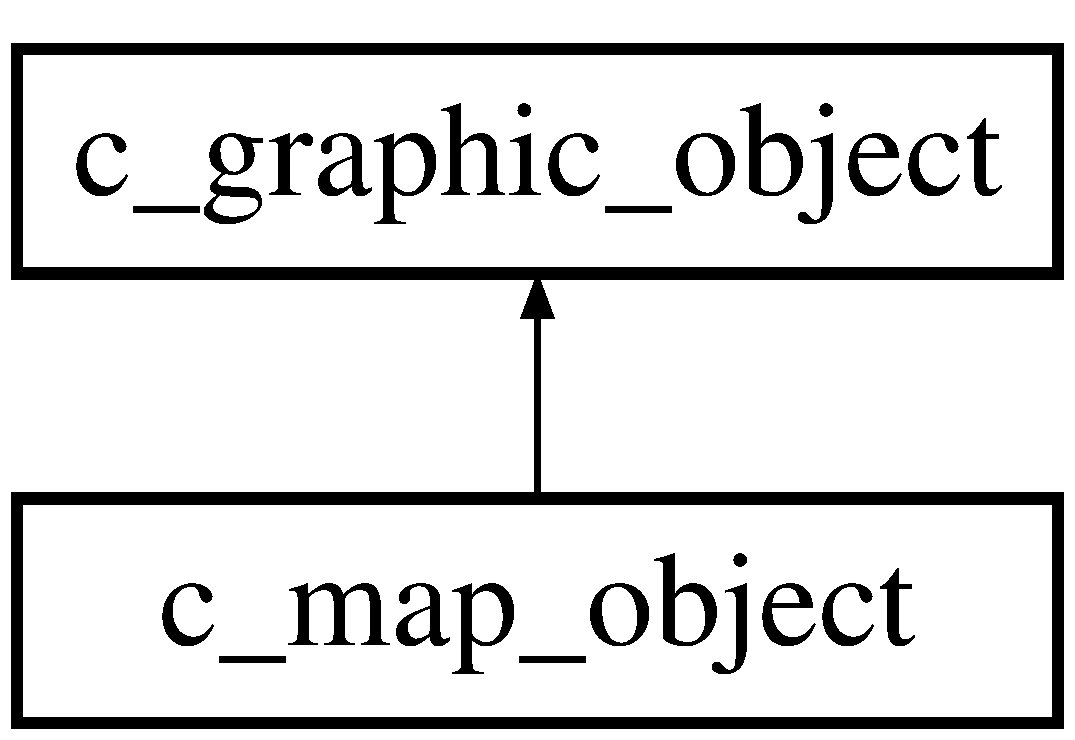
\includegraphics[height=2.000000cm]{classc__map__object}
\end{center}
\end{figure}
\subsection*{Public Member Functions}
\begin{DoxyCompactItemize}
\item 
\hyperlink{classc__map__object_af35bc3b68a2c2f756b67cc1a5b73dde3}{c\-\_\-map\-\_\-object} (t\-\_\-object\-\_\-type object\-\_\-type, int \hyperlink{classc__map__object_a4563fd9421b83b1349e4e74559b22507}{link\-\_\-id}, int \hyperlink{classc__map__object_a95575848075ef4b407907eb8e5c48e3c}{link\-\_\-id2}, long int $\ast$\hyperlink{classc__graphic__object_a9ff91aa7a60272a8f713ff011a0cc0bb}{global\-\_\-time})
\item 
\hyperlink{classc__map__object_a92cf99f145db3d9b56b94571c929564d}{$\sim$c\-\_\-map\-\_\-object} ()
\item 
void \hyperlink{classc__map__object_a1ac16227e406d56484c55089ecbffd48}{update\-\_\-controlled\-\_\-objects} ()
\item 
void \hyperlink{classc__map__object_a422769b2c8cb02575457f10113ef369c}{add\-\_\-controlled\-\_\-objects} (int number\-\_\-of\-\_\-objects, \hyperlink{classc__map__object}{c\-\_\-map\-\_\-object} $\ast$objects\mbox{[}$\,$\mbox{]})
\item 
t\-\_\-object\-\_\-type \hyperlink{classc__map__object_a29b6c2ae995c04000f76dc1e9776e3a2}{get\-\_\-type} ()
\item 
int \hyperlink{classc__map__object_afb6cfb99e3c9387c2470d94f8370ec28}{get\-\_\-link\-\_\-id} ()
\item 
int \hyperlink{classc__map__object_a138d547da618a4a3ce5e10cdb35989fd}{get\-\_\-link\-\_\-id2} ()
\item 
t\-\_\-object\-\_\-state \hyperlink{classc__map__object_a7e78aa3675f4053ec9f35730a4a8d9a4}{get\-\_\-state} ()
\item 
bool \hyperlink{classc__map__object_ab79a3d3c7a6e4a7170d8ddb7b648c782}{is\-\_\-input} ()
\item 
void \hyperlink{classc__map__object_ae16327caf95e5c4eaae2abc09a57b272}{set\-\_\-state} (t\-\_\-object\-\_\-state \hyperlink{classc__map__object_a8bde4cfd4fed11a9f01389977504a10a}{object\-\_\-state})
\item 
void \hyperlink{classc__map__object_acf08ee03ad8b6751611800aa57b190bd}{switch\-\_\-state} ()
\item 
virtual void \hyperlink{classc__map__object_add8a45bcf4f77ba65716095c05483f4f}{draw} (int x, int y)
\item 
bool \hyperlink{classc__map__object_ad234b9747a048875128fba677136ef4f}{is\-\_\-stepable} ()
\item 
void \hyperlink{classc__map__object_a38d45962c3bbc6ae6f2572811be93214}{use} ()
\item 
void \hyperlink{classc__map__object_a2df801781fdad9a4b42a78ff5b9c8558}{update\-\_\-animation\-\_\-period} ()
\item 
bool \hyperlink{classc__map__object_aad8f98a195de734d0cfa94c93fc94406}{compare\-\_\-link\-\_\-ids} (\hyperlink{classc__map__object}{c\-\_\-map\-\_\-object} $\ast$another\-\_\-object)
\item 
\hyperlink{classc__map__object}{c\-\_\-map\-\_\-object} $\ast$ \hyperlink{classc__map__object_a63cc574e5972757e2a399a6ddc63efc3}{get\-\_\-controlled\-\_\-object} (int index)
\item 
void \hyperlink{classc__map__object_a577ec7d3dd41b29e6c5f554d6c3d600f}{set\-\_\-sign\-\_\-text} (string text)
\item 
string \hyperlink{classc__map__object_ad5c4284b4e7b5a824ae5734f33f59f35}{get\-\_\-sign\-\_\-text} ()
\end{DoxyCompactItemize}
\subsection*{Protected Attributes}
\begin{DoxyCompactItemize}
\item 
t\-\_\-object\-\_\-type \hyperlink{classc__map__object_a9d47ec81d25e5785311adc675ea6377d}{type}
\item 
int \hyperlink{classc__map__object_a4563fd9421b83b1349e4e74559b22507}{link\-\_\-id}
\item 
int \hyperlink{classc__map__object_a95575848075ef4b407907eb8e5c48e3c}{link\-\_\-id2}
\item 
bool \hyperlink{classc__map__object_a67285c4371f63f7a3e31e81d89696271}{input}
\item 
t\-\_\-object\-\_\-state \hyperlink{classc__map__object_a8bde4cfd4fed11a9f01389977504a10a}{object\-\_\-state}
\item 
A\-L\-L\-E\-G\-R\-O\-\_\-\-B\-I\-T\-M\-A\-P $\ast$ \hyperlink{classc__map__object_af9e944bd38ae90bfa3f9f051ec9dd8fa}{bitmaps} \mbox{[}5\mbox{]}
\item 
bool \hyperlink{classc__map__object_a89b2a794cb8409e93493a99adfe2d311}{stepable}
\item 
\hyperlink{classc__map__object}{c\-\_\-map\-\_\-object} $\ast$$\ast$ \hyperlink{classc__map__object_af772ed08fc85de963e5cd18b403eecca}{controlling}
\item 
int \hyperlink{classc__map__object_ad03a55702a3f84a90bfa46700ab7124c}{number\-\_\-of\-\_\-controlled}
\item 
string \hyperlink{classc__map__object_a57a973ea5b89a30e3b9f9b1332197493}{sign\-\_\-text}
\end{DoxyCompactItemize}


\subsection{Detailed Description}
Map object class header file.

authors\-: Miloslav Číž year\-: 2013 

\subsection{Constructor \& Destructor Documentation}
\hypertarget{classc__map__object_af35bc3b68a2c2f756b67cc1a5b73dde3}{\index{c\-\_\-map\-\_\-object@{c\-\_\-map\-\_\-object}!c\-\_\-map\-\_\-object@{c\-\_\-map\-\_\-object}}
\index{c\-\_\-map\-\_\-object@{c\-\_\-map\-\_\-object}!c_map_object@{c\-\_\-map\-\_\-object}}
\subsubsection[{c\-\_\-map\-\_\-object}]{\setlength{\rightskip}{0pt plus 5cm}c\-\_\-map\-\_\-object\-::c\-\_\-map\-\_\-object (
\begin{DoxyParamCaption}
\item[{t\-\_\-object\-\_\-type}]{object\-\_\-type, }
\item[{int}]{link\-\_\-id, }
\item[{int}]{link\-\_\-id2, }
\item[{long int $\ast$}]{global\-\_\-time}
\end{DoxyParamCaption}
)}}\label{classc__map__object_af35bc3b68a2c2f756b67cc1a5b73dde3}
text -\/ only for sign objects

Map object class implementation file.

authors\-: Miloslav Číž year\-: 2013 \hypertarget{classc__map__object_a92cf99f145db3d9b56b94571c929564d}{\index{c\-\_\-map\-\_\-object@{c\-\_\-map\-\_\-object}!$\sim$c\-\_\-map\-\_\-object@{$\sim$c\-\_\-map\-\_\-object}}
\index{$\sim$c\-\_\-map\-\_\-object@{$\sim$c\-\_\-map\-\_\-object}!c_map_object@{c\-\_\-map\-\_\-object}}
\subsubsection[{$\sim$c\-\_\-map\-\_\-object}]{\setlength{\rightskip}{0pt plus 5cm}c\-\_\-map\-\_\-object\-::$\sim$c\-\_\-map\-\_\-object (
\begin{DoxyParamCaption}
{}
\end{DoxyParamCaption}
)}}\label{classc__map__object_a92cf99f145db3d9b56b94571c929564d}
Class constructor, initialises new map object.


\begin{DoxyParams}{Parameters}
{\em object\-\_\-type} & object type of the new map object. \\
\hline
{\em link\-\_\-id} & a number identifying the connection between objects, objects with same link id will affect each other \\
\hline
{\em link\-\_\-id2} & another link id, negative number means this will not be used \\
\hline
{\em global\-\_\-time} & reference to a global time counter variable which is needed for animations \\
\hline
\end{DoxyParams}


\subsection{Member Function Documentation}
\hypertarget{classc__map__object_a422769b2c8cb02575457f10113ef369c}{\index{c\-\_\-map\-\_\-object@{c\-\_\-map\-\_\-object}!add\-\_\-controlled\-\_\-objects@{add\-\_\-controlled\-\_\-objects}}
\index{add\-\_\-controlled\-\_\-objects@{add\-\_\-controlled\-\_\-objects}!c_map_object@{c\-\_\-map\-\_\-object}}
\subsubsection[{add\-\_\-controlled\-\_\-objects}]{\setlength{\rightskip}{0pt plus 5cm}void c\-\_\-map\-\_\-object\-::add\-\_\-controlled\-\_\-objects (
\begin{DoxyParamCaption}
\item[{int}]{number\-\_\-of\-\_\-objects, }
\item[{{\bf c\-\_\-map\-\_\-object} $\ast$}]{objects\mbox{[}$\,$\mbox{]}}
\end{DoxyParamCaption}
)}}\label{classc__map__object_a422769b2c8cb02575457f10113ef369c}
Updated states of objects that are controlled by this object. \hypertarget{classc__map__object_aad8f98a195de734d0cfa94c93fc94406}{\index{c\-\_\-map\-\_\-object@{c\-\_\-map\-\_\-object}!compare\-\_\-link\-\_\-ids@{compare\-\_\-link\-\_\-ids}}
\index{compare\-\_\-link\-\_\-ids@{compare\-\_\-link\-\_\-ids}!c_map_object@{c\-\_\-map\-\_\-object}}
\subsubsection[{compare\-\_\-link\-\_\-ids}]{\setlength{\rightskip}{0pt plus 5cm}bool c\-\_\-map\-\_\-object\-::compare\-\_\-link\-\_\-ids (
\begin{DoxyParamCaption}
\item[{{\bf c\-\_\-map\-\_\-object} $\ast$}]{another\-\_\-object}
\end{DoxyParamCaption}
)}}\label{classc__map__object_aad8f98a195de734d0cfa94c93fc94406}
Depending on current animation sets the animation period attribute. \hypertarget{classc__map__object_add8a45bcf4f77ba65716095c05483f4f}{\index{c\-\_\-map\-\_\-object@{c\-\_\-map\-\_\-object}!draw@{draw}}
\index{draw@{draw}!c_map_object@{c\-\_\-map\-\_\-object}}
\subsubsection[{draw}]{\setlength{\rightskip}{0pt plus 5cm}void c\-\_\-map\-\_\-object\-::draw (
\begin{DoxyParamCaption}
\item[{int}]{x, }
\item[{int}]{y}
\end{DoxyParamCaption}
)\hspace{0.3cm}{\ttfamily [virtual]}}}\label{classc__map__object_add8a45bcf4f77ba65716095c05483f4f}
Switches states of the object between on and off. 

Reimplemented from \hyperlink{classc__graphic__object_a94ef8137eed9ce1ae7adf366fefb51cf}{c\-\_\-graphic\-\_\-object}.

\hypertarget{classc__map__object_a63cc574e5972757e2a399a6ddc63efc3}{\index{c\-\_\-map\-\_\-object@{c\-\_\-map\-\_\-object}!get\-\_\-controlled\-\_\-object@{get\-\_\-controlled\-\_\-object}}
\index{get\-\_\-controlled\-\_\-object@{get\-\_\-controlled\-\_\-object}!c_map_object@{c\-\_\-map\-\_\-object}}
\subsubsection[{get\-\_\-controlled\-\_\-object}]{\setlength{\rightskip}{0pt plus 5cm}{\bf c\-\_\-map\-\_\-object} $\ast$ c\-\_\-map\-\_\-object\-::get\-\_\-controlled\-\_\-object (
\begin{DoxyParamCaption}
\item[{int}]{index}
\end{DoxyParamCaption}
)}}\label{classc__map__object_a63cc574e5972757e2a399a6ddc63efc3}
Checks if this map object and another map object are linked via their link ids.


\begin{DoxyParams}{Parameters}
{\em another\-\_\-object} & object to be compared to this object by link ids \\
\hline
\end{DoxyParams}
\begin{DoxyReturn}{Returns}
true if this object is linked with another\-\_\-object, otherwise false 
\end{DoxyReturn}
\hypertarget{classc__map__object_afb6cfb99e3c9387c2470d94f8370ec28}{\index{c\-\_\-map\-\_\-object@{c\-\_\-map\-\_\-object}!get\-\_\-link\-\_\-id@{get\-\_\-link\-\_\-id}}
\index{get\-\_\-link\-\_\-id@{get\-\_\-link\-\_\-id}!c_map_object@{c\-\_\-map\-\_\-object}}
\subsubsection[{get\-\_\-link\-\_\-id}]{\setlength{\rightskip}{0pt plus 5cm}int c\-\_\-map\-\_\-object\-::get\-\_\-link\-\_\-id (
\begin{DoxyParamCaption}
{}
\end{DoxyParamCaption}
)}}\label{classc__map__object_afb6cfb99e3c9387c2470d94f8370ec28}
Returns this object's type.

\begin{DoxyReturn}{Returns}
this object's type 
\end{DoxyReturn}
\hypertarget{classc__map__object_a138d547da618a4a3ce5e10cdb35989fd}{\index{c\-\_\-map\-\_\-object@{c\-\_\-map\-\_\-object}!get\-\_\-link\-\_\-id2@{get\-\_\-link\-\_\-id2}}
\index{get\-\_\-link\-\_\-id2@{get\-\_\-link\-\_\-id2}!c_map_object@{c\-\_\-map\-\_\-object}}
\subsubsection[{get\-\_\-link\-\_\-id2}]{\setlength{\rightskip}{0pt plus 5cm}int c\-\_\-map\-\_\-object\-::get\-\_\-link\-\_\-id2 (
\begin{DoxyParamCaption}
{}
\end{DoxyParamCaption}
)}}\label{classc__map__object_a138d547da618a4a3ce5e10cdb35989fd}
Returns the object's link id.

\begin{DoxyReturn}{Returns}
object link id 
\end{DoxyReturn}
\hypertarget{classc__map__object_ad5c4284b4e7b5a824ae5734f33f59f35}{\index{c\-\_\-map\-\_\-object@{c\-\_\-map\-\_\-object}!get\-\_\-sign\-\_\-text@{get\-\_\-sign\-\_\-text}}
\index{get\-\_\-sign\-\_\-text@{get\-\_\-sign\-\_\-text}!c_map_object@{c\-\_\-map\-\_\-object}}
\subsubsection[{get\-\_\-sign\-\_\-text}]{\setlength{\rightskip}{0pt plus 5cm}string c\-\_\-map\-\_\-object\-::get\-\_\-sign\-\_\-text (
\begin{DoxyParamCaption}
{}
\end{DoxyParamCaption}
)}}\label{classc__map__object_ad5c4284b4e7b5a824ae5734f33f59f35}
Sets the text for sign map object.


\begin{DoxyParams}{Parameters}
{\em text} & text to be set \\
\hline
\end{DoxyParams}
\hypertarget{classc__map__object_a7e78aa3675f4053ec9f35730a4a8d9a4}{\index{c\-\_\-map\-\_\-object@{c\-\_\-map\-\_\-object}!get\-\_\-state@{get\-\_\-state}}
\index{get\-\_\-state@{get\-\_\-state}!c_map_object@{c\-\_\-map\-\_\-object}}
\subsubsection[{get\-\_\-state}]{\setlength{\rightskip}{0pt plus 5cm}t\-\_\-object\-\_\-state c\-\_\-map\-\_\-object\-::get\-\_\-state (
\begin{DoxyParamCaption}
{}
\end{DoxyParamCaption}
)}}\label{classc__map__object_a7e78aa3675f4053ec9f35730a4a8d9a4}
Returns the object's secondary link id.

\begin{DoxyReturn}{Returns}
object secondary link id 
\end{DoxyReturn}
\hypertarget{classc__map__object_a29b6c2ae995c04000f76dc1e9776e3a2}{\index{c\-\_\-map\-\_\-object@{c\-\_\-map\-\_\-object}!get\-\_\-type@{get\-\_\-type}}
\index{get\-\_\-type@{get\-\_\-type}!c_map_object@{c\-\_\-map\-\_\-object}}
\subsubsection[{get\-\_\-type}]{\setlength{\rightskip}{0pt plus 5cm}t\-\_\-object\-\_\-type c\-\_\-map\-\_\-object\-::get\-\_\-type (
\begin{DoxyParamCaption}
{}
\end{DoxyParamCaption}
)}}\label{classc__map__object_a29b6c2ae995c04000f76dc1e9776e3a2}
Registers objects that will be controlled by this object.


\begin{DoxyParams}{Parameters}
{\em number\-\_\-of\-\_\-objects} & length of objects array \\
\hline
{\em objects} & array of pointers to objects that will be controlled \\
\hline
\end{DoxyParams}
\hypertarget{classc__map__object_ab79a3d3c7a6e4a7170d8ddb7b648c782}{\index{c\-\_\-map\-\_\-object@{c\-\_\-map\-\_\-object}!is\-\_\-input@{is\-\_\-input}}
\index{is\-\_\-input@{is\-\_\-input}!c_map_object@{c\-\_\-map\-\_\-object}}
\subsubsection[{is\-\_\-input}]{\setlength{\rightskip}{0pt plus 5cm}bool c\-\_\-map\-\_\-object\-::is\-\_\-input (
\begin{DoxyParamCaption}
{}
\end{DoxyParamCaption}
)}}\label{classc__map__object_ab79a3d3c7a6e4a7170d8ddb7b648c782}
Returns the object's state.

\begin{DoxyReturn}{Returns}
object state 
\end{DoxyReturn}
\hypertarget{classc__map__object_ad234b9747a048875128fba677136ef4f}{\index{c\-\_\-map\-\_\-object@{c\-\_\-map\-\_\-object}!is\-\_\-stepable@{is\-\_\-stepable}}
\index{is\-\_\-stepable@{is\-\_\-stepable}!c_map_object@{c\-\_\-map\-\_\-object}}
\subsubsection[{is\-\_\-stepable}]{\setlength{\rightskip}{0pt plus 5cm}bool c\-\_\-map\-\_\-object\-::is\-\_\-stepable (
\begin{DoxyParamCaption}
{}
\end{DoxyParamCaption}
)}}\label{classc__map__object_ad234b9747a048875128fba677136ef4f}
Draws the map at given position on the screen.


\begin{DoxyParams}{Parameters}
{\em x} & x position of the screen \\
\hline
{\em y} & y position of the screen \\
\hline
\end{DoxyParams}
\hypertarget{classc__map__object_a577ec7d3dd41b29e6c5f554d6c3d600f}{\index{c\-\_\-map\-\_\-object@{c\-\_\-map\-\_\-object}!set\-\_\-sign\-\_\-text@{set\-\_\-sign\-\_\-text}}
\index{set\-\_\-sign\-\_\-text@{set\-\_\-sign\-\_\-text}!c_map_object@{c\-\_\-map\-\_\-object}}
\subsubsection[{set\-\_\-sign\-\_\-text}]{\setlength{\rightskip}{0pt plus 5cm}void c\-\_\-map\-\_\-object\-::set\-\_\-sign\-\_\-text (
\begin{DoxyParamCaption}
\item[{string}]{text}
\end{DoxyParamCaption}
)}}\label{classc__map__object_a577ec7d3dd41b29e6c5f554d6c3d600f}
Returns one of objects controlled by this object.


\begin{DoxyParams}{Parameters}
{\em index} & index of the controlled objects to be returned \\
\hline
\end{DoxyParams}
\begin{DoxyReturn}{Returns}
pointer to controlled object at given index, if the index exceeds length of object list, N\-U\-L\-L is returned 
\end{DoxyReturn}
\hypertarget{classc__map__object_ae16327caf95e5c4eaae2abc09a57b272}{\index{c\-\_\-map\-\_\-object@{c\-\_\-map\-\_\-object}!set\-\_\-state@{set\-\_\-state}}
\index{set\-\_\-state@{set\-\_\-state}!c_map_object@{c\-\_\-map\-\_\-object}}
\subsubsection[{set\-\_\-state}]{\setlength{\rightskip}{0pt plus 5cm}void c\-\_\-map\-\_\-object\-::set\-\_\-state (
\begin{DoxyParamCaption}
\item[{t\-\_\-object\-\_\-state}]{object\-\_\-state}
\end{DoxyParamCaption}
)}}\label{classc__map__object_ae16327caf95e5c4eaae2abc09a57b272}
Checks if this object is an input object.

\begin{DoxyReturn}{Returns}
true, if this object is input, otherwise false 
\end{DoxyReturn}
\hypertarget{classc__map__object_acf08ee03ad8b6751611800aa57b190bd}{\index{c\-\_\-map\-\_\-object@{c\-\_\-map\-\_\-object}!switch\-\_\-state@{switch\-\_\-state}}
\index{switch\-\_\-state@{switch\-\_\-state}!c_map_object@{c\-\_\-map\-\_\-object}}
\subsubsection[{switch\-\_\-state}]{\setlength{\rightskip}{0pt plus 5cm}void c\-\_\-map\-\_\-object\-::switch\-\_\-state (
\begin{DoxyParamCaption}
{}
\end{DoxyParamCaption}
)}}\label{classc__map__object_acf08ee03ad8b6751611800aa57b190bd}
Sets the object's state (but does nothing else like updating controlled objects etc.).


\begin{DoxyParams}{Parameters}
{\em object\-\_\-state} & new object state \\
\hline
\end{DoxyParams}
\hypertarget{classc__map__object_a2df801781fdad9a4b42a78ff5b9c8558}{\index{c\-\_\-map\-\_\-object@{c\-\_\-map\-\_\-object}!update\-\_\-animation\-\_\-period@{update\-\_\-animation\-\_\-period}}
\index{update\-\_\-animation\-\_\-period@{update\-\_\-animation\-\_\-period}!c_map_object@{c\-\_\-map\-\_\-object}}
\subsubsection[{update\-\_\-animation\-\_\-period}]{\setlength{\rightskip}{0pt plus 5cm}void c\-\_\-map\-\_\-object\-::update\-\_\-animation\-\_\-period (
\begin{DoxyParamCaption}
{}
\end{DoxyParamCaption}
)\hspace{0.3cm}{\ttfamily [virtual]}}}\label{classc__map__object_a2df801781fdad9a4b42a78ff5b9c8558}
This method is called when player uses the object. 

Reimplemented from \hyperlink{classc__graphic__object_a20fa3f61532b73f64f3307fd14b7dba6}{c\-\_\-graphic\-\_\-object}.

\hypertarget{classc__map__object_a1ac16227e406d56484c55089ecbffd48}{\index{c\-\_\-map\-\_\-object@{c\-\_\-map\-\_\-object}!update\-\_\-controlled\-\_\-objects@{update\-\_\-controlled\-\_\-objects}}
\index{update\-\_\-controlled\-\_\-objects@{update\-\_\-controlled\-\_\-objects}!c_map_object@{c\-\_\-map\-\_\-object}}
\subsubsection[{update\-\_\-controlled\-\_\-objects}]{\setlength{\rightskip}{0pt plus 5cm}void c\-\_\-map\-\_\-object\-::update\-\_\-controlled\-\_\-objects (
\begin{DoxyParamCaption}
{}
\end{DoxyParamCaption}
)}}\label{classc__map__object_a1ac16227e406d56484c55089ecbffd48}
Class destructor, frees all its memory. \hypertarget{classc__map__object_a38d45962c3bbc6ae6f2572811be93214}{\index{c\-\_\-map\-\_\-object@{c\-\_\-map\-\_\-object}!use@{use}}
\index{use@{use}!c_map_object@{c\-\_\-map\-\_\-object}}
\subsubsection[{use}]{\setlength{\rightskip}{0pt plus 5cm}void c\-\_\-map\-\_\-object\-::use (
\begin{DoxyParamCaption}
{}
\end{DoxyParamCaption}
)}}\label{classc__map__object_a38d45962c3bbc6ae6f2572811be93214}
Checks whether this object can be stepped over.

\begin{DoxyReturn}{Returns}
true if this object is stepable, otherwise false 
\end{DoxyReturn}


\subsection{Member Data Documentation}
\hypertarget{classc__map__object_af9e944bd38ae90bfa3f9f051ec9dd8fa}{\index{c\-\_\-map\-\_\-object@{c\-\_\-map\-\_\-object}!bitmaps@{bitmaps}}
\index{bitmaps@{bitmaps}!c_map_object@{c\-\_\-map\-\_\-object}}
\subsubsection[{bitmaps}]{\setlength{\rightskip}{0pt plus 5cm}A\-L\-L\-E\-G\-R\-O\-\_\-\-B\-I\-T\-M\-A\-P$\ast$ c\-\_\-map\-\_\-object\-::bitmaps\mbox{[}5\mbox{]}\hspace{0.3cm}{\ttfamily [protected]}}}\label{classc__map__object_af9e944bd38ae90bfa3f9f051ec9dd8fa}
identifies object state (on/off, open/closed etc.) \hypertarget{classc__map__object_af772ed08fc85de963e5cd18b403eecca}{\index{c\-\_\-map\-\_\-object@{c\-\_\-map\-\_\-object}!controlling@{controlling}}
\index{controlling@{controlling}!c_map_object@{c\-\_\-map\-\_\-object}}
\subsubsection[{controlling}]{\setlength{\rightskip}{0pt plus 5cm}{\bf c\-\_\-map\-\_\-object}$\ast$$\ast$ c\-\_\-map\-\_\-object\-::controlling\hspace{0.3cm}{\ttfamily [protected]}}}\label{classc__map__object_af772ed08fc85de963e5cd18b403eecca}
true if this object can be stepped over \hypertarget{classc__map__object_a67285c4371f63f7a3e31e81d89696271}{\index{c\-\_\-map\-\_\-object@{c\-\_\-map\-\_\-object}!input@{input}}
\index{input@{input}!c_map_object@{c\-\_\-map\-\_\-object}}
\subsubsection[{input}]{\setlength{\rightskip}{0pt plus 5cm}bool c\-\_\-map\-\_\-object\-::input\hspace{0.3cm}{\ttfamily [protected]}}}\label{classc__map__object_a67285c4371f63f7a3e31e81d89696271}
another link, negative number means it's not used \hypertarget{classc__map__object_a4563fd9421b83b1349e4e74559b22507}{\index{c\-\_\-map\-\_\-object@{c\-\_\-map\-\_\-object}!link\-\_\-id@{link\-\_\-id}}
\index{link\-\_\-id@{link\-\_\-id}!c_map_object@{c\-\_\-map\-\_\-object}}
\subsubsection[{link\-\_\-id}]{\setlength{\rightskip}{0pt plus 5cm}int c\-\_\-map\-\_\-object\-::link\-\_\-id\hspace{0.3cm}{\ttfamily [protected]}}}\label{classc__map__object_a4563fd9421b83b1349e4e74559b22507}
type of the object \hypertarget{classc__map__object_a95575848075ef4b407907eb8e5c48e3c}{\index{c\-\_\-map\-\_\-object@{c\-\_\-map\-\_\-object}!link\-\_\-id2@{link\-\_\-id2}}
\index{link\-\_\-id2@{link\-\_\-id2}!c_map_object@{c\-\_\-map\-\_\-object}}
\subsubsection[{link\-\_\-id2}]{\setlength{\rightskip}{0pt plus 5cm}int c\-\_\-map\-\_\-object\-::link\-\_\-id2\hspace{0.3cm}{\ttfamily [protected]}}}\label{classc__map__object_a95575848075ef4b407907eb8e5c48e3c}
identifies link between objects so they affect each other \hypertarget{classc__map__object_ad03a55702a3f84a90bfa46700ab7124c}{\index{c\-\_\-map\-\_\-object@{c\-\_\-map\-\_\-object}!number\-\_\-of\-\_\-controlled@{number\-\_\-of\-\_\-controlled}}
\index{number\-\_\-of\-\_\-controlled@{number\-\_\-of\-\_\-controlled}!c_map_object@{c\-\_\-map\-\_\-object}}
\subsubsection[{number\-\_\-of\-\_\-controlled}]{\setlength{\rightskip}{0pt plus 5cm}int c\-\_\-map\-\_\-object\-::number\-\_\-of\-\_\-controlled\hspace{0.3cm}{\ttfamily [protected]}}}\label{classc__map__object_ad03a55702a3f84a90bfa46700ab7124c}
array of pointers to objects which are affected by this object \hypertarget{classc__map__object_a8bde4cfd4fed11a9f01389977504a10a}{\index{c\-\_\-map\-\_\-object@{c\-\_\-map\-\_\-object}!object\-\_\-state@{object\-\_\-state}}
\index{object\-\_\-state@{object\-\_\-state}!c_map_object@{c\-\_\-map\-\_\-object}}
\subsubsection[{object\-\_\-state}]{\setlength{\rightskip}{0pt plus 5cm}t\-\_\-object\-\_\-state c\-\_\-map\-\_\-object\-::object\-\_\-state\hspace{0.3cm}{\ttfamily [protected]}}}\label{classc__map__object_a8bde4cfd4fed11a9f01389977504a10a}
true if this object is input (ie. lever, button, etc.) \hypertarget{classc__map__object_a57a973ea5b89a30e3b9f9b1332197493}{\index{c\-\_\-map\-\_\-object@{c\-\_\-map\-\_\-object}!sign\-\_\-text@{sign\-\_\-text}}
\index{sign\-\_\-text@{sign\-\_\-text}!c_map_object@{c\-\_\-map\-\_\-object}}
\subsubsection[{sign\-\_\-text}]{\setlength{\rightskip}{0pt plus 5cm}string c\-\_\-map\-\_\-object\-::sign\-\_\-text\hspace{0.3cm}{\ttfamily [protected]}}}\label{classc__map__object_a57a973ea5b89a30e3b9f9b1332197493}
length of controlled array \hypertarget{classc__map__object_a89b2a794cb8409e93493a99adfe2d311}{\index{c\-\_\-map\-\_\-object@{c\-\_\-map\-\_\-object}!stepable@{stepable}}
\index{stepable@{stepable}!c_map_object@{c\-\_\-map\-\_\-object}}
\subsubsection[{stepable}]{\setlength{\rightskip}{0pt plus 5cm}bool c\-\_\-map\-\_\-object\-::stepable\hspace{0.3cm}{\ttfamily [protected]}}}\label{classc__map__object_a89b2a794cb8409e93493a99adfe2d311}
bitmaps used to draw this object \hypertarget{classc__map__object_a9d47ec81d25e5785311adc675ea6377d}{\index{c\-\_\-map\-\_\-object@{c\-\_\-map\-\_\-object}!type@{type}}
\index{type@{type}!c_map_object@{c\-\_\-map\-\_\-object}}
\subsubsection[{type}]{\setlength{\rightskip}{0pt plus 5cm}t\-\_\-object\-\_\-type c\-\_\-map\-\_\-object\-::type\hspace{0.3cm}{\ttfamily [protected]}}}\label{classc__map__object_a9d47ec81d25e5785311adc675ea6377d}
This class is a map object, such as a tree or a lever. 

The documentation for this class was generated from the following files\-:\begin{DoxyCompactItemize}
\item 
magerage/map\-\_\-object.\-h\item 
magerage/map\-\_\-object.\-cpp\end{DoxyCompactItemize}

\hypertarget{classc__menu}{\section{c\-\_\-menu Class Reference}
\label{classc__menu}\index{c\-\_\-menu@{c\-\_\-menu}}
}
\subsection*{Public Member Functions}
\begin{DoxyCompactItemize}
\item 
\hyperlink{classc__menu_a56fe0346fcf0fcc7c351f52cfcf5adea}{c\-\_\-menu} (\hyperlink{structt__input__output__state}{t\-\_\-input\-\_\-output\-\_\-state} $\ast$input\-\_\-output\-\_\-state)
\item 
\hyperlink{classc__menu_ac8a06810d4e60f8cb2f74a82f8863759}{$\sim$c\-\_\-menu} ()
\item 
void \hyperlink{classc__menu_a35b817db8d2fa0d78dee6696846524c2}{set\-\_\-menu\-\_\-items} (string items\mbox{[}$\,$\mbox{]}, int number\-\_\-of\-\_\-items, string \hyperlink{classc__menu_a04174390379e68ec20a0ec5945748570}{title}, bool keep\-\_\-cursor)
\item 
void \hyperlink{classc__menu_afcaeabf86dfb9d715548bd8277d4bce8}{display\-\_\-easter\-\_\-egg} ()
\item 
void \hyperlink{classc__menu_ae609e23056e45e3da00fbd763d31c6fe}{set\-\_\-menu\-\_\-info\-\_\-screen} (string image\-\_\-path, string \hyperlink{classc__menu_ade57856309857147f055d82f1e7d839e}{text\-\_\-lines}\mbox{[}$\,$\mbox{]}, int number\-\_\-of\-\_\-lines, double duration, unsigned char bg\-\_\-red, unsigned char bg\-\_\-green, unsigned char bg\-\_\-blue)
\item 
void \hyperlink{classc__menu_afe00a1ae7c5f70012e3e4c510cbb2bbe}{set\-\_\-menu\-\_\-choose\-\_\-level} (int \hyperlink{classc__menu_a3fe87a5b76e64557af759a180b0bb0ae}{number\-\_\-of\-\_\-levels})
\item 
int \hyperlink{classc__menu_a13affcab2aced75886f74ff70d17b509}{update} ()
\end{DoxyCompactItemize}
\subsection*{Protected Attributes}
\begin{DoxyCompactItemize}
\item 
t\-\_\-menu\-\_\-type \hyperlink{classc__menu_a1e0be6c7749c393b11b4a1f8330588f8}{menu\-\_\-type}
\item 
int \hyperlink{classc__menu_a5ccfb7e7c08dd3b70b7ddf5fd1f00308}{current\-\_\-item}
\item 
int \hyperlink{classc__menu_a4000a7ae156999a6e2ea273ab328a0f1}{number\-\_\-of\-\_\-text\-\_\-lines}
\item 
string \hyperlink{classc__menu_ade57856309857147f055d82f1e7d839e}{text\-\_\-lines} \mbox{[}10\mbox{]}
\item 
int \hyperlink{classc__menu_a3fe87a5b76e64557af759a180b0bb0ae}{number\-\_\-of\-\_\-levels}
\item 
\hyperlink{structt__input__output__state}{t\-\_\-input\-\_\-output\-\_\-state} $\ast$ \hyperlink{classc__menu_ae21342c5213a9d1f75932af186f65327}{io}
\item 
boolean \hyperlink{classc__menu_a3181439816433cf8a2b42dcaf7fbfea7}{pressed}
\item 
double \hyperlink{classc__menu_ae035b1a97b2334a285e3db7e00b0bdac}{effect\-\_\-time}
\item 
double \hyperlink{classc__menu_a55a8c30640f0cd40b1ac7db29644d050}{screen\-\_\-end\-\_\-time}
\item 
bool \hyperlink{classc__menu_ae983a894c3afee8671ed9f0fefd1b6a9}{fading\-\_\-in}
\item 
bool \hyperlink{classc__menu_a72afb1bd10e583b642922b2a3b1d799b}{fading\-\_\-out}
\item 
string \hyperlink{classc__menu_a04174390379e68ec20a0ec5945748570}{title}
\item 
unsigned char \hyperlink{classc__menu_a24f640c1886fdf22053a50f8700d559f}{bg\-\_\-color} \mbox{[}3\mbox{]}
\item 
double \hyperlink{classc__menu_af9c750db5db9b548d4d936e30dfe314f}{easter\-\_\-egg\-\_\-started}
\item 
int \hyperlink{classc__menu_a39f79196e63fb1e14ac437c2d88c8c7d}{level\-\_\-number\-\_\-positions\-\_\-x} \mbox{[}22\mbox{]}
\item 
int \hyperlink{classc__menu_ac4f208edba8bee1d6184db03e3a89e41}{level\-\_\-number\-\_\-positions\-\_\-y} \mbox{[}22\mbox{]}
\item 
A\-L\-L\-E\-G\-R\-O\-\_\-\-B\-I\-T\-M\-A\-P $\ast$ \hyperlink{classc__menu_a0f70bbd0314bd3da93df8ab3f1df3a70}{menu\-\_\-top}
\item 
A\-L\-L\-E\-G\-R\-O\-\_\-\-B\-I\-T\-M\-A\-P $\ast$ \hyperlink{classc__menu_a2c6c75c1a53e6f375cadbda437cb99f5}{menu\-\_\-middle}
\item 
A\-L\-L\-E\-G\-R\-O\-\_\-\-B\-I\-T\-M\-A\-P $\ast$ \hyperlink{classc__menu_a74ca4baf7d4dbe8c0b6a4d2e52142ba4}{menu\-\_\-bottom}
\item 
A\-L\-L\-E\-G\-R\-O\-\_\-\-B\-I\-T\-M\-A\-P $\ast$ \hyperlink{classc__menu_a7704ebdcc1c29c16e0b400ce9be6b933}{menu\-\_\-selection}
\item 
A\-L\-L\-E\-G\-R\-O\-\_\-\-B\-I\-T\-M\-A\-P $\ast$ \hyperlink{classc__menu_a2898c943cc19bc36d9cb3763b9dc3c03}{info\-\_\-background}
\item 
A\-L\-L\-E\-G\-R\-O\-\_\-\-B\-I\-T\-M\-A\-P $\ast$ \hyperlink{classc__menu_af61b3585bbce811355a9522f4d4e5ee1}{menu\-\_\-border}
\item 
A\-L\-L\-E\-G\-R\-O\-\_\-\-B\-I\-T\-M\-A\-P $\ast$ \hyperlink{classc__menu_a823fbb421af347ddd1c891fec53c242d}{easter\-\_\-egg}
\item 
A\-L\-L\-E\-G\-R\-O\-\_\-\-F\-O\-N\-T $\ast$ \hyperlink{classc__menu_a51aa6761c97638a2d3d3e34213a0fc25}{text\-\_\-font}
\item 
A\-L\-L\-E\-G\-R\-O\-\_\-\-S\-A\-M\-P\-L\-E $\ast$ \hyperlink{classc__menu_a697e104d6bb5ac42a46a0a8076a82444}{click\-\_\-sound}
\end{DoxyCompactItemize}


\subsection{Constructor \& Destructor Documentation}
\hypertarget{classc__menu_a56fe0346fcf0fcc7c351f52cfcf5adea}{\index{c\-\_\-menu@{c\-\_\-menu}!c\-\_\-menu@{c\-\_\-menu}}
\index{c\-\_\-menu@{c\-\_\-menu}!c_menu@{c\-\_\-menu}}
\subsubsection[{c\-\_\-menu}]{\setlength{\rightskip}{0pt plus 5cm}c\-\_\-menu\-::c\-\_\-menu (
\begin{DoxyParamCaption}
\item[{{\bf t\-\_\-input\-\_\-output\-\_\-state} $\ast$}]{input\-\_\-output\-\_\-state}
\end{DoxyParamCaption}
)}}\label{classc__menu_a56fe0346fcf0fcc7c351f52cfcf5adea}
click sound for the menu

Menu class implementation.

authors\-: Miloslav Číž year\-: 2013 \hypertarget{classc__menu_ac8a06810d4e60f8cb2f74a82f8863759}{\index{c\-\_\-menu@{c\-\_\-menu}!$\sim$c\-\_\-menu@{$\sim$c\-\_\-menu}}
\index{$\sim$c\-\_\-menu@{$\sim$c\-\_\-menu}!c_menu@{c\-\_\-menu}}
\subsubsection[{$\sim$c\-\_\-menu}]{\setlength{\rightskip}{0pt plus 5cm}c\-\_\-menu\-::$\sim$c\-\_\-menu (
\begin{DoxyParamCaption}
{}
\end{DoxyParamCaption}
)}}\label{classc__menu_ac8a06810d4e60f8cb2f74a82f8863759}
Class constructor, initialises a new object.


\begin{DoxyParams}{Parameters}
{\em input\-\_\-output\-\_\-state} & pointer to input output state structure which stores info about keys pressed etc. \\
\hline
\end{DoxyParams}


\subsection{Member Function Documentation}
\hypertarget{classc__menu_afcaeabf86dfb9d715548bd8277d4bce8}{\index{c\-\_\-menu@{c\-\_\-menu}!display\-\_\-easter\-\_\-egg@{display\-\_\-easter\-\_\-egg}}
\index{display\-\_\-easter\-\_\-egg@{display\-\_\-easter\-\_\-egg}!c_menu@{c\-\_\-menu}}
\subsubsection[{display\-\_\-easter\-\_\-egg}]{\setlength{\rightskip}{0pt plus 5cm}void c\-\_\-menu\-::display\-\_\-easter\-\_\-egg (
\begin{DoxyParamCaption}
{}
\end{DoxyParamCaption}
)}}\label{classc__menu_afcaeabf86dfb9d715548bd8277d4bce8}
Sets the menu type to normal menu where player can select from number of choices and specifies those choices.


\begin{DoxyParams}{Parameters}
{\em items} & menu items \\
\hline
{\em number\-\_\-of\-\_\-items} & length of items array \\
\hline
{\em title} & title of the menu \\
\hline
{\em keep\-\_\-cursor} & if true, the menu highlight cursor will stay on its position, otherwise it will move to the first item \\
\hline
\end{DoxyParams}
\hypertarget{classc__menu_afe00a1ae7c5f70012e3e4c510cbb2bbe}{\index{c\-\_\-menu@{c\-\_\-menu}!set\-\_\-menu\-\_\-choose\-\_\-level@{set\-\_\-menu\-\_\-choose\-\_\-level}}
\index{set\-\_\-menu\-\_\-choose\-\_\-level@{set\-\_\-menu\-\_\-choose\-\_\-level}!c_menu@{c\-\_\-menu}}
\subsubsection[{set\-\_\-menu\-\_\-choose\-\_\-level}]{\setlength{\rightskip}{0pt plus 5cm}void c\-\_\-menu\-::set\-\_\-menu\-\_\-choose\-\_\-level (
\begin{DoxyParamCaption}
\item[{int}]{number\-\_\-of\-\_\-levels}
\end{DoxyParamCaption}
)}}\label{classc__menu_afe00a1ae7c5f70012e3e4c510cbb2bbe}
Sets the menu type to info screen which is a screen that displays a text and an optional image. It can be skipped by player with any key.


\begin{DoxyParams}{Parameters}
{\em image\-\_\-path} & image to be displayed, if zero length string is provided, no image displays \\
\hline
{\em text\-\_\-lines} & lines of text to be displayed \\
\hline
{\em number\-\_\-of\-\_\-lines} & length of text\-\_\-lines array, maximum is 10 \\
\hline
{\em duration} & if negative, the screen will be waiting for the user to press a key to disappear, othervise this value is a number of seconds in which the screen will disappear on it's own \\
\hline
{\em bg\-\_\-red} & amount of red for the background color \\
\hline
{\em bg\-\_\-green} & amount of green for the background color \\
\hline
{\em bg\-\_\-blue} & amount of blue for the background color \\
\hline
\end{DoxyParams}
\hypertarget{classc__menu_ae609e23056e45e3da00fbd763d31c6fe}{\index{c\-\_\-menu@{c\-\_\-menu}!set\-\_\-menu\-\_\-info\-\_\-screen@{set\-\_\-menu\-\_\-info\-\_\-screen}}
\index{set\-\_\-menu\-\_\-info\-\_\-screen@{set\-\_\-menu\-\_\-info\-\_\-screen}!c_menu@{c\-\_\-menu}}
\subsubsection[{set\-\_\-menu\-\_\-info\-\_\-screen}]{\setlength{\rightskip}{0pt plus 5cm}void c\-\_\-menu\-::set\-\_\-menu\-\_\-info\-\_\-screen (
\begin{DoxyParamCaption}
\item[{string}]{image\-\_\-path, }
\item[{string}]{text\-\_\-lines\mbox{[}$\,$\mbox{]}, }
\item[{int}]{number\-\_\-of\-\_\-lines, }
\item[{double}]{duration, }
\item[{unsigned char}]{bg\-\_\-red, }
\item[{unsigned char}]{bg\-\_\-green, }
\item[{unsigned char}]{bg\-\_\-blue}
\end{DoxyParamCaption}
)}}\label{classc__menu_ae609e23056e45e3da00fbd763d31c6fe}
Displays the easter egg for a little while no matter what menu type is set. \hypertarget{classc__menu_a35b817db8d2fa0d78dee6696846524c2}{\index{c\-\_\-menu@{c\-\_\-menu}!set\-\_\-menu\-\_\-items@{set\-\_\-menu\-\_\-items}}
\index{set\-\_\-menu\-\_\-items@{set\-\_\-menu\-\_\-items}!c_menu@{c\-\_\-menu}}
\subsubsection[{set\-\_\-menu\-\_\-items}]{\setlength{\rightskip}{0pt plus 5cm}void c\-\_\-menu\-::set\-\_\-menu\-\_\-items (
\begin{DoxyParamCaption}
\item[{string}]{items\mbox{[}$\,$\mbox{]}, }
\item[{int}]{number\-\_\-of\-\_\-items, }
\item[{string}]{title, }
\item[{bool}]{keep\-\_\-cursor}
\end{DoxyParamCaption}
)}}\label{classc__menu_a35b817db8d2fa0d78dee6696846524c2}
Class destructor, frees all object's memory. \hypertarget{classc__menu_a13affcab2aced75886f74ff70d17b509}{\index{c\-\_\-menu@{c\-\_\-menu}!update@{update}}
\index{update@{update}!c_menu@{c\-\_\-menu}}
\subsubsection[{update}]{\setlength{\rightskip}{0pt plus 5cm}int c\-\_\-menu\-::update (
\begin{DoxyParamCaption}
{}
\end{DoxyParamCaption}
)}}\label{classc__menu_a13affcab2aced75886f74ff70d17b509}
Sets the menu type to level choosing screen.


\begin{DoxyParams}{Parameters}
{\em number\-\_\-of\-\_\-levels} & number of levels from which the player can choose, for example 3 lets the player choose levels 1, 2 or 3. \\
\hline
\end{DoxyParams}


\subsection{Member Data Documentation}
\hypertarget{classc__menu_a24f640c1886fdf22053a50f8700d559f}{\index{c\-\_\-menu@{c\-\_\-menu}!bg\-\_\-color@{bg\-\_\-color}}
\index{bg\-\_\-color@{bg\-\_\-color}!c_menu@{c\-\_\-menu}}
\subsubsection[{bg\-\_\-color}]{\setlength{\rightskip}{0pt plus 5cm}unsigned char c\-\_\-menu\-::bg\-\_\-color\mbox{[}3\mbox{]}\hspace{0.3cm}{\ttfamily [protected]}}}\label{classc__menu_a24f640c1886fdf22053a50f8700d559f}
menu title \hypertarget{classc__menu_a697e104d6bb5ac42a46a0a8076a82444}{\index{c\-\_\-menu@{c\-\_\-menu}!click\-\_\-sound@{click\-\_\-sound}}
\index{click\-\_\-sound@{click\-\_\-sound}!c_menu@{c\-\_\-menu}}
\subsubsection[{click\-\_\-sound}]{\setlength{\rightskip}{0pt plus 5cm}A\-L\-L\-E\-G\-R\-O\-\_\-\-S\-A\-M\-P\-L\-E$\ast$ c\-\_\-menu\-::click\-\_\-sound\hspace{0.3cm}{\ttfamily [protected]}}}\label{classc__menu_a697e104d6bb5ac42a46a0a8076a82444}
font to display the text \hypertarget{classc__menu_a5ccfb7e7c08dd3b70b7ddf5fd1f00308}{\index{c\-\_\-menu@{c\-\_\-menu}!current\-\_\-item@{current\-\_\-item}}
\index{current\-\_\-item@{current\-\_\-item}!c_menu@{c\-\_\-menu}}
\subsubsection[{current\-\_\-item}]{\setlength{\rightskip}{0pt plus 5cm}int c\-\_\-menu\-::current\-\_\-item\hspace{0.3cm}{\ttfamily [protected]}}}\label{classc__menu_a5ccfb7e7c08dd3b70b7ddf5fd1f00308}
menu type \hypertarget{classc__menu_a823fbb421af347ddd1c891fec53c242d}{\index{c\-\_\-menu@{c\-\_\-menu}!easter\-\_\-egg@{easter\-\_\-egg}}
\index{easter\-\_\-egg@{easter\-\_\-egg}!c_menu@{c\-\_\-menu}}
\subsubsection[{easter\-\_\-egg}]{\setlength{\rightskip}{0pt plus 5cm}A\-L\-L\-E\-G\-R\-O\-\_\-\-B\-I\-T\-M\-A\-P$\ast$ c\-\_\-menu\-::easter\-\_\-egg\hspace{0.3cm}{\ttfamily [protected]}}}\label{classc__menu_a823fbb421af347ddd1c891fec53c242d}
bitmap -\/ menu decorative border \hypertarget{classc__menu_af9c750db5db9b548d4d936e30dfe314f}{\index{c\-\_\-menu@{c\-\_\-menu}!easter\-\_\-egg\-\_\-started@{easter\-\_\-egg\-\_\-started}}
\index{easter\-\_\-egg\-\_\-started@{easter\-\_\-egg\-\_\-started}!c_menu@{c\-\_\-menu}}
\subsubsection[{easter\-\_\-egg\-\_\-started}]{\setlength{\rightskip}{0pt plus 5cm}double c\-\_\-menu\-::easter\-\_\-egg\-\_\-started\hspace{0.3cm}{\ttfamily [protected]}}}\label{classc__menu_af9c750db5db9b548d4d936e30dfe314f}
background color for the info screen \hypertarget{classc__menu_ae035b1a97b2334a285e3db7e00b0bdac}{\index{c\-\_\-menu@{c\-\_\-menu}!effect\-\_\-time@{effect\-\_\-time}}
\index{effect\-\_\-time@{effect\-\_\-time}!c_menu@{c\-\_\-menu}}
\subsubsection[{effect\-\_\-time}]{\setlength{\rightskip}{0pt plus 5cm}double c\-\_\-menu\-::effect\-\_\-time\hspace{0.3cm}{\ttfamily [protected]}}}\label{classc__menu_ae035b1a97b2334a285e3db7e00b0bdac}
to capture key down only once \hypertarget{classc__menu_ae983a894c3afee8671ed9f0fefd1b6a9}{\index{c\-\_\-menu@{c\-\_\-menu}!fading\-\_\-in@{fading\-\_\-in}}
\index{fading\-\_\-in@{fading\-\_\-in}!c_menu@{c\-\_\-menu}}
\subsubsection[{fading\-\_\-in}]{\setlength{\rightskip}{0pt plus 5cm}bool c\-\_\-menu\-::fading\-\_\-in\hspace{0.3cm}{\ttfamily [protected]}}}\label{classc__menu_ae983a894c3afee8671ed9f0fefd1b6a9}
time when the info screen will disappear \hypertarget{classc__menu_a72afb1bd10e583b642922b2a3b1d799b}{\index{c\-\_\-menu@{c\-\_\-menu}!fading\-\_\-out@{fading\-\_\-out}}
\index{fading\-\_\-out@{fading\-\_\-out}!c_menu@{c\-\_\-menu}}
\subsubsection[{fading\-\_\-out}]{\setlength{\rightskip}{0pt plus 5cm}bool c\-\_\-menu\-::fading\-\_\-out\hspace{0.3cm}{\ttfamily [protected]}}}\label{classc__menu_a72afb1bd10e583b642922b2a3b1d799b}
whether the fade in effect is active \hypertarget{classc__menu_a2898c943cc19bc36d9cb3763b9dc3c03}{\index{c\-\_\-menu@{c\-\_\-menu}!info\-\_\-background@{info\-\_\-background}}
\index{info\-\_\-background@{info\-\_\-background}!c_menu@{c\-\_\-menu}}
\subsubsection[{info\-\_\-background}]{\setlength{\rightskip}{0pt plus 5cm}A\-L\-L\-E\-G\-R\-O\-\_\-\-B\-I\-T\-M\-A\-P$\ast$ c\-\_\-menu\-::info\-\_\-background\hspace{0.3cm}{\ttfamily [protected]}}}\label{classc__menu_a2898c943cc19bc36d9cb3763b9dc3c03}
bitmap -\/ highlight for menu items \hypertarget{classc__menu_ae21342c5213a9d1f75932af186f65327}{\index{c\-\_\-menu@{c\-\_\-menu}!io@{io}}
\index{io@{io}!c_menu@{c\-\_\-menu}}
\subsubsection[{io}]{\setlength{\rightskip}{0pt plus 5cm}{\bf t\-\_\-input\-\_\-output\-\_\-state}$\ast$ c\-\_\-menu\-::io\hspace{0.3cm}{\ttfamily [protected]}}}\label{classc__menu_ae21342c5213a9d1f75932af186f65327}
number of available levels on the level selection screen \hypertarget{classc__menu_a39f79196e63fb1e14ac437c2d88c8c7d}{\index{c\-\_\-menu@{c\-\_\-menu}!level\-\_\-number\-\_\-positions\-\_\-x@{level\-\_\-number\-\_\-positions\-\_\-x}}
\index{level\-\_\-number\-\_\-positions\-\_\-x@{level\-\_\-number\-\_\-positions\-\_\-x}!c_menu@{c\-\_\-menu}}
\subsubsection[{level\-\_\-number\-\_\-positions\-\_\-x}]{\setlength{\rightskip}{0pt plus 5cm}int c\-\_\-menu\-::level\-\_\-number\-\_\-positions\-\_\-x\mbox{[}22\mbox{]}\hspace{0.3cm}{\ttfamily [protected]}}}\label{classc__menu_a39f79196e63fb1e14ac437c2d88c8c7d}
easter egg start time \hypertarget{classc__menu_ac4f208edba8bee1d6184db03e3a89e41}{\index{c\-\_\-menu@{c\-\_\-menu}!level\-\_\-number\-\_\-positions\-\_\-y@{level\-\_\-number\-\_\-positions\-\_\-y}}
\index{level\-\_\-number\-\_\-positions\-\_\-y@{level\-\_\-number\-\_\-positions\-\_\-y}!c_menu@{c\-\_\-menu}}
\subsubsection[{level\-\_\-number\-\_\-positions\-\_\-y}]{\setlength{\rightskip}{0pt plus 5cm}int c\-\_\-menu\-::level\-\_\-number\-\_\-positions\-\_\-y\mbox{[}22\mbox{]}\hspace{0.3cm}{\ttfamily [protected]}}}\label{classc__menu_ac4f208edba8bee1d6184db03e3a89e41}
x poxel positions of level numbers at level choosing screen \hypertarget{classc__menu_af61b3585bbce811355a9522f4d4e5ee1}{\index{c\-\_\-menu@{c\-\_\-menu}!menu\-\_\-border@{menu\-\_\-border}}
\index{menu\-\_\-border@{menu\-\_\-border}!c_menu@{c\-\_\-menu}}
\subsubsection[{menu\-\_\-border}]{\setlength{\rightskip}{0pt plus 5cm}A\-L\-L\-E\-G\-R\-O\-\_\-\-B\-I\-T\-M\-A\-P$\ast$ c\-\_\-menu\-::menu\-\_\-border\hspace{0.3cm}{\ttfamily [protected]}}}\label{classc__menu_af61b3585bbce811355a9522f4d4e5ee1}
bitmap -\/ info screen image \hypertarget{classc__menu_a74ca4baf7d4dbe8c0b6a4d2e52142ba4}{\index{c\-\_\-menu@{c\-\_\-menu}!menu\-\_\-bottom@{menu\-\_\-bottom}}
\index{menu\-\_\-bottom@{menu\-\_\-bottom}!c_menu@{c\-\_\-menu}}
\subsubsection[{menu\-\_\-bottom}]{\setlength{\rightskip}{0pt plus 5cm}A\-L\-L\-E\-G\-R\-O\-\_\-\-B\-I\-T\-M\-A\-P$\ast$ c\-\_\-menu\-::menu\-\_\-bottom\hspace{0.3cm}{\ttfamily [protected]}}}\label{classc__menu_a74ca4baf7d4dbe8c0b6a4d2e52142ba4}
bitmap -\/ middle part part of the menu \hypertarget{classc__menu_a2c6c75c1a53e6f375cadbda437cb99f5}{\index{c\-\_\-menu@{c\-\_\-menu}!menu\-\_\-middle@{menu\-\_\-middle}}
\index{menu\-\_\-middle@{menu\-\_\-middle}!c_menu@{c\-\_\-menu}}
\subsubsection[{menu\-\_\-middle}]{\setlength{\rightskip}{0pt plus 5cm}A\-L\-L\-E\-G\-R\-O\-\_\-\-B\-I\-T\-M\-A\-P$\ast$ c\-\_\-menu\-::menu\-\_\-middle\hspace{0.3cm}{\ttfamily [protected]}}}\label{classc__menu_a2c6c75c1a53e6f375cadbda437cb99f5}
bitmap -\/ top part of the menu \hypertarget{classc__menu_a7704ebdcc1c29c16e0b400ce9be6b933}{\index{c\-\_\-menu@{c\-\_\-menu}!menu\-\_\-selection@{menu\-\_\-selection}}
\index{menu\-\_\-selection@{menu\-\_\-selection}!c_menu@{c\-\_\-menu}}
\subsubsection[{menu\-\_\-selection}]{\setlength{\rightskip}{0pt plus 5cm}A\-L\-L\-E\-G\-R\-O\-\_\-\-B\-I\-T\-M\-A\-P$\ast$ c\-\_\-menu\-::menu\-\_\-selection\hspace{0.3cm}{\ttfamily [protected]}}}\label{classc__menu_a7704ebdcc1c29c16e0b400ce9be6b933}
bitmap -\/ bottom part of the menu \hypertarget{classc__menu_a0f70bbd0314bd3da93df8ab3f1df3a70}{\index{c\-\_\-menu@{c\-\_\-menu}!menu\-\_\-top@{menu\-\_\-top}}
\index{menu\-\_\-top@{menu\-\_\-top}!c_menu@{c\-\_\-menu}}
\subsubsection[{menu\-\_\-top}]{\setlength{\rightskip}{0pt plus 5cm}A\-L\-L\-E\-G\-R\-O\-\_\-\-B\-I\-T\-M\-A\-P$\ast$ c\-\_\-menu\-::menu\-\_\-top\hspace{0.3cm}{\ttfamily [protected]}}}\label{classc__menu_a0f70bbd0314bd3da93df8ab3f1df3a70}
same as above but with y coordinations \hypertarget{classc__menu_a1e0be6c7749c393b11b4a1f8330588f8}{\index{c\-\_\-menu@{c\-\_\-menu}!menu\-\_\-type@{menu\-\_\-type}}
\index{menu\-\_\-type@{menu\-\_\-type}!c_menu@{c\-\_\-menu}}
\subsubsection[{menu\-\_\-type}]{\setlength{\rightskip}{0pt plus 5cm}t\-\_\-menu\-\_\-type c\-\_\-menu\-::menu\-\_\-type\hspace{0.3cm}{\ttfamily [protected]}}}\label{classc__menu_a1e0be6c7749c393b11b4a1f8330588f8}
This class is capable of displaying and handling different kinds of menus and dialogs for the player. \hypertarget{classc__menu_a3fe87a5b76e64557af759a180b0bb0ae}{\index{c\-\_\-menu@{c\-\_\-menu}!number\-\_\-of\-\_\-levels@{number\-\_\-of\-\_\-levels}}
\index{number\-\_\-of\-\_\-levels@{number\-\_\-of\-\_\-levels}!c_menu@{c\-\_\-menu}}
\subsubsection[{number\-\_\-of\-\_\-levels}]{\setlength{\rightskip}{0pt plus 5cm}int c\-\_\-menu\-::number\-\_\-of\-\_\-levels\hspace{0.3cm}{\ttfamily [protected]}}}\label{classc__menu_a3fe87a5b76e64557af759a180b0bb0ae}
text displayed on info screen or items displayed in the menu \hypertarget{classc__menu_a4000a7ae156999a6e2ea273ab328a0f1}{\index{c\-\_\-menu@{c\-\_\-menu}!number\-\_\-of\-\_\-text\-\_\-lines@{number\-\_\-of\-\_\-text\-\_\-lines}}
\index{number\-\_\-of\-\_\-text\-\_\-lines@{number\-\_\-of\-\_\-text\-\_\-lines}!c_menu@{c\-\_\-menu}}
\subsubsection[{number\-\_\-of\-\_\-text\-\_\-lines}]{\setlength{\rightskip}{0pt plus 5cm}int c\-\_\-menu\-::number\-\_\-of\-\_\-text\-\_\-lines\hspace{0.3cm}{\ttfamily [protected]}}}\label{classc__menu_a4000a7ae156999a6e2ea273ab328a0f1}
currently highlighted menu item \hypertarget{classc__menu_a3181439816433cf8a2b42dcaf7fbfea7}{\index{c\-\_\-menu@{c\-\_\-menu}!pressed@{pressed}}
\index{pressed@{pressed}!c_menu@{c\-\_\-menu}}
\subsubsection[{pressed}]{\setlength{\rightskip}{0pt plus 5cm}boolean c\-\_\-menu\-::pressed\hspace{0.3cm}{\ttfamily [protected]}}}\label{classc__menu_a3181439816433cf8a2b42dcaf7fbfea7}
information about keys pressed etc. \hypertarget{classc__menu_a55a8c30640f0cd40b1ac7db29644d050}{\index{c\-\_\-menu@{c\-\_\-menu}!screen\-\_\-end\-\_\-time@{screen\-\_\-end\-\_\-time}}
\index{screen\-\_\-end\-\_\-time@{screen\-\_\-end\-\_\-time}!c_menu@{c\-\_\-menu}}
\subsubsection[{screen\-\_\-end\-\_\-time}]{\setlength{\rightskip}{0pt plus 5cm}double c\-\_\-menu\-::screen\-\_\-end\-\_\-time\hspace{0.3cm}{\ttfamily [protected]}}}\label{classc__menu_a55a8c30640f0cd40b1ac7db29644d050}
this is used to display effects such as fade in etc. \hypertarget{classc__menu_a51aa6761c97638a2d3d3e34213a0fc25}{\index{c\-\_\-menu@{c\-\_\-menu}!text\-\_\-font@{text\-\_\-font}}
\index{text\-\_\-font@{text\-\_\-font}!c_menu@{c\-\_\-menu}}
\subsubsection[{text\-\_\-font}]{\setlength{\rightskip}{0pt plus 5cm}A\-L\-L\-E\-G\-R\-O\-\_\-\-F\-O\-N\-T$\ast$ c\-\_\-menu\-::text\-\_\-font\hspace{0.3cm}{\ttfamily [protected]}}}\label{classc__menu_a51aa6761c97638a2d3d3e34213a0fc25}
bitmap -\/ easter egg \hypertarget{classc__menu_ade57856309857147f055d82f1e7d839e}{\index{c\-\_\-menu@{c\-\_\-menu}!text\-\_\-lines@{text\-\_\-lines}}
\index{text\-\_\-lines@{text\-\_\-lines}!c_menu@{c\-\_\-menu}}
\subsubsection[{text\-\_\-lines}]{\setlength{\rightskip}{0pt plus 5cm}string c\-\_\-menu\-::text\-\_\-lines\mbox{[}10\mbox{]}\hspace{0.3cm}{\ttfamily [protected]}}}\label{classc__menu_ade57856309857147f055d82f1e7d839e}
number of text lines or items displayed on info screen \hypertarget{classc__menu_a04174390379e68ec20a0ec5945748570}{\index{c\-\_\-menu@{c\-\_\-menu}!title@{title}}
\index{title@{title}!c_menu@{c\-\_\-menu}}
\subsubsection[{title}]{\setlength{\rightskip}{0pt plus 5cm}string c\-\_\-menu\-::title\hspace{0.3cm}{\ttfamily [protected]}}}\label{classc__menu_a04174390379e68ec20a0ec5945748570}
whether the fade out effect is active 

The documentation for this class was generated from the following files\-:\begin{DoxyCompactItemize}
\item 
magerage/menu.\-h\item 
magerage/menu.\-cpp\end{DoxyCompactItemize}

\hypertarget{classc__monster__character}{\section{c\-\_\-monster\-\_\-character Class Reference}
\label{classc__monster__character}\index{c\-\_\-monster\-\_\-character@{c\-\_\-monster\-\_\-character}}
}


{\ttfamily \#include $<$monster\-\_\-character.\-h$>$}

Inheritance diagram for c\-\_\-monster\-\_\-character\-:\begin{figure}[H]
\begin{center}
\leavevmode
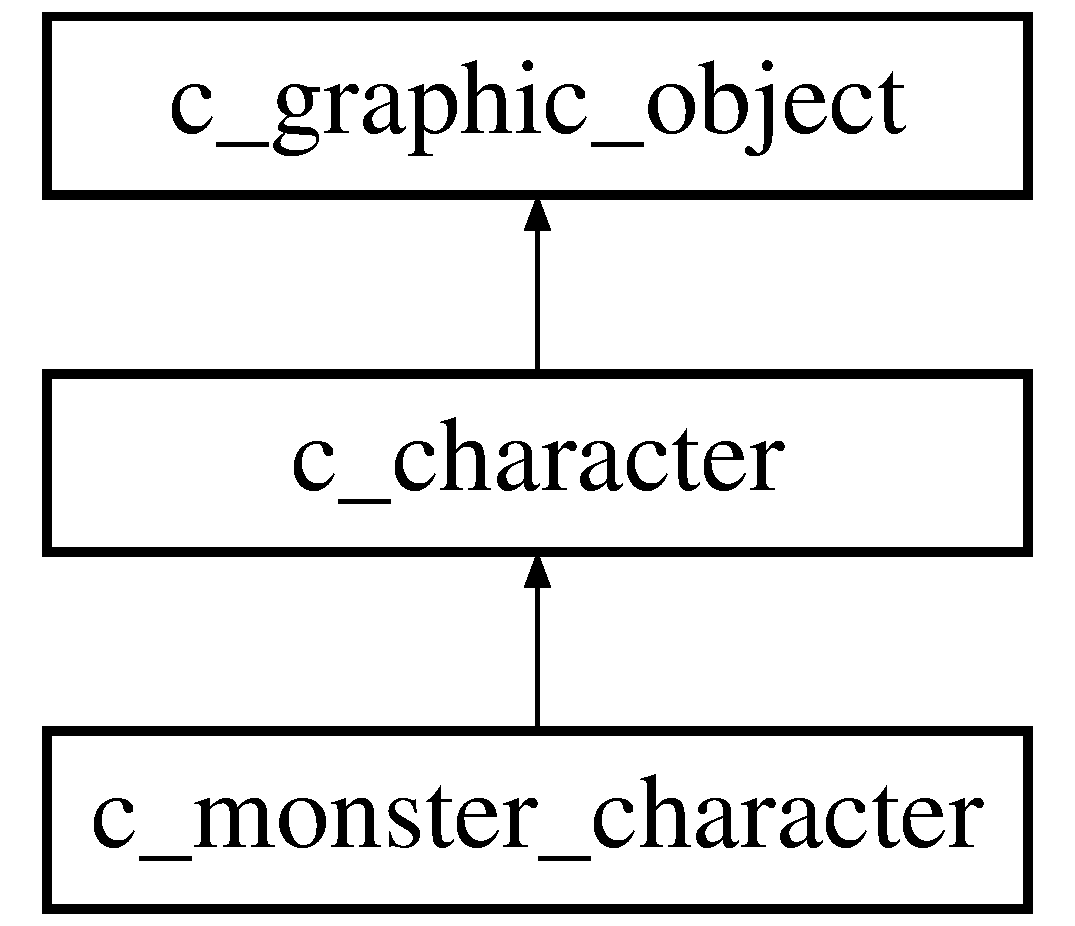
\includegraphics[height=3.000000cm]{classc__monster__character}
\end{center}
\end{figure}
\subsection*{Public Member Functions}
\begin{DoxyCompactItemize}
\item 
\hyperlink{classc__monster__character_aa2c75305c0f964c08d92bbf9af37d055}{c\-\_\-monster\-\_\-character} (t\-\_\-monster\-\_\-type type, int square\-\_\-x, int square\-\_\-y, long $\ast$\hyperlink{classc__graphic__object_a9ff91aa7a60272a8f713ff011a0cc0bb}{global\-\_\-time})
\item 
\hyperlink{classc__monster__character_ae71c6e9894ba46d21f14730e018aa0a9}{$\sim$c\-\_\-monster\-\_\-character} ()
\item 
t\-\_\-monster\-\_\-type \hyperlink{classc__monster__character_a1e60ad834fcdb5cf8c5dc68b708116a4}{get\-\_\-monster\-\_\-type} ()
\item 
void \hyperlink{classc__monster__character_a41087457a2b7222423fb6b222cc650bf}{add\-\_\-path\-\_\-instruction} (t\-\_\-direction \hyperlink{classc__character_a571f1ae6115d7e9fee3159c41fcf27e8}{direction}, int number\-\_\-of\-\_\-steps)
\item 
t\-\_\-direction \hyperlink{classc__monster__character_a07f29e8aae5420c20a706c5449bd22ae}{get\-\_\-next\-\_\-move} ()
\item 
void \hyperlink{classc__monster__character_ad70a99a00e0c7cd66955815a0eb2634b}{start\-\_\-moving} ()
\item 
virtual void \hyperlink{classc__monster__character_ac400987c335adde2454cab352a63d3d2}{draw} (int x, int y)
\end{DoxyCompactItemize}
\subsection*{Protected Member Functions}
\begin{DoxyCompactItemize}
\item 
void \hyperlink{classc__monster__character_a7e18086daeeb6d96c0993ce2edf84f00}{next\-\_\-instruction} ()
\end{DoxyCompactItemize}
\subsection*{Protected Attributes}
\begin{DoxyCompactItemize}
\item 
\hypertarget{classc__monster__character_a40b514f9d091ee513c10e2d9b57bb3e5}{t\-\_\-monster\-\_\-type {\bfseries type}}\label{classc__monster__character_a40b514f9d091ee513c10e2d9b57bb3e5}

\item 
int \hyperlink{classc__monster__character_a2ccaf3ff00ff2370eac007960bd01d7b}{path\-\_\-length}
\item 
int \hyperlink{classc__monster__character_a26c7d28a5741c7b99caf7ec9acb80872}{current\-\_\-path\-\_\-instruction}
\item 
double \hyperlink{classc__monster__character_a4918cf31bdf7a308f57cc924fd48cd49}{goes\-\_\-to}
\item 
t\-\_\-direction \hyperlink{classc__monster__character_a6182d1b0f70221c2fdde578cdee0d6e2}{path\-\_\-directions} \mbox{[}M\-A\-X\-\_\-\-M\-O\-N\-S\-T\-E\-R\-\_\-\-P\-A\-T\-H\-\_\-\-L\-E\-N\-G\-T\-H\mbox{]}
\item 
int \hyperlink{classc__monster__character_ab4531ab1220b9a52fd07b290350bba05}{path\-\_\-steps} \mbox{[}M\-A\-X\-\_\-\-M\-O\-N\-S\-T\-E\-R\-\_\-\-P\-A\-T\-H\-\_\-\-L\-E\-N\-G\-T\-H\mbox{]}
\item 
bool \hyperlink{classc__monster__character_abea3e334122c075498889efb7a476b58}{is\-\_\-dead}
\item 
bool \hyperlink{classc__monster__character_ad751b3e9f92c8b0496bd936c66a7598c}{waiting}
\item 
double \hyperlink{classc__monster__character_a944e8c78c13e1ec2169b59287ea5ef1c}{waiting\-\_\-end}
\end{DoxyCompactItemize}
\subsection*{Additional Inherited Members}


\subsection{Detailed Description}
Monster character class header file.

authors\-: Miloslav Číž year\-: 2013 

\subsection{Constructor \& Destructor Documentation}
\hypertarget{classc__monster__character_aa2c75305c0f964c08d92bbf9af37d055}{\index{c\-\_\-monster\-\_\-character@{c\-\_\-monster\-\_\-character}!c\-\_\-monster\-\_\-character@{c\-\_\-monster\-\_\-character}}
\index{c\-\_\-monster\-\_\-character@{c\-\_\-monster\-\_\-character}!c_monster_character@{c\-\_\-monster\-\_\-character}}
\subsubsection[{c\-\_\-monster\-\_\-character}]{\setlength{\rightskip}{0pt plus 5cm}c\-\_\-monster\-\_\-character\-::c\-\_\-monster\-\_\-character (
\begin{DoxyParamCaption}
\item[{t\-\_\-monster\-\_\-type}]{type, }
\item[{int}]{square\-\_\-x, }
\item[{int}]{square\-\_\-y, }
\item[{long $\ast$}]{global\-\_\-time}
\end{DoxyParamCaption}
)}}\label{classc__monster__character_aa2c75305c0f964c08d92bbf9af37d055}
Switches to the next path instruction.

Monster character class implementation file.

authors\-: Miloslav Číž year\-: 2013 \hypertarget{classc__monster__character_ae71c6e9894ba46d21f14730e018aa0a9}{\index{c\-\_\-monster\-\_\-character@{c\-\_\-monster\-\_\-character}!$\sim$c\-\_\-monster\-\_\-character@{$\sim$c\-\_\-monster\-\_\-character}}
\index{$\sim$c\-\_\-monster\-\_\-character@{$\sim$c\-\_\-monster\-\_\-character}!c_monster_character@{c\-\_\-monster\-\_\-character}}
\subsubsection[{$\sim$c\-\_\-monster\-\_\-character}]{\setlength{\rightskip}{0pt plus 5cm}c\-\_\-monster\-\_\-character\-::$\sim$c\-\_\-monster\-\_\-character (
\begin{DoxyParamCaption}
{}
\end{DoxyParamCaption}
)}}\label{classc__monster__character_ae71c6e9894ba46d21f14730e018aa0a9}
Class constructor, creates a new object.


\begin{DoxyParams}{Parameters}
{\em type} & monster type to be set \\
\hline
{\em square\-\_\-x} & initial x position \\
\hline
{\em square\-\_\-y} & initial y position \\
\hline
{\em global\-\_\-time} & pointer to global time counter \\
\hline
\end{DoxyParams}


\subsection{Member Function Documentation}
\hypertarget{classc__monster__character_a41087457a2b7222423fb6b222cc650bf}{\index{c\-\_\-monster\-\_\-character@{c\-\_\-monster\-\_\-character}!add\-\_\-path\-\_\-instruction@{add\-\_\-path\-\_\-instruction}}
\index{add\-\_\-path\-\_\-instruction@{add\-\_\-path\-\_\-instruction}!c_monster_character@{c\-\_\-monster\-\_\-character}}
\subsubsection[{add\-\_\-path\-\_\-instruction}]{\setlength{\rightskip}{0pt plus 5cm}void c\-\_\-monster\-\_\-character\-::add\-\_\-path\-\_\-instruction (
\begin{DoxyParamCaption}
\item[{t\-\_\-direction}]{direction, }
\item[{int}]{number\-\_\-of\-\_\-steps}
\end{DoxyParamCaption}
)}}\label{classc__monster__character_a41087457a2b7222423fb6b222cc650bf}
Returns the monster's type. \hypertarget{classc__monster__character_ac400987c335adde2454cab352a63d3d2}{\index{c\-\_\-monster\-\_\-character@{c\-\_\-monster\-\_\-character}!draw@{draw}}
\index{draw@{draw}!c_monster_character@{c\-\_\-monster\-\_\-character}}
\subsubsection[{draw}]{\setlength{\rightskip}{0pt plus 5cm}void c\-\_\-monster\-\_\-character\-::draw (
\begin{DoxyParamCaption}
\item[{int}]{x, }
\item[{int}]{y}
\end{DoxyParamCaption}
)\hspace{0.3cm}{\ttfamily [virtual]}}}\label{classc__monster__character_ac400987c335adde2454cab352a63d3d2}
Starts the monster's movement, it's position and path should be set by the time this method is called. 

Reimplemented from \hyperlink{classc__graphic__object_a94ef8137eed9ce1ae7adf366fefb51cf}{c\-\_\-graphic\-\_\-object}.

\hypertarget{classc__monster__character_a1e60ad834fcdb5cf8c5dc68b708116a4}{\index{c\-\_\-monster\-\_\-character@{c\-\_\-monster\-\_\-character}!get\-\_\-monster\-\_\-type@{get\-\_\-monster\-\_\-type}}
\index{get\-\_\-monster\-\_\-type@{get\-\_\-monster\-\_\-type}!c_monster_character@{c\-\_\-monster\-\_\-character}}
\subsubsection[{get\-\_\-monster\-\_\-type}]{\setlength{\rightskip}{0pt plus 5cm}t\-\_\-monster\-\_\-type c\-\_\-monster\-\_\-character\-::get\-\_\-monster\-\_\-type (
\begin{DoxyParamCaption}
{}
\end{DoxyParamCaption}
)}}\label{classc__monster__character_a1e60ad834fcdb5cf8c5dc68b708116a4}
Class destructor, frees it's memory. \hypertarget{classc__monster__character_a07f29e8aae5420c20a706c5449bd22ae}{\index{c\-\_\-monster\-\_\-character@{c\-\_\-monster\-\_\-character}!get\-\_\-next\-\_\-move@{get\-\_\-next\-\_\-move}}
\index{get\-\_\-next\-\_\-move@{get\-\_\-next\-\_\-move}!c_monster_character@{c\-\_\-monster\-\_\-character}}
\subsubsection[{get\-\_\-next\-\_\-move}]{\setlength{\rightskip}{0pt plus 5cm}t\-\_\-direction c\-\_\-monster\-\_\-character\-::get\-\_\-next\-\_\-move (
\begin{DoxyParamCaption}
{}
\end{DoxyParamCaption}
)}}\label{classc__monster__character_a07f29e8aae5420c20a706c5449bd22ae}
Adds a path instruction for the monster. There is a maximum of M\-A\-X\-\_\-\-M\-O\-N\-S\-T\-E\-R\-\_\-\-P\-A\-T\-H\-\_\-\-L\-E\-N\-G\-T\-H that can be added. Those are instructions for monster to make it's movement.


\begin{DoxyParams}{Parameters}
{\em direction} & direction in which to move \\
\hline
{\em number\-\_\-of\-\_\-steps} & number of steps to make in provided direction \\
\hline
\end{DoxyParams}
\hypertarget{classc__monster__character_a7e18086daeeb6d96c0993ce2edf84f00}{\index{c\-\_\-monster\-\_\-character@{c\-\_\-monster\-\_\-character}!next\-\_\-instruction@{next\-\_\-instruction}}
\index{next\-\_\-instruction@{next\-\_\-instruction}!c_monster_character@{c\-\_\-monster\-\_\-character}}
\subsubsection[{next\-\_\-instruction}]{\setlength{\rightskip}{0pt plus 5cm}void c\-\_\-monster\-\_\-character\-::next\-\_\-instruction (
\begin{DoxyParamCaption}
{}
\end{DoxyParamCaption}
)\hspace{0.3cm}{\ttfamily [protected]}}}\label{classc__monster__character_a7e18086daeeb6d96c0993ce2edf84f00}
end time of waiting \hypertarget{classc__monster__character_ad70a99a00e0c7cd66955815a0eb2634b}{\index{c\-\_\-monster\-\_\-character@{c\-\_\-monster\-\_\-character}!start\-\_\-moving@{start\-\_\-moving}}
\index{start\-\_\-moving@{start\-\_\-moving}!c_monster_character@{c\-\_\-monster\-\_\-character}}
\subsubsection[{start\-\_\-moving}]{\setlength{\rightskip}{0pt plus 5cm}void c\-\_\-monster\-\_\-character\-::start\-\_\-moving (
\begin{DoxyParamCaption}
{}
\end{DoxyParamCaption}
)}}\label{classc__monster__character_ad70a99a00e0c7cd66955815a0eb2634b}
Returns the direction in which the monster should move next;

\begin{DoxyReturn}{Returns}
direction in which monster should move (can be D\-I\-R\-E\-C\-T\-I\-O\-N\-\_\-\-N\-O\-N\-E which means it should wait) 
\end{DoxyReturn}


\subsection{Member Data Documentation}
\hypertarget{classc__monster__character_a26c7d28a5741c7b99caf7ec9acb80872}{\index{c\-\_\-monster\-\_\-character@{c\-\_\-monster\-\_\-character}!current\-\_\-path\-\_\-instruction@{current\-\_\-path\-\_\-instruction}}
\index{current\-\_\-path\-\_\-instruction@{current\-\_\-path\-\_\-instruction}!c_monster_character@{c\-\_\-monster\-\_\-character}}
\subsubsection[{current\-\_\-path\-\_\-instruction}]{\setlength{\rightskip}{0pt plus 5cm}int c\-\_\-monster\-\_\-character\-::current\-\_\-path\-\_\-instruction\hspace{0.3cm}{\ttfamily [protected]}}}\label{classc__monster__character_a26c7d28a5741c7b99caf7ec9acb80872}
length of path directions and path steps arrays \hypertarget{classc__monster__character_a4918cf31bdf7a308f57cc924fd48cd49}{\index{c\-\_\-monster\-\_\-character@{c\-\_\-monster\-\_\-character}!goes\-\_\-to@{goes\-\_\-to}}
\index{goes\-\_\-to@{goes\-\_\-to}!c_monster_character@{c\-\_\-monster\-\_\-character}}
\subsubsection[{goes\-\_\-to}]{\setlength{\rightskip}{0pt plus 5cm}double c\-\_\-monster\-\_\-character\-::goes\-\_\-to\hspace{0.3cm}{\ttfamily [protected]}}}\label{classc__monster__character_a4918cf31bdf7a308f57cc924fd48cd49}
current position in path arrays \hypertarget{classc__monster__character_abea3e334122c075498889efb7a476b58}{\index{c\-\_\-monster\-\_\-character@{c\-\_\-monster\-\_\-character}!is\-\_\-dead@{is\-\_\-dead}}
\index{is\-\_\-dead@{is\-\_\-dead}!c_monster_character@{c\-\_\-monster\-\_\-character}}
\subsubsection[{is\-\_\-dead}]{\setlength{\rightskip}{0pt plus 5cm}bool c\-\_\-monster\-\_\-character\-::is\-\_\-dead\hspace{0.3cm}{\ttfamily [protected]}}}\label{classc__monster__character_abea3e334122c075498889efb7a476b58}
contains sequence of number of steps that will be made in given directions \hypertarget{classc__monster__character_a6182d1b0f70221c2fdde578cdee0d6e2}{\index{c\-\_\-monster\-\_\-character@{c\-\_\-monster\-\_\-character}!path\-\_\-directions@{path\-\_\-directions}}
\index{path\-\_\-directions@{path\-\_\-directions}!c_monster_character@{c\-\_\-monster\-\_\-character}}
\subsubsection[{path\-\_\-directions}]{\setlength{\rightskip}{0pt plus 5cm}t\-\_\-direction c\-\_\-monster\-\_\-character\-::path\-\_\-directions\mbox{[}M\-A\-X\-\_\-\-M\-O\-N\-S\-T\-E\-R\-\_\-\-P\-A\-T\-H\-\_\-\-L\-E\-N\-G\-T\-H\mbox{]}\hspace{0.3cm}{\ttfamily [protected]}}}\label{classc__monster__character_a6182d1b0f70221c2fdde578cdee0d6e2}
x or y coordination (depending on direction) to which the character is headed by the current path instruction \hypertarget{classc__monster__character_a2ccaf3ff00ff2370eac007960bd01d7b}{\index{c\-\_\-monster\-\_\-character@{c\-\_\-monster\-\_\-character}!path\-\_\-length@{path\-\_\-length}}
\index{path\-\_\-length@{path\-\_\-length}!c_monster_character@{c\-\_\-monster\-\_\-character}}
\subsubsection[{path\-\_\-length}]{\setlength{\rightskip}{0pt plus 5cm}int c\-\_\-monster\-\_\-character\-::path\-\_\-length\hspace{0.3cm}{\ttfamily [protected]}}}\label{classc__monster__character_a2ccaf3ff00ff2370eac007960bd01d7b}
monster type \hypertarget{classc__monster__character_ab4531ab1220b9a52fd07b290350bba05}{\index{c\-\_\-monster\-\_\-character@{c\-\_\-monster\-\_\-character}!path\-\_\-steps@{path\-\_\-steps}}
\index{path\-\_\-steps@{path\-\_\-steps}!c_monster_character@{c\-\_\-monster\-\_\-character}}
\subsubsection[{path\-\_\-steps}]{\setlength{\rightskip}{0pt plus 5cm}int c\-\_\-monster\-\_\-character\-::path\-\_\-steps\mbox{[}M\-A\-X\-\_\-\-M\-O\-N\-S\-T\-E\-R\-\_\-\-P\-A\-T\-H\-\_\-\-L\-E\-N\-G\-T\-H\mbox{]}\hspace{0.3cm}{\ttfamily [protected]}}}\label{classc__monster__character_ab4531ab1220b9a52fd07b290350bba05}
contains sequence of directions in which steps are made \hypertarget{classc__monster__character_ad751b3e9f92c8b0496bd936c66a7598c}{\index{c\-\_\-monster\-\_\-character@{c\-\_\-monster\-\_\-character}!waiting@{waiting}}
\index{waiting@{waiting}!c_monster_character@{c\-\_\-monster\-\_\-character}}
\subsubsection[{waiting}]{\setlength{\rightskip}{0pt plus 5cm}bool c\-\_\-monster\-\_\-character\-::waiting\hspace{0.3cm}{\ttfamily [protected]}}}\label{classc__monster__character_ad751b3e9f92c8b0496bd936c66a7598c}
whether the monster is dead \hypertarget{classc__monster__character_a944e8c78c13e1ec2169b59287ea5ef1c}{\index{c\-\_\-monster\-\_\-character@{c\-\_\-monster\-\_\-character}!waiting\-\_\-end@{waiting\-\_\-end}}
\index{waiting\-\_\-end@{waiting\-\_\-end}!c_monster_character@{c\-\_\-monster\-\_\-character}}
\subsubsection[{waiting\-\_\-end}]{\setlength{\rightskip}{0pt plus 5cm}double c\-\_\-monster\-\_\-character\-::waiting\-\_\-end\hspace{0.3cm}{\ttfamily [protected]}}}\label{classc__monster__character_a944e8c78c13e1ec2169b59287ea5ef1c}
whether the monster is waiting and not moving 

The documentation for this class was generated from the following files\-:\begin{DoxyCompactItemize}
\item 
magerage/monster\-\_\-character.\-h\item 
magerage/monster\-\_\-character.\-cpp\end{DoxyCompactItemize}

\hypertarget{classc__player__character}{\section{c\-\_\-player\-\_\-character Class Reference}
\label{classc__player__character}\index{c\-\_\-player\-\_\-character@{c\-\_\-player\-\_\-character}}
}


{\ttfamily \#include $<$player\-\_\-character.\-h$>$}

Inheritance diagram for c\-\_\-player\-\_\-character\-:\begin{figure}[H]
\begin{center}
\leavevmode
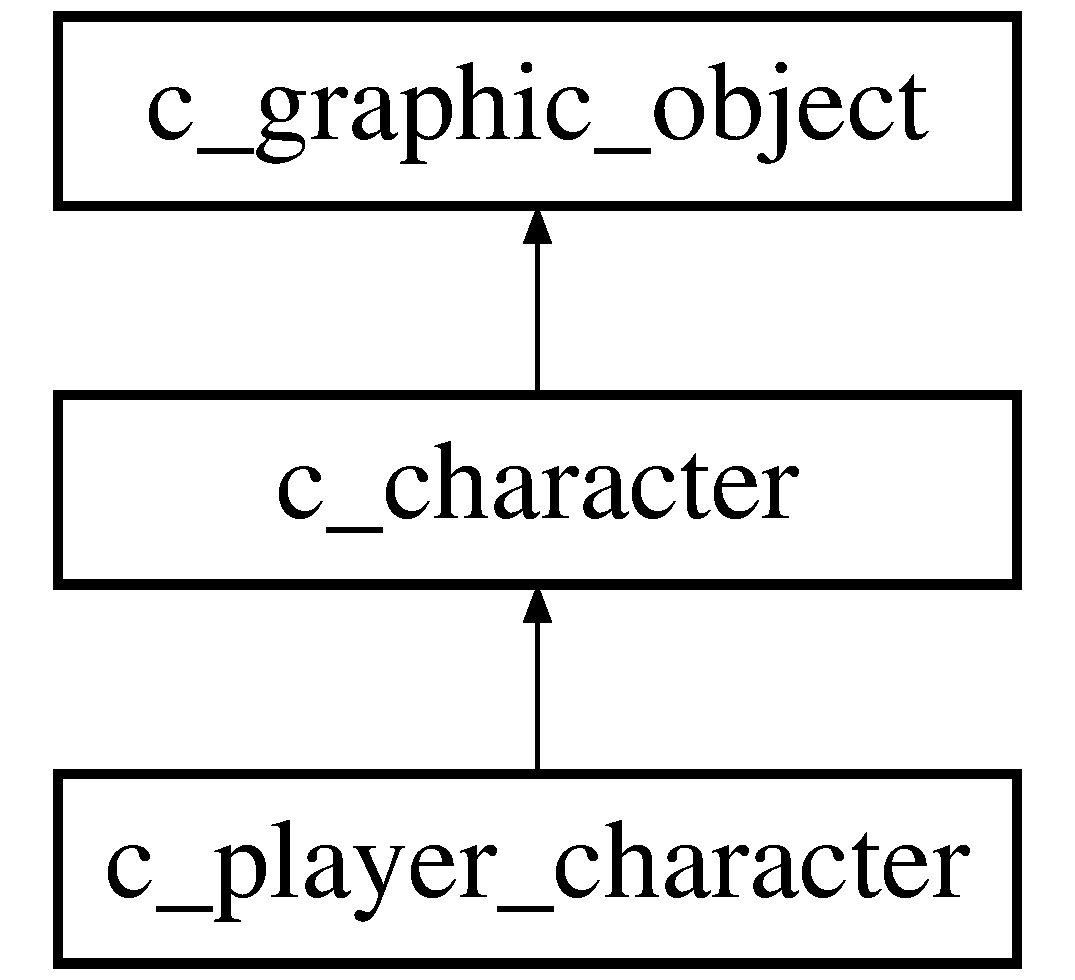
\includegraphics[height=3.000000cm]{classc__player__character}
\end{center}
\end{figure}
\subsection*{Public Member Functions}
\begin{DoxyCompactItemize}
\item 
\hyperlink{classc__player__character_a3779dab4cf22d1a5b9620ddae7fc11ef}{c\-\_\-player\-\_\-character} (t\-\_\-player\-\_\-type player\-\_\-type, long int $\ast$\hyperlink{classc__graphic__object_a9ff91aa7a60272a8f713ff011a0cc0bb}{global\-\_\-time})
\item 
\hyperlink{classc__player__character_a76c1d10523b82cc1683f435c10b4df60}{$\sim$c\-\_\-player\-\_\-character} ()
\item 
virtual void \hyperlink{classc__player__character_aa5d59edcb370d29b83ac0b2659ab0385}{update\-\_\-animation\-\_\-period} ()
\item 
virtual void \hyperlink{classc__player__character_a75d0ecbf8d1892422766f4f46ace576e}{draw} (int x, int y)
\item 
t\-\_\-player\-\_\-type \hyperlink{classc__player__character_ab284e034563a966f084a131de4472dbf}{get\-\_\-player\-\_\-type} ()
\item 
virtual void \hyperlink{classc__player__character_a6fd0d6503cd56998a4e2c8eb8695767b}{play\-\_\-animation} (t\-\_\-animation\-\_\-type animation)
\item 
void \hyperlink{classc__player__character_a84bc0fbb1f70bd2fa62edf89030cd070}{change\-\_\-magic\-\_\-energy} (int amount)
\item 
int \hyperlink{classc__player__character_a755e1fdb47029e1fc282a7cc2a5e0e88}{get\-\_\-magic\-\_\-energy} ()
\item 
void \hyperlink{classc__player__character_afe8f9b4f4a05e9c9c10df32988610cca}{set\-\_\-fire\-\_\-cloak} (bool state)
\item 
bool \hyperlink{classc__player__character_a10eeb77b1630c15fe16c36b244805430}{fire\-\_\-cloak\-\_\-is\-\_\-on} ()
\end{DoxyCompactItemize}
\subsection*{Additional Inherited Members}


\subsection{Detailed Description}
Player character class header file.

authors\-: Miloslav Číž year\-: 2013 

\subsection{Constructor \& Destructor Documentation}
\hypertarget{classc__player__character_a3779dab4cf22d1a5b9620ddae7fc11ef}{\index{c\-\_\-player\-\_\-character@{c\-\_\-player\-\_\-character}!c\-\_\-player\-\_\-character@{c\-\_\-player\-\_\-character}}
\index{c\-\_\-player\-\_\-character@{c\-\_\-player\-\_\-character}!c_player_character@{c\-\_\-player\-\_\-character}}
\subsubsection[{c\-\_\-player\-\_\-character}]{\setlength{\rightskip}{0pt plus 5cm}c\-\_\-player\-\_\-character\-::c\-\_\-player\-\_\-character (
\begin{DoxyParamCaption}
\item[{t\-\_\-player\-\_\-type}]{player\-\_\-type, }
\item[{long int $\ast$}]{global\-\_\-time}
\end{DoxyParamCaption}
)}}\label{classc__player__character_a3779dab4cf22d1a5b9620ddae7fc11ef}
id to stop looping sound

Player character class implementation file.

authors\-: Miloslav Číž year\-: 2013 \hypertarget{classc__player__character_a76c1d10523b82cc1683f435c10b4df60}{\index{c\-\_\-player\-\_\-character@{c\-\_\-player\-\_\-character}!$\sim$c\-\_\-player\-\_\-character@{$\sim$c\-\_\-player\-\_\-character}}
\index{$\sim$c\-\_\-player\-\_\-character@{$\sim$c\-\_\-player\-\_\-character}!c_player_character@{c\-\_\-player\-\_\-character}}
\subsubsection[{$\sim$c\-\_\-player\-\_\-character}]{\setlength{\rightskip}{0pt plus 5cm}c\-\_\-player\-\_\-character\-::$\sim$c\-\_\-player\-\_\-character (
\begin{DoxyParamCaption}
{}
\end{DoxyParamCaption}
)}}\label{classc__player__character_a76c1d10523b82cc1683f435c10b4df60}
Class constructor, initialises new player character.


\begin{DoxyParams}{Parameters}
{\em player\-\_\-type} & type of player character \\
\hline
{\em global\-\_\-time} & reference to a global time counter which is needed for animations \\
\hline
\end{DoxyParams}


\subsection{Member Function Documentation}
\hypertarget{classc__player__character_a84bc0fbb1f70bd2fa62edf89030cd070}{\index{c\-\_\-player\-\_\-character@{c\-\_\-player\-\_\-character}!change\-\_\-magic\-\_\-energy@{change\-\_\-magic\-\_\-energy}}
\index{change\-\_\-magic\-\_\-energy@{change\-\_\-magic\-\_\-energy}!c_player_character@{c\-\_\-player\-\_\-character}}
\subsubsection[{change\-\_\-magic\-\_\-energy}]{\setlength{\rightskip}{0pt plus 5cm}void c\-\_\-player\-\_\-character\-::change\-\_\-magic\-\_\-energy (
\begin{DoxyParamCaption}
\item[{int}]{amount}
\end{DoxyParamCaption}
)}}\label{classc__player__character_a84bc0fbb1f70bd2fa62edf89030cd070}
Plays given animation.


\begin{DoxyParams}{Parameters}
{\em animation} & animation to be played \\
\hline
\end{DoxyParams}
\hypertarget{classc__player__character_a75d0ecbf8d1892422766f4f46ace576e}{\index{c\-\_\-player\-\_\-character@{c\-\_\-player\-\_\-character}!draw@{draw}}
\index{draw@{draw}!c_player_character@{c\-\_\-player\-\_\-character}}
\subsubsection[{draw}]{\setlength{\rightskip}{0pt plus 5cm}void c\-\_\-player\-\_\-character\-::draw (
\begin{DoxyParamCaption}
\item[{int}]{x, }
\item[{int}]{y}
\end{DoxyParamCaption}
)\hspace{0.3cm}{\ttfamily [virtual]}}}\label{classc__player__character_a75d0ecbf8d1892422766f4f46ace576e}
Depending on current animation sets the animation period attribute. 

Reimplemented from \hyperlink{classc__graphic__object_a94ef8137eed9ce1ae7adf366fefb51cf}{c\-\_\-graphic\-\_\-object}.

\hypertarget{classc__player__character_a10eeb77b1630c15fe16c36b244805430}{\index{c\-\_\-player\-\_\-character@{c\-\_\-player\-\_\-character}!fire\-\_\-cloak\-\_\-is\-\_\-on@{fire\-\_\-cloak\-\_\-is\-\_\-on}}
\index{fire\-\_\-cloak\-\_\-is\-\_\-on@{fire\-\_\-cloak\-\_\-is\-\_\-on}!c_player_character@{c\-\_\-player\-\_\-character}}
\subsubsection[{fire\-\_\-cloak\-\_\-is\-\_\-on}]{\setlength{\rightskip}{0pt plus 5cm}bool c\-\_\-player\-\_\-character\-::fire\-\_\-cloak\-\_\-is\-\_\-on (
\begin{DoxyParamCaption}
{}
\end{DoxyParamCaption}
)}}\label{classc__player__character_a10eeb77b1630c15fe16c36b244805430}
Sets the fire cloak on or off for this player. Only works for Metodej.


\begin{DoxyParams}{Parameters}
{\em state} & if true, the fire cload will be set on, otherwise it will be set off \\
\hline
\end{DoxyParams}
\hypertarget{classc__player__character_a755e1fdb47029e1fc282a7cc2a5e0e88}{\index{c\-\_\-player\-\_\-character@{c\-\_\-player\-\_\-character}!get\-\_\-magic\-\_\-energy@{get\-\_\-magic\-\_\-energy}}
\index{get\-\_\-magic\-\_\-energy@{get\-\_\-magic\-\_\-energy}!c_player_character@{c\-\_\-player\-\_\-character}}
\subsubsection[{get\-\_\-magic\-\_\-energy}]{\setlength{\rightskip}{0pt plus 5cm}int c\-\_\-player\-\_\-character\-::get\-\_\-magic\-\_\-energy (
\begin{DoxyParamCaption}
{}
\end{DoxyParamCaption}
)}}\label{classc__player__character_a755e1fdb47029e1fc282a7cc2a5e0e88}
Takes or gives an amount of magic energy from or to the player.


\begin{DoxyParams}{Parameters}
{\em amount} & amount of energy to be added, this can be also a negative number -\/ if the player already has full amount of energy or zero energy, no overflow will occur \\
\hline
\end{DoxyParams}
\hypertarget{classc__player__character_ab284e034563a966f084a131de4472dbf}{\index{c\-\_\-player\-\_\-character@{c\-\_\-player\-\_\-character}!get\-\_\-player\-\_\-type@{get\-\_\-player\-\_\-type}}
\index{get\-\_\-player\-\_\-type@{get\-\_\-player\-\_\-type}!c_player_character@{c\-\_\-player\-\_\-character}}
\subsubsection[{get\-\_\-player\-\_\-type}]{\setlength{\rightskip}{0pt plus 5cm}t\-\_\-player\-\_\-type c\-\_\-player\-\_\-character\-::get\-\_\-player\-\_\-type (
\begin{DoxyParamCaption}
{}
\end{DoxyParamCaption}
)}}\label{classc__player__character_ab284e034563a966f084a131de4472dbf}
Draws player character at given position.


\begin{DoxyParams}{Parameters}
{\em x} & x position on the scrren \\
\hline
{\em y} & y position on the screen \\
\hline
\end{DoxyParams}
\hypertarget{classc__player__character_a6fd0d6503cd56998a4e2c8eb8695767b}{\index{c\-\_\-player\-\_\-character@{c\-\_\-player\-\_\-character}!play\-\_\-animation@{play\-\_\-animation}}
\index{play\-\_\-animation@{play\-\_\-animation}!c_player_character@{c\-\_\-player\-\_\-character}}
\subsubsection[{play\-\_\-animation}]{\setlength{\rightskip}{0pt plus 5cm}void c\-\_\-player\-\_\-character\-::play\-\_\-animation (
\begin{DoxyParamCaption}
\item[{t\-\_\-animation\-\_\-type}]{animation}
\end{DoxyParamCaption}
)\hspace{0.3cm}{\ttfamily [virtual]}}}\label{classc__player__character_a6fd0d6503cd56998a4e2c8eb8695767b}
Returns type of this character.

\begin{DoxyReturn}{Returns}
character type 
\end{DoxyReturn}


Reimplemented from \hyperlink{classc__graphic__object_aa87323c0df1b2e79cef78573b6096512}{c\-\_\-graphic\-\_\-object}.

\hypertarget{classc__player__character_afe8f9b4f4a05e9c9c10df32988610cca}{\index{c\-\_\-player\-\_\-character@{c\-\_\-player\-\_\-character}!set\-\_\-fire\-\_\-cloak@{set\-\_\-fire\-\_\-cloak}}
\index{set\-\_\-fire\-\_\-cloak@{set\-\_\-fire\-\_\-cloak}!c_player_character@{c\-\_\-player\-\_\-character}}
\subsubsection[{set\-\_\-fire\-\_\-cloak}]{\setlength{\rightskip}{0pt plus 5cm}void c\-\_\-player\-\_\-character\-::set\-\_\-fire\-\_\-cloak (
\begin{DoxyParamCaption}
\item[{bool}]{state}
\end{DoxyParamCaption}
)}}\label{classc__player__character_afe8f9b4f4a05e9c9c10df32988610cca}
Returns amount of the player's magic energy.

\begin{DoxyReturn}{Returns}
player's magic energy 
\end{DoxyReturn}
\hypertarget{classc__player__character_aa5d59edcb370d29b83ac0b2659ab0385}{\index{c\-\_\-player\-\_\-character@{c\-\_\-player\-\_\-character}!update\-\_\-animation\-\_\-period@{update\-\_\-animation\-\_\-period}}
\index{update\-\_\-animation\-\_\-period@{update\-\_\-animation\-\_\-period}!c_player_character@{c\-\_\-player\-\_\-character}}
\subsubsection[{update\-\_\-animation\-\_\-period}]{\setlength{\rightskip}{0pt plus 5cm}void c\-\_\-player\-\_\-character\-::update\-\_\-animation\-\_\-period (
\begin{DoxyParamCaption}
{}
\end{DoxyParamCaption}
)\hspace{0.3cm}{\ttfamily [virtual]}}}\label{classc__player__character_aa5d59edcb370d29b83ac0b2659ab0385}
Class destructor, frees it's memory. 

Reimplemented from \hyperlink{classc__graphic__object_a20fa3f61532b73f64f3307fd14b7dba6}{c\-\_\-graphic\-\_\-object}.



The documentation for this class was generated from the following files\-:\begin{DoxyCompactItemize}
\item 
magerage/player\-\_\-character.\-h\item 
magerage/player\-\_\-character.\-cpp\end{DoxyCompactItemize}

\hypertarget{structt__game__settings}{\section{t\-\_\-game\-\_\-settings Struct Reference}
\label{structt__game__settings}\index{t\-\_\-game\-\_\-settings@{t\-\_\-game\-\_\-settings}}
}


{\ttfamily \#include $<$game.\-h$>$}

\subsection*{Public Attributes}
\begin{DoxyCompactItemize}
\item 
bool \hyperlink{structt__game__settings_a33b533777d6fb82b3f8def6e26229597}{fullscreen}
\item 
bool \hyperlink{structt__game__settings_a3b1f22415c52a3b76d81cbd778b477bb}{music\-\_\-on}
\item 
int \hyperlink{structt__game__settings_a061c2e5b8aa3fcb84ffbce21025478e1}{sound\-\_\-volume}
\item 
int \hyperlink{structt__game__settings_aac810d731f668517630b182102e9fa7c}{last\-\_\-level}
\item 
string \hyperlink{structt__game__settings_a6b63568079b14532ae4acd05ba8488ff}{language}
\end{DoxyCompactItemize}


\subsection{Detailed Description}
Game class header file.

authors\-: Miloslav Číž year\-: 2013 

\subsection{Member Data Documentation}
\hypertarget{structt__game__settings_a33b533777d6fb82b3f8def6e26229597}{\index{t\-\_\-game\-\_\-settings@{t\-\_\-game\-\_\-settings}!fullscreen@{fullscreen}}
\index{fullscreen@{fullscreen}!t_game_settings@{t\-\_\-game\-\_\-settings}}
\subsubsection[{fullscreen}]{\setlength{\rightskip}{0pt plus 5cm}bool t\-\_\-game\-\_\-settings\-::fullscreen}}\label{structt__game__settings_a33b533777d6fb82b3f8def6e26229597}
Stores game settings. \hypertarget{structt__game__settings_a6b63568079b14532ae4acd05ba8488ff}{\index{t\-\_\-game\-\_\-settings@{t\-\_\-game\-\_\-settings}!language@{language}}
\index{language@{language}!t_game_settings@{t\-\_\-game\-\_\-settings}}
\subsubsection[{language}]{\setlength{\rightskip}{0pt plus 5cm}string t\-\_\-game\-\_\-settings\-::language}}\label{structt__game__settings_a6b63568079b14532ae4acd05ba8488ff}
the last level the player reached \hypertarget{structt__game__settings_aac810d731f668517630b182102e9fa7c}{\index{t\-\_\-game\-\_\-settings@{t\-\_\-game\-\_\-settings}!last\-\_\-level@{last\-\_\-level}}
\index{last\-\_\-level@{last\-\_\-level}!t_game_settings@{t\-\_\-game\-\_\-settings}}
\subsubsection[{last\-\_\-level}]{\setlength{\rightskip}{0pt plus 5cm}int t\-\_\-game\-\_\-settings\-::last\-\_\-level}}\label{structt__game__settings_aac810d731f668517630b182102e9fa7c}
sound volume in range 0 -\/ 100 \hypertarget{structt__game__settings_a3b1f22415c52a3b76d81cbd778b477bb}{\index{t\-\_\-game\-\_\-settings@{t\-\_\-game\-\_\-settings}!music\-\_\-on@{music\-\_\-on}}
\index{music\-\_\-on@{music\-\_\-on}!t_game_settings@{t\-\_\-game\-\_\-settings}}
\subsubsection[{music\-\_\-on}]{\setlength{\rightskip}{0pt plus 5cm}bool t\-\_\-game\-\_\-settings\-::music\-\_\-on}}\label{structt__game__settings_a3b1f22415c52a3b76d81cbd778b477bb}
whether the game is full screen or windowed \hypertarget{structt__game__settings_a061c2e5b8aa3fcb84ffbce21025478e1}{\index{t\-\_\-game\-\_\-settings@{t\-\_\-game\-\_\-settings}!sound\-\_\-volume@{sound\-\_\-volume}}
\index{sound\-\_\-volume@{sound\-\_\-volume}!t_game_settings@{t\-\_\-game\-\_\-settings}}
\subsubsection[{sound\-\_\-volume}]{\setlength{\rightskip}{0pt plus 5cm}int t\-\_\-game\-\_\-settings\-::sound\-\_\-volume}}\label{structt__game__settings_a061c2e5b8aa3fcb84ffbce21025478e1}
whether the music is on or off 

The documentation for this struct was generated from the following file\-:\begin{DoxyCompactItemize}
\item 
magerage/game.\-h\end{DoxyCompactItemize}

\hypertarget{structt__input__output__state}{\section{t\-\_\-input\-\_\-output\-\_\-state Struct Reference}
\label{structt__input__output__state}\index{t\-\_\-input\-\_\-output\-\_\-state@{t\-\_\-input\-\_\-output\-\_\-state}}
}
\subsection*{Public Attributes}
\begin{DoxyCompactItemize}
\item 
bool \hyperlink{structt__input__output__state_a3a7919d7cac4a16be272b9180e958c54}{key\-\_\-up}
\item 
bool \hyperlink{structt__input__output__state_af987d3e450c10a4e46b551f7aa1727d0}{key\-\_\-right}
\item 
bool \hyperlink{structt__input__output__state_aff3f4f05784c0a89291a2ac094f0a460}{key\-\_\-down}
\item 
bool \hyperlink{structt__input__output__state_a172f53bf31467a7570dee3edc04923ca}{key\-\_\-left}
\item 
bool \hyperlink{structt__input__output__state_a050ec7d2c78152a00db4e9ad1f3329ed}{key\-\_\-1}
\item 
bool \hyperlink{structt__input__output__state_a919f0b46728019de55dd02716f529364}{key\-\_\-2}
\item 
bool \hyperlink{structt__input__output__state_a24ef3f98deef214934007a0d88aeea82}{key\-\_\-3}
\item 
bool \hyperlink{structt__input__output__state_a30f2ccfec5fdb7c45df57d02a9967845}{key\-\_\-use}
\item 
bool \hyperlink{structt__input__output__state_a58c75f9aee14025fc22d16100a7b638b}{key\-\_\-cast\-\_\-1}
\item 
bool \hyperlink{structt__input__output__state_a84a4ec4b57148499b1ab2f25842fdac5}{key\-\_\-cast\-\_\-2}
\item 
bool \hyperlink{structt__input__output__state_a82487c01eb24e2339682b0b0c7f0edab}{key\-\_\-cast\-\_\-3}
\item 
bool \hyperlink{structt__input__output__state_a05ce15a5c21b6d6381220699a897ff0d}{key\-\_\-map\-\_\-explore}
\item 
bool \hyperlink{structt__input__output__state_a12366e6b5751103da0959aee7b55122b}{key\-\_\-back}
\item 
bool \hyperlink{structt__input__output__state_a5d93aef9032f6da00cc274bf4062f302}{mouse\-\_\-1}
\item 
int \hyperlink{structt__input__output__state_ade192d11582991da2533029506ad959e}{mouse\-\_\-x}
\item 
int \hyperlink{structt__input__output__state_aa9680f3841a1f09512cbfbfd961b8886}{mouse\-\_\-y}
\item 
int \hyperlink{structt__input__output__state_af03e61a9a04ba5fe1a572ec3ce654e47}{screen\-\_\-x}
\item 
int \hyperlink{structt__input__output__state_ab04e56c5d58491073a68614686e2fc53}{screen\-\_\-y}
\end{DoxyCompactItemize}


\subsection{Member Data Documentation}
\hypertarget{structt__input__output__state_a050ec7d2c78152a00db4e9ad1f3329ed}{\index{t\-\_\-input\-\_\-output\-\_\-state@{t\-\_\-input\-\_\-output\-\_\-state}!key\-\_\-1@{key\-\_\-1}}
\index{key\-\_\-1@{key\-\_\-1}!t_input_output_state@{t\-\_\-input\-\_\-output\-\_\-state}}
\subsubsection[{key\-\_\-1}]{\setlength{\rightskip}{0pt plus 5cm}bool t\-\_\-input\-\_\-output\-\_\-state\-::key\-\_\-1}}\label{structt__input__output__state_a050ec7d2c78152a00db4e9ad1f3329ed}
key left \hypertarget{structt__input__output__state_a919f0b46728019de55dd02716f529364}{\index{t\-\_\-input\-\_\-output\-\_\-state@{t\-\_\-input\-\_\-output\-\_\-state}!key\-\_\-2@{key\-\_\-2}}
\index{key\-\_\-2@{key\-\_\-2}!t_input_output_state@{t\-\_\-input\-\_\-output\-\_\-state}}
\subsubsection[{key\-\_\-2}]{\setlength{\rightskip}{0pt plus 5cm}bool t\-\_\-input\-\_\-output\-\_\-state\-::key\-\_\-2}}\label{structt__input__output__state_a919f0b46728019de55dd02716f529364}
key switch to player 1 \hypertarget{structt__input__output__state_a24ef3f98deef214934007a0d88aeea82}{\index{t\-\_\-input\-\_\-output\-\_\-state@{t\-\_\-input\-\_\-output\-\_\-state}!key\-\_\-3@{key\-\_\-3}}
\index{key\-\_\-3@{key\-\_\-3}!t_input_output_state@{t\-\_\-input\-\_\-output\-\_\-state}}
\subsubsection[{key\-\_\-3}]{\setlength{\rightskip}{0pt plus 5cm}bool t\-\_\-input\-\_\-output\-\_\-state\-::key\-\_\-3}}\label{structt__input__output__state_a24ef3f98deef214934007a0d88aeea82}
key switch to player 2 \hypertarget{structt__input__output__state_a12366e6b5751103da0959aee7b55122b}{\index{t\-\_\-input\-\_\-output\-\_\-state@{t\-\_\-input\-\_\-output\-\_\-state}!key\-\_\-back@{key\-\_\-back}}
\index{key\-\_\-back@{key\-\_\-back}!t_input_output_state@{t\-\_\-input\-\_\-output\-\_\-state}}
\subsubsection[{key\-\_\-back}]{\setlength{\rightskip}{0pt plus 5cm}bool t\-\_\-input\-\_\-output\-\_\-state\-::key\-\_\-back}}\label{structt__input__output__state_a12366e6b5751103da0959aee7b55122b}
key used to move camera freely to explore the map \hypertarget{structt__input__output__state_a58c75f9aee14025fc22d16100a7b638b}{\index{t\-\_\-input\-\_\-output\-\_\-state@{t\-\_\-input\-\_\-output\-\_\-state}!key\-\_\-cast\-\_\-1@{key\-\_\-cast\-\_\-1}}
\index{key\-\_\-cast\-\_\-1@{key\-\_\-cast\-\_\-1}!t_input_output_state@{t\-\_\-input\-\_\-output\-\_\-state}}
\subsubsection[{key\-\_\-cast\-\_\-1}]{\setlength{\rightskip}{0pt plus 5cm}bool t\-\_\-input\-\_\-output\-\_\-state\-::key\-\_\-cast\-\_\-1}}\label{structt__input__output__state_a58c75f9aee14025fc22d16100a7b638b}
key used to manipulate map objects \hypertarget{structt__input__output__state_a84a4ec4b57148499b1ab2f25842fdac5}{\index{t\-\_\-input\-\_\-output\-\_\-state@{t\-\_\-input\-\_\-output\-\_\-state}!key\-\_\-cast\-\_\-2@{key\-\_\-cast\-\_\-2}}
\index{key\-\_\-cast\-\_\-2@{key\-\_\-cast\-\_\-2}!t_input_output_state@{t\-\_\-input\-\_\-output\-\_\-state}}
\subsubsection[{key\-\_\-cast\-\_\-2}]{\setlength{\rightskip}{0pt plus 5cm}bool t\-\_\-input\-\_\-output\-\_\-state\-::key\-\_\-cast\-\_\-2}}\label{structt__input__output__state_a84a4ec4b57148499b1ab2f25842fdac5}
key used to cast spell 1 \hypertarget{structt__input__output__state_a82487c01eb24e2339682b0b0c7f0edab}{\index{t\-\_\-input\-\_\-output\-\_\-state@{t\-\_\-input\-\_\-output\-\_\-state}!key\-\_\-cast\-\_\-3@{key\-\_\-cast\-\_\-3}}
\index{key\-\_\-cast\-\_\-3@{key\-\_\-cast\-\_\-3}!t_input_output_state@{t\-\_\-input\-\_\-output\-\_\-state}}
\subsubsection[{key\-\_\-cast\-\_\-3}]{\setlength{\rightskip}{0pt plus 5cm}bool t\-\_\-input\-\_\-output\-\_\-state\-::key\-\_\-cast\-\_\-3}}\label{structt__input__output__state_a82487c01eb24e2339682b0b0c7f0edab}
key used to cast spell 2 \hypertarget{structt__input__output__state_aff3f4f05784c0a89291a2ac094f0a460}{\index{t\-\_\-input\-\_\-output\-\_\-state@{t\-\_\-input\-\_\-output\-\_\-state}!key\-\_\-down@{key\-\_\-down}}
\index{key\-\_\-down@{key\-\_\-down}!t_input_output_state@{t\-\_\-input\-\_\-output\-\_\-state}}
\subsubsection[{key\-\_\-down}]{\setlength{\rightskip}{0pt plus 5cm}bool t\-\_\-input\-\_\-output\-\_\-state\-::key\-\_\-down}}\label{structt__input__output__state_aff3f4f05784c0a89291a2ac094f0a460}
key right \hypertarget{structt__input__output__state_a172f53bf31467a7570dee3edc04923ca}{\index{t\-\_\-input\-\_\-output\-\_\-state@{t\-\_\-input\-\_\-output\-\_\-state}!key\-\_\-left@{key\-\_\-left}}
\index{key\-\_\-left@{key\-\_\-left}!t_input_output_state@{t\-\_\-input\-\_\-output\-\_\-state}}
\subsubsection[{key\-\_\-left}]{\setlength{\rightskip}{0pt plus 5cm}bool t\-\_\-input\-\_\-output\-\_\-state\-::key\-\_\-left}}\label{structt__input__output__state_a172f53bf31467a7570dee3edc04923ca}
key down \hypertarget{structt__input__output__state_a05ce15a5c21b6d6381220699a897ff0d}{\index{t\-\_\-input\-\_\-output\-\_\-state@{t\-\_\-input\-\_\-output\-\_\-state}!key\-\_\-map\-\_\-explore@{key\-\_\-map\-\_\-explore}}
\index{key\-\_\-map\-\_\-explore@{key\-\_\-map\-\_\-explore}!t_input_output_state@{t\-\_\-input\-\_\-output\-\_\-state}}
\subsubsection[{key\-\_\-map\-\_\-explore}]{\setlength{\rightskip}{0pt plus 5cm}bool t\-\_\-input\-\_\-output\-\_\-state\-::key\-\_\-map\-\_\-explore}}\label{structt__input__output__state_a05ce15a5c21b6d6381220699a897ff0d}
key used to cast spell 3 \hypertarget{structt__input__output__state_af987d3e450c10a4e46b551f7aa1727d0}{\index{t\-\_\-input\-\_\-output\-\_\-state@{t\-\_\-input\-\_\-output\-\_\-state}!key\-\_\-right@{key\-\_\-right}}
\index{key\-\_\-right@{key\-\_\-right}!t_input_output_state@{t\-\_\-input\-\_\-output\-\_\-state}}
\subsubsection[{key\-\_\-right}]{\setlength{\rightskip}{0pt plus 5cm}bool t\-\_\-input\-\_\-output\-\_\-state\-::key\-\_\-right}}\label{structt__input__output__state_af987d3e450c10a4e46b551f7aa1727d0}
key up \hypertarget{structt__input__output__state_a3a7919d7cac4a16be272b9180e958c54}{\index{t\-\_\-input\-\_\-output\-\_\-state@{t\-\_\-input\-\_\-output\-\_\-state}!key\-\_\-up@{key\-\_\-up}}
\index{key\-\_\-up@{key\-\_\-up}!t_input_output_state@{t\-\_\-input\-\_\-output\-\_\-state}}
\subsubsection[{key\-\_\-up}]{\setlength{\rightskip}{0pt plus 5cm}bool t\-\_\-input\-\_\-output\-\_\-state\-::key\-\_\-up}}\label{structt__input__output__state_a3a7919d7cac4a16be272b9180e958c54}
Holds information about input state, such as keys being pressed, mouse position and so on. Also stores information about the screen. \hypertarget{structt__input__output__state_a30f2ccfec5fdb7c45df57d02a9967845}{\index{t\-\_\-input\-\_\-output\-\_\-state@{t\-\_\-input\-\_\-output\-\_\-state}!key\-\_\-use@{key\-\_\-use}}
\index{key\-\_\-use@{key\-\_\-use}!t_input_output_state@{t\-\_\-input\-\_\-output\-\_\-state}}
\subsubsection[{key\-\_\-use}]{\setlength{\rightskip}{0pt plus 5cm}bool t\-\_\-input\-\_\-output\-\_\-state\-::key\-\_\-use}}\label{structt__input__output__state_a30f2ccfec5fdb7c45df57d02a9967845}
key switch to player 3 \hypertarget{structt__input__output__state_a5d93aef9032f6da00cc274bf4062f302}{\index{t\-\_\-input\-\_\-output\-\_\-state@{t\-\_\-input\-\_\-output\-\_\-state}!mouse\-\_\-1@{mouse\-\_\-1}}
\index{mouse\-\_\-1@{mouse\-\_\-1}!t_input_output_state@{t\-\_\-input\-\_\-output\-\_\-state}}
\subsubsection[{mouse\-\_\-1}]{\setlength{\rightskip}{0pt plus 5cm}bool t\-\_\-input\-\_\-output\-\_\-state\-::mouse\-\_\-1}}\label{structt__input__output__state_a5d93aef9032f6da00cc274bf4062f302}
key used to go back in menus and to pause the game \hypertarget{structt__input__output__state_ade192d11582991da2533029506ad959e}{\index{t\-\_\-input\-\_\-output\-\_\-state@{t\-\_\-input\-\_\-output\-\_\-state}!mouse\-\_\-x@{mouse\-\_\-x}}
\index{mouse\-\_\-x@{mouse\-\_\-x}!t_input_output_state@{t\-\_\-input\-\_\-output\-\_\-state}}
\subsubsection[{mouse\-\_\-x}]{\setlength{\rightskip}{0pt plus 5cm}int t\-\_\-input\-\_\-output\-\_\-state\-::mouse\-\_\-x}}\label{structt__input__output__state_ade192d11582991da2533029506ad959e}
mouse button 1 \hypertarget{structt__input__output__state_aa9680f3841a1f09512cbfbfd961b8886}{\index{t\-\_\-input\-\_\-output\-\_\-state@{t\-\_\-input\-\_\-output\-\_\-state}!mouse\-\_\-y@{mouse\-\_\-y}}
\index{mouse\-\_\-y@{mouse\-\_\-y}!t_input_output_state@{t\-\_\-input\-\_\-output\-\_\-state}}
\subsubsection[{mouse\-\_\-y}]{\setlength{\rightskip}{0pt plus 5cm}int t\-\_\-input\-\_\-output\-\_\-state\-::mouse\-\_\-y}}\label{structt__input__output__state_aa9680f3841a1f09512cbfbfd961b8886}
mouse x position \hypertarget{structt__input__output__state_af03e61a9a04ba5fe1a572ec3ce654e47}{\index{t\-\_\-input\-\_\-output\-\_\-state@{t\-\_\-input\-\_\-output\-\_\-state}!screen\-\_\-x@{screen\-\_\-x}}
\index{screen\-\_\-x@{screen\-\_\-x}!t_input_output_state@{t\-\_\-input\-\_\-output\-\_\-state}}
\subsubsection[{screen\-\_\-x}]{\setlength{\rightskip}{0pt plus 5cm}int t\-\_\-input\-\_\-output\-\_\-state\-::screen\-\_\-x}}\label{structt__input__output__state_af03e61a9a04ba5fe1a572ec3ce654e47}
mouse y position \hypertarget{structt__input__output__state_ab04e56c5d58491073a68614686e2fc53}{\index{t\-\_\-input\-\_\-output\-\_\-state@{t\-\_\-input\-\_\-output\-\_\-state}!screen\-\_\-y@{screen\-\_\-y}}
\index{screen\-\_\-y@{screen\-\_\-y}!t_input_output_state@{t\-\_\-input\-\_\-output\-\_\-state}}
\subsubsection[{screen\-\_\-y}]{\setlength{\rightskip}{0pt plus 5cm}int t\-\_\-input\-\_\-output\-\_\-state\-::screen\-\_\-y}}\label{structt__input__output__state_ab04e56c5d58491073a68614686e2fc53}
screen resolution x 

The documentation for this struct was generated from the following file\-:\begin{DoxyCompactItemize}
\item 
magerage/general.\-h\end{DoxyCompactItemize}

\hypertarget{structt__map__square}{\section{t\-\_\-map\-\_\-square Struct Reference}
\label{structt__map__square}\index{t\-\_\-map\-\_\-square@{t\-\_\-map\-\_\-square}}
}
\subsection*{Public Attributes}
\begin{DoxyCompactItemize}
\item 
int \hyperlink{structt__map__square_ad50f073f7cca47229656374c22daa9f8}{height}
\item 
t\-\_\-square\-\_\-type \hyperlink{structt__map__square_af17b226474485e797d61cce54a409666}{type}
\item 
\hyperlink{classc__map__object}{c\-\_\-map\-\_\-object} $\ast$ \hyperlink{structt__map__square_ac2715b549f3b3fb05bfb9b436d5cfc2d}{map\-\_\-objects} \mbox{[}M\-A\-X\-\_\-\-O\-B\-J\-E\-C\-T\-S\-\_\-\-P\-E\-R\-\_\-\-S\-Q\-U\-A\-R\-E\mbox{]}
\item 
\hyperlink{classc__animation}{c\-\_\-animation} $\ast$ \hyperlink{structt__map__square_a501ddc8f612fc58041bd1c7a11920a15}{animation}
\end{DoxyCompactItemize}


\subsection{Member Data Documentation}
\hypertarget{structt__map__square_a501ddc8f612fc58041bd1c7a11920a15}{\index{t\-\_\-map\-\_\-square@{t\-\_\-map\-\_\-square}!animation@{animation}}
\index{animation@{animation}!t_map_square@{t\-\_\-map\-\_\-square}}
\subsubsection[{animation}]{\setlength{\rightskip}{0pt plus 5cm}{\bf c\-\_\-animation}$\ast$ t\-\_\-map\-\_\-square\-::animation}}\label{structt__map__square_a501ddc8f612fc58041bd1c7a11920a15}
objects on this square (N\-U\-L\-L means no object) \hypertarget{structt__map__square_ad50f073f7cca47229656374c22daa9f8}{\index{t\-\_\-map\-\_\-square@{t\-\_\-map\-\_\-square}!height@{height}}
\index{height@{height}!t_map_square@{t\-\_\-map\-\_\-square}}
\subsubsection[{height}]{\setlength{\rightskip}{0pt plus 5cm}int t\-\_\-map\-\_\-square\-::height}}\label{structt__map__square_ad50f073f7cca47229656374c22daa9f8}
Holds info about one map square. \hypertarget{structt__map__square_ac2715b549f3b3fb05bfb9b436d5cfc2d}{\index{t\-\_\-map\-\_\-square@{t\-\_\-map\-\_\-square}!map\-\_\-objects@{map\-\_\-objects}}
\index{map\-\_\-objects@{map\-\_\-objects}!t_map_square@{t\-\_\-map\-\_\-square}}
\subsubsection[{map\-\_\-objects}]{\setlength{\rightskip}{0pt plus 5cm}{\bf c\-\_\-map\-\_\-object}$\ast$ t\-\_\-map\-\_\-square\-::map\-\_\-objects\mbox{[}M\-A\-X\-\_\-\-O\-B\-J\-E\-C\-T\-S\-\_\-\-P\-E\-R\-\_\-\-S\-Q\-U\-A\-R\-E\mbox{]}}}\label{structt__map__square_ac2715b549f3b3fb05bfb9b436d5cfc2d}
square type, like normal, water, ice and so on. \hypertarget{structt__map__square_af17b226474485e797d61cce54a409666}{\index{t\-\_\-map\-\_\-square@{t\-\_\-map\-\_\-square}!type@{type}}
\index{type@{type}!t_map_square@{t\-\_\-map\-\_\-square}}
\subsubsection[{type}]{\setlength{\rightskip}{0pt plus 5cm}t\-\_\-square\-\_\-type t\-\_\-map\-\_\-square\-::type}}\label{structt__map__square_af17b226474485e797d61cce54a409666}
square height, min is 0, max is 2 

The documentation for this struct was generated from the following file\-:\begin{DoxyCompactItemize}
\item 
magerage/map.\-h\end{DoxyCompactItemize}

\hypertarget{structt__missile}{\section{t\-\_\-missile Struct Reference}
\label{structt__missile}\index{t\-\_\-missile@{t\-\_\-missile}}
}
\subsection*{Public Attributes}
\begin{DoxyCompactItemize}
\item 
t\-\_\-missile\-\_\-type \hyperlink{structt__missile_afba313b8a83b91562bef1ccad8ff3f92}{type}
\item 
t\-\_\-direction \hyperlink{structt__missile_ae4dadc8f7d044549eee89b6a3269ea16}{direction}
\item 
double \hyperlink{structt__missile_ad3b6c8669fcc124c1937dbe83055c59c}{position\-\_\-x}
\item 
double \hyperlink{structt__missile_ab72534e808fc45603282f9728de6f9cc}{position\-\_\-y}
\item 
int \hyperlink{structt__missile_a4787f7554bd035014ca6b4d5b61f4149}{square\-\_\-y}
\item 
int \hyperlink{structt__missile_a0f63c73c2c0f46fc1187f4ab604b6859}{square\-\_\-x}
\item 
int \hyperlink{structt__missile_a6b80ab2e879a495fb9b9759a8764e995}{height}
\item 
A\-L\-L\-E\-G\-R\-O\-\_\-\-B\-I\-T\-M\-A\-P $\ast$ \hyperlink{structt__missile_ab9bf06a913015c3de3c23f1fe8870306}{bitmap}
\end{DoxyCompactItemize}


\subsection{Member Data Documentation}
\hypertarget{structt__missile_ab9bf06a913015c3de3c23f1fe8870306}{\index{t\-\_\-missile@{t\-\_\-missile}!bitmap@{bitmap}}
\index{bitmap@{bitmap}!t_missile@{t\-\_\-missile}}
\subsubsection[{bitmap}]{\setlength{\rightskip}{0pt plus 5cm}A\-L\-L\-E\-G\-R\-O\-\_\-\-B\-I\-T\-M\-A\-P$\ast$ t\-\_\-missile\-::bitmap}}\label{structt__missile_ab9bf06a913015c3de3c23f1fe8870306}
height level \hypertarget{structt__missile_ae4dadc8f7d044549eee89b6a3269ea16}{\index{t\-\_\-missile@{t\-\_\-missile}!direction@{direction}}
\index{direction@{direction}!t_missile@{t\-\_\-missile}}
\subsubsection[{direction}]{\setlength{\rightskip}{0pt plus 5cm}t\-\_\-direction t\-\_\-missile\-::direction}}\label{structt__missile_ae4dadc8f7d044549eee89b6a3269ea16}
missile type \hypertarget{structt__missile_a6b80ab2e879a495fb9b9759a8764e995}{\index{t\-\_\-missile@{t\-\_\-missile}!height@{height}}
\index{height@{height}!t_missile@{t\-\_\-missile}}
\subsubsection[{height}]{\setlength{\rightskip}{0pt plus 5cm}int t\-\_\-missile\-::height}}\label{structt__missile_a6b80ab2e879a495fb9b9759a8764e995}
x square position \hypertarget{structt__missile_ad3b6c8669fcc124c1937dbe83055c59c}{\index{t\-\_\-missile@{t\-\_\-missile}!position\-\_\-x@{position\-\_\-x}}
\index{position\-\_\-x@{position\-\_\-x}!t_missile@{t\-\_\-missile}}
\subsubsection[{position\-\_\-x}]{\setlength{\rightskip}{0pt plus 5cm}double t\-\_\-missile\-::position\-\_\-x}}\label{structt__missile_ad3b6c8669fcc124c1937dbe83055c59c}
direction in which the missile is going \hypertarget{structt__missile_ab72534e808fc45603282f9728de6f9cc}{\index{t\-\_\-missile@{t\-\_\-missile}!position\-\_\-y@{position\-\_\-y}}
\index{position\-\_\-y@{position\-\_\-y}!t_missile@{t\-\_\-missile}}
\subsubsection[{position\-\_\-y}]{\setlength{\rightskip}{0pt plus 5cm}double t\-\_\-missile\-::position\-\_\-y}}\label{structt__missile_ab72534e808fc45603282f9728de6f9cc}
current x position \hypertarget{structt__missile_a0f63c73c2c0f46fc1187f4ab604b6859}{\index{t\-\_\-missile@{t\-\_\-missile}!square\-\_\-x@{square\-\_\-x}}
\index{square\-\_\-x@{square\-\_\-x}!t_missile@{t\-\_\-missile}}
\subsubsection[{square\-\_\-x}]{\setlength{\rightskip}{0pt plus 5cm}int t\-\_\-missile\-::square\-\_\-x}}\label{structt__missile_a0f63c73c2c0f46fc1187f4ab604b6859}
y square position \hypertarget{structt__missile_a4787f7554bd035014ca6b4d5b61f4149}{\index{t\-\_\-missile@{t\-\_\-missile}!square\-\_\-y@{square\-\_\-y}}
\index{square\-\_\-y@{square\-\_\-y}!t_missile@{t\-\_\-missile}}
\subsubsection[{square\-\_\-y}]{\setlength{\rightskip}{0pt plus 5cm}int t\-\_\-missile\-::square\-\_\-y}}\label{structt__missile_a4787f7554bd035014ca6b4d5b61f4149}
current y position \hypertarget{structt__missile_afba313b8a83b91562bef1ccad8ff3f92}{\index{t\-\_\-missile@{t\-\_\-missile}!type@{type}}
\index{type@{type}!t_missile@{t\-\_\-missile}}
\subsubsection[{type}]{\setlength{\rightskip}{0pt plus 5cm}t\-\_\-missile\-\_\-type t\-\_\-missile\-::type}}\label{structt__missile_afba313b8a83b91562bef1ccad8ff3f92}
Represents a magical missile. 

The documentation for this struct was generated from the following file\-:\begin{DoxyCompactItemize}
\item 
magerage/map.\-h\end{DoxyCompactItemize}

%--- End generated contents ---

% Index
\newpage
\phantomsection
\addcontentsline{toc}{part}{Index}
\printindex

\end{document}
